%**************************************%
%*    Generated from PreTeXt source   *%
%*    on 2017-12-11T22:07:39-07:00    *%
%*                                    *%
%*   http://mathbook.pugetsound.edu   *%
%*                                    *%
%**************************************%
\documentclass[10pt,]{book}
%% Custom Preamble Entries, early (use latex.preamble.early)
%% Inline math delimiters, \(, \), need to be robust
%% 2016-01-31:  latexrelease.sty  supersedes  fixltx2e.sty
%% If  latexrelease.sty  exists, bugfix is in kernel
%% If not, bugfix is in  fixltx2e.sty
%% See:  https://tug.org/TUGboat/tb36-3/tb114ltnews22.pdf
%% and read "Fewer fragile commands" in distribution's  latexchanges.pdf
\IfFileExists{latexrelease.sty}{}{\usepackage{fixltx2e}}
%% Text height identically 9 inches, text width varies on point size
%% See Bringhurst 2.1.1 on measure for recommendations
%% 75 characters per line (count spaces, punctuation) is target
%% which is the upper limit of Bringhurst's recommendations
%% Load geometry package to allow page margin adjustments
\usepackage{geometry}
\geometry{letterpaper,total={340pt,9.0in}}
%% Custom Page Layout Adjustments (use latex.geometry)
\geometry{papersize={7in,10in},  width=5in, inner=.75in, height=8.25in, top=0.75in, twoside, ignoreheadfoot}
%% This LaTeX file may be compiled with pdflatex, xelatex, or lualatex
%% The following provides engine-specific capabilities
%% Generally, xelatex and lualatex will do better languages other than US English
%% You can pick from the conditional if you will only ever use one engine
\usepackage{ifthen}
\usepackage{ifxetex,ifluatex}
\ifthenelse{\boolean{xetex} \or \boolean{luatex}}{%
%% begin: xelatex and lualatex-specific configuration
%% fontspec package will make Latin Modern (lmodern) the default font
\ifxetex\usepackage{xltxtra}\fi
\usepackage{fontspec}
%% realscripts is the only part of xltxtra relevant to lualatex 
\ifluatex\usepackage{realscripts}\fi
%% 
%% Extensive support for other languages
\usepackage{polyglossia}
%% Main document language is US English
\setdefaultlanguage{english}
%% Spanish
\setotherlanguage{spanish}
%% Vietnamese
\setotherlanguage{vietnamese}
%% end: xelatex and lualatex-specific configuration
}{%
%% begin: pdflatex-specific configuration
%% translate common Unicode to their LaTeX equivalents
%% Also, fontenc with T1 makes CM-Super the default font
%% (\input{ix-utf8enc.dfu} from the "inputenx" package is possible addition (broken?)
\usepackage[T1]{fontenc}
\usepackage[utf8]{inputenc}
%% end: pdflatex-specific configuration
}
%% Monospace font: Inconsolata (zi4)
%% Sponsored by TUG: http://levien.com/type/myfonts/inconsolata.html
%% See package documentation for excellent instructions
%% One caveat, seem to need full file name to locate OTF files
%% Loads the "upquote" package as needed, so we don't have to
%% Upright quotes might come from the  textcomp  package, which we also use
%% We employ the shapely \ell to match Google Font version
%% pdflatex: "varqu" option produces best upright quotes
%% xelatex,lualatex: add StylisticSet 1 for shapely \ell
%% xelatex,lualatex: add StylisticSet 2 for plain zero
%% xelatex,lualatex: we add StylisticSet 3 for upright quotes
%% 
\ifthenelse{\boolean{xetex} \or \boolean{luatex}}{%
%% begin: xelatex and lualatex-specific monospace font
\usepackage{zi4}
\setmonofont[BoldFont=Inconsolatazi4-Bold.otf,StylisticSet={1,3}]{Inconsolatazi4-Regular.otf}
%% end: xelatex and lualatex-specific monospace font
}{%
%% begin: pdflatex-specific monospace font
%% "varqu" option provides textcomp \textquotedbl glyph
%% "varl"  option provides shapely "ell"
\usepackage[varqu,varl]{zi4}
%% end: pdflatex-specific monospace font
}
%% Symbols, align environment, bracket-matrix
\usepackage{amsmath}
\usepackage{amssymb}
%% allow page breaks within display mathematics anywhere
%% level 4 is maximally permissive
%% this is exactly the opposite of AMSmath package philosophy
%% there are per-display, and per-equation options to control this
%% split, aligned, gathered, and alignedat are not affected
\allowdisplaybreaks[4]
%% allow more columns to a matrix
%% can make this even bigger by overriding with  latex.preamble.late  processing option
\setcounter{MaxMatrixCols}{30}
%%
%% Color support, xcolor package
%% Always loaded.  Used for:
%% mdframed boxes, add/delete text, author tools
\PassOptionsToPackage{usenames,dvipsnames,svgnames,table}{xcolor}
\usepackage{xcolor}
%%
%% Semantic Macros
%% To preserve meaning in a LaTeX file
%% Only defined here if required in this document
%% Used for inline definitions of terms
\newcommand{\terminology}[1]{\textbf{#1}}
%% Used to markup initialisms, text or titles
%% default is small caps (Bringhurst, 4e, 3.2.2, p. 48)
%% Titles are no-ops now, see comments in XSL source
\newcommand{\initialism}[1]{\textsc{\MakeLowercase{#1}}}
\DeclareRobustCommand{\initialismintitle}[1]{\texorpdfstring{#1}{#1}}
%% Subdivision Numbering, Chapters, Sections, Subsections, etc
%% Subdivision numbers may be turned off at some level ("depth")
%% A section *always* has depth 1, contrary to us counting from the document root
%% The latex default is 3.  If a larger number is present here, then
%% removing this command may make some cross-references ambiguous
%% The precursor variable $numbering-maxlevel is checked for consistency in the common XSL file
\setcounter{secnumdepth}{2}
%% Environments with amsthm package
%% Theorem-like environments in "plain" style, with or without proof
\usepackage{amsthm}
\theoremstyle{plain}
%% Numbering for Theorems, Conjectures, Examples, Figures, etc
%% Controlled by  numbering.theorems.level  processing parameter
%% Always need a theorem environment to set base numbering scheme
%% even if document has no theorems (but has other environments)
\newtheorem{theorem}{Theorem}[section]
%% Only variants actually used in document appear here
%% Style is like a theorem, and for statements without proofs
%% Numbering: all theorem-like numbered consecutively
%% i.e. Corollary 4.3 follows Theorem 4.2
\newtheorem{corollary}[theorem]{Corollary}
%% Numbering for Projects (independent of others)
%% Controlled by  numbering.projects.level  processing parameter
%% Always need a project environment to set base numbering scheme
%% even if document has no projectss (but has other blocks)
\newtheorem{project}{Project}%% Project-like environments, normal text
\theoremstyle{definition}
\newtheorem{activity}[project]{Problem}
%% Numbering for inline exercises is in sync with theorems, normal text
\theoremstyle{definition}
\newtheorem{exercise}[theorem]{Problem}
%% Localize LaTeX supplied names (possibly none)
\renewcommand*{\appendixname}{Appendix}
\renewcommand*{\chaptername}{Chapter}
%% Equation Numbering
%% Controlled by  numbering.equations.level  processing parameter
\numberwithin{equation}{chapter}
%% For improved tables
\usepackage{array}
%% Some extra height on each row is desirable, especially with horizontal rules
%% Increment determined experimentally
\setlength{\extrarowheight}{0.2ex}
%% Define variable thickness horizontal rules, full and partial
%% Thicknesses are 0.03, 0.05, 0.08 in the  booktabs  package
\makeatletter
\newcommand{\hrulethin}  {\noalign{\hrule height 0.04em}}
\newcommand{\hrulemedium}{\noalign{\hrule height 0.07em}}
\newcommand{\hrulethick} {\noalign{\hrule height 0.11em}}
%% We preserve a copy of the \setlength package before other
%% packages (extpfeil) get a chance to load packages that redefine it
\let\oldsetlength\setlength
\newlength{\Oldarrayrulewidth}
\newcommand{\crulethin}[1]%
{\noalign{\global\oldsetlength{\Oldarrayrulewidth}{\arrayrulewidth}}%
\noalign{\global\oldsetlength{\arrayrulewidth}{0.04em}}\cline{#1}%
\noalign{\global\oldsetlength{\arrayrulewidth}{\Oldarrayrulewidth}}}%
\newcommand{\crulemedium}[1]%
{\noalign{\global\oldsetlength{\Oldarrayrulewidth}{\arrayrulewidth}}%
\noalign{\global\oldsetlength{\arrayrulewidth}{0.07em}}\cline{#1}%
\noalign{\global\oldsetlength{\arrayrulewidth}{\Oldarrayrulewidth}}}
\newcommand{\crulethick}[1]%
{\noalign{\global\oldsetlength{\Oldarrayrulewidth}{\arrayrulewidth}}%
\noalign{\global\oldsetlength{\arrayrulewidth}{0.11em}}\cline{#1}%
\noalign{\global\oldsetlength{\arrayrulewidth}{\Oldarrayrulewidth}}}
%% Single letter column specifiers defined via array package
\newcolumntype{A}{!{\vrule width 0.04em}}
\newcolumntype{B}{!{\vrule width 0.07em}}
\newcolumntype{C}{!{\vrule width 0.11em}}
\makeatother
\newcommand{\tablecelllines}[3]%
{\begin{tabular}[#2]{@{}#1@{}}#3\end{tabular}}
%% Figures, Tables, Listings, Named Lists, Floats
%% The [H]ere option of the float package fixes floats in-place,
%% in deference to web usage, where floats are totally irrelevant
%% You can remove some of this setup, to restore standard LaTeX behavior
%% HOWEVER, numbering of figures/tables AND theorems/examples/remarks, etc
%% may de-synchronize with the numbering in the HTML version
%% You can remove the "placement={H}" option to allow flotation and
%% preserve numbering, BUT the numbering may then appear "out-of-order"
%% Floating environments: http://tex.stackexchange.com/questions/95631/
\usepackage{float}
\usepackage{newfloat}
\usepackage{caption}%% Adjust stock figure environment so that it no longer floats
\SetupFloatingEnvironment{figure}{fileext=lof,placement={H},within=section,name=Figure}
\captionsetup[figure]{labelfont=bf}
%% http://tex.stackexchange.com/questions/16195
\makeatletter
\let\c@figure\c@theorem
\makeatother
%% Adjust stock table environment so that it no longer floats
\SetupFloatingEnvironment{table}{fileext=lot,placement={H},within=section,name=Table}
\captionsetup[table]{labelfont=bf}
%% http://tex.stackexchange.com/questions/16195
\makeatletter
\let\c@table\c@theorem
\makeatother
%% Footnote Numbering
%% We reset the footnote counter, as given by numbering.footnotes.level
\makeatletter\@addtoreset{footnote}{chapter}\makeatother
%% Raster graphics inclusion, wrapped figures in paragraphs
%% \resizebox sometimes used for images in side-by-side layout
\usepackage{graphicx}
%%
%% More flexible list management, esp. for references and exercises
%% But also for specifying labels (i.e. custom order) on nested lists
\usepackage{enumitem}
%% Lists of exercises in their own section, maximum depth 4
\newlist{exerciselist}{description}{4}
\setlist[exerciselist]{leftmargin=0pt,itemsep=1.0ex,topsep=1.0ex,partopsep=0pt,parsep=0pt}
%% Support for index creation
%% imakeidx package does not require extra pass (as with makeidx)
%% Title of the "Index" section set via a keyword
%% Language support for the "see" and "see also" phrases
\usepackage{imakeidx}
\makeindex[title=Index, intoc=true]
\renewcommand{\seename}{see}
\renewcommand{\alsoname}{see also}
%% hyperref driver does not need to be specified, it will be detected
\usepackage{hyperref}
%% configure hyperref's  \url  to match listings' inline verbatim
\renewcommand\UrlFont{\small\ttfamily}
%% Hyperlinking active in PDFs, all links solid and blue
\hypersetup{colorlinks=true,linkcolor=blue,citecolor=blue,filecolor=blue,urlcolor=blue}
\hypersetup{pdftitle={Combinatorics Through Guided Discovery}}
%% If you manually remove hyperref, leave in this next command
\providecommand\phantomsection{}
%% Graphics Preamble Entries
\usepackage{tikz}
\usepackage{tkz-graph}
\usepackage{tkz-euclide}
\usepackage{chemfig}
\usetikzlibrary{patterns}
\usetikzlibrary{positioning}
\usetikzlibrary{matrix,arrows}
\usetikzlibrary{calc}
\usetikzlibrary{shapes}
\usetikzlibrary{through,intersections,decorations,shadows,fadings}

\usepackage{pgfplots}

\tikzset{vertex/.style = {shape=circle, draw, minimum size = 3ex, inner sep = 2pt}}
\tikzset{svertex/.style = {shape=circle, draw, fill=gray, minimum size = 5pt, inner sep = 2pt}}
\tikzset{evertex/.style = {shape=ellipse, draw, minimum width = 6ex, inner sep = 2pt}}
\tikzset{dedge/.style = {->, > = latex'}}
%% If tikz has been loaded, replace ampersand with \amp macro
\ifdefined\tikzset
    \tikzset{ampersand replacement = \amp}
\fi
%% NB: calc redefines \setlength
\usepackage{calc}
%% used repeatedly for vertical dimensions of sidebyside panels
\newlength{\panelmax}
%% extpfeil package for certain extensible arrows,
%% as also provided by MathJax extension of the same name
%% NB: this package loads mtools, which loads calc, which redefines
%%     \setlength, so it can be removed if it seems to be in the 
%%     way and your math does not use:
%%     
%%     \xtwoheadrightarrow, \xtwoheadleftarrow, \xmapsto, \xlongequal, \xtofrom
%%     
%%     we have had to be extra careful with variable thickness
%%     lines in tables, and so also load this package late
\usepackage{extpfeil}
%% Custom Preamble Entries, late (use latex.preamble.late)
% Set up the emoji for the three fruit we use
\newfontfamily{\emojifont}{Symbola}
\usepackage{newunicodechar}
\newunicodechar{🍎}{\emojifont{🍎}} % Red apple 
\newunicodechar{🍐}{{\emojifont{🍐}}} % Pear 
\newunicodechar{🍌}{{\emojifont{🍌}}} % Banana 
% Redefine activity environment to get problem type labels
\usepackage{tabto, pdfcomment}\newcommand{\marginsymbol}[2][0]{\tabto*{#1}\makebox[1ex][r]{#2}\tabto*{\TabPrevPos}}%%%  This is a set of styles to include in the preamble of the generated latex code for the book Discrete Mathematics: an Open Introduction.


% \usepackage{bold-extra}
% \usepackage{marvosym} %for stop signs.
% \usepackage{textcomp}
% \usepackage{multicol}


% % FONT OPTIONS (pick one group to uncomment):

%newpx is my current favorite.  This should work on a TEXLive distribution, but on MiKTeX it initially gave me problems.  Running the update wizard to update MiKTeX then showed ``newpx'' as an available package (only since 8/11/15).  Perhaps just synchronizing in the package manager would do the same thing.  Even then, needed to run initexmf --mkmaps from the command line.
%You could always uncomment all of these to use the default computer modern font.
\usepackage[utf8]{inputenc}
\usepackage[T1]{fontenc}
\usepackage{newpxtext}
\usepackage[vvarbb,cmintegrals,cmbraces,bigdelims]{newpxmath}
\usepackage[scr=rsfso]{mathalfa}% \mathscr is fancier than \mathcal
\linespread{1.04}         % adds more leading (space between lines)
% quantifiers look strange, so change those back to normal:
	\DeclareSymbolFont{mysymbols}{OMS}{cmsy}{b}{n} %note we make the figures bold to better match newpx.  Replace the ``b'' with an ``m'' to undo this.
	%\SetSymbolFont{mysymbols}  {bold}{OMS}{cmsy}{b}{n}
	%\DeclareSymbolFont{myoperators}   {OT1}{cmr} {m}{n}
	%\SetSymbolFont{myoperators}{bold}{OT1}{cmr} {bx}{n}
	\DeclareMathSymbol{\forall}{\mathord}{mysymbols}{"38}
	\DeclareMathSymbol{\exists}{\mathord}{mysymbols}{"39}
	%\DeclareMathSymbol{\pm}{\mathbin}{mysymbols}{"06}
	%\DeclareMathSymbol{+}{\mathbin}{myoperators}{"2B}
	%\DeclareMathSymbol{-}{\mathbin}{mysymbols}{"00}
	%\DeclareMathSymbol{=}{\mathrel}{myoperators}{"3D}
	%%% Suggested by Kent Morrison to fix \nobreakspace issues:
	\DeclareTextCommand{\nobreakspace}{T1}{\leavevmode\nobreak\ }



%\usepackage[T1]{fontenc}
%\usepackage{newtxtext,newtxmath}


%\usepackage[bitstream-charter]{mathdesign}
%\usepackage[T1]{fontenc}

%\usepackage[proportional,space,scaled=1.064]{erewhon}
%\usepackage[erewhon,vvarbb,bigdelims]{newtxmath}
%\usepackage[T1]{fontenc}
%\renewcommand*\oldstylenums[1]{\textosf{#1}}





% % % % % % Other packages % % % % % % % %

% \usepackage{docmute}
% \usepackage{pdfpages}
%
% \usepackage{svg}
%
\usepackage[framemethod=tikz]{mdframed}



% % % % % % % % % % % % % %  END OF PACKAGES  % % % % % % % % % % % % % % % % % % %

%%%%%%%%%%%%%%%%%%%%%%%%%%%%%%%%%%%%%%%%%%%%%%%%%%%%%%%%%%%%%%%%%%%%%%%%
%%%%%%%%%%%%%%%%%  Nicely styled environments: %%%%%%%%%%%%%%%%%%%%%%%%%
%%%%%%%%%%%%%%%%%%%%%%%%%%%%%%%%%%%%%%%%%%%%%%%%%%%%%%%%%%%%%%%%%%%%%%%%

\usepackage{tcolorbox}
\tcbuselibrary{skins}
\tcbuselibrary{breakable}

\newcommand{\sslash}{\mathbin{/\mkern-6mu/}}

% \tcbuselibrary{theorems}
%
% \newtcbtheorem{myproblem}{Problem}{colback=green!5, colframe=black}{th}



%Create indented ``problem'' environment:
% \newmdtheoremenv[%
% leftmargin=1.5ex, %left/right margins for oneside
% rightmargin=1.5ex,
% roundcorner=0pt,
% topline=false,
% leftline=false,
% ]{mdproblem}[project]{Problem}
\tcbset{probstyle/.style={%
	breakable,
	enhanced,
	colback=white,
	colframe=black!60,
	toprule=0mm,
	leftrule=0mm,
	bottomrule=.5pt,
	rightrule=.5pt,
	% bottom=0pt,
	top=2pt,
	extras unbroken and last={drop lifted shadow},
	before skip=1em,
	after skip=.5em,
	sharp corners=all,
	% after upper*={\quad $\sslash$},
	% overlay last={%
	% 	% \node at ([yshift=1em,xshift=-1em]frame.south east) {$\sslash$};
	% 	\draw[#1, blue!20] ([xshift=-10pt, yshift=-5pt]frame.south east) -- ++(0,2.5em);
	% 	\draw[#1, blue!20] ([xshift=-5pt]frame.south east) -- ++(-3em,0);
	% 	},
	% overlay unbroken={%
	% 	% \node at ([yshift=1em,xshift=-1em]frame.south east) {$\sslash$};
	% 	\draw[#1, blue!20] ([xshift=-10pt, yshift=-5pt]frame.south east) -- ++(0,2.5em);
	% 	\draw[#1, blue!20] ([xshift=-5pt]frame.south east) -- ++(-3em,0);
	% 	}
	}
}


\newtheorem{myproblem}[project]{Problem}

%Redefine ``example'' to call the new mdexample, and put a paragraph break after it.
\renewenvironment{activity}{%
\begin{tcolorbox}[probstyle]
\begin{myproblem}
}{%
\end{myproblem}
\end{tcolorbox}
\par\medskip
}


%Fix widows and orphans (single lines at top/bottom of page):
\clubpenalty=10000
\widowpenalty=10000
\raggedbottom



%%%%%%%%%%%%%%%%%%%%%%%%%%%%%%%%%%%%%%%%%%
%%%%%%%  Headers and footers %%%%%%%%%%%%%
%%%%%%%%%%%%%%%%%%%%%%%%%%%%%%%%%%%%%%%%%%

\usepackage{fancyhdr}
\pagestyle{fancy}
\renewcommand{\chaptermark}[1]{\markboth{\thechapter.\ #1}{}} %Removes word "chapter" from the \leftmark.

\fancyhead{} % clear header fields
\fancyhead[LE]{{\footnotesize \textsl{\thepage}}~~ \textsc{\scriptsize \nouppercase{\leftmark}}}
\fancyhead[RO]{\textsc{\scriptsize \nouppercase{\rightmark}} ~~ {\footnotesize \textsl{\thepage}}  }
\fancyfoot{}





% %%%%%%%%%%%%%%%%%%%%%%%%%%%%%%%%%%%%%%%%%%
% %%%%%%%    Chapter headings  %%%%%%%%%%%%%
% %%%%%%%%%%%%%%%%%%%%%%%%%%%%%%%%%%%%%%%%%%
%
% \usepackage[bf,sc,center,outermarks]{titlesec}
%
%
% %%%%% FIX FOR BUG IN TITLESEC %%%%%%%%%%%
% \usepackage{etoolbox}
%
% \makeatletter
% \patchcmd{\ttlh@hang}{\parindent\z@}{\parindent\z@\leavevmode}{}{}
% \patchcmd{\ttlh@hang}{\noindent}{}{}{}
% \makeatother
% %%%%% END FIX %%%%%%%%%%%%%%%%%%%%%%%%%%%%
%
%
% \titleformat{\chapter}[display]
% 	{\Large\filcenter}
% 	{\rule[4pt]{.3\textwidth}{2pt} \hspace{2ex} \large\textsc{\chaptertitlename} \thechapter \hspace{3ex} \rule[4pt]{0.3\textwidth}{2pt} }
% 	{1pc}
% 	{\titlerule\vspace{1ex}\huge\textsc}
% 	[\vspace{.75ex}\titlerule]
% \titlespacing*{\chapter}{0pt}{-2em}{2em}
%
% \titleformat{\paragraph}[block]
%   {\normalfont\bfseries\filcenter}
%   {\theparagraph}
%   {}
%   {\textsc}
% %%%%%%%%%  End chapter/sectio headings %%%%%%%%%%%%%%%%%

%%% End of File.


%% Begin: Author-provided packages
%% (From  docinfo/latex-preamble/package  elements)
%% End: Author-provided packages
%% Begin: Author-provided macros
%% (From  docinfo/macros  element)
%% Plus three from MBX for XML characters
\newcommand{\cycle}[1]{\arraycolsep 5 pt
\left(\begin{array}#1\end{array}\right)}
\newcommand{\importantarrow}{\Rightarrow}
\newcommand{\qchoose}[2]{\left[{#1\atop#2}\right]_q}
\def\neg1choose#1#2{\left[{#1\atop#2}\right]_{-1}}
\newcommand{\bp}{
\begin{enumerate}{\setcounter{enumi}{\value{problemnumber}}}}
\newcommand{\ep}{\setcounter{problemnumber}{\value{enumi}}
\end{enumerate}}
\newcommand{\ignore}[1]{}
\renewcommand{\bottomfraction}{.8}
\renewcommand{\topfraction}{.8}
\newcommand{\apple}{\text{🍎}}
\newcommand{\ap}{\apple}
\newcommand{\banana}{\text{🍌}}
\newcommand{\ba}{\banana}
\newcommand{\pear}{\text{🍐}}
\newcommand{\pe}{\pear}
\DeclareMathOperator{\Fix}{Fix}
\DeclareMathOperator{\Orb}{Orb}
\newcommand{\F}{\mathcal{F}}
\newcommand{\lt}{<}
\newcommand{\gt}{>}
\newcommand{\amp}{&}
%% End: Author-provided macros
%% Title page information for book
\title{Combinatorics Through Guided Discovery}
\author{Kenneth P. Bogart\\
Dartmouth College
}
\date{}
\begin{document}
\frontmatter
%% begin: half-title
\thispagestyle{empty}
{\centering
\vspace*{0.28\textheight}
{\Huge Combinatorics Through Guided Discovery}\\}
\clearpage
%% end:   half-title
%% begin: adcard
\thispagestyle{empty}
\null%
\clearpage
%% end:   adcard
%% begin: title page
%% Inspired by Peter Wilson's "titleDB" in "titlepages" CTAN package
\thispagestyle{empty}
{\centering
\vspace*{0.14\textheight}
%% Target for xref to top-level element is ToC
\addtocontents{toc}{\protect\hypertarget{ctgd}{}}
{\Huge Combinatorics Through Guided Discovery}\\[3\baselineskip]
{\Large Kenneth P. Bogart}\\[0.5\baselineskip]
{\Large Dartmouth College}\\[3\baselineskip]
{\Large Editors}\\[0.5\baselineskip]
{\normalsize Mitchel T. Keller}\\[0.25\baselineskip]
Washington \& Lee University\\[0.5\baselineskip]

{\normalsize Oscar Levin}\\[0.25\baselineskip]
University of Northern Colorado\\[0.5\baselineskip]

{\normalsize Kent E. Morrison}\\[0.25\baselineskip]
American Institute of Mathematics\\
}
\clearpage
%% end:   title page
%% begin: copyright-page
\thispagestyle{empty}
\hypertarget{colophon-1}{}\vspace*{\stretch{2}}
\noindent{\bfseries Edition}: First PreTeXt Edition\par\medskip
\noindent{\bfseries Website}: \href{URL}{URL}\par\medskip
\noindent\textcopyright\ 2004\quad{}Kenneth P. Bogart\\[0.5\baselineskip]
Permission is granted to copy, distribute and/or modify this document under the terms of the GNU Free Documentation License, Version 1.3 or any later version published by the Free Software Foundation; with no Invariant Sections, no Front-Cover Texts, and no Back-Cover Texts.  A copy of the license is included in the appendix entitled ``\hyperref[appendix-gfdl]{GNU Free Documentation License}''.\par\medskip
\vspace*{\stretch{1}}
\null\clearpage
%% end:   copyright-page
%% begin: author biography (long)
\chapter*{About the Author}
\addcontentsline{toc}{chapter}{About the Author}
\hypertarget{p-1}{}%
Kenneth Paul Bogart was born on October 6, 1943 in Cincinnati, OH. He graduated from Marietta College in Ohio in 1965, and earned his Ph.D. in mathematics from the California Institute of Technology in 1968. He married Ruth Tucker in 1966, and they moved to Hanover in 1968 where Ken was appointed an Assistant Professor of Mathematics. Ken remained in the job that he loved for 37 years being promoted to Associate Professor in 1974, and to Full Professor in 1980. Ken's career was characterized by a love of mathematics and scholarship, and a passion for teaching and mentoring at all levels within the mathematics curriculum. His passion for research is evidenced by over 60 journal articles and nine textbooks in his field of combinatorics. Ken's research covered a wide spectrum of topics within combinatorics.%
\par
\hypertarget{p-2}{}%
Ken's mathematical roots were in algebra and lattice theory, and his earliest papers developed structural results for Noether lattices. One of the main topics in his research was partial orders, about which he wrote more than two dozen papers. This line of research started in the early 1970's with contributions to the theory of dimension for partial orders. A number of his papers treated applications of partial orders to the social sciences; for instance, he contributed to social choice theory by examining the optimal way to develop a consensus based on rankings that are partial orders. Interval orders and interval graphs played the most prominent role in Ken's research; his papers in this field span roughly thirty years, starting in the mid 1970's, and about half of his Ph.D. students worked in this area. Among his contributions in this area are the introduction and investigation of new concepts related to interval orders and graphs, the development of new and simpler proofs of key results, and the exploration of a number of structures that are natural variations or interesting special types of interval orders and graphs. Ken also contributed to the theory of error-correcting codes; in particular, he constructed a class of codes from partial orders. He collaborated on several papers in matroid theory, to which he contributed valuable insights from lattice theory and geometry.%
\par
\hypertarget{p-3}{}%
Throughout the later part of his career, Ken became increasing interested in how students learn mathematics. His NSF-sponsored project of "guided-discovery" in combinatorics is an element that lives on in the math department. Ken also devoted a great deal of time to helping revise the teaching seminar which is fundamental part of the mathematics graduate program at Dartmouth.%
\par
\hypertarget{p-4}{}%
For the past nine years, Ken and Ruth spent winters in Santa Rosa, CA, where they loved to hike and mountain bike.%
\par
\hypertarget{p-5}{}%
This biography is excerpted from one written by T. R. Shemanske and \href{https://math.dartmouth.edu/publicity/general/kpbogart-life.phtml}{posted} on the website of the Department of Mathematics of Dartmouth College in April 2005. Shemanske wrote:%
\begin{quote}\hypertarget{blockquote-1}{}
\hypertarget{p-6}{}%
I have borrowed freely from a number of published sources (below), and am especially grateful to Professor Joe Bonin for writing about Ken's research, Mary Pavone for her remarks about Ken's involvement with WISP, and for a photo from Ruth Bogart.%
\par
\hypertarget{p-7}{}%
Joe Bonin, The George Washington University; Mary Pavone, Director Women in Science Project; Press Democrat, Santa Rosa, CA (April 6, 2005); The Dartmouth, (April 4, 2005)%
\end{quote}
\cleardoublepage%% end: author biography (long)
%% begin: preface
\chapter*{Preface}\label{preface}
\addcontentsline{toc}{chapter}{Preface}
\hypertarget{p-8}{}%
This book is an introduction to combinatorial mathematics, also known as combinatorics. The book focuses especially but not exclusively on the part of combinatorics that mathematicians refer to as ``counting.'' The book consist almost entirely of problems.  Some of the problems are designed to lead you to think about a concept, others are designed to help you figure out a concept and state a theorem about it, while still others ask you to prove the theorem. Other problems give you a chance to use a theorem you have proved. From time to time there is a discussion that pulls together some of the things you have learned or introduces a new idea for you to work with. Many of the problems are designed to build up your intuition for how combinatorial mathematics works. There are problems that some people will solve quickly, and there are problems that will take days of thought for everyone. Probably the best way to use this book is to work on a problem until you feel you are not making progress and then go on to the next one. Think about the problem you couldn't get as you do other things. The next chance you get, discuss the problem you are stymied on with other members of the class. Often you will all feel you've hit dead ends, but when you begin comparing notes and listening \emph{carefully} to each other, you will see more than one approach to the problem and be able to make some progress. In fact, after comparing notes you may realize that there is more than one way to interpret the problem. In this case your first step should be to think together about what the problem is actually asking you to do. You may have learned in school that for every problem you are given, there is a method that has already been taught to you, and you are supposed to figure out which method applies and apply it. That is not the case here.  Based on some simplified examples, you will discover the method for yourself. Later on, you may recognize a pattern that suggests you should try to use this method again.%
\par
\hypertarget{p-9}{}%
The point of learning from this book is that you are learning how to discover ideas and methods for yourself, not that you are learning to apply methods that someone else has told you about. The problems in this book are designed to lead you to discover for yourself and prove for yourself the main ideas of combinatorial mathematics.  There is considerable evidence that this leads to deeper learning and more understanding.%
\par
\hypertarget{p-10}{}%
You will see that some of the problems are marked with bullets. Those are the problems that I feel are essential to having an understanding of what comes later, whether or not it is marked by a bullet. The problems with bullets are the problems in which the main ideas of the book are developed. Your instructor may leave out some of these problems because he or she plans not to cover future problems that rely on them. Many problems, in fact entire sections, are not marked in this way, because they use an important idea rather than developing one. Some other special symbols are described in what follows; a summary appears in the table below.%
% group protects changes to lengths, releases boxes (?)
{% begin: group for a single side-by-side
% set panel max height to practical minimum, created in preamble
\setlength{\panelmax}{0pt}
\ifdefined\panelboxAtabular\else\newsavebox{\panelboxAtabular}\fi%
\savebox{\panelboxAtabular}{%
\raisebox{\depth}{\parbox{1\linewidth}{\centering\begin{tabular}{AcAlA}\hrulethin
\(\bullet\)&essential\tabularnewline\hrulethin
\(\circ\)&motivational material\tabularnewline\hrulethin
\(+\)&summary\tabularnewline\hrulethin
\(\importantarrow\)&especially interesting\tabularnewline\hrulethin
\(*\)&difficult\tabularnewline\hrulethin
\(\cdot\)&essential for this section or the next\tabularnewline\hrulethin
\end{tabular}
}}}
\ifdefined\phAtabular\else\newlength{\phAtabular}\fi%
\setlength{\phAtabular}{\ht\panelboxAtabular+\dp\panelboxAtabular}
\settototalheight{\phAtabular}{\usebox{\panelboxAtabular}}
\setlength{\panelmax}{\maxof{\panelmax}{\phAtabular}}
\leavevmode%
% begin: side-by-side as tabular
% \tabcolsep change local to group
\setlength{\tabcolsep}{0\linewidth}
% @{} suppress \tabcolsep at extremes, so margins behave as intended
\par\medskip\noindent
\begin{tabular}{@{}*{1}{c}@{}}
\begin{minipage}[c][\panelmax][t]{1\linewidth}\usebox{\panelboxAtabular}\end{minipage}\end{tabular}\\
% end: side-by-side as tabular
}% end: group for a single side-by-side
\par
\hypertarget{p-11}{}%
Some problems are marked with open circles. This indicates that they are designed to provide motivation for, or an introduction to, the important concepts, motivation with which some students may already be familiar. You will also see that some problems are marked with arrows. These point to problems that I think are particularly interesting. Some of them are also difficult, but not all are. A few problems that summarize ideas that have come before but aren't really essential are marked with a plus, and problems that are essential if you want to cover the section they are in or, perhaps, the next section, are marked with a dot (a small bullet). If a problem is relevant to a much later section in an essential way, I've marked it with a dot and a parenthetical note that explains where it will be essential. Finally, problems that seem unusually hard to me are marked with an asterisk. Some I've marked as hard only because I think they are difficult in light of what has come before, not because they are intrinsically difficult. In particular, some of the problems marked as hard will not seem so hard if you come back to them after you have finished more of the problems.%
\par
\hypertarget{p-12}{}%
If you are taking a course, your instructor will choose problems for you to work on based on the prerequisites for and goals of the course. If you are reading the book on your own, I recommend that you try all the problems in a section you want to cover. Try to do the problems with bullets, but by all means don't restrict yourself to them. Often a bulleted problem makes more sense if you have done some of the easier motivational problems that come before it. If, after you've tried it, you want to skip over a problem without a bullet or circle, you should not miss out on much by not doing that problem. Also, if you don't find the problems in a section with no bullets interesting, you can skip them, understanding that you may be skipping an entire branch of combinatorial mathematics! And no matter what, read the textual material that comes before, between, and immediately after problems you are working on!%
\par
\hypertarget{p-13}{}%
One of the downsides of how we learn math in high school is that many of us come to believe that if we can't solve a problem in ten or twenty minutes, then we can't solve it at all.  There will be problems in this book that take hours of hard thought.  Many of these problems were first conceived and solved by professional mathematicians, and \emph{they} spent days or weeks on them. How can you be expected to solve them at all then? You have a context in which to work, and even though some of the problems are so open ended that you go into them without any idea of the answer, the context and the leading examples that preceded them give you a structure to work with. That doesn't mean you'll get them right away, but you will find a real sense of satisfaction when you see what you can figure out with concentrated thought. Besides, you can get hints!%
\par
\hypertarget{p-14}{}%
Some of the questions will appear to be trick questions, especially when you get the answer. They are not intended as trick questions at all. Instead they are designed so that they don't tell you the answer in advance. For example the answer to a question that begins ``How many...'' might be ``none.'' Or there might be just one example (or even no examples) for a problem that asks you to find all examples of something. So when you read a question, unless it directly tells you what the answer is and asks you to show it is true, don't expect the wording of the problem to suggest the answer. The book isn't designed this way to be cruel. Rather, there is evidence that the more open-ended a question is, the more deeply you learn from working on it. If you do go on to do mathematics later in life, the problems that come to you from the real world or from exploring a mathematical topic are going to be open-ended problems because nobody will have done them before. Thus working on open-ended problems now should help to prepare you to do mathematics later on.%
\par
\hypertarget{p-15}{}%
You should try to write up answers to all the problems that you work on. If you claim something is true, you should explain why it is true; that is you should prove it. In some cases an idea is introduced before you have the tools to prove it, or the proof of something will add nothing to your understanding. In such problems there is a remark telling you not to bother with a proof. When you write up a problem, remember that the instructor has to be able to ``get'' your ideas and understand exactly what you are saying. Your instructor is going to choose some of your solutions to read carefully and give you detailed feedback on. When you get this feedback, you should think it over carefully and then write the solution again! You may be asked not to have someone else read your solutions to some of these problems until your instructor has. This is so that the instructor can offer help which is aimed at your needs. On other problems it is a good idea to seek feedback from other students. One of the best ways of learning to write clearly is to have someone point out to you where it is hard to figure out what you mean. The crucial thing is to make it clear to your reader that you really want to know where you may have left something out, made an unclear statement, or failed to support a statement with a proof. It is often very helpful to choose people who have not yet become an expert with the problems, as long as they realize it will help you most for them to tell you about places in your solutions they do not understand, even if they think it is their problem and not yours!%
\par
\hypertarget{p-16}{}%
As you work on a problem, think about why you are doing what you are doing. Is it helping you? If your current approach doesn't feel right, try to see why. Is this a problem you can decompose into simpler problems? Can you see a way to make up a simple example, even a silly one, of what the problem is asking you to do? If a problem is asking you to do something for every value of an integer \(n\), then what happens with simple values of \(n\) like 0, 1, and 2? Don't worry about making mistakes; it is often finding mistakes that leads mathematicians to their best insights. Above all, don't worry if you can't do a problem. Some problems are given as soon as there is one technique you've learned that might help do that problem. Later on there may be other techniques that you can bring back to that problem to try again. The notes have been designed this way on purpose. If you happen to get a hard problem with the bare minimum of tools, you will have accomplished much. As you go along, you will see your ideas appearing again later in other problems. On the other hand, if you don't get the problem the first time through, it will be nagging at you as you work on other things, and when you see the idea for an old problem in new work, you will know you are learning.%
\par
\hypertarget{p-17}{}%
There are quite a few concepts that are developed in this book. Since most of the intellectual content is in the problems, it is natural that definitions of concepts will often be within problems. When you come across an unfamiliar term in a problem, it is likely it was defined earlier. Look it up in the index, and with luck (hopefully no luck will really be needed!) you will be able to find the definition.%
\par
\hypertarget{p-18}{}%
Above all, this book is dedicated to the principle that doing mathematics is fun. As long as you know that some of the problems are going to require more than one attempt before you hit on the main idea, you can relax and enjoy your successes, knowing that as you work more and more problems and share more and more ideas, problems that seemed intractable at first become a source of satisfaction later on.%
\par
\hypertarget{p-19}{}%
The development of this book is supported by the National Science Foundation. An essential part of this support is an advisory board of faculty members from a wide variety of institutions who have made valuable contributions. They are Karen Collins, Wesleyan University, Marc Lipman, Indiana University/Purdue University, Fort Wayne, Elizabeth MacMahon, Lafayette College, Fred McMorris, Illinois Institute of Technology, Mark Miller, Marietta College, Rosa Orellana, Dartmouth College, Vic Reiner, University of Minnesota, and Lou Shapiro, Howard University. The overall design and most of the problems in the appendix on exponential generating functions are due to Professors Reiner and Shapiro. Any errors or confusing writing in that appendix are due to me! I believe the board has managed both to make the book more accessible and more interesting.%
%% end:   preface
%% begin: preface
\chapter*{Preface to PreTeXt edition}\label{ptx-preface}
\addcontentsline{toc}{chapter}{Preface to PreTeXt edition}
\hypertarget{p-20}{}%
At the time of his death in 2005, Ken Bogart was working on this NSF-supported effort to create a combinatorics textbook that developed the key ideas of undergraduate combinatorics through ``guided discovery'', or what many today typically call inquiry-based learning. The project was under contract with Springer-Verlag for a commercially-published print edition, but Ken's untimely passing left the project in an unfinished state. Bogart's family asked the Department of Mathematics at Dartmouth College, where he had spent his entire career after earning his Ph.D. from Caltech in 1968, to distribute the text freely under the \hyperref[appendix-gfdl]{GNU Free Documentation License}. This open-source release came with some notes, however. Those notes, listed on the \href{https://www.math.dartmouth.edu/news-resources/electronic/kpbogart/}{book's Dartmouth page}, were:%
\begin{quote}\hypertarget{blockquote-2}{}
\hypertarget{p-21}{}%
\leavevmode%
\begin{enumerate}
\item\hypertarget{li-1}{}The contents of the archive are released under the terms of the \initialism{GNU} Free Documentation License (FDL), a copy of which is contained in the archive.%
\item\hypertarget{li-2}{}The contents of the archive are released in ``as is'' condition, which in particular means that the state of the source files is not in agreement with the pdf versions of the text. A README offers some guidance.%
\item\hypertarget{li-3}{}Many people have already used the textbook in courses at various universities throughout the country. It is the hope of the Bogart family that this project continues to grow to completion with the efforts of those who download this archive.%
\end{enumerate}
%
\end{quote}
\hypertarget{p-22}{}%
The caveat in the second note seemed to be the largest toward fulfilling the goal of the third, as the ``official'' version of the \initialism{PDF} had a different chapter structure than the \LaTeX{} source files provided. This was mostly the result of splitting a chapter into two and rearranging a few topics, but there were also places where problems were split or merged between the source version and the \initialism{PDF} version. The \initialism{PDF} version also came with copious hints that readers could access online, but no \LaTeX{} source existed for these hints.%
\par
\hypertarget{p-23}{}%
This PreTeXt edition of \textsl{Combinatorics through Guided Discovery} attempts to help fulfill the Bogart family's wish to see the project grow and reach a complete state. One of us (\initialism{MTK}) had used the official \initialism{PDF} to teach a combinatorics course in Winter 2015 and mentioned this fact at a workshop on open source textbooks and PreTeXt (then MathBook \initialism{XML}) organized by the American Institute of Mathematics in the spring of 2016. This caught the attention of \initialism{KEM}, since \textsl{Combinatorics through Guided Discovery} had been placed on the \initialism{AIM} list of approved open source textbooks, but there had been no success in finding someone to take on the task of updating the source to match the \initialism{PDF}. The three of us came together again in May 2017 at the University of Puget Sound for another workshop on open educational resources and agreed to cooperate to complete the conversion of this book to PreTeXt. The fact that \initialism{OL} wanted to use parts of the book for his Fall 2017 class gave us the motivation required to complete the project over the summer.%
\par
\hypertarget{p-24}{}%
For this edition, our goal has been to reproduce the text of Bogart's final \initialism{PDF} as faithfullly as possible. Based on our own classroom uses, we have notes about problems that could use revising, but we agreed the right first step would be to have source files that matched what Bogart left. We have, however, corrected obvious errors along the way, which included moving the Supplementary Chapter Problems in \hyperref[ch3-distribution]{Chapter~\ref{ch3-distribution}} from the level of a subsection to the level of a section for consistency with the other chapters. The hints that previously were accessed by links from the \initialism{PDF} to a Dartmouth webpage have also been included in the backmatter of this print edition as \hyperref[app-hints]{Appendix~\ref{app-hints}}. David Farmer provided invaluable assistance by automating the initial conversion of \LaTeX{} files to PreTeXt and extracting the text of the hints from the \initialism{PDF} files. We then worked in parallel to compare the official \initialism{PDF} to what we were able to produce from the source until they matched. Since this process could not be truly automated, we suspect there will be some places where Bogart's \initialism{PDF} and this edition do not match. We welcome reports of these through issues and pull requests on the Github site for the book \url{https://github.com/OpenDiscreteMath/ibl-combinatorics/}. Going forward, we would like to see community-driven updates to further develop the text, either by improving existing problems, adding new problems on existing topics, or adding new topics suitable for a course based on this text. One area of development may be to include SageMath to the text, since PreTeXt includles a number of nice features for doing this and some of the material may benefit from the addition of a computer algebra system to allow more interesting calculations than would be feasible by hand.%
\par
\hypertarget{p-25}{}%
Say something here about what happens with proceeds from print sales and the stable URL we want to use. Also put in colophon.%
\par\hfill\begin{tabular}{l@{}}
Mitchel T. Keller, Oscar Levin, and Kent E. Morrison\\
Lexington, Virginia; Greeley, Colorado; and San Jose, California\\
December 2017
\end{tabular}\\\par
%% end:   preface
%% begin: table of contents
%% Adjust Table of Contents
\setcounter{tocdepth}{2}
\renewcommand*\contentsname{Contents}
\tableofcontents
%% end:   table of contents
\mainmatter
\typeout{************************************************}
\typeout{Chapter 1 What is Combinatorics?}
\typeout{************************************************}
\chapter[{What is Combinatorics?}]{What is Combinatorics?}\label{what-is}
\hypertarget{p-26}{}%
Combinatorial mathematics arises from studying how we can \emph{combine} objects into arrangements. For example, we might be combining sports teams into a tournament, samples of tires into plans to mount them on cars for testing, students into classes to compare approaches to teaching a subject, or members of a tennis club into pairs to play tennis. There are many questions one can ask about such arrangements of objects. Here we will focus on questions about \emph{how many ways} we may combine the objects into arrangements of the desired type. These are called \terminology{counting problems}. Sometimes, though, combinatorial mathematicians ask if an arrangement is possible (if we have ten baseball teams, and each team has to play each other team once, can we schedule all the games if we only have the fields available at enough times for forty games?).  Sometimes they ask if all the arrangements we might be able to make have a certain desirable property (Do all ways of testing 5 brands of tires on 5 different cars [with certain additional properties] compare each brand with each other brand on at least one common car?). Problems of these sorts come up throughout physics, biology, computer science, statistics, and many other subjects. However, to demonstrate all these relationships, we would have to take detours into all these subjects. While we will give some important applications, we will usually phrase our discussions around everyday experience and mathematical experience so that the student does not have to learn a new context before learning mathematics in context!%
\typeout{************************************************}
\typeout{Section 1.1 About These Notes}
\typeout{************************************************}
\section[{About These Notes}]{About These Notes}\label{s1-1-about}
\hypertarget{p-27}{}%
These notes are based on the philosophy that you learn the most about a subject when you are figuring it out directly for yourself, and learn the least when you are trying to figure out what someone else is saying about it. On the other hand, there is a subject called combinatorial mathematics, and that is what we are going to be studying, so we will have to tell you some basic facts. What we are going to try to do is to give you a chance to discover many of the interesting examples that usually appear as textbook examples and discover the principles that appear as textbook theorems. Your main activity will be solving problems designed to lead you to discover the basic principles of combinatorial mathematics. Some of the problems lead you through a new idea, some give you a chance to describe what you have learned in a sequence of problems, and some are quite challenging. When you find a problem challenging, don't give up on it, but don't let it stop you from going on with other problems. Frequently you will find an idea in a later problem that you can take back to the one you skipped over or only partly finished in order to finish it off. With that in mind, let's get started. In the problems that follow, you will see some problems marked on the left with various symbols. The preface gives a full explanation of these symbols and discusses in greater detail why the book is organized as it is! \hyperref[tab_prob-symbs]{Table~\ref{tab_prob-symbs}}, which is repeated from the preface, summarizes the meaning of the symbols.%
\begin{table}
\centering
\begin{tabular}{AcAlA}\hrulethin
\(\bullet\)&essential\tabularnewline\hrulethin
\(\circ\)&motivational material\tabularnewline\hrulethin
\(+\)&summary\tabularnewline\hrulethin
\(\importantarrow\)&especially interesting\tabularnewline\hrulethin
\(*\)&difficult\tabularnewline\hrulethin
\(\cdot\)&essential for this section or the next\tabularnewline\hrulethin
\end{tabular}
\caption{The meaning of the symbols to the left of problem numbers.\label{tab_prob-symbs}}
\end{table}
\typeout{************************************************}
\typeout{Section 1.2 Basic Counting Principles}
\typeout{************************************************}
\section[{Basic Counting Principles}]{Basic Counting Principles}\label{s1-2-basics}
\begin{activity}[]\marginsymbol[-1em]{\pdftooltip{$\circ$}{motivational material}} \label{fiveteamtournament}
\hypertarget{p-28}{}%
Five schools are going to send their baseball teams to a tournament, in which each team must play each other team exactly once. How many games are required?%
~{\tiny (h)}\end{activity}
\begin{activity}[]\marginsymbol[-1em]{\pdftooltip{$\bullet$}{essential}} \label{baseball2}
\hypertarget{p-31}{}%
Now some number \(n\) of schools are going to send their baseball teams to a tournament, and each team must play each other team exactly once. Let us think of the teams as numbered 1 through \(n\).%
\begin{enumerate}[font=\bfseries,label=(\alph*),ref=\alph*]
\item\label{task-1} \marginsymbol[-2.5em]{} \hypertarget{p-32}{}%
How many games does  team 1 have to play in?%
\item\label{task-2} \marginsymbol[-2.5em]{} \hypertarget{p-34}{}%
How many games, other than the one with team 1, does team two have to play in?%
\item\label{task-3} \marginsymbol[-2.5em]{} \hypertarget{p-36}{}%
How many games, other than those with the first \(i-1\) teams, does team \(i\) have to play in?%
\item\label{task-4} \marginsymbol[-2.5em]{} \hypertarget{p-38}{}%
In terms of your answers to the previous parts of this problem, what is the total number of games that must be played?%
\end{enumerate}
\end{activity}
\begin{activity}[]\marginsymbol[-1em]{\pdftooltip{$\bullet$}{essential}} \label{basicsandwiches}
\hypertarget{p-40}{}%
One of the schools sending its team to the tournament has to send its players from some distance, and so it is making sandwiches for team members to eat along the way. There are three choices for the kind of bread and five choices for the kind of filling. How many different kinds of sandwiches are available?%
~{\tiny (h)}\end{activity}
\begin{activity}[]\marginsymbol[-1em]{\pdftooltip{\tiny$+$}{summary}} \label{orderedpair}
\hypertarget{p-43}{}%
An \index{ordered pair}\index{pair,ordered}\terminology{ordered pair} \((a,b)\) consists of two things we call \(a\) and \(b\). We say \(a\) is the first member of the pair and \(b\) is the second member of the pair. If \(M\) is an \(m\) element set and \(N\) is an \(n\)-element set, how many ordered pairs are there whose first member is in \(M\) and whose second member is in \(N\)? Does this problem have anything to do with any of the previous problems?%
\end{activity}
\begin{activity}[]\marginsymbol[-1em]{\pdftooltip{$\circ$}{motivational material}} \label{completelunch}
\hypertarget{p-45}{}%
Since a sandwich by itself is pretty boring, students from the school in \hyperref[basicsandwiches]{Problem~\ref{basicsandwiches}} are offered a choice of a drink (from among five different kinds), a sandwich, and a fruit (from among four different kinds). In how many ways may a student make a choice of the three items now?%
\end{activity}
\begin{activity}[]\marginsymbol[-1em]{\pdftooltip{$\bullet$}{essential}} \label{tripledeckercone}
\hypertarget{p-47}{}%
The coach of the team in \hyperref[basicsandwiches]{Problem~\ref{basicsandwiches}} knows of an ice cream parlor along the way where she plans to stop to buy each team member a triple decker cone. There are 12 different flavors of ice cream, and triple decker cones are made in homemade waffle cones. Having chocolate ice cream as the bottom scoop is different from having chocolate ice cream as the top scoop. How many possible ice cream cones are going to be available to the team members? How many cones with three different kinds of ice cream will be available?%
~{\tiny (h)}\end{activity}
\begin{activity}[]\marginsymbol[-1em]{\pdftooltip{$\bullet$}{essential}} \label{countingfunctions}
\hypertarget{p-50}{}%
The idea of a function is ubiquitous in mathematics. A function\index{function} \(f\) from a set \(S\) to a set \(T\) is a relationship between the two sets that associates exactly one member \(f(x)\) of \(T\) with each element \(x\) in \(S\). We will come back to the ideas of functions and relationships in more detail and from different points of view from time to time. However, the quick review above should probably let you answer these questions. If you have difficulty with them, it would be a good idea to go now to \hyperref[Relations]{Appendix~\ref{Relations}} and work through \hyperref[relationsandfunctions]{Section~\ref{relationsandfunctions}} which covers this definition in more detail. You might also want to study \hyperref[digraphsoffunctions]{Section~\ref{digraphsoffunctions}} to learn to visualize the properties of functions. We will take up the topic of this section later in this chapter as well, but in less detail than is in the appendix.%
\begin{enumerate}[font=\bfseries,label=(\alph*),ref=\alph*]
\item\label{countingfunctionsparta} \marginsymbol[-2.5em]{} \hypertarget{p-51}{}%
Using \(f\), \(g\), \textellipsis{}, to stand for the various functions, write down all the different functions you can from the set \(\{1,2\}\) to the set \(\{a,b\}\).  For example, you might start with \(f(1)=a\), \(f(2)=b\).  How many functions are there from the set \(\{1,2\}\) to the set \(\{a,b\}\)?%
~{\tiny (h)}\item\label{task-6} \marginsymbol[-2.5em]{} \hypertarget{p-54}{}%
How many functions are there from the three element set \(\{1,2,3\}\) to the two element set \(\{a,b\}\)?%
~{\tiny (h)}\item\label{task-7} \marginsymbol[-2.5em]{} \hypertarget{p-57}{}%
How many functions are there from the two element set \(\{a,b\}\) to the three element set \(\{1,2,3\}\)?%
~{\tiny (h)}\item\label{task-8} \marginsymbol[-2.5em]{} \hypertarget{p-60}{}%
How many functions are there from a three element set to a 12 element set?%
\item\label{task-9} \marginsymbol[-2.5em]{} \hypertarget{p-62}{}%
The function \(f\) is called \index{one-to-one}\index{function!one-to-one}\terminology{one-to-one} or an \index{injection}\index{function!injection}\terminology{injection} if whenever \(x\) is different from \(y\), \(f(x)\) is different from \(f(y)\).  How many one-to-one functions are there from a three element set to a  12 element set?%
\item\label{task-10} \marginsymbol[-2.5em]{} \hypertarget{p-64}{}%
Explain the relationship between this problem and \hyperref[tripledeckercone]{Problem~\ref{tripledeckercone}}.%
\end{enumerate}
\end{activity}
\begin{activity}[]\marginsymbol[-1em]{\pdftooltip{$\bullet$}{essential}} \label{icecreaminpints}
\hypertarget{p-66}{}%
A group of hungry team members in \hyperref[tripledeckercone]{Problem~\ref{tripledeckercone}} notices it would be cheaper to buy three pints of ice cream for them to split than to buy a triple decker cone for each of them, and that way they would get more ice cream. They ask their coach if they can buy three pints of ice cream.%
\begin{enumerate}[font=\bfseries,label=(\alph*),ref=\alph*]
\item\label{task-11} \marginsymbol[-2.5em]{} \hypertarget{p-67}{}%
In how many ways can they choose three pints of different flavors out of the 12 flavors?%
~{\tiny (h)}\item\label{task-12} \marginsymbol[-2.5em]{} \hypertarget{p-70}{}%
In how many ways may they choose three pints if the flavors don't have to be different?%
~{\tiny (h)}\end{enumerate}
\end{activity}
\begin{activity}[]\marginsymbol[-1em]{\pdftooltip{$\bullet$}{essential}} \label{sum}
\hypertarget{p-73}{}%
Two sets are said to be \index{disjoint}\index{sets!disjoint}\terminology{disjoint} if they have no elements in common. For example, \(\{1,3,12\}\) and \(\{6, 4, 8, 2\}\) are disjoint, but \(\{1,3,12\}\) and \(\{3,5,7\}\) are not. Three or more sets are said to be \index{sets!mutually disjoint}\terminology{mutually disjoint} if no two of them have any elements in common. What can you say about the size of the union of a finite number of finite (mutually) disjoint sets? Does this have anything to do with any of the previous problems?%
\end{activity}
\begin{activity}[]\marginsymbol[-1em]{\pdftooltip{$\bullet$}{essential}} \label{product}
\hypertarget{p-75}{}%
Disjoint subsets are defined in \hyperref[sum]{Problem~\ref{sum}}. What can you say about the size of the union of \(m\) (mutually) disjoint sets, each of size \(n\)? Does this have anything to do with any of the previous problems?%
\end{activity}
\typeout{************************************************}
\typeout{Subsection 1.2.1 The sum and product principles}
\typeout{************************************************}
\subsection[{The sum and product principles}]{The sum and product principles}\label{subsection-1}
\hypertarget{p-77}{}%
These problems contain among them the kernels of many of the fundamental ideas of combinatorics. For example, with luck, you just \index{sum principle}\index{principle!sum}\index{principle!product} \index{product principle}stated the sum principle (illustrated in \hyperref[sumprinc]{Figure~\ref{sumprinc}}), and product principle (illustrated in \hyperref[prodprinc]{Figure~\ref{prodprinc}}) in \hyperref[sum]{Problems~\ref{sum}} and \hyperref[product]{Problem~\ref{product}}. These two counting principles are the basis on which we will develop many other counting principles.%
\begin{figure}
\centering
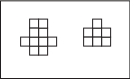
\includegraphics[width=0.5\linewidth]{images/SumPrinc}
\caption{The union of these two disjoint sets has size 17.\label{sumprinc}}
\end{figure}
\begin{figure}
\centering
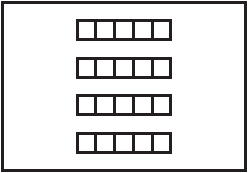
\includegraphics[width=0.5\linewidth]{images/ProdPrinc}
\caption{The union of four disjoint sets of size five.\label{prodprinc}}
\end{figure}
\hypertarget{p-78}{}%
You may have noticed some standard mathematical words and phrases such as \terminology{set}, \terminology{ordered pair}, \terminology{function} and so on creeping into the problems. One of our goals in these notes is to show how most counting problems can be recognized as counting all or some of the elements of a set of standard mathematical objects. For example \hyperref[orderedpair]{Problem~\ref{orderedpair}} is meant to suggest that the question we asked in \hyperref[basicsandwiches]{Problem~\ref{basicsandwiches}} was really a problem of counting all the ordered pairs consisting of a bread choice and a filling choice. We use \(A\times B\) to stand for the set of all ordered pairs whose first element is in \(A\) and whose second element is in \(B\) and we call \(A\times B\) the \index{Cartesian product}\index{product!Cartesian}\terminology{Cartesian product} of \(A\) and \(B\), so you can think of \hyperref[orderedpair]{Problem~\ref{orderedpair}} as asking you for the size of the Cartesian product of \(M\) and \(N\), that is, asking you to count the number of elements of this Cartesian product.%
\par
\hypertarget{p-79}{}%
When a set \(S\) is a union of disjoint sets \(B_1, B_2, \ldots, B_m\) we say that the sets \(B_1, B_2, \ldots, B_m\) are a \terminology{partition}\index{partition!of a set} of the set \(S\). Thus a partition of \(S\) is a (special kind of) set of sets. So that we don't find ourselves getting confused between the set \(S\) and the sets \(B_i\) into which we have divided it, we often call the sets \(B_1, B_2,
\ldots, B_m\) the \terminology{blocks}\index{partition!blocks of}\index{block of a partition} of the partition. In this language, the \index{principle!sum}\index{sum principle}\terminology{sum principle} says that%
\begin{quote}\hypertarget{blockquote-3}{}
\hypertarget{p-80}{}%
if we have a partition of a set \(S\), then the size of \(S\) is the sum of the sizes of the blocks of the partition.%
\end{quote}
\hypertarget{p-81}{}%
The \index{principle!product}\index{product principle}\terminology{product principle} says that%
\begin{quote}\hypertarget{blockquote-4}{}
\hypertarget{p-82}{}%
if we have a partition of a set \(S\) into \(m\) blocks, each of size \(n\), then \(S\) has size \(mn\).%
\end{quote}
\hypertarget{p-83}{}%
You'll notice that in our formal statement of the sum and product pinciple we talked about a partition of a finite set. We could modify our language a bit to cover infinite sizes, but whenever we talk about sizes of sets in what follows, we will be working with finite sets. So as to avoid possible complications in the future, let us agree that when we refer to the size of a set, we are implicitly assuming the set is finite. There is another version of the product principle that applies directly in problems like \hyperref[completelunch]{Problem~\ref{completelunch}} and \hyperref[tripledeckercone]{Problem~\ref{tripledeckercone}}, where we were not just taking a union of \(m\) disjoint sets of size \(n\), but rather \(m\) disjoint sets of size \(n\), each of which was a union of \(m'\) disjoint sets of size \(n'\). This is an inconvenient way to have to think about a counting problem, so we may rephrase the product principle in terms of a sequence of decisions:%
\begin{activity}[]\marginsymbol[-1em]{\pdftooltip{$\bullet$}{essential}} \label{generalproductprincipleintro}
\hypertarget{p-84}{}%
If we make a sequence of \(m\) choices for which \leavevmode%
\begin{itemize}[label=\textbullet]
\item{}there are \(k_1\) possible first choices, and%
\item{}for each way of making the first \(i-1\) choices, there are \(k_i\) ways to make the \(i\)th choice,%
\end{itemize}
 then in how many ways may we make our sequence of choices? (You need not prove your answer correct at this time.)%
\end{activity}
\hypertarget{p-85}{}%
The counting principle you gave in \hyperref[generalproductprincipleintro]{Problem~\ref{generalproductprincipleintro}} is called the \terminology{general product principle}.\index{general product principle}\index{product principle!general}\index{principle!product!general} We will outline a proof of the general product pinciple from the original product principle in \hyperref[generalproductprincipleproof]{Problem~\ref{generalproductprincipleproof}}. Until then, let us simply accept it as another counting principle. For now, notice how much easier it makes it to explain why we multiplied the things we did in \hyperref[completelunch]{Problem~\ref{completelunch}} and \hyperref[tripledeckercone]{Problem~\ref{tripledeckercone}}.%
\begin{activity}[]\marginsymbol[-1em]{\pdftooltip{$\importantarrow$}{especially interesting}} \label{tennispairings1}
\hypertarget{p-86}{}%
A tennis club has \(2n\) members. We want to pair up the members by twos for singles matches.%
\begin{enumerate}[font=\bfseries,label=(\alph*),ref=\alph*]
\item\label{tennispairings1a} \marginsymbol[-2.5em]{} \hypertarget{p-87}{}%
In how many ways may we pair up all the members of the club? (Hint: consider the cases of 2, 4, and 6 members.)%
~{\tiny (h)}\item\label{task-14} \marginsymbol[-2.5em]{} \hypertarget{p-90}{}%
Suppose that in addition to specifying who plays whom, for each pairing we say who serves first.  Now in how many ways may we specify our pairs?%
\end{enumerate}
\end{activity}
\begin{activity}[]\marginsymbol[-1em]{\pdftooltip{\tiny$+$}{summary}} \label{countingfunctions2}
\hypertarget{p-91}{}%
Let us now return to \hyperref[countingfunctions]{Problem~\ref{countingfunctions}} and justify\textemdash{}or perhaps finish\textemdash{}our answer to the question about the number of functions from a three-element set to a 12-element set.%
\begin{enumerate}[font=\bfseries,label=(\alph*),ref=\alph*]
\item\label{task-15} \marginsymbol[-2.5em]{} \hypertarget{p-92}{}%
How can you justify your answer in \hyperref[countingfunctions]{Problem~\ref{countingfunctions}} to the question ``How many functions are there from a three element set (say \([3]=\{1,2,3\}\)) to a twelve element set (say [12])?''%
\item\label{numberoffunctionsconjecture} \marginsymbol[-2.5em]{} \hypertarget{p-94}{}%
Based on the examples you've seen so far, make a conjecture about how many functions there are from the set%
\begin{equation*}
[m] = \{1,2,3,\dots,m\}
\end{equation*}
to \([n]=\{1,2,3,\dots,n\}\) and prove it.%
\item\label{task-17} \marginsymbol[-2.5em]{} \hypertarget{p-96}{}%
A common notation for the set of all functions from a set \(M\) to a set \(N\) is \(N^M\).  Why is this a good notation?%
\end{enumerate}
\end{activity}
\begin{activity}[]\marginsymbol[-1em]{\pdftooltip{\tiny$+$}{summary}} \label{generalproductprinciple}
\hypertarget{p-98}{}%
Now suppose we are thinking about a set \(S\) of functions \(f\) from \([m]\) to some set \(X\). (For example, in \hyperref[tripledeckercone]{Problem~\ref{tripledeckercone}} we were thinking of the set of functions from the three possible places for scoops in an ice-cream cone to \(12\) flavors of ice cream.) Suppose there are \(k_1\) choices for \(f(1)\). (In \hyperref[tripledeckercone]{Problem~\ref{tripledeckercone}}, \(k_1\) was \(12\), because there were \(12\) ways to choose the first scoop.) Suppose that for each choice of \(f(1)\) there are \(k_2\) choices for \(f(2)\). (For example, in \hyperref[tripledeckercone]{Problem~\ref{tripledeckercone}} \(k_2\) was \(12\) if the second flavor could be the same as the first, but \(k_2\) was \(11\) if the flavors had to be different.) In general, suppose that for each choice of \(f(1)\), \(f(2)\), \textellipsis{} \(f(i-1)\), there are \(k_i\) choices for \(f(i)\). (For example, in \hyperref[tripledeckercone]{Problem~\ref{tripledeckercone}}, if the flavors have to be different, then for each choice of \(f(1)\) and \(f(2)\), there are \(10\) choices for \(f(3)\).)%
\par
\hypertarget{p-99}{}%
What we have assumed so far about the functions in \(S\) may be summarized as \leavevmode%
\begin{itemize}[label=\textbullet]
\item{}There are \(k_1\) choices for \(f(1)\).%
\item{}For each choice of \(f(1)\), \(f(2)\), \textellipsis{}, \(f(i-1)\), there are \(k_i\) choices for~\(f(i)\).%
\end{itemize}
%
\par
\hypertarget{p-100}{}%
How many functions are in the set \(S\)? Is there any practical difference between the result of this problem and the general product principle?%
\end{activity}
\hypertarget{p-102}{}%
The point of \hyperref[generalproductprinciple]{Problem~\ref{generalproductprinciple}} is that the general product principle can be stated informally, as we did originally, or as a statement about counting sets of standard concrete mathematical objects, namely functions.%
\begin{activity}[]\marginsymbol[-1em]{\pdftooltip{$\importantarrow$}{especially interesting}} \label{activity-15}
\hypertarget{p-103}{}%
A roller coaster car has \(n\) rows of seats, each of which has room for two people. If \(n\) men and \(n\) women get into the car with a man and a woman in each row, in how many ways may they choose their seats?%
~{\tiny (h)}\end{activity}
\begin{activity}[]\marginsymbol[-1em]{\pdftooltip{\tiny$+$}{summary}} \label{activity-16}
\hypertarget{p-106}{}%
How does the general product principle apply to \hyperref[tripledeckercone]{Problem~\ref{tripledeckercone}}?%
\end{activity}
\begin{activity}[]\marginsymbol[-1em]{\pdftooltip{$\bullet$}{essential}} \label{activity-17}
\hypertarget{p-108}{}%
In how many ways can we pass out \(k\) distinct pieces of fruit to \(n\) children (with no restriction on how many pieces of fruit a child may get)?%
\end{activity}
\begin{activity}[]\marginsymbol[-1em]{\pdftooltip{$\bullet$}{essential}} \label{SubsetsFirstTime}
\hypertarget{p-110}{}%
How many subsets does a set \(S\) with \(n\) elements have?%
~{\tiny (h)}\end{activity}
\begin{activity}[]\marginsymbol[-1em]{\pdftooltip{$\circ$}{motivational material}} \label{activity-19}
\hypertarget{p-113}{}%
Assuming \(k\le n\), in how many ways can we pass out \(k\) distinct pieces of fruit to \(n\) children if each child may get at most one? What is the number if \(k>n\)? Assume for both questions that we pass out all the fruit.%
~{\tiny (h)}~{\tiny (h)}\end{activity}
\begin{activity}[]\marginsymbol[-1em]{\pdftooltip{$\bullet$}{essential}} \label{kelementpermutation}
\hypertarget{p-117}{}%
Another name for a list, in a specific order, of \(k\) distinct things chosen from a set \(S\) is a \terminology{\(k\)-element permutation} of \(S\).\index{permutation!\(k\)-element} We can also think of a \(k\)-element permutation of \(S\) as a one-to-one function (or, in other words, injection) from \([k]=\{1,2,\ldots, k\}\) to \(S\). How many \(k\)-element permutations does an \(n\)-element set have? (For this problem it is natural to assume \(k\le n\). However the question makes sense even if \(k>n\). What is the number of \(k\)-element permutations of an \(n\)-element set if \(k>n\)?%
~{\tiny (h)}\end{activity}
\hypertarget{p-120}{}%
There are a number of different notations for the number of \(k\)-element permutations of an \(n\)-element set. The one we shall use was introduced by Don Knuth; namely \(n^{\underline{k}}\), read ``\(n\) to the \(k\) falling'' or ``\(n\) to the \(k\) down''. In \hyperref[kelementpermutation]{Problem~\ref{kelementpermutation}} you may have shown that%
\begin{equation}
n^{\underline{k}} =n(n-1)\cdots (n-k+1)= \prod_{i=1}^k(
n-i+1).\label{productnotation}
\end{equation}
%
\par
\hypertarget{p-121}{}%
It is standard to call \(n^{\underline{k}}\)\index{\(n^{\underline{k}}\)} the \terminology{\(k\)-th falling factorial power of \(n\)}\index{falling factorial power}\index{factorial power!falling}, which explains why we use exponential notation. Of course we call it a \terminology{factorial} power since \(n^{\underline{n}} = n(n-1)\cdots 1\) which we call \terminology{\(n\)-factorial} and denote by \(n!\).\index{factorial}\index{\(n"!\)} If you are unfamiliar with the \(\Pi\) notation, or \terminology{product notation}\index{product notation}\index{\(\Pi\) notation} we introduced for products in \hyperref[productnotation]{Equation~(\ref{productnotation})}, it works just like the \(\Sigma\) notation works for summations.%
\begin{activity}[]\marginsymbol[-1em]{\pdftooltip{$\bullet$}{essential}} \label{activity-21}
\hypertarget{p-122}{}%
Express \(n^{\underline{k}}\) as a quotient of factorials.%
\end{activity}
\begin{activity}[]\marginsymbol[-1em]{\pdftooltip{$\importantarrow$}{especially interesting}} \label{activity-22}
\hypertarget{p-124}{}%
How should we define \(n^{\underline{0}}\)?%
\end{activity}
\typeout{************************************************}
\typeout{Subsection 1.2.2 Functions and directed graphs}
\typeout{************************************************}
\subsection[{Functions and directed graphs}]{Functions and directed graphs}\label{subsection-2}
\hypertarget{p-126}{}%
As another example how standard mathematical language relates to counting problems, \hyperref[countingfunctions]{Problem~\ref{countingfunctions}} explicitly asked you to relate the idea of counting functions to the question of \hyperref[tripledeckercone]{Problem~\ref{tripledeckercone}}. You have probably learned in algebra or calculus how to draw graphs in the Cartesian plane of functions from a set of numbers to a set of numbers. You may recall how we can determine whether a graph is a graph of a function by examining whether each vertical straight line crosses the graph at most one time. You might also recall how we can determine whether such a function is one-to-one by examining whether each horizontal straight line crosses the graph at most one time. The functions we deal with will often involve objects which are not numbers, and will often be functions from one finite set to another. Thus graphs in the cartesian plane will often not be available to us for visualizing functions.%
\par
\hypertarget{p-127}{}%
However, there is another kind of graph called a \terminology{directed graph}\index{graph!directed}\index{directed graph} or \terminology{digraph}\index{digraph}\index{function!digraph of} that is especially useful when dealing with functions between finite sets. We take up this topic in more detail in \hyperref[Relations]{Appendix~\ref{Relations}}, particularly \hyperref[relationdigraph]{Subsection~\ref{relationdigraph}} and \hyperref[digraphsoffunctions]{Subsection~\ref{digraphsoffunctions}}. In \hyperref[functiondigraphs]{Figure~\ref{functiondigraphs}} we show several examples of digraphs of functions.%
\begin{figure}
\centering
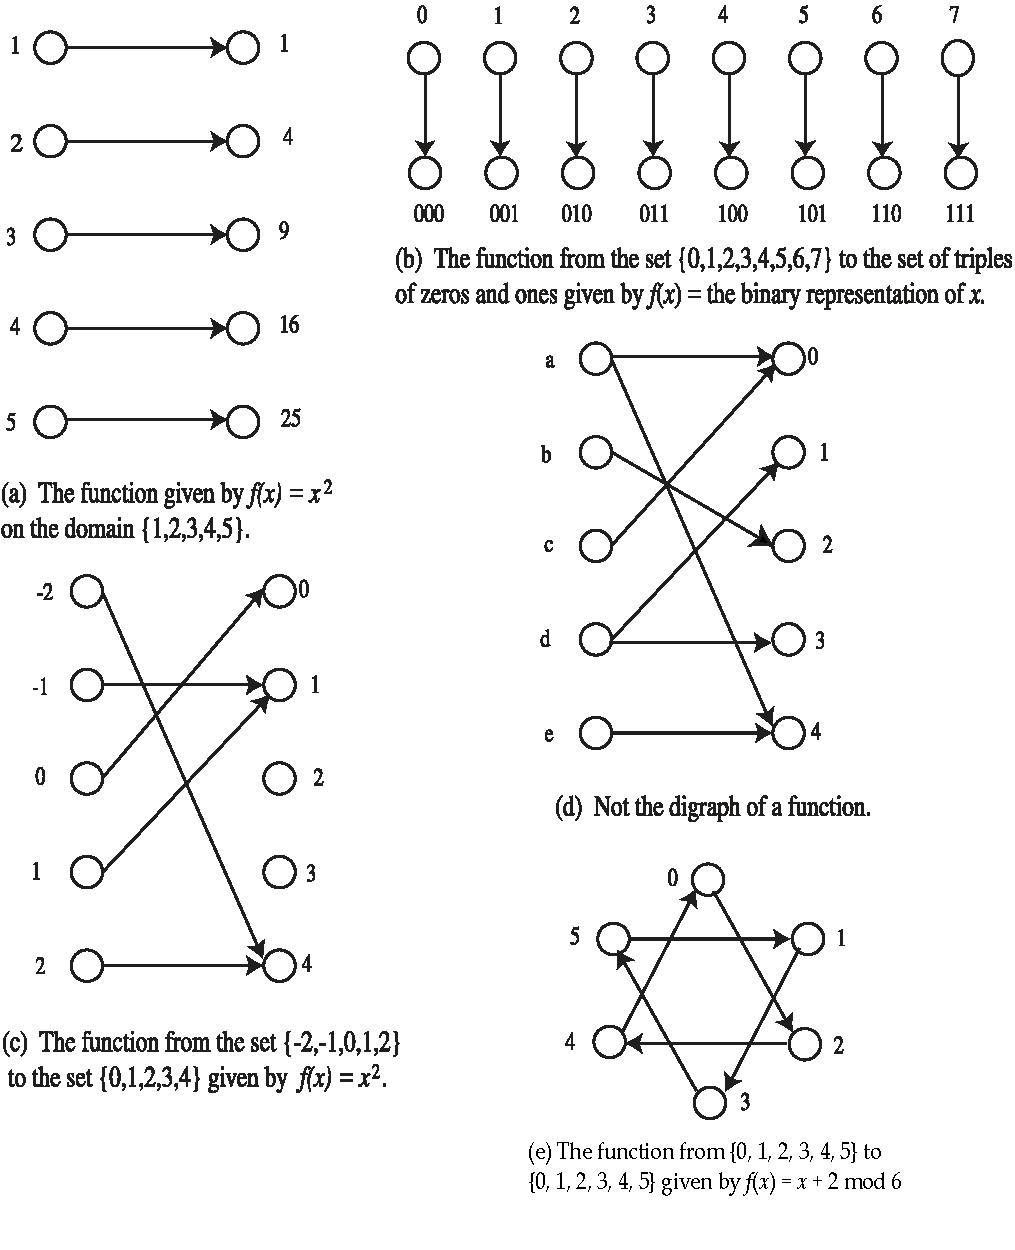
\includegraphics[width=0.73\linewidth]{images/functiondigraph}
\caption{What is a digraph of a function?\label{functiondigraphs}}
\end{figure}
\hypertarget{p-128}{}%
If we have a function \(f\) from a set \(S\) to a set \(T\), we draw a line of dots or circles, called \terminology{vertices} to represent the elements of \(S\) and another (usually parallel) line of circles or dots to represent the elements of \(T\). We then draw an arrow from the circle for \(x\) to the circle for \(y\) if \(f(x) = y\). Sometimes, as in part (e) of the figure, if we have a function from a set \(S\) to itself, we draw only one set of vertices representing the elements of \(S\), in which case we can have arrows both entering and leaving a given vertex. As you see, the digraph can be more enlightening in this case if we experiment with the function to find a nice placement of the vertices rather than putting them in a row.%
\par
\hypertarget{p-129}{}%
Notice that there is a simple test for whether a digraph whose vertices represent the elements of the sets \(S\) and \(T\) is the digraph of a function from \(S\) to \(T\). There must be one and only one arrow leaving each vertex of the digraph representing an element of \(S\). The fact that there is one arrow means that \(f(x)\) is defined for each \(x\) in \(S\). The fact that there is only one arrow means that each \(x\) in \(S\) is related to exactly one element of \(T\). (Note that these remarks hold as well if we have a function from \(S\) to \(S\) and draw only one set of vertices representing the elements of \(S\).) For further discussion of functions and digraphs see \hyperref[functionrelation]{Sections~\ref{functionrelation}} and \hyperref[relationdigraph]{Subsection~\ref{relationdigraph}} of {\hyperref[Relations]{Appendix~\ref{Relations}}}.%
\begin{activity}[]\marginsymbol[-1em]{\pdftooltip{$\circ$}{motivational material}} \label{activity-23}
\hypertarget{p-130}{}%
Draw the digraph of the function from the set \(\{\)Alice, Bob, Dawn, Bill\(\}\) to the set \(\{\)A, B, C, D, E\(\}\) given by%
\begin{equation*}
f(X) = \text{ the first letter of the name }X .
\end{equation*}
%
\end{activity}
\begin{activity}[]\marginsymbol[-1em]{\pdftooltip{$\bullet$}{essential}} \label{activity-24}
\hypertarget{p-131}{}%
A function \(f:S\rightarrow T\) is called an \index{onto function}\index{function!onto}\terminology{onto function} or \index{surjection}\index{function!surjection}\terminology{surjection} if each element of \(T\) is \(f(x)\) for some \(x\in S\). Choose a set \(S\) and a set \(T\) so that you can draw the digraph of a function from \(S\) to \(T\) that is one-to-one but not onto, and draw the digraph of such a function.%
\end{activity}
\begin{activity}[]\marginsymbol[-1em]{\pdftooltip{$\circ$}{motivational material}} \label{activity-25}
\hypertarget{p-133}{}%
Choose a set \(S\) and a set \(T\) so that you can draw the digraph of a function from \(S\) to \(T\) that is onto but not one-to-one, and draw the digraph of such a function.%
\end{activity}
\begin{activity}[]\marginsymbol[-1em]{\pdftooltip{$\bullet$}{essential}} \label{activity-26}
\hypertarget{p-135}{}%
Digraphs of functions help us visualize the ideas of one-to-one functions and onto functions.%
\begin{enumerate}[font=\bfseries,label=(\alph*),ref=\alph*]
\item\label{task-18} \marginsymbol[-2.5em]{} \hypertarget{p-136}{}%
What does the digraph of a one-to-one function (injection) from a finite set \(X\) to a finite set \(Y\) look like? (Look for a test somewhat similar to the one we described for when a digraph is the digraph of a function.)%
~{\tiny (h)}\item\label{task-19} \marginsymbol[-2.5em]{} \hypertarget{p-139}{}%
What does the digraph of an onto function look like?%
\item\label{bijectiondigraph} \marginsymbol[-2.5em]{} \hypertarget{p-141}{}%
What does the digraph of a one-to-one and onto function from a finite set \(S\) to a set \(T\) look like?%
\end{enumerate}
\end{activity}
\begin{activity}[]\marginsymbol[-1em]{\pdftooltip{$\bullet$}{essential}} \label{permutationasbijection}
\hypertarget{p-143}{}%
The word \emph{permutation} is actually used in two different ways in mathematics. A \terminology{permutation}\index{permutation!as a bijection} of a set \(S\) is one-to-one from \(S\) onto \(S\). How many permutations does an \(n\)-element set have?%
\end{activity}
\hypertarget{p-145}{}%
Notice that there is a great deal of consistency between the use of the word permutation in \hyperref[permutationasbijection]{Problem~\ref{permutationasbijection}} and the use in \hyperref[kelementpermutation]{Problem~\ref{kelementpermutation}}. If we have some way \(a_1,a_2,\ldots,a_n\) of listing our set, then any other list \(b_1,b_2,\ldots,b_n\) gives us the permutation of \(S\) whose rule is \(f(a_i) =b_i\), and any permutation of \(S\), say the one given by \(g(a_i)=c_i\) gives us a list \(c_1,c_2,\ldots,c_n\) of \(S\). Thus there is really very little difference between the idea of a permutation of \(S\) and an \(n\)-element permutation of \(S\) when \(n\) is the size of \(S\).%
\typeout{************************************************}
\typeout{Subsection 1.2.3 The bijection principle}
\typeout{************************************************}
\subsection[{The bijection principle}]{The bijection principle}\label{subsection-3}
\hypertarget{p-146}{}%
Another name for a one-to-one and onto function is \index{bijection}\index{function!bijection}\terminology{bijection}. The digraphs marked (a), (b), and (e) in \hyperref[functiondigraphs]{Figure~\ref{functiondigraphs}} are digraphs of bijections. The description in \hyperref[bijectiondigraph]{Problem~\ref{activity-26}.\ref{bijectiondigraph}} of the digraph of a bijection from \(X\) to \(Y\) illustrates one of the fundamental principles of combinatorial mathematics, the \index{principle!bijection}\index{bijection principle}\terminology{bijection principle}:%
\begin{quote}\hypertarget{blockquote-5}{}
\hypertarget{p-147}{}%
Two sets have the same size if and only if there is a bijection between them.%
\end{quote}
\hypertarget{p-148}{}%
It is surprising how this innocent sounding principle guides us into finding insight into some otherwise very complicated proofs.%
\typeout{************************************************}
\typeout{Subsection 1.2.4 Counting subsets of a set}
\typeout{************************************************}
\subsection[{Counting subsets of a set}]{Counting subsets of a set}\label{subsection-4}
\begin{activity}[]\marginsymbol[-1em]{} \label{SubsetsBinaryRepresentation}
\hypertarget{p-149}{}%
The \terminology{binary representation} of a number \(m\) is a list, or string, \(a_1a_2\ldots a_k\) of zeros and ones such that \(m=a_12^{k-1} + a_2 2^{k-2}
+\cdots+ a_k 2^0.\) Describe a bijection between the binary representations of the integers between 0 and \(2^n-1\) and the subsets of an \(n\)-element set. What does this tell you about the number of subsets of an \(n\)-element set?%
~{\tiny (h)}\end{activity}
\hypertarget{p-152}{}%
Notice that the first question in \hyperref[icecreaminpints]{Problem~\ref{icecreaminpints}} asked you for the number of ways to choose a three element subset from a 12 element subset. You may have seen a notation like \(\binom{n}{k}\), \(C(n,k)\), or \(_nC_k\) which stands for the number of ways to choose a \(k\)-element subset from an \(n\)-element set. The number \(\binom{n}{k}\) is read as ``\(n\) choose \(k\)'' and is called a \index{binomial coefficient}\terminology{binomial coefficient} for reasons we will see later on. Another frequently used way to read the binomial coefficient notation is ``the number of combinations \index{combinations} of \(n\) things taken \(k\) at a time." You are going to be asked to construct two bijections that relate to these numbers and figure out what famous formula they prove. We are going to think about subsets of the \(n\)-element set \([n] =
\{1,2,3,\ldots, n\}\). As an example, the set of two-element subsets of \([4]\) is%
\begin{equation*}
\{\{1,2\}, \{1,3\}, \{1,4\}, \{2,3\}, \{2,4\}, \{3,4\}\}.
\end{equation*}
%
\par
\hypertarget{p-153}{}%
This example tells us that \(\binom{4}{2} = 6\).%
\begin{activity}[]\marginsymbol[-1em]{\pdftooltip{$\bullet$}{essential}} \label{Pascal}
\hypertarget{p-154}{}%
Let \(C\) be the set of \(k\)-element subsets of \([n]\) that contain the number \(n\), and let \(D\) be the set of \(k\)-element subsets of \([n]\) that don't contain \(n\).%
\begin{enumerate}[font=\bfseries,label=(\alph*),ref=\alph*]
\item\label{task-21} \marginsymbol[-2.5em]{} \hypertarget{p-155}{}%
Let \(C'\) be the set of \((k-1)\)-element subsets of \([n-1]\).  Describe a bijection from \(C\) to \(C'\).  (A verbal description is fine.)%
\item\label{task-22} \marginsymbol[-2.5em]{} \hypertarget{p-157}{}%
Let \(D'\) be the set of \(k\)-element subsets of \([n-1]=\{1,2,\ldots n-1\}\).  Describe a bijection from \(D\) to \(D'\). (A verbal description is fine.)%
\item\label{task-23} \marginsymbol[-2.5em]{} \hypertarget{p-159}{}%
Based on the two previous parts, express the sizes of \(C\) and \(D\) in terms of binomial coefficients involving \(n-1\) instead of \(n\).%
\item\label{task-24} \marginsymbol[-2.5em]{} \hypertarget{p-161}{}%
Apply the sum principle to \(C\) and \(D\) and obtain a formula that expresses \(\binom{n}{k}\) in terms of two binomial coefficients involving \(n-1\).  You have just derived the Pascal Equation that is the basis for the famous Pascal's Triangle.%
\end{enumerate}
\end{activity}
\typeout{************************************************}
\typeout{Subsection 1.2.5 Pascal's Triangle}
\typeout{************************************************}
\subsection[{Pascal's Triangle}]{Pascal's Triangle}\label{subsection-5}
\hypertarget{p-163}{}%
The Pascal Equation that you derived in \hyperref[Pascal]{Problem~\ref{Pascal}} gives us the triangle in \hyperref[Pascaltriangle]{Figure~\ref{Pascaltriangle}}. This figure has the number of \(k\)-element subsets of an \(n\)-element set as the \(k\)th number over in the \(n\)th row (we call the top row the zeroth row and the beginning entry of a row the zeroth number over). You'll see that your formula doesn't say anything about \(\binom{n}{k}\) if \(k=0\) or \(k=n\), but otherwise it says that each entry is the sum of the two that are above it and just to the left or right.%
\begin{figure}
\centering
% group protects changes to lengths, releases boxes (?)
{% begin: group for a single side-by-side
% set panel max height to practical minimum, created in preamble
\setlength{\panelmax}{0pt}
\ifdefined\panelboxAp\else\newsavebox{\panelboxAp}\fi%
\savebox{\panelboxAp}{%
\raisebox{\depth}{\parbox{1\linewidth}{%
\begin{equation*}
\begin{matrix}\amp \amp \amp \amp \amp \amp \amp 1\amp \amp \amp \amp \amp \amp \amp \\
\amp \amp \amp \amp \amp \amp 1\amp \amp 1\amp \amp \amp \amp \amp \amp \\
\amp \amp \amp \amp \amp 1\amp \amp 2\amp \amp 1\amp \amp \amp \amp \amp \\
\amp \amp \amp \amp 1\amp \amp 3\amp \amp 3\amp \amp 1\amp \amp \amp \amp \\
\amp \amp \amp 1\amp \amp 4\amp \amp 6\amp \amp 4\amp \amp 1\amp \amp \\
\amp \amp 1\amp \amp 5\amp \amp 10\amp \amp 10\amp \amp 5\amp \amp 1\amp \\
\amp 1\amp \amp 6\amp \amp 15\amp \amp 20\amp \amp 15\amp \amp 6\amp \amp 1\\
1\amp \amp 7\amp \amp 21\amp \amp 35\amp \amp 35\amp \amp 21\amp \amp 7\amp \amp 1
\end{matrix}
\end{equation*}
}}}
\ifdefined\phAp\else\newlength{\phAp}\fi%
\setlength{\phAp}{\ht\panelboxAp+\dp\panelboxAp}
\settototalheight{\phAp}{\usebox{\panelboxAp}}
\setlength{\panelmax}{\maxof{\panelmax}{\phAp}}
\leavevmode%
% begin: side-by-side as tabular
% \tabcolsep change local to group
\setlength{\tabcolsep}{0\linewidth}
% @{} suppress \tabcolsep at extremes, so margins behave as intended
\par\medskip\noindent
\begin{tabular}{@{}*{1}{c}@{}}
\begin{minipage}[c][\panelmax][t]{1\linewidth}\usebox{\panelboxAp}\end{minipage}\end{tabular}\\
% end: side-by-side as tabular
}% end: group for a single side-by-side
\caption{Pascal's Triangle\label{Pascaltriangle}}
\end{figure}
\hypertarget{p-165}{}%
\index{Pascal's Triangle}%
\begin{activity}[]\marginsymbol[-1em]{} \label{activity-30}
\hypertarget{p-166}{}%
Just for practice, what is the next row of Pascal's triangle?%
\end{activity}
\begin{activity}[]\marginsymbol[-1em]{\pdftooltip{$\importantarrow$}{especially interesting}} \label{activity-31}
\hypertarget{p-168}{}%
Without writing out the rows completely, write out enough of Pascal's triangle to get a numerical answer for the first question in \hyperref[icecreaminpints]{Problem~\ref{icecreaminpints}}.%
~{\tiny (h)}\end{activity}
\hypertarget{p-171}{}%
It is less common to see Pascal's triangle as a right triangle, but it actually makes your formula easier to interpret. In Pascal's Right Triangle, the element in row \(n\) and column \(k\) (with the convention that the first row is row zero and the first column is column zero) is \(\binom{n}{k}\). In this case your formula says each entry in a row is the sum of the one above and the one above and to the left, except for the leftmost and rightmost entries of a row, for which that doesn't make sense. Since the leftmost entry is \(\binom{n}{0}\) and the rightmost entry is \(\binom{n}{n}\), these entries are both one (to see why, ask yourself how many \(0\)-element subsets and how many \(n\)-element subsets an \(n\)-element set has), and your formula then tells how to fill in the rest of the table.%
\begin{table}
\centering
\begin{tabular}{cArrrrrrrr}
\multicolumn{2}{r}{\(k=0\)}&1&2&3&4&5&6&7\tabularnewline\hrulethin
\(n=0\)&1&&&&&&\tabularnewline[0pt]
1&1&1&&&&&\tabularnewline[0pt]
2&1&2&1&&&&&\tabularnewline[0pt]
3&1&3&3&1&&&&\tabularnewline[0pt]
4&1&4&6&4&1&&&\tabularnewline[0pt]
5&1&5&10&10&5&1&&\tabularnewline[0pt]
6&1&6&15&20&15&6&1&\tabularnewline[0pt]
7&1&7&21&35&35&21&7&1
\end{tabular}
\caption{Pascal's Right Triangle\label{Pascalrighttriangle}}
\end{table}
\hypertarget{p-172}{}%
Seeing this right triangle leads us to ask whether there is some natural way to extend the right triangle to a rectangle. If we did have a rectangular table of binomial coefficients, counting the first row as row zero (i.e., \(n=0\)) and the first column as column zero (i.e., \(k=0\)), the entries we don't yet have are values of \(\binom{n}{k}\) for \(k>n\). But how many \(k\)-element subsets does an \(n\)-element set have if \(k>n\)? The answer, of course, is zero, so all the other entries we would fill in would be zero, giving us the rectangular array in \hyperref[Pascal_sRectangle]{Figure~\ref{Pascal_sRectangle}}. It is straightforward to check that Pascal's equation now works for all the entries in the rectangle that have an entry above them and an entry above and to the left.%
\begin{table}
\centering
\begin{tabular}{cArrrrrrrr}
\multicolumn{2}{r}{\(k=0\)}&1&2&3&4&5&6&7\tabularnewline\hrulethin
\(n=0\)&1&0&0&0&0&0&0&0\tabularnewline[0pt]
1&1&1&0&0&0&0&0&0\tabularnewline[0pt]
2&1&2&1&0&0&0&0&0\tabularnewline[0pt]
3&1&3&3&1&0&0&0&0\tabularnewline[0pt]
4&1&4&6&4&1&0&0&0\tabularnewline[0pt]
5&1&5&10&10&5&1&0&0\tabularnewline[0pt]
6&1&6&15&20&15&6&1&0\tabularnewline[0pt]
7&1&7&21&35&35&21&7&1
\end{tabular}
\caption{Pascal's Rectangle\label{Pascal_sRectangle}}
\end{table}
\begin{activity}[]\marginsymbol[-1em]{\pdftooltip{$\importantarrow$}{especially interesting}} \label{activity-32}
\hypertarget{p-173}{}%
Because our definition told us that \(\binom{n}{k}\) is 0 when \(k>n\), we got a rectangular table of numbers that satisfies the Pascal Equation.%
\begin{enumerate}[font=\bfseries,label=(\alph*),ref=\alph*]
\item\label{task-25} \marginsymbol[-2.5em]{} \hypertarget{p-174}{}%
Is there any other way to define \(\binom{n }{k}\) when \(k>n\) in order to get a rectangular table that agrees with Pascal's Right Triangle for \(k\le n\) and satisfies the Pascal Equation?%
~{\tiny (h)}\item\label{task-26} \marginsymbol[-2.5em]{} \hypertarget{p-177}{}%
Suppose we want to extend Pascal's Rectangle to the left and define \(\binom{n}{-k}\) for \(n\ge 0\) and \(k>0\) so that \(-k\lt 0\). What should we put into row \(n\) and column \(-k\) of Pascal's Rectangle in order for the Pascal Equation to hold true?%
~{\tiny (h)}\item\label{task-27} \marginsymbol[-2.5em]{} \hypertarget{p-180}{}%
What should we put into row \(-n\) and column \(k\) or column \(-k\) in order for the Pascal Equation to continue to hold?  Do we have any freedom of choice?%
~{\tiny (h)}\end{enumerate}
\end{activity}
\begin{activity}[]\marginsymbol[-1em]{} \label{charfunction}
\hypertarget{p-183}{}%
There is yet another bijection that lets us prove that a set of size \(n\) has \(2^n\) subsets. Namely, for each subset \(S\) of \([n]=\{1,2,\ldots, n\}\), define a function (traditionally denoted by \(\chi_S\)) as follows.\footnote{The symbol \(\chi\) is the Greek letter chi that is pronounced Ki, with the \(i\) sounding like ``eye.''\label{fn-1}}%
\begin{equation*}
\chi_S(i) = \begin{cases}1 \amp \text{ if }  i\in S \\ 0 \amp \text{ if }  i\not\in
S
\end{cases}
\end{equation*}
%
\par
\hypertarget{p-184}{}%
The function \(\chi_S\) is called the \index{characteristic function}\index{function!characteristic}\terminology{characteristic function} of \(S\). Notice that the characteristic function is a function from \([n]\) to \(\{0,1\}\).%
\begin{enumerate}[font=\bfseries,label=(\alph*),ref=\alph*]
\item\label{task-28} \marginsymbol[-2.5em]{} \hypertarget{p-185}{}%
For practice, consider the function \(\chi_{\{1,3\}}\) for the subset \(\{1,3\}\) of the set \(\{1,2,3,4\}\).  What are%
\begin{enumerate}[font=\bfseries,label=(\roman*),ref=\theenumi.\roman*]
\item\label{task-29} \marginsymbol[-2.5em]{} \hypertarget{p-186}{}%
\(\chi_{\{1,3\}}(1)\)?%
\item\label{task-30} \marginsymbol[-2.5em]{} \hypertarget{p-188}{}%
\(\chi_{\{1,3\}}(2)\)?%
\item\label{task-31} \marginsymbol[-2.5em]{} \hypertarget{p-190}{}%
\(\chi_{\{1,3\}}(3)\)?%
\item\label{task-32} \marginsymbol[-2.5em]{} \hypertarget{p-192}{}%
\(\chi_{\{1,3\}}(4)\)?%
\end{enumerate}
\item\label{task-33} \marginsymbol[-2.5em]{} \hypertarget{p-194}{}%
We define a function \(f\) from the set of subsets of \([n]=\{1,2,\ldots, n\}\) to the set of functions from \([n]\) to \(\{0,1\}\) by \(f(S)=\chi_S\).  Explain why \(f\) is a bijection.%
\item\label{task-34} \marginsymbol[-2.5em]{} \hypertarget{p-196}{}%
Why does the fact that \(f\) is a bijection prove that \([n]\) has \(2^n\) subsets?%
\end{enumerate}
\end{activity}
\hypertarget{p-198}{}%
In \hyperref[SubsetsFirstTime]{Problems~\ref{SubsetsFirstTime}}, \hyperref[SubsetsBinaryRepresentation]{Problem~\ref{SubsetsBinaryRepresentation}}, and \hyperref[charfunction]{Problem~\ref{charfunction}} you gave three proofs of the following theorem.%
\begin{theorem}[{}]\label{theorem-1}
\hypertarget{p-199}{}%
The number of subsets of an \(n\)-element set is \(2^n\).%
\end{theorem}
\hypertarget{p-200}{}%
The proofs in \hyperref[SubsetsBinaryRepresentation]{Problem~\ref{SubsetsBinaryRepresentation}} and \hyperref[charfunction]{Problem~\ref{charfunction}} use essentially the same bijection, but they interpret sequences of zeros and ones differently, and so end up being different proofs. We will give yet another proof, using bijections similar to those we used in proving the Pascal Equation, at the beginning of \hyperref[InductionRecursion]{Chapter~\ref{InductionRecursion}}.%
\typeout{************************************************}
\typeout{Subsection 1.2.6 The quotient principle}
\typeout{************************************************}
\subsection[{The quotient principle}]{The quotient principle}\label{subsection-6}
\begin{activity}[]\marginsymbol[-1em]{\pdftooltip{$\bullet$}{essential}} \label{twelvechoosethree}
\hypertarget{p-201}{}%
As we noted in \hyperref[Pascal]{Problem~\ref{Pascal}}, the first question in \hyperref[icecreaminpints]{Problem~\ref{icecreaminpints}} asked us for the number of three-element subsets of a twelve-element set. We were able to use the Pascal Equation to get a numerical answer to that question. Had we had twenty or thirty flavors of ice cream to choose from, using the Pascal Equation to get our answer would have entailed a good bit more work. We have seen how the general product principle gives us an answer to \hyperref[tripledeckercone]{Problem~\ref{tripledeckercone}}. Thus we might think that the number of ways to choose a three element set from 12 elements is the number of ways to choose the first element times the number of ways to choose the second element times the number of ways to choose the third element, which is \(12\cdot11\cdot10=1320\). However, our result in \hyperref[Pascal]{Problem~\ref{Pascal}} shows that this is wrong.%
\begin{enumerate}[font=\bfseries,label=(\alph*),ref=\alph*]
\item\label{task-35} \marginsymbol[-2.5em]{} \hypertarget{p-202}{}%
What is it that is different between the number of ways to stack ice cream in a triple decker cone with three different flavors of ice cream and the number of ways to simply choose three different flavors of ice cream?%
\item\label{twelvechoosethreethree} \marginsymbol[-2.5em]{} \hypertarget{p-204}{}%
In particular, how many different triple decker cones use the same three flavors?  (Of course any three distinct flavors could substitute for vanilla, chocolate and strawberry without changing the answer.)%
\item\label{twelvechoosethreefinal} \marginsymbol[-2.5em]{} \hypertarget{p-206}{}%
Using your answer from \hyperref[twelvechoosethreethree]{part~b}, compute the number of ways to choose three different flavors of ice cream (out of twelve flavors) from the number of ways to choose a triple decker cone with three different flavors (out of twelve  flavors).%
\end{enumerate}
\end{activity}
\begin{activity}[]\marginsymbol[-1em]{\pdftooltip{$\bullet$}{essential}} \label{nchoosek}
\hypertarget{p-208}{}%
Based on what you observed in \hyperref[twelvechoosethreefinal]{Problem~\ref{twelvechoosethree}.\ref{twelvechoosethreefinal}}, how many \(k\)-element subsets does an \(n\)-element set have?%
\end{activity}
\begin{activity}[]\marginsymbol[-1em]{\pdftooltip{$\importantarrow$}{especially interesting}} \label{activity-36}
\hypertarget{p-210}{}%
The formula you proved in \hyperref[nchoosek]{Problem~\ref{nchoosek}} is symmetric in \(k\) and \(n-k\); that is, it gives the same number for \(\binom{n}{k}\) as it gives for \(\binom{n}{n-k}\). Whenever two quantities are counted by the same formula it is good for our insight to find a bijection that demonstrates the two sets being counted have the same size. In fact this is a guiding principle of research in combinatorial mathematics. Find a bijection that proves that \(\binom{n}{k}\) equals \(\binom{n}{n-k}\).%
~{\tiny (h)}\end{activity}
\begin{activity}[]\marginsymbol[-1em]{\pdftooltip{$\bullet$}{essential}} \label{ping-pong}
\hypertarget{p-213}{}%
In how many ways can we pass out \(k\) (identical) ping-pong balls to \(n\) children if each child may get at most one?%
~{\tiny (h)}\end{activity}
\begin{activity}[]\marginsymbol[-1em]{\pdftooltip{$\bullet$}{essential}} \label{roundtable}
\hypertarget{p-216}{}%
In how many ways may \(n\) people sit around a round table? (Assume that when people are sitting around a round table, all that really matters is who is to each person's right. For example, if we can get one arrangement of people around the table from another by having everyone get up and move to the right one place and sit back down, we get an equivalent arrangement of people. Notice that you can get a list from a seating arrangement by marking a place at the table, and then listing the people at the table, starting at that place and moving around to the right.) There are at least two different ways of doing this problem. Try to find them both.%
~{\tiny (h)}~{\tiny (h)}\end{activity}
\hypertarget{p-220}{}%
We are now going to analyze the result of \hyperref[nchoosek]{Problem~\ref{nchoosek}} in more detail in order to tease out another counting principle that we can use in a wide variety of situations.%
\begin{table}
\centering
\begin{tabular}{llllll}
\(abc\)&\(acb\)&\(bac\)&\(bca\)&\(cab\)&\(cba\)\tabularnewline[0pt]
\(abd\)&\(adb\)&\(bad\)&\(bda\)&\(dab\)&\(dba\)\tabularnewline[0pt]
\(abe\)&\(aeb\)&\(bae\)&\(bea\)&\(eab\)&\(eba\)\tabularnewline[0pt]
\(acd\)&\(adc\)&\(cad\)&\(cda\)&\(dac\)&\(dca\)\tabularnewline[0pt]
\(ace\)&\(aec\)&\(cae\)&\(cea\)&\(eac\)&\(eca\)\tabularnewline[0pt]
\(ade\)&\(aed\)&\(dae\)&\(dea\)&\(ead\)&\(eda\)\tabularnewline[0pt]
\(bcd\)&\(bdc\)&\(cbd\)&\(cdb\)&\(dbc\)&\(dcb\)\tabularnewline[0pt]
\(bce\)&\(bec\)&\(cbe\)&\(ceb\)&\(ebc\)&\(ecb\)\tabularnewline[0pt]
\(bde\)&\(bed\)&\(dbe\)&\(deb\)&\(ebd\)&\(edb\)\tabularnewline[0pt]
\(cde\)&\(ced\)&\(dce\)&\(dec\)&\(ecd\)&\(edc\)
\end{tabular}
\caption{The \(3\)-element permutations of \(\{a,b,c,d,e\}\) organized by which \(3\)-element set they permute.\label{tab_permsof3}}
\end{table}
\hypertarget{p-221}{}%
In \hyperref[tab_permsof3]{Table~\ref{tab_permsof3}} we list all three-element permutations of the \(5\)-element set \(\{a,b,c,d,e\}\). Each row consists of all \(3\)-element permutations of some subset of \(\{a,b,c,d,e\}\). Because a given \(k\)-element subset can be listed as a \(k\)-element permutation in \(k!\) ways, there are \(3!=6\) permutations in each row. Because each \(3\)-element permutation appears exactly once in the table, each row is a block of a partition of the set of \(3\)-element permutations of \(\{a,b,c,d,e\}\). Each block has size six. Each block consists of all \(3\)-element permutations of some three-element subset of \(\{a,b,c,d,e\}\). Since there are ten rows, we see that there are ten \(3\)-element subsets of \(\{a,b,c,d,e\}\). An alternate way to see this is to observe that we partitioned the set of all \(60\) three-element permutations of \(\{a,b,c,d,e\}\) into some number \(q\) of blocks, each of size six. Thus by the product principle, \(q\cdot 6=60\), so \(q=10\).%
\begin{activity}[]\marginsymbol[-1em]{\pdftooltip{$\bullet$}{essential}} \label{formulanchoosek}
\hypertarget{p-222}{}%
Rather than restricting ourselves to \(n=5\) and \(k=3\), we can partition the set of all \(k\)-element permutations of \(S\) up into blocks. We do so by letting \(B_K\) be the set (block) of all \(k\)-element permutations of \(K\) for each \(k\)-element subset \(K\) of \(S\). Thus as in our preceding example, each block consists of all permutations of some subset \(K\) of our \(n\)-element set. For example, the permutations of \(\{a,b,c\}\) are listed in the first row of \hyperref[tab_permsof3]{Table~\ref{tab_permsof3}}. In fact each row of that table is a block. The questions that follow are about the corresponding partition of the set of \(k\)-element permutations of \(S\), where \(S\) and \(k\) are arbitrary.%
\begin{enumerate}[font=\bfseries,label=(\alph*),ref=\alph*]
\item\label{task-38} \marginsymbol[-2.5em]{} \hypertarget{p-223}{}%
How many permutations are there in a block?%
~{\tiny (h)}\item\label{task-39} \marginsymbol[-2.5em]{} \hypertarget{p-226}{}%
Since \(S\) has \(n\) elements, what does \hyperref[kelementpermutation]{problem~\ref{kelementpermutation}} tell you about the total number of \(k\)-element permutations of \(S\)?%
\item\label{task-40} \marginsymbol[-2.5em]{} \hypertarget{p-228}{}%
Describe a bijection between the set of blocks of the partition and the set of \(k\)-element subsets of \(S\).%
~{\tiny (h)}\item\label{formulanchoosekfinal} \marginsymbol[-2.5em]{} \hypertarget{p-231}{}%
What formula does this give you for the number \(\binom{n}{k}\) of \(k\)-element subsets of an \(n\)-element set?%
~{\tiny (h)}\end{enumerate}
\end{activity}
\begin{activity}[]\marginsymbol[-1em]{\pdftooltip{$\importantarrow$}{especially interesting}} \label{activity-40}
\hypertarget{p-234}{}%
A basketball team has 12 players. However, only five players play at any given time during a game.%
\begin{enumerate}[font=\bfseries,label=(\alph*),ref=\alph*]
\item\label{task-42} \marginsymbol[-2.5em]{} \hypertarget{p-235}{}%
In how may ways may the coach choose the five players?%
\item\label{task-43} \marginsymbol[-2.5em]{} \hypertarget{p-237}{}%
To be more realistic, the five players playing a game normally consist of two guards, two forwards, and one center.  If there are five guards, four forwards, and three centers on the team, in how many ways can the coach choose two guards, two forwards, and one center?%
~{\tiny (h)}\item\label{task-44} \marginsymbol[-2.5em]{} \hypertarget{p-240}{}%
What if one of the centers is equally skilled at playing forward?%
~{\tiny (h)}\end{enumerate}
\end{activity}
\begin{activity}[]\marginsymbol[-1em]{\pdftooltip{$\bullet$}{essential}} \label{roundtablepartition}
\hypertarget{p-243}{}%
In \hyperref[roundtable]{Problem~\ref{roundtable}}, describe a way to partition the \(n\)-element permutations of the \(n\) people into blocks so that there is a bijection between the set of blocks of the partition and the set of arrangements of the \(n\) people around a round table. What method of solution for \hyperref[roundtable]{Problem~\ref{roundtable}} does this correspond to?%
\end{activity}
\begin{activity}[]\marginsymbol[-1em]{\pdftooltip{$\bullet$}{essential}} \label{quotientprinciple}
\hypertarget{p-245}{}%
In \hyperref[formulanchoosekfinal]{Problems~\ref{formulanchoosek}.\ref{formulanchoosekfinal}} and \hyperref[roundtablepartition]{\ref{roundtablepartition}}, you have been using the product principle in a new way. One of the ways in which we previously stated the product principle was ``If we partition a set into \(m\) blocks each of size \(n\), then the set has size \(m\cdot n\).'' In \hyperref[formulanchoosekfinal]{Problems~\ref{formulanchoosek}.\ref{formulanchoosekfinal}} and \hyperref[roundtablepartition]{\ref{roundtablepartition}} we knew the size \(p\) of a set \(P\) of permutations of a set, and we knew we had partitioned \(P\) into some unknown number of blocks, each of a certain known size \(r\). If we let \(q\) stand for the number of blocks, what does the product principle tell us about \(p\), \(q\), and \(r\)? What do we get when we solve for \(q\)?%
\end{activity}
\hypertarget{p-247}{}%
The formula you found in the \hyperref[quotientprinciple]{Problem~\ref{quotientprinciple}} is so useful that we are going to single it out as another principle. The \terminology{quotient principle}\index{quotient principle} says:%
\begin{quote}\hypertarget{blockquote-6}{}
\hypertarget{p-248}{}%
If we partition a set \(P\) into \(q\) blocks, each of size \(r\), then \(q=p/r.\)%
\end{quote}
\hypertarget{p-249}{}%
The quotient principle is really just a restatement of the product principle, but thinking about it as a principle in its own right often leads us to find solutions to problems. Notice that it does not always give us a formula for the number of blocks of a partition; it only works when all the blocks have the same size. In \hyperref[groupsonsets]{Chapter~\ref{groupsonsets}}, we develop a way to solve problems with different block sizes in cases where there is a good deal of symmetry in the problem. (The roundness of the table was a symmetry in the problem of people at a table; the fact that we can order the sets in any order is the symmetry in the problem of counting \(k\)-element subsets.)%
\par
\hypertarget{p-250}{}%
In \hyperref[equivalencerelations]{Section~\ref{equivalencerelations}} of \hyperref[Relations]{Appendix~\ref{Relations}} we introduce the idea of an equivalence relation, see what equivalence relations have to do with partitions, and discuss the quotient principle from that point of view. While that appendix is not required for what we are doing here, if you want a more thorough discussion of the quotient principle, this would be a good time to work through that appendix.%
\begin{activity}[]\marginsymbol[-1em]{} \label{necklace}
\hypertarget{p-251}{}%
In how many ways may we string \(n\) distinct beads on a necklace without a clasp? (Perhaps we make the necklace by stringing the beads on a string, and then carefully gluing the two ends of the string together so that the joint can't be seen. Assume someone can pick up the necklace, move it around in space and put it back down, giving an apparently different way of stringing the beads that is equivalent to the first.)%
~{\tiny (h)}~{\tiny (h)}\end{activity}
\begin{activity}[]\marginsymbol[-1em]{\pdftooltip{$\importantarrow$}{especially interesting}} \label{tennispairings2}
\hypertarget{p-255}{}%
We first gave this problem as \hyperref[tennispairings1a]{Problem~\ref{tennispairings1}.\ref{tennispairings1a}}. Now we have several ways to approach the problem. A tennis club has \(2n\) members. We want to pair up the members by twos for singles matches.%
\begin{enumerate}[font=\bfseries,label=(\alph*),ref=\alph*]
\item\label{task-45} \marginsymbol[-2.5em]{} \hypertarget{p-256}{}%
In how many ways may we pair up all the members of the club? Give at least two solutions different from the one you gave in   \hyperref[tennispairings1a]{Problem~\ref{tennispairings1}.\ref{tennispairings1a}}. (You may not have done \hyperref[tennispairings1a]{Problem~\ref{tennispairings1}.\ref{tennispairings1a}}. In that case, see if you can find three solutions.)%
~{\tiny (h)}\item\label{task-46} \marginsymbol[-2.5em]{} \hypertarget{p-260}{}%
Suppose that in addition to specifying who plays whom, for each pairing we say who serves first.  Now in how many ways may we specify our pairs? Try to find as many solutions as you can.%
~{\tiny (h)}\end{enumerate}
\end{activity}
\begin{activity}[]\marginsymbol[-1em]{\pdftooltip{$\bullet$}{essential}} \label{twocolorsofbeads}
\hypertarget{p-264}{}%
(This becomes especially relevant in \hyperref[groupsonsets]{Chapter~\ref{groupsonsets}}, though it makes an important point here.) In how many ways may we attach two identical red beads and two identical blue beads to the corners of a square (with one bead per corner) free to move around in (three-dimensional) space?%
~{\tiny (h)}\end{activity}
\begin{activity}[]\marginsymbol[-1em]{\pdftooltip{$\importantarrow$}{especially interesting}} \label{Stirling_sapproximation}
\hypertarget{p-267}{}%
While the formula you proved in \hyperref[nchoosek]{Problems~\ref{nchoosek}} and \hyperref[formulanchoosekfinal]{\ref{formulanchoosek}.\ref{formulanchoosekfinal}} is very useful, it doesn't give us a sense of how big the binomial coefficients are. We can get a very rough idea, for example, of the size of \(\binom{2n}{n}\) by recognizing that we can write \((2n)^{\underline{n}}/n!\) as \(\frac{2n}{n}\cdot
\frac{2n-1}{n-1}\cdots \frac{n+1}{1}\), and each quotient is at least \(2\), so the product is at least \(2^n\). If this were an accurate estimate, it would mean the fraction of \(n\)-element subsets of a \(2n\)-element set would be about         \(2^n/2^{2n}=1/2^n\), which becomes very small as \(n\) becomes large. However it is pretty clear the approximation will not be a very good one, because some of the terms in that product are much larger than 2. In fact, if \(\binom{2n}{k}\) were the same for every \(k\), then each would be the fraction \(\frac{1}{2n+1}\) of \(2^{2n}\). This is much larger than the fraction \(\frac{1}{2^n}\). But our intuition suggets that \(\binom{2n}{n}\) is much larger than \(\binom{2n}{1}\) and is likely larger than \(\binom{2n}{n-1}\) so we can be sure our approximation is a bad one. For estimates like this, James Stirling developed a formula to approximate \(n!\) when \(n\) is large, namely \(n!\) is about \(\left(\sqrt{2\pi
n}\right){n^n/ e^n}\).\index{Stirling's formula for \(n"!\)}\index{\(n"!\)!Stirling's formula for} In fact the ratio of \(n!\) to this expression approaches 1 as \(n\) becomes infinite.\footnote{Proving this takes more of a detour than is advisable here; however there is an elementary proof which you can work through in the problems of the end of Section 1 of Chapter 1 of \emph{Introductory Combinatorics} by Kenneth P. Bogart, Harcourt Academic Press, (2000).\label{fn-2}} We write this as%
\begin{equation*}
n!\sim \sqrt{2\pi
n}\frac{n^n}{e^n}.
\end{equation*}
%
\par
\hypertarget{p-268}{}%
We read this notation as \(n!\) is asymptotic to \(\sqrt{2\pi n}\frac{n^n}{e^n}\). Use Stirling's formula to show that the fraction of subsets of size \(n\) in an \(2n\)-element set is approximately \(1/\sqrt{\pi n}\). This is a much bigger fraction than \(\frac{1}{2^n}\)!%
\end{activity}
\typeout{************************************************}
\typeout{Section 1.3 Some Applications of the Basic Principles}
\typeout{************************************************}
\section[{Some Applications of the Basic Principles}]{Some Applications of the Basic Principles}\label{s1-3-apps}
\typeout{************************************************}
\typeout{Subsection 1.3.1 Lattice paths and Catalan Numbers}
\typeout{************************************************}
\subsection[{Lattice paths and Catalan Numbers}]{Lattice paths and Catalan Numbers}\label{subsection-7}
\begin{activity}[]\marginsymbol[-1em]{\pdftooltip{$\circ$}{motivational material}} \label{blockwalking}
\hypertarget{p-269}{}%
In a part of a city, all streets run either north-south or east-west, and there are no dead ends. Suppose we are standing on a street corner. In how many ways may we walk to a corner that is four blocks north and six blocks east, using as few blocks as possible?%
~{\tiny (h)}\end{activity}
\begin{activity}[]\marginsymbol[-1em]{\pdftooltip{\Large$\cdot$}{essential for this section or the next}} \label{latticepaths}
\hypertarget{p-272}{}%
\hyperref[blockwalking]{Problem~\ref{blockwalking}} has a geometric interpretation in a coordinate plane. A \terminology{lattice path}\index{lattice path}\index{path!lattice} in the plane is a ``curve'' made up of line segments that either go from a point \((i,j)\) to the point \((i+1,j)\) or from a point \((i,j)\) to the point \((i,j+1)\), where \(i\) and \(j\) are integers. (Thus lattice paths always move either up or to the right.) The length of the path is the number of such line segments.%
\begin{enumerate}[font=\bfseries,label=(\alph*),ref=\alph*]
\item\label{task-47} \marginsymbol[-2.5em]{} \hypertarget{p-273}{}%
What is the length of a lattice path from \((0,0)\) to \((m,n)\)?%
\item\label{task-48} \marginsymbol[-2.5em]{} \hypertarget{p-275}{}%
How many such lattice paths of that length are there?%
~{\tiny (h)}\item\label{task-49} \marginsymbol[-2.5em]{} \hypertarget{p-278}{}%
How many lattice paths are there from \((i,j)\) to \((m,n)\), assuming \(i\), \(j\), \(m\), and \(n\) are integers?%
~{\tiny (h)}\end{enumerate}
\end{activity}
\begin{activity}[]\marginsymbol[-1em]{\pdftooltip{\Large$\cdot$}{essential for this section or the next}} \label{diagonallattice}
\hypertarget{p-281}{}%
Another kind of geometric path in the plane is a \terminology{diagonal lattice path}\index{lattice path!diagonal}\index{path!lattice!diagonal}. Such a path is a path made up of line segments that go from a point \((i,j)\) to \((i+1,j+1)\) (this is often called an \terminology{upstep}) or \((i+1,j-1)\) (this is often called a \terminology{downstep}), again where \(i\) and \(j\) are integers. (Thus diagonal lattice paths always move towards the right but may move up or down.)%
\begin{enumerate}[font=\bfseries,label=(\alph*),ref=\alph*]
\item\label{task-50} \marginsymbol[-2.5em]{} \hypertarget{p-282}{}%
Describe which points are connected to \((0,0)\) by diagonal lattice paths.%
~{\tiny (h)}\item\label{task-51} \marginsymbol[-2.5em]{} \hypertarget{p-285}{}%
What is the length of a diagonal lattice path from \((0,0)\) to \((m,n)\)?%
\item\label{task-52} \marginsymbol[-2.5em]{} \hypertarget{p-287}{}%
Assuming that \((m,n)\) is such a point, how many diagonal lattice paths are there from \((0,0)\) to \((m,n)\)?%
~{\tiny (h)}\end{enumerate}
\end{activity}
\begin{activity}[]\marginsymbol[-1em]{\pdftooltip{$\circ$}{motivational material}} \label{activity-50}
\hypertarget{p-290}{}%
A school play requires a ten dollar donation per person; the donation goes into the student activity fund. Assume that each person who comes to the play pays with a ten dollar bill or a twenty dollar bill. The teacher who is collecting the money forgot to get change before the event. If there are always at least as many people who have paid with a ten as a twenty as they arrive the teacher won't have to give anyone an IOU for change. Suppose \(2n\) people come to the play, and exactly half of them pay with ten dollar bills.%
\begin{enumerate}[font=\bfseries,label=(\alph*),ref=\alph*]
\item\label{task-53} \marginsymbol[-2.5em]{} \hypertarget{p-291}{}%
Describe a bijection between the set of sequences of tens and twenties people give the teacher and the set of lattice paths from \((0,0)\) to \((n,n)\).%
\item\label{task-54} \marginsymbol[-2.5em]{} \hypertarget{p-293}{}%
Describe a bijection between the set of sequences of tens and twenties that people give the teacher and the set of diagonal lattice paths from \((0,0)\) and \((2n,0)\).%
\item\label{task-55} \marginsymbol[-2.5em]{} \hypertarget{p-295}{}%
In each case, what is the geometric interpretation of a sequence that does not require the teacher to give any IOUs?%
~{\tiny (h)}\end{enumerate}
\end{activity}
\begin{activity}[]\marginsymbol[-1em]{\pdftooltip{$\importantarrow$\ {\Large$\cdot$}}{especially interesting and essential for this or the next section}} \label{activity-51}
\hypertarget{p-298}{}%
Notice that a lattice path from \((0,0)\) to \((n,n)\) stays inside (or on the edges of) the square whose sides are the \(x\)-axis, the \(y\)-axis, the line \(x=n\) and the line \(y=n\). In this problem we will compute the number of lattice paths from (0,0) to \((n,n)\) that stay inside (or on the edges of) the triangle whose sides are the \(x\)-axis, the line \(x=n\) and the line \(y=x\). For example, in \hyperref[CatalanPaths]{Figure~\ref{CatalanPaths}} we show the grid of points with integer coordinates for the triangle whose sides are the \(x\)-axis, the line \(x=4\) and the line \(y=x\).%
\begin{figure}
\centering
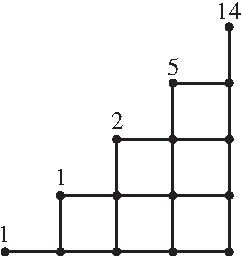
\includegraphics[width=0.33\linewidth]{images/CatalanPaths}
\caption{The lattice paths from \((0,0)\) to \((i,i)\) for \(i=0,1,2,3,4\).  The number of paths to the point \((i,i)\) is shown just above that point.\label{CatalanPaths}}
\end{figure}
\begin{enumerate}[font=\bfseries,label=(\alph*),ref=\alph*]
\item\label{task-56} \marginsymbol[-2.5em]{} \hypertarget{p-299}{}%
Explain why the number of lattice paths from \((0,0)\) to \((n,n)\) that go outside the triangle is the number of lattice paths from \((0,0)\) to \((n,n)\) that either touch or cross the line \(y=x+1\).%
\item\label{task-57} \marginsymbol[-2.5em]{} \hypertarget{p-301}{}%
Find a bijection between lattice paths from \((0,0)\) to \((n,n)\) that touch (or cross) the line \(y=x+1\) and lattice paths from \((-1,1)\) to \((n,n)\).%
~{\tiny (h)}\item\label{task-58} \marginsymbol[-2.5em]{} \hypertarget{p-304}{}%
Find a formula for the number of lattice paths from \((0,0)\) to \((n,n)\) that do not go above the line \(y=x\).  The number of such paths is called a \terminology{Catalan Number}\index{Catalan Number} and is usually denoted by \(C_n\).%
~{\tiny (h)}\end{enumerate}
\end{activity}
\begin{activity}[]\marginsymbol[-1em]{\pdftooltip{$\importantarrow$}{especially interesting}} \label{activity-52}
\hypertarget{p-307}{}%
Your formula for the Catalan Number can be expressed as a binomial coefficient divided by an integer. Whenever we have a formula that calls for division by an integer, an ideal combinatorial explanation of the formula is one that uses the quotient principle. The purpose of this problem is to find such an explanation using diagonal lattice paths.\footnote{The result we will derive is called the Chung-Feller Theorem\index{Chung-Feller Theorem}; this approach is based of a paper of Wen-jin Woan ``Uniform Partitions of Lattice Paths and Chung-Feller Generalizations,'' \textsl{American Mathematics Monthly} 58 June/July 2001, p556.\label{fn-3}} A diagonal lattice path that never goes below the \(y\)-coordinate of its first point is called a \terminology{Dyck Path}\index{Dyck path}. We will call a Dyck Path from \((0,0)\) to \((2n,0)\) a \terminology{Catalan Path}\index{Catalan Path} of length \(2n\). Thus the number of Catalan Paths of length \(2n\) is the Catalan Number \(C_n\).%
\begin{enumerate}[font=\bfseries,label=(\alph*),ref=\alph*]
\item\label{task-59} \marginsymbol[-2.5em]{} \hypertarget{p-308}{}%
If a Dyck Path has \(n\) steps (each an upstep or downstep), why do the first \(k\) steps form a Dyck Path for each nonnegative \(k\le n\)?%
\item\label{task-60} \marginsymbol[-2.5em]{} \hypertarget{p-310}{}%
Thought of as a curve in the plane, a diagonal lattice path can have many local maxima and minima, and can have several absolute maxima and minima, that is, several highest points and several lowest points. What is the \(y\)-coordinate of an absolute minimum point of a Dyck Path starting at \((0,0)\)?  Explain why a Dyck Path whose rightmost absolute minimum point is its last point is a Catalan Path.%
~{\tiny (h)}\item\label{task-61} \marginsymbol[-2.5em]{} \hypertarget{p-313}{}%
Let \(D\) be the set of all diagonal lattice paths from \((0,0)\) to \((2n,0)\).  (Thus these paths can go below the \(x\)-axis.) Suppose we partition \(D\) by letting \(B_i\) be the set of lattice paths in \(D\) that have \(i\) upsteps (perhaps mixed with some downsteps) following the last absolute minimum.  How many blocks does this partition have?  Give a succinct description of the block \(B_0\).%
~{\tiny (h)}\item\label{task-62} \marginsymbol[-2.5em]{} \hypertarget{p-316}{}%
How many upsteps are in a Catalan Path?%
\item\label{task-63} \marginsymbol[-2.5em]{\pdftooltip{$*$}{difficult}} \hypertarget{p-318}{}%
We are going to give a bijection between the set of Catalan Paths and the block \(B_i\) for each \(i\) between \(1\) and \(n\).  For now, suppose the value of \(i\), while unknown, is fixed.  We take a Catalan path and break it into three pieces.  The piece \(F\) (for ``front'') consists of all steps before the \(i\)th upstep in the Catalan path.  The piece \(U\) (for ``up'') consists of the \(i\)th upstep.  The piece \(B\) (for ``back'') is the portion of the path that follows the \(i\)th upstep.  Thus we can think of the path as \(FUB\).  Show that the function that takes \(FUB\) to \(BUF\) is a bijection from the set of Catalan Paths onto the block \(B_i\) of the partition.  (Notice that \(BUF\) can go below the \(x\) axis.)%
~{\tiny (h)}\item\label{task-64} \marginsymbol[-2.5em]{} \hypertarget{p-321}{}%
Explain how you have just given another proof of the formula for the Catalan Numbers.%
\end{enumerate}
\end{activity}
\typeout{************************************************}
\typeout{Subsection 1.3.2 The Binomial Theorem}
\typeout{************************************************}
\subsection[{The Binomial Theorem}]{The Binomial Theorem}\label{subsection-8}
\begin{activity}[]\marginsymbol[-1em]{\pdftooltip{$\circ$}{motivational material}} \label{Conjecturebinomthm}
\hypertarget{p-323}{}%
We know that \((x+y)^2 = x^2+2xy+y^2\). Multiply both sides by \((x+y)\) to get a formula for \((x+y)^3\) and repeat to get a formula for \((x+y)^4\). Do you see a pattern? If so, what is it? If not, repeat the process to get a formula for \((x+y)^5\) and look back at \hyperref[Pascaltriangle]{Figure~\ref{Pascaltriangle}} to see the pattern. Conjecture a formula for \((x+y)^n\).%
\end{activity}
\begin{activity}[]\marginsymbol[-1em]{\pdftooltip{$\bullet$}{essential}} \label{activity-54}
\hypertarget{p-328}{}%
When we apply the distributive law \(n\) times to \((x+y)^n\), we get a sum of terms of the form \(x^iy^{n-i}\) for various values of the integer \(i\). If it is clear to you that each term of the form \(x^iy^{n-i}\) that we get comes from choosing an \(x\) from \(i\) of the \((x+y)\) factors and a \(y\) from the remaining \(n-i\) of the factors and multiplying these choices together, then answer \hyperref[bin-thm-short]{part~a} of the problem and skip \hyperref[bin-thm-long]{part~b}. In either case, be sure to answer \hyperref[bin-thm-concl]{part~c}.%
\begin{enumerate}[font=\bfseries,label=(\alph*),ref=\alph*]
\item\label{bin-thm-short} \marginsymbol[-2.5em]{} \hypertarget{p-329}{}%
In how many ways can we choose an \(x\) from \(i\) terms and a \(y\) from \(n-i\) terms?%
\item\label{bin-thm-long} \marginsymbol[-2.5em]{} \hypertarget{p-331}{}%
We can take this step-by-step and consider a small case to get started.%
\begin{enumerate}[font=\bfseries,label=(\roman*),ref=\theenumi.\roman*]
\item\label{task-67} \marginsymbol[-2.5em]{} \hypertarget{p-332}{}%
Expand the product \((x_1 +y_1)(x_2 +y_2)(x_3+y_3)\).%
\item\label{task-68} \marginsymbol[-2.5em]{} \hypertarget{p-334}{}%
What do you get when you substitute \(x\) for each \(x_i\) and \(y\) for each \(y_i\)?%
\item\label{task-69} \marginsymbol[-2.5em]{} \hypertarget{p-336}{}%
Now imagine expanding%
\begin{equation*}
(x_1+y_1)(x_2+y_2)\cdots (x_n+y_n).
\end{equation*}
Once you apply the commutative law to the individual terms you get, you will have a sum of terms of the form%
\begin{equation*}
x_{k_1}x_{k_2}\cdots x_{k_i}\cdot y_{j_1}y_{j_2}\cdots
y_{j_{n-i}}.
\end{equation*}
What is the set \(\{k_1,k_2,\ldots, k_i\}\cup \{j_1,j_2,\ldots, j_{n-i}\}\)?%
\item\label{task-70} \marginsymbol[-2.5em]{} \hypertarget{p-338}{}%
In how many ways can you choose the set \(\{k_1,k_2,\ldots, k_i\}\)?%
\item\label{task-71} \marginsymbol[-2.5em]{} \hypertarget{p-340}{}%
Once you have chosen this set, how many choices do you have for \(\{j_1,j_2,\ldots, j_{n-i}\}\)?%
\item\label{task-72} \marginsymbol[-2.5em]{} \hypertarget{p-342}{}%
If you substitute \(x\) for each \(x_i\) and \(y\) for each \(y_i\), how many terms of the form \(x^iy^{n-i}\) will you have in the expanded product%
\begin{equation*}
(x_1+y_1)(x_2+y_2)\cdots (x_n+y_n)=(x+y)^n?
\end{equation*}
%
\item\label{task-73} \marginsymbol[-2.5em]{} \hypertarget{p-344}{}%
How many terms of the form \(x^{n-i}y^i\) will you have?%
\end{enumerate}
\item\label{bin-thm-concl} \marginsymbol[-2.5em]{} \hypertarget{p-346}{}%
Explain how you have just proved your conjecture from \hyperref[Conjecturebinomthm]{Problem~\ref{Conjecturebinomthm}}.  The theorem you have proved is called the \terminology{Binomial Theorem}.\index{Binomial Theorem}%
\end{enumerate}
\end{activity}
\begin{activity}[]\marginsymbol[-1em]{} \label{activity-55}
\hypertarget{p-348}{}%
What is \(\sum_{i=1}^{10} \binom{10}{i}3^i\)?%
~{\tiny (h)}\end{activity}
\begin{activity}[]\marginsymbol[-1em]{} \label{activity-56}
\hypertarget{p-351}{}%
What is \(\binom{n}{0}-\binom{n}{1}+\binom{n}{2}-\cdots \pm
\binom{n}{n}\) if \(n\) is an integer bigger than 0?%
~{\tiny (h)}\end{activity}
\begin{activity}[]\marginsymbol[-1em]{} \label{activity-57}
\hypertarget{p-354}{}%
Explain why%
\begin{equation*}
\sum_{i=0}^m\binom{m}{i}\binom{n}{k-i} = \binom{m+n}{k}.
\end{equation*}
Find two different explanations.%
~{\tiny (h)}~{\tiny (h)}\end{activity}
\begin{activity}[]\marginsymbol[-1em]{\pdftooltip{$\importantarrow$}{especially interesting}} \label{activity-58}
\hypertarget{p-359}{}%
From the symmetry of the binomial coefficients, it is not too hard to see that when \(n\) is an odd number, the number of subsets of \(\{1,2,\ldots,n\}\) of odd size equals the number of subsets of \(\{1,2,\ldots,n\}\) of even size. Is it true that when \(n\) is even the number of subsets of \(\{1,2,\ldots,n\}\) of even size equals the number of subsets of odd size? Why or why not?%
~{\tiny (h)}\end{activity}
\begin{activity}[]\marginsymbol[-1em]{\pdftooltip{$\importantarrow$}{especially interesting}} \label{activity-59}
\hypertarget{p-362}{}%
What is \(\sum_{i=0}^n i\binom{n}{i}\)? (Hint: think about how you might use calculus.)%
~{\tiny (h)}\end{activity}
\hypertarget{p-365}{}%
Notice how the proof you gave of the binomial theorem was a counting argument. It is interesting that an apparently algebraic theorem that tells us how to expand a power of a binomial is proved by an argument that amounts to counting the individual terms of the expansion. Part of the reason that combinatorial mathematics turns out to be so useful is that counting arguments often underlie important results of algebra. As the algebra becomes more sophisticated, so do the families of objects we have to count, but nonetheless we can develop a great deal of algebra on the basis of counting.%
\typeout{************************************************}
\typeout{Subsection 1.3.3 The pigeonhole principle}
\typeout{************************************************}
\subsection[{The pigeonhole principle}]{The pigeonhole principle}\label{subsection-9}
\begin{activity}[]\marginsymbol[-1em]{\pdftooltip{$\circ$}{motivational material}} \label{elevencoins}
\hypertarget{p-366}{}%
American coins are all marked with the year in which they were made. How many coins do you need to have in your hand to guarantee that on two (at least) of them, the date has the same last digit? (When we say ``to guarantee that on two (at least) of them,\textellipsis{}'' we mean that you can find two with the same last digit. You might be able to find three with that last digit, or you might be able to find one pair with the last digit 1 and one pair with the last digit 9, or any combination of equal last digits, as long as there is at least one pair with the same last digit.)%
\end{activity}
\hypertarget{p-368}{}%
There are many ways in which you might explain your answer to \hyperref[elevencoins]{Problem~\ref{elevencoins}}. For example, you can partition the coins according to the last digit of their date; that is, you put all the coins with a given last digit in a block together, and put no other coins in that block; repeating until all coins are in some block. Then you have a partition of your set of coins. If no two coins have the same last digit, then each block has exactly one coin. Since there are only ten digits, there are at most ten blocks and so by the sum principle there are at most ten coins. In fact with ten coins it is possible to have no two with the same last digit, but with 11 coins some block must have at least two coins in order for the sum of the sizes of at most ten blocks to be 11. This is one explanation of why we need 11 coins in \hyperref[elevencoins]{Problem~\ref{elevencoins}}. This kind of situation arises often in combinatorial situations, and so rather than always using the sum principle to explain our reasoning , we enunciate another principle which we can think of as yet another variant of the sum principle. The \terminology{pigeonhole principle}\index{pigeonhole principle} states that%
\begin{quote}\hypertarget{blockquote-7}{}
\hypertarget{p-369}{}%
If we partition a set with more than \(n\) elements into \(n\) parts, then at least one part has more than one element.%
\end{quote}
\hypertarget{p-370}{}%
The pigeonhole principle gets its name from the idea of a grid of little boxes that might be used, for example, to sort mail, or as mailboxes for a group of people in an office. The boxes in such grids are sometimes called pigeonholes in analogy with stacks of boxes used to house homing pigeons when homing pigeons were used to carry messages. People will sometimes state the principle in a more colorful way as ``if we put more than \(n\) pigeons into \(n\) pigeonholes, then some pigeonhole has more than one pigeon.''%
\begin{activity}[]\marginsymbol[-1em]{} \label{activity-61}
\hypertarget{p-371}{}%
Show that if we have a function from a set of size \(n\) to a set of size less than \(n\), then \(f\) is not one-to-one.%
~{\tiny (h)}\end{activity}
\begin{activity}[]\marginsymbol[-1em]{\pdftooltip{$\bullet$}{essential}} \label{activity-62}
\hypertarget{p-374}{}%
Show that if \(S\) and \(T\) are finite sets of the same size, then a function \(f\) from \(S\) to \(T\) is one-to-one if and only if it is onto.%
~{\tiny (h)}~{\tiny (h)}\end{activity}
\begin{activity}[]\marginsymbol[-1em]{\pdftooltip{\Large$\cdot$}{essential for this section or the next}} \label{activity-63}
\hypertarget{p-378}{}%
There is a \terminology{generalized pigeonhole principle}\index{pigeonhole principle!generalized} which says that if we partition a set with more than \(kn\) elements into \(n\) blocks, then at least one block has at least \(k+1\) elements. Prove the generalized pigeonhole principle.%
~{\tiny (h)}\end{activity}
\begin{activity}[]\marginsymbol[-1em]{} \label{activity-64}
\hypertarget{p-381}{}%
All the powers of five end in a five, and all the powers of two are even. Show that for for some integer \(n\), if you take the first \(n\) powers of a prime other than two or five, one must have ``01'' as the last two digits.%
~{\tiny (h)}\end{activity}
\begin{activity}[]\marginsymbol[-1em]{\pdftooltip{$\importantarrow$\ {\Large$\cdot$}}{especially interesting and essential for this or the next section}} \label{R_3_3_}
\hypertarget{p-384}{}%
Show that in a set of six people, there is a set of at least three people who all know each other, or a set of at least three people none of whom know each other. (We assume that if person 1 knows person 2, then person 2 knows person 1.)%
~{\tiny (h)}\end{activity}
\begin{activity}[]\marginsymbol[-1em]{\pdftooltip{\Large$\cdot$}{essential for this section or the next}} \label{notR_3_3_}
\hypertarget{p-387}{}%
Draw five circles labeled Al, Sue, Don, Pam, and Jo. Find a way to draw red and green lines between people so that every pair of people is joined by a line and there is neither a triangle consisting entirely of red lines or a triangle consisting of green lines. What does \hyperref[R_3_3_]{Problem~\ref{R_3_3_}} tell you about the possibility of doing this with six people's names? What does this problem say about the conclusion of \hyperref[R_3_3_]{Problem~\ref{R_3_3_}} holding when there are five people in our set rather than six?%
\end{activity}
\typeout{************************************************}
\typeout{Subsection 1.3.4 Ramsey Numbers}
\typeout{************************************************}
\subsection[{Ramsey Numbers}]{Ramsey Numbers}\label{Ramseysection}
\hypertarget{p-390}{}%
\hyperref[R_3_3_]{Problems~\ref{R_3_3_}--\ref{notR_3_3_}} together show that six is the smallest number \(R\) with the property that if we have \(R\) people in a room, then there is either a set of (at least) three mutual acquaintances or a set of (at least) three mutual strangers. Another way to say the same thing is to say that six is the smallest number so that no matter how we connect 6 points in the plane (no three on a line) with red and green lines, we can find either a red triangle or a green triangle. There is a name for this property. The \terminology{Ramsey Number} \(R(m,n)\) is the smallest number \(R\) so that if we have \(R\) people in a room, then there is a set of at least \(m\) mutual acquaintances or at least \(n\) mutual strangers. There is also a geometric description of Ramsey Numbers; it uses the idea of a \terminology{complete graph} on \(R\) vertices. A \terminology{complete graph}\index{graph!complete} on \(R\) vertices consists of \(R\) points in the plane together with line segments (or curves) connecting each two of the \(R\) vertices.\footnote{As you may have guessed, a complete graph is a special case of something called a graph.  The word graph will be defined in \hyperref[graphsection]{Subsection~\ref{graphsection}}.\label{fn-4}} The points are called \terminology{vertices}\index{vertex!of a complete graph}\index{vertex} and the line segments are called \terminology{edges}\index{edge!of a complete graph}\index{edge}. In \hyperref[completegraph]{Figure~\ref{completegraph}} we show three different ways to draw a complete graph on four vertices. We use \(K_n\) to stand for a complete graph on \(n\) vertices.%
\begin{figure}
\centering
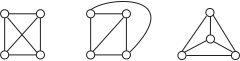
\includegraphics[width=0.5\linewidth]{images/threeK4s}
\caption{Three ways to draw a complete graph on four vertices\label{completegraph}}
\end{figure}
\hypertarget{p-391}{}%
Our geometric description of \(R(3,3)\) may be translated into the language of graph theory (which is the subject that includes complete graphs) by saying \(R(3,3)\) is the smallest number \(R\) so that if we color the edges of a \(K_R\) with two colors, then we can find in our picture a \(K_3\) all of whose edges have the same color.  The graph theory description of \(R(m,n)\) is that \(R(m,n)\) is the smallest number \(R\) so that if we color the edges of a \(K_R\) with red and green, then we can find in our picture either a \(K_m\) all of whose edges are red or a \(K_n\) all of whose edges are green. Because we could have said our colors in the opposite order, we may conclude that \(R(m,n) = R(n,m)\). In particular \(R(n,n)\) is the smallest number \(R\) such that if we color the edges of a \(K_R\) with two colors, then our picture contains a \(K_n\) all of whose edges have the same color.%
\begin{activity}[]\marginsymbol[-1em]{\pdftooltip{$\circ$}{motivational material}} \label{activity-67}
\hypertarget{p-392}{}%
Since \(R(3,3)=6\), an uneducated guess might be that \(R(4,4)=8\). Show that this is not the case.%
~{\tiny (h)}\end{activity}
\begin{activity}[]\marginsymbol[-1em]{\pdftooltip{\Large$\cdot$}{essential for this section or the next}} \label{not_R_4_3}
\hypertarget{p-395}{}%
Show that among ten people, there are either four mutual acquaintances or three mutual strangers. What does this say about \(R(4,3)\)?%
~{\tiny (h)}\end{activity}
\begin{activity}[]\marginsymbol[-1em]{\pdftooltip{\Large$\cdot$}{essential for this section or the next}} \label{OddNoPeople}
\hypertarget{p-398}{}%
Show that among an odd number of people there is at least one person who is an acquaintance of an even number of people and therefore also a stranger to an even number of people.%
~{\tiny (h)}\end{activity}
\begin{activity}[]\marginsymbol[-1em]{\pdftooltip{\Large$\cdot$}{essential for this section or the next}} \label{R_4_3_not8}
\hypertarget{p-401}{}%
Find a way to color the edges of a \(K_8\) with red and green so that there is no red \(K_4\) and no green \(K_3\).%
~{\tiny (h)}\end{activity}
\begin{activity}[]\marginsymbol[-1em]{\pdftooltip{$\importantarrow$\ {\Large$\cdot$}}{especially interesting and essential for this or the next section}} \label{activity-71}
\hypertarget{p-404}{}%
Find \(R(4,3)\).%
~{\tiny (h)}\end{activity}
\hypertarget{p-407}{}%
As of this writing, relatively few Ramsey Numbers are known. \(R(3,n)\) is known for \(n\lt 10\), \(R(4,4) = 18\), and \(R(5,4)=R(4,5)=25\).%
\typeout{************************************************}
\typeout{Supplementary Problems 1.4 Supplementary Chapter Problems}
\typeout{************************************************}
\section[{Supplementary Chapter Problems}]{Supplementary Chapter Problems}\label{sec_whatis-suppprobs}
\begin{exerciselist}
\item[1.]\marginsymbol[-1em]{\pdftooltip{$\importantarrow$}{especially interesting}} \hypertarget{compositiondefinition}{}\hypertarget{p-408}{}%
Remember that we can write \(n\) as a sum of \(n\) ones.  How many plus signs do we use?  In how many ways may we write \(n\) as a sum of a list of \(k\) positive numbers?  Such a list is called a \terminology{composition}\index{composition} of \(n\) into \(k\) parts.\index{composition!\(k\) parts}\index{composition!number of}%
\par\smallskip
\item[2.]\marginsymbol[-1em]{} \hypertarget{composition_numberof}{}\hypertarget{p-410}{}%
In \hyperlink{compositiondefinition}{Problem~1.4.1} we defined a composition of \(n\) into \(k\) parts.  What is the total number of compositions of \(n\) (into any number of parts). \index{compositions!number of}%
\par\smallskip
\item[3.]\marginsymbol[-1em]{\pdftooltip{\Large$\cdot$}{essential for this section or the next}} \hypertarget{GrayCode}{}\hypertarget{p-412}{}%
Write down a list of all 16 zero-one sequences of length four starting with 0000 in such a way that each entry differs from the previous one by changing just one digit.  This is called a Gray Code.\index{Gray Code} That is, a \terminology{Gray Code} for 0-1 sequences of length \(n\) is a list of the sequences so that each entry differs from the previous one in exactly one place.  Can you describe how to get a Gray Code for 0-1 sequences of length five from the one you found for sequences of length 4?  Can you describe how to prove that there is a Gray code for sequences of length \(n\)?%
\par\smallskip
\item[4.]\marginsymbol[-1em]{\pdftooltip{$\importantarrow$}{especially interesting}} \hypertarget{exercise-4}{}\hypertarget{p-414}{}%
Use the idea of a Gray code from \hyperlink{GrayCode}{Problem~1.4.3} to prove bijectively that the number of even-sized subsets of an \(n\)-element set equals the number of odd-sized subsets of an \(n\)-element set.%
\par\smallskip
\item[5.]\marginsymbol[-1em]{\pdftooltip{$\importantarrow$}{especially interesting}} \hypertarget{exercise-5}{}\hypertarget{p-416}{}%
A list of parentheses is said to be balanced if there are the same number of left parentheses as right, and as we count from left to right we always find at least as many left parentheses as right parentheses.  For example, (((()()))()) is balanced and ((()) and (()()))(() are not.  How many balanced lists of \(n\) left and \(n\) right parentheses are there?%
\par\smallskip
\item[6.]\marginsymbol[-1em]{\pdftooltip{$*$}{difficult}} \hypertarget{exercise-6}{}\hypertarget{p-418}{}%
Suppose we plan to put six distinct computers in a network as shown in \hyperref[hexagonalnetwork]{Figure~\ref{hexagonalnetwork}}.  The lines show which computers can communicate directly with which others.  Consider two ways of assigning computers to the nodes of the network different if there are two computers that communicate directly in one assignment and that don't communicate directly in the other.  In how many different ways can we assign computers to the network?%
\begin{figure}
\centering
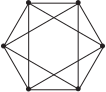
\includegraphics[width=0.33\linewidth]{images/HexagonalNetwork}
\caption{A computer network.\label{hexagonalnetwork}}
\end{figure}
\par\smallskip
\item[7.]\marginsymbol[-1em]{\pdftooltip{$\importantarrow$}{especially interesting}} \hypertarget{exercise-7}{}\hypertarget{p-420}{}%
In a circular ice cream dish we are going to put four distinct scoops of ice cream chosen from among twelve flavors.  Assuming we place four scoops of the same size as if they were at the corners of a square, and recognizing that moving the dish doesn't change the way in which we have put the ice cream into the dish, in how many ways may we choose the ice cream and put it into the dish?%
\par\smallskip
\item[8.]\marginsymbol[-1em]{\pdftooltip{$\importantarrow$}{especially interesting}} \hypertarget{exercise-8}{}\hypertarget{p-422}{}%
In as many ways as you can, show that \(\binom{n}{k}\binom{n-k}{m} =
\binom{n}{m}\binom{n-m}{k}\).%
\par\smallskip
\item[9.]\marginsymbol[-1em]{\pdftooltip{$\importantarrow$}{especially interesting}} \hypertarget{exercise-9}{}\hypertarget{p-426}{}%
A tennis club has \(4n\) members.  To specify a doubles match, we choose two teams of two people.  In how many ways may we arrange the members into doubles matches so that each player is in one doubles match?  In how many ways may we do it if we specify in addition who serves first on each team?%
\par\smallskip
\item[10.]\marginsymbol[-1em]{} \hypertarget{exercise-10}{}\hypertarget{p-428}{}%
A town has \(n\) streetlights running along the north side of main street.  The poles on which they are mounted need to be painted so that they do not rust.  In how many ways may they be painted with red, white, blue, and green if an even number of them are to be painted green?%
\par\smallskip
\item[11.]\marginsymbol[-1em]{\pdftooltip{$*$}{difficult}} \hypertarget{pingpongpaint}{}\hypertarget{p-430}{}%
We have \(n\) identical ping-pong balls.  In how many ways may we paint them red, white, blue, and green?%
\par\smallskip
\item[12.]\marginsymbol[-1em]{\pdftooltip{$*$}{difficult}} \hypertarget{exercise-12}{}\hypertarget{p-432}{}%
We have \(n\) identical ping-pong balls.  In how many ways may we paint them red, white, blue, and green if we use green paint on an even number of them?%
\par\smallskip
\end{exerciselist}
\typeout{************************************************}
\typeout{Chapter 2 Applications of Induction and Recursion in Combinatorics and Graph Theory}
\typeout{************************************************}
\chapter[{Applications of Induction and Recursion in Combinatorics and Graph Theory}]{Applications of Induction and Recursion in Combinatorics and Graph Theory}\label{InductionRecursion}
\typeout{************************************************}
\typeout{Section 2.1 Some Examples of Mathematical Induction}
\typeout{************************************************}
\section[{Some Examples of Mathematical Induction}]{Some Examples of Mathematical Induction}\label{sec_induction-examples}
\hypertarget{p-434}{}%
If you are unfamiliar with the Principle of Mathematical Induction, you should read \hyperref[Induction]{Appendix~\ref{Induction}} (a portion of which is repeated here).%
\typeout{************************************************}
\typeout{Subsection 2.1.1 Mathematical induction}
\typeout{************************************************}
\subsection[{Mathematical induction}]{Mathematical induction}\label{subsection-11}
\hypertarget{p-435}{}%
The \terminology{principle of mathematical induction}\index{mathematical induction!principle of}\index{principle of mathematical induction}\index{induction!mathematical, the principle of} states that%
\begin{quote}\hypertarget{blockquote-8}{}
\index{mathematical induction!principle of}\index{principle of mathematical induction}\index{induction!mathematical, the principle of}\hypertarget{p-436}{}%
In order to prove a statement about an integer \(n\), if we can \leavevmode%
\begin{enumerate}
\item\hypertarget{li-8}{}\hypertarget{p-437}{}%
Prove the statement when \(n=b\), for some fixed integer \(b\)%
\item\hypertarget{li-9}{}\hypertarget{p-438}{}%
Show that the truth of the statement for \(n=k-1\) implies the truth of the statement for \(n=k\) whenever \(k>b\),%
\end{enumerate}
 then we can conclude the statement is true for all integers \(n\ge
b\).%
\end{quote}
\hypertarget{p-439}{}%
As an example, let us give yet another proof that a set with \(n\) elements has \(2^n\) subsets. This proof uses essentially the same bijections we used in proving the Pascal Equation. The statement we wish to prove is the statement that ``A set of size \(n\) has \(2^n\) subsets.''%
\begin{quote}\hypertarget{blockquote-9}{}
\hypertarget{p-440}{}%
Our statement is true when \(n=0\), because a set of size 0 is the empty set and the empty set has \(1=2^0\) subsets. (This step of our proof is called a \terminology{base step}.) Now suppose that \(k>0\) and every set with \(k-1\) elements has \(2^{k-1}\) subsets.  Suppose \(S=\{a_1,a_2,\ldots a_k\}\) is a set with \(k\) elements. We partition the subsets of \(S\) into two blocks.  Block \(B_1\) consists of the subsets that do not contain \(a_n\) and block \(B_2\) consists of the subsets that do contain \(a_n\).  Each set in \(B_1\) is a subset of \(\{a_1,a_2,\ldots a_{k-1}\}\), and each subset of \(\{a_1,a_2, \ldots
a_{k-1}\}\) is in \(B_1\).  Thus \(B_1\) is the set of all subsets of \(\{a_1,a_2,\ldots a_{k-1}\}\).  Therefore by our assumption in the first sentence of this paragraph, the size of \(B_1\) is \(2^{k-1}\).  Consider the function from \(B_2\) to \(B_1\) which takes a subset of \(S\) including \(a_k\) and removes \(a_k\) from it.  This function is defined on \(B_2\), because every set in \(B_2\) contains \(a_k\).  This function is onto, because if \(T\) is a set in \(B_1\), then \(T\cup \{a_k\}\) is a set in \(B_2\) which the function sends to \(T\).  This function is one-to-one because if \(V\) and \(W\) are two different sets in \(B_2\), then removing \(a_k\) from them gives two different sets in \(B_1\).  Thus we have a bijection between \(B_1\) and \(B_2\), so \(B_1\) and \(B_2\) have the same size.  Therefore by the sum principle the size of \(B_1\cup B_2\) is \(2^{k-1} +2^{k-1}=2^k\).  Therefore \(S\) has \(2^k\) subsets.  This shows that if a set of size \(k-1\) has \(2^{k-1}\) subsets, then a set of size \(k\) has \(2^k\) subsets.  Therefore by the principle of mathematical induction, a set of size \(n\) has \(2^n\) subsets for every nonnegative integer \(n\).%
\end{quote}
\hypertarget{p-441}{}%
The first sentence of the last paragraph is called the \terminology{inductive hypothesis}. In an inductive proof we always make an inductive hypothesis as part of proving that the truth of our statement when \(n=k-1\) implies the truth of our statement when \(n=k\). The last paragraph itself is called the \terminology{inductive step} of our proof. In an inductive step we derive the statement for \(n=k\) from the statement for \(n=k-1\), thus proving that the truth of our statement when \(n=k-1\) implies the truth of our statement when \(n=k\). The last sentence in the last paragraph is called the \terminology{inductive conclusion}. All inductive proofs should have a base step, an inductive hypothesis, an inductive step, and an inductive conclusion.\index{inductive!hypothesis}\index{inductive!step}\index{inductive!conclusion}%
\par
\hypertarget{p-442}{}%
There are a couple details worth noticing. First, in this problem, our base step was the case \(n=0\), or in other words, we had \(b=0\). However, in other proofs, \(b\) could be any integer, positive, negative, or 0. Second, our proof that the truth of our statement for \(n=k-1\) implies the truth of our statement for \(n=k\) required that \(k\) be at least 1, so that there would be an element \(a_k\) we could take away in order to describe our bijection. However, condition (2) of the principle of mathematical induction only requires that we be able to prove the implication for \(k>0\), so we were allowed to assume \(k>0\).%
\typeout{************************************************}
\typeout{Subsubsection 2.1.1 Strong Mathematical Induction}
\typeout{************************************************}
\subsubsection[{Strong Mathematical Induction}]{Strong Mathematical Induction}\label{subsubsection-1}
\hypertarget{p-443}{}%
One way of looking at the principle of mathematical induction is that it tells us that if we know the ``first'' case of a theorem and we can derive each other case of the theorem from a smaller case, then the theorem is true in all cases. However the particular way in which we stated the theorem is rather restrictive in that it requires us to derive each case from the immediately preceding case. This restriction is not necessary, and removing it leads us to a more general statement of the principal of mathematical induction which people often call the \terminology{strong principle of mathematical induction}. It states:%
\begin{quote}\hypertarget{blockquote-10}{}
\index{strong principle of mathematical induction}\index{induction!mathematical, the strong principle of}\hypertarget{p-444}{}%
In order to prove a statement about an integer \(n\) if we can \leavevmode%
\begin{enumerate}
\item\hypertarget{li-10}{}\hypertarget{p-445}{}%
prove our statement when \(n=b\) and%
\item\hypertarget{li-11}{}\hypertarget{p-446}{}%
prove that the statements we get with \(n=b\), \(n=b+1\), \textellipsis{} \(n=k-1\) imply the statement with \(n=k\),%
\end{enumerate}
 then our statement is true for all integers \(n\ge b\).%
\end{quote}
\hypertarget{p-447}{}%
You will find some explicit examples of the use of the strong principle of mathematical induction in \hyperref[Induction]{Appendix~\ref{Induction}} and will find some uses for it in this chapter.%
\typeout{************************************************}
\typeout{Subsection 2.1.2 Binomial Coefficients and the Binomial Theorem}
\typeout{************************************************}
\subsection[{Binomial Coefficients and the Binomial Theorem}]{Binomial Coefficients and the Binomial Theorem}\label{subsection-12}
\begin{activity}[]\marginsymbol[-1em]{\pdftooltip{$\bullet$}{essential}} \label{activity-72}
\hypertarget{p-448}{}%
When we studied the Pascal Equation and subsets in \hyperref[what-is]{Chapter~\ref{what-is}}, it may have appeared that there is no connection between the Pascal relation \(\binom{n}{k} = \binom{n-1}{k-1} +\binom{n-1}{k}\) and the formula \(\binom{n}{k}=\frac{n!}{k!(n-k)!}\). Of course you probably realize you can prove the Pascal relation by substituting the values the formula gives you into the right-hand side of the equation and simplifying to give you the left hand side. In fact, from the Pascal Relation and the facts that \(\binom{n}{0}=1\) and \(\binom{n}{n}=1\), you can actually prove the formula for \(\binom{n}{k}\) by induction on \(n\). Do so.%
~{\tiny (h)}\end{activity}
\begin{activity}[]\marginsymbol[-1em]{\pdftooltip{$\importantarrow$}{especially interesting}} \label{activity-73}
\hypertarget{p-452}{}%
Use the fact that \((x+y)^n = (x+y)(x+y)^{n-1}\) to give an inductive proof of the binomial theorem.%
~{\tiny (h)}\end{activity}
\begin{activity}[]\marginsymbol[-1em]{} \label{activity-74}
\hypertarget{p-457}{}%
Suppose that \(f\) is a function defined on the nonnegative integers such that \(f(0)=3\) and \(f(n)=2f(n-1)\). Find a formula for \(f(n)\) and prove your formula is correct.%
\end{activity}
\begin{activity}[]\marginsymbol[-1em]{} \label{altproofnumberoffunctionsconjecture}
\hypertarget{p-459}{}%
Prove the conjecture in \hyperref[numberoffunctionsconjecture]{Part~\ref{countingfunctions2}.\ref{numberoffunctionsconjecture}} for an arbitrary positive integer \(m\) without appealing to the general product principle.%
~{\tiny (h)}\end{activity}
\typeout{************************************************}
\typeout{Subsection 2.1.3 Inductive definition}
\typeout{************************************************}
\subsection[{Inductive definition}]{Inductive definition}\label{subsection-13}
\hypertarget{p-461}{}%
You may have seen \(n!\)\index{factorial} described by the two equations \(0!=1\) and \(n!=n(n-1)!\) for \(n>0\). By the principle of mathematical induction we know that this pair of equations defines \(n!\) for all nonnegative numbers \(n\). For this reason we call such a definition an \terminology{inductive definition}\index{inductive definition}\index{definition!inductive}. An inductive definition is sometimes called a \terminology{recursive definition}\index{recursive definition}\index{definition!recursive}. Often we can get very easy proofs of useful facts by using inductive definitions.%
\begin{activity}[]\marginsymbol[-1em]{\pdftooltip{$\importantarrow$}{especially interesting}} \label{activity-76}
\hypertarget{p-462}{}%
An inductive definition of \(a^n\) for nonnegative \(n\) is given by \(a^0=1\) and \(a^n=aa^{n-1}\). (Notice the similarity to the inductive definition of \(n!\).) We remarked above that inductive definitions often give us easy proofs of useful facts. Here we apply this inductive definition to prove two useful facts about exponents that you have been using almost since you learned the meaning of exponents.%
\begin{enumerate}[font=\bfseries,label=(\alph*),ref=\alph*]
\item\label{task-75} \marginsymbol[-2.5em]{} \hypertarget{p-463}{}%
Use this definition to prove the rule of exponents \(a^{m+n}=a^ma^n\) for nonnegative \(m\) and \(n\).%
~{\tiny (h)}\item\label{task-76} \marginsymbol[-2.5em]{} \hypertarget{p-467}{}%
Use this definition to prove the rule of exponents \(a^{mn} =
(a^m)^n\).%
~{\tiny (h)}\end{enumerate}
\end{activity}
\begin{activity}[]\marginsymbol[-1em]{\pdftooltip{\tiny$+$}{summary}} \label{activity-77}
\hypertarget{p-471}{}%
Suppose that \(f\) is a function on the nonnegative integers such that \(f(0)=0\) and \(f(n) = n+f(n-1)\). Prove that \(f(n) = n(n+1)/2\). Notice that this gives a third proof that \(1+2+\cdots+n=n(n+1)/2\), because this sum satisfies the two conditions for \(f\). (The sum has no terms and is thus 0 when \(n=0\).)%
\end{activity}
\begin{activity}[]\marginsymbol[-1em]{\pdftooltip{$\importantarrow$}{especially interesting}} \label{activity-78}
\hypertarget{p-473}{}%
Give an inductive definition of the summation notation \(\sum_{i=1}^n a_i\). Use it and the distributive law \(b(a+c) = ba+bc\) to prove the distributive law%
\begin{equation*}
b\sum_{i=1}^n a_i = \sum_{i=1}^n ba_i.
\end{equation*}
%
\end{activity}
\typeout{************************************************}
\typeout{Subsection 2.1.4 Proving the general product principle (Optional)}
\typeout{************************************************}
\subsection[{Proving the general product principle (Optional)}]{Proving the general product principle (Optional)}\label{subsection-14}
\hypertarget{p-475}{}%
We stated the sum principle as%
\begin{quote}\hypertarget{blockquote-11}{}
\hypertarget{p-476}{}%
If we have a partition of a set \(S\), then the size of \(S\) is the sum of the sizes of the blocks of the partition.%
\end{quote}
\hypertarget{p-477}{}%
In fact, the simplest form of the sum principle says that the size of the sum of two disjoint (finite) sets is the sum of their sizes.%
\begin{activity}[]\marginsymbol[-1em]{} \label{activity-79}
\hypertarget{p-478}{}%
Prove the sum principle we stated for partitions of a set from the simplest form of the sum principle.%
~{\tiny (h)}\end{activity}
\hypertarget{p-482}{}%
We stated the simplest form of the product principle as%
\begin{quote}\hypertarget{blockquote-12}{}
\hypertarget{p-483}{}%
If we have a partition of a set \(S\) into \(m\) blocks, each of size \(n\), then \(S\) has size \(mn\).%
\end{quote}
\hypertarget{p-484}{}%
In \hyperref[generalproductprinciple]{Problem~\ref{generalproductprinciple}} we gave a more general form of the product principle which can be stated as \index{product principle!general}\index{general product principle}%
\begin{quote}\hypertarget{blockquote-13}{}
\hypertarget{p-485}{}%
Let \(S\) be a set of functions \(f\) from \([n]\) to some set \(X\).  Suppose that \leavevmode%
\begin{itemize}[label=\textbullet]
\item{}\hypertarget{p-486}{}%
there are \(k_1\) choices for \(f(1)\), and%
\item{}\hypertarget{p-487}{}%
suppose that for each choice of \(f(1)\), \(f(2)\), \textellipsis{} \(f(i-1)\), there are \(k_i\) choices for \(f(i)\).%
\end{itemize}
 Then the number of functions in the set \(S\) is \(k_1k_2\cdots k_n\).%
\end{quote}
\begin{activity}[]\marginsymbol[-1em]{\pdftooltip{\tiny$+$}{summary}} \label{generalproductprincipleproof}
\hypertarget{p-488}{}%
Prove the general form of the product principle from the simplest form of the product principle.%
~{\tiny (h)}\end{activity}
\typeout{************************************************}
\typeout{Subsection 2.1.5 Double Induction and Ramsey Numbers}
\typeout{************************************************}
\subsection[{Double Induction and Ramsey Numbers}]{Double Induction and Ramsey Numbers}\label{subsection-15}
\hypertarget{p-491}{}%
In \hyperref[Ramseysection]{Section~\ref{Ramseysection}} we gave two different descriptions of the Ramsey number \(R(m,n)\). However if you look carefully, you will see that we never showed that Ramsey numbers actually exist; we merely described what they were and showed that \(R(3,3)\) and \(R(3,4)\) exist by computing them directly. As long as we can show that there is some number \(R\) such that when there are \(R\) people together, there are either \(m\) mutual acquaintances or \(n\) mutual strangers, this shows that the Ramsey Number \(R(m,n)\) exists, because it is the smallest such \(R\). Mathematical induction allows us to show that one such \(R\) is \(\binom{m+n-2}{m-1}\). The question is, what should we induct on, \(m\) or \(n\)? In other words, do we use the fact that with \(\binom{m+n-3}{m-2}\) people in a room there are at least \(m-1\) mutual acquaintances or \(n\) mutual strangers, or do we use the fact that with at least \(\binom{m+n-3}{n-2}\) people in a room there are at least \(m\) mutual acquaintances or at least \(n-1\) mutual strangers? It turns out that we use both. Thus we want to be able to simultaneously induct on \(m\) and \(n\). One way to do that is to use yet another variation on the principle of mathematical induction, the \terminology{Principle of Double Mathematical Induction}\index{double induction}\index{induction!double}\index{mathematical induction!double}. This principle (which can be derived from one of our earlier ones) states that%
\begin{quote}\hypertarget{blockquote-14}{}
\index{double induction}\index{induction!double}\index{mathematical induction!double}\hypertarget{p-492}{}%
In order to prove a statement about  integers \(m\) and \(n\), if we can \leavevmode%
\begin{enumerate}
\item\hypertarget{li-18}{}\hypertarget{p-493}{}%
Prove the statement when \(m=a\) and \(n=b\), for  fixed integers \(a\) and \(b\)%
\item\hypertarget{li-19}{}\hypertarget{p-494}{}%
Prove the statement when \(m=a\) and \(n>b\) and when \(m>a\)  and \(n=b\) (for the same fixed integers \(a\) and \(b\)),%
\item\hypertarget{li-20}{}\hypertarget{p-495}{}%
Show that the truth of the statement for \(m=j\) and \(n=k-1\) (with \(j\ge a\) and \(k>b\)) and the truth of the statement for \(m=j-1\) and \(n=k\) (with \(j>a\) and \(k\ge b\)) imply the truth of the statement for \(m=j\) and \(n=k\),%
\end{enumerate}
 then we can conclude the statement is true for all pairs of integers \(m\ge
a\) and \(n\ge b\).%
\end{quote}
\hypertarget{p-496}{}%
There is a strong version of double induction, and it is actually easier to state. The principle of \terminology{strong double mathematical induction} \index{strong double induction} \index{double induction!strong} \index{induction!strong double} \index{mathematical induction!strong double} says the following.%
\begin{quote}\hypertarget{blockquote-15}{}
\hypertarget{p-497}{}%
In order to prove a statement about integers \(m\) and \(n\), if we can \leavevmode%
\begin{enumerate}
\item\hypertarget{li-21}{}Prove the statement when \(m=a\) and \(n=b\), for fixed integers \(a\) and \(b\).%
\item\hypertarget{li-22}{}Show that the truth of the statemetn for values of \(m\) and \(n\) with \(a+b\leq m+n \lt k\) imples the truth of the statment for \(m+n=k\),%
\end{enumerate}
 then we can conclude that the statement is true for all pairs of integers \(m\geq a\) and \(n\geq b\).%
\end{quote}
\begin{activity}[]\marginsymbol[-1em]{\pdftooltip{$\importantarrow$\ {\Large$\cdot$}}{especially interesting and essential for this or the next section}} \label{Ramseybound}
\hypertarget{p-498}{}%
Prove that \(R(m,n)\) exists by proving that if there are \(\binom{m+n-2}{m-1}\) people in a room, then there are either at least \(m\) mutual acquaintances or at least \(n\) mutual strangers.%
~{\tiny (h)}~{\tiny (h)}\end{activity}
\begin{activity}[]\marginsymbol[-1em]{\pdftooltip{\Large$\cdot$}{essential for this section or the next}} \label{Ramseyrecurrence}
\hypertarget{p-502}{}%
Prove that \(R(m,n)\le R(m-1,n) + R(m,n-1)\).%
~{\tiny (h)}~{\tiny (h)}\end{activity}
\begin{activity}[]\marginsymbol[-1em]{\pdftooltip{$\importantarrow$\ {\Large$\cdot$}}{especially interesting and essential for this or the next section}} \label{Ramseybound2}
\leavevmode%
\begin{enumerate}[font=\bfseries,label=(\alph*),ref=\alph*]
\item\label{task-77} \marginsymbol[-2.5em]{} \hypertarget{p-506}{}%
What does the equation in \hyperref[Ramseyrecurrence]{Problem~\ref{Ramseyrecurrence}} tell us about \(R(4,4)\)?%
\item\label{task-78} \marginsymbol[-2.5em]{\pdftooltip{$*$}{difficult}} \hypertarget{p-508}{}%
Consider 17 people arranged in a circle such that each person is acquainted with the first, second, fourth, and eighth person to the right and the first, second, fourth, and eighth person to the left.  can you find a set of four mutual acquaintances?  Can you find a set of four mutual strangers?%
~{\tiny (h)}\item\label{task-79} \marginsymbol[-2.5em]{} \hypertarget{p-511}{}%
What is \(R(4,4)\)?%
\end{enumerate}
\end{activity}
\begin{activity}[]\marginsymbol[-1em]{} \label{activity-84}
\hypertarget{p-512}{}%
(Optional) Prove the inequality of \hyperref[Ramseybound]{Problem~\ref{Ramseybound}} by induction on \(m+n\).%
\end{activity}
\begin{activity}[]\marginsymbol[-1em]{} \label{activity-85}
\hypertarget{p-515}{}%
Use Stirling's approximation (\hyperref[Stirling_sapproximation]{Problem~\ref{Stirling_sapproximation}}) to convert the upper bound for \(R(n,n)\) that you get from \hyperref[Ramseybound]{Problem~\ref{Ramseybound}} to a multiple of a power of an integer.%
\end{activity}
\typeout{************************************************}
\typeout{Subsection 2.1.6 A bit of asymptotic combinatorics}
\typeout{************************************************}
\subsection[{A bit of asymptotic combinatorics}]{A bit of asymptotic combinatorics}\label{subsection-16}
\hypertarget{p-517}{}%
\hyperref[Ramseybound2]{Problem~\ref{Ramseybound2}} gives us an upper bound on \(R(n,n)\). A very clever technique due to Paul Erdös, called the ``probabilistic method,'' will give a lower bound. Since both bounds are exponential in \(n\), they show that \(R(n,n)\) grows exponentially as \(n\) gets large. An analysis of what happens to a function of \(n\) as \(n\) gets large is usually called an \terminology{asymptotic analysis}.\index{asymptotic combinatorics} The \terminology{probabilistic method}\index{probabilistic method}\index{method!probabilistic}, at least in its simpler forms, can be expressed in terms of averages, so one does not need to know the language of probability in order to understand it. We will apply it to Ramsey numbers in the next problem. Combined with the result of \hyperref[Ramseybound2]{Problem~\ref{Ramseybound2}}, this problem will give us that \(\sqrt{2}^{\rangle n}\lt R(n,n)\lt 2^{2n-2}\), so that we know that the Ramsey number \(R(n,n)\) grows exponentially with~\(n\).%
\begin{activity}[]\marginsymbol[-1em]{\pdftooltip{$\importantarrow$}{especially interesting}} \label{activity-86}
\hypertarget{p-518}{}%
Suppose we have two numbers \(n\) and \(m\). We consider all possible ways to color the edges of the complete graph \(K_m\) with two colors, say red and blue. For each coloring, we look at each \(n\)-element subset \(N\) of the vertex set \(M\) of \(K_m\). Then \(N\) together with the edges of of \(K_m\) connecting vertices in \(N\) forms a complete graph on \(n\) vertices. This graph, which we denote by \(K_N\), has its edges colored by the original coloring of the edges of \(K_m\).%
\begin{enumerate}[font=\bfseries,label=(\alph*),ref=\alph*]
\item\label{task-80} \marginsymbol[-2.5em]{} \hypertarget{p-519}{}%
Why is it that if there is no subset \(N\subseteq M\) so that all the edges of \(K_N\) are colored the same color, then \(R(n,n)>m\)?%
~{\tiny (h)}\item\label{task-81} \marginsymbol[-2.5em]{} \hypertarget{p-522}{}%
To apply the probabilistic method, we are going to compute the average, over all colorings of \(K_m\), of the number of sets \(N\subseteq M\) with \(|N|=n\) such that \(K_N\) \emph{does} have all its edges the same color. Explain why it is that if the average is less than 1, then for some coloring there is no set \(N\) such that \(K_N\) has all its edges colored the same color.  Why does this mean that \(R(n,n)>m\)?%
~{\tiny (h)}\item\label{task-82} \marginsymbol[-2.5em]{} \hypertarget{p-525}{}%
We call a \(K_N\) \terminology{monochromatic}\index{monochromatic subgraph} for a coloring \(c\) of \(K_m\) if the color \(c(e)\) assigned to edge \(e\) is the same for every edge \(e\) of \(K_N\).  Let us define \({ mono}(c,N)\) to be 1 if \(N\) is monochromatic for \(c\) and to be 0 otherwise.  Find a formula for the average number of monochromatic \(K_N\)s over all colorings of \(K_m\) that involves a double sum first over all edge colorings \(c\) of \(K_m\) and then over all \(n\)-element subsets \(N\subseteq M\) of \({
mono}(c,N)\).%
~{\tiny (h)}\item\label{task-83} \marginsymbol[-2.5em]{} \hypertarget{p-528}{}%
Show that your formula for the average reduces to \(2\binom{m}{n}\cdot2^{-\binom{n}{2}}\)%
~{\tiny (h)}\item\label{task-84} \marginsymbol[-2.5em]{} \hypertarget{p-531}{}%
Explain why \(R(n,n)>m\) if \(\binom{m}{n}\le 2^{\binom{n}{2} -1}\).%
~{\tiny (h)}\item\label{task-85} \marginsymbol[-2.5em]{\pdftooltip{$*$}{difficult}} \hypertarget{p-534}{}%
Explain why \(R(n,n)>\root n \of {n!2^{\binom{n}{2}-1}}\).%
~{\tiny (h)}\item\label{task-86} \marginsymbol[-2.5em]{} \hypertarget{p-537}{}%
By using Stirling's formula, show that if \(n\) is large enough, then \(R(n,n) > \sqrt{2^n} = \sqrt{2}^{n}\).  (Here large enough means large enough for Stiirling's formula to be reasonable accurate.)%
\end{enumerate}
\end{activity}
\typeout{************************************************}
\typeout{Section 2.2 Recurrence Relations}
\typeout{************************************************}
\section[{Recurrence Relations}]{Recurrence Relations}\label{sec_induction-recurrence}
\begin{activity}[]\marginsymbol[-1em]{} \label{activity-87}
\hypertarget{p-539}{}%
How is the number of subsets of an \(n\)-element set related to the number of subsets of an \((n - 1)\)-element set? Prove that you are correct.%
~{\tiny (h)}\end{activity}
\begin{activity}[]\marginsymbol[-1em]{} \label{activity-88}
\hypertarget{p-542}{}%
Explain why it is that the number of bijections from an \(n\)-element set to an \(n\)-element set is equal to \(n\) times the number of bijections from an \((n-1)\)-element subset to an \((n-1)\)-element set. What does this have to do with \hyperref[permutationasbijection]{Problem~\ref{permutationasbijection}}?%
\end{activity}
\hypertarget{p-544}{}%
We can summarize these observations as follows. If \(s_n\) stands for the number of subsets of an \(n\)-element set, then%
\begin{equation}
s_n =2s_{n-1},\label{subsetequation}
\end{equation}
and if \(b_n\) stands for the number of bijections from an \(n\)-element set to an \(n\)-element set, then%
\begin{equation}
b_n =
nb_{n-1}.\label{bijectionequation}
\end{equation}
%
\par
\hypertarget{p-545}{}%
\hyperref[subsetequation]{Equations~(\ref{subsetequation})} and \hyperref[bijectionequation]{(\ref{bijectionequation})} are examples of \terminology{recurrence equations} or \terminology{recurrence relations}. A \terminology{recurrence relation}\index{relation!recurrence}\index{recurrence relation} or simply a \terminology{recurrence}\index{recurrence} is an equation that expresses the \(n\)th term of a sequence \(a_n\) in terms of values of \(a_i\) for \(i\lt n\). Thus \hyperref[subsetequation]{Equations~(\ref{subsetequation})} and \hyperref[bijectionequation]{(\ref{bijectionequation})} are examples of recurrences.%
\typeout{************************************************}
\typeout{Subsection 2.2.1 Examples of recurrence relations}
\typeout{************************************************}
\subsection[{Examples of recurrence relations}]{Examples of recurrence relations}\label{subsection-17}
\hypertarget{p-546}{}%
Other examples of recurrences are%
\begin{equation}
a_n = a_{n-1} +
7,\label{arithmeticexample}
\end{equation}
%
\begin{equation}
a_n =3a_{n-1} + 2^n,\label{geometricdriven}
\end{equation}
%
\begin{equation}
a_n = a_{n-1} + 3a_{n-2},\mbox{
and}\label{secondorderlinear}
\end{equation}
%
\begin{equation}
a_n= a_1a_{n-1} + a_2a_{n-2}+\cdots +
a_{n-1}a_1.\label{Catalan-recurrence}
\end{equation}
%
\par
\hypertarget{p-547}{}%
A \terminology{solution}\index{recurrence!solution to} to a recurrence relation is a sequence that satisfies the recurrence relation. Thus a solution to \hyperref[subsetequation]{Recurrence~(\ref{subsetequation})} is \(s_n =2^n\). Note that \(s_n=17\cdot2^n\) and \(s_n=-13\cdot2^n\) are also solutions to \hyperref[subsetequation]{Recurrence~(\ref{subsetequation})}. What this shows is that a recurrence can have infinitely many solutions. In a given problem, there is generally one solution that is of interest to us. For example, if we are interested in the number of subsets of a set, then the solution to \hyperref[subsetequation]{Recurrence~(\ref{subsetequation})} that we care about is \(s_n=2^n\). Notice this is the only solution we have mentioned that satisfies \(s_0=1\).%
\begin{activity}[]\marginsymbol[-1em]{} \label{activity-89}
\hypertarget{p-548}{}%
Show that there is only one solution to \hyperref[subsetequation]{Recurrence~(\ref{subsetequation})} that satisfies \(s_0=1\).%
\end{activity}
\begin{activity}[]\marginsymbol[-1em]{} \label{activity-90}
\hypertarget{p-550}{}%
A first-order recurrence relation is one which expresses \(a_n\) in terms of \(a_{n-1}\) and other functions of \(n\), but which does not include any of the terms \(a_i\) for \(i\lt n-1\) in the equation.%
\begin{enumerate}[font=\bfseries,label=(\alph*),ref=\alph*]
\item\label{task-87} \marginsymbol[-2.5em]{} \hypertarget{p-551}{}%
Which of the \hyperref[subsetequation]{recurrences~(\ref{subsetequation})} through \hyperref[Catalan-recurrence]{(\ref{Catalan-recurrence})} are first order recurrences?%
\item\label{task-88} \marginsymbol[-2.5em]{} \hypertarget{p-553}{}%
Show that there is one and only one sequence \(a_n\) that is defined for every nonnegative integer \(n\), satisfies a given first order recurrence, and satisfies \(a_0=a\) for some fixed constant \(a\).%
~{\tiny (h)}\end{enumerate}
\end{activity}
\begin{figure}
\centering
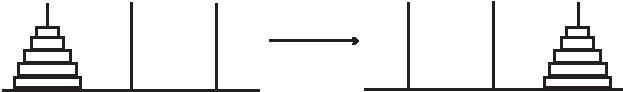
\includegraphics[width=0.85\linewidth]{images/Hanoi}
\caption{The Towers of Hanoi Puzzle\label{Hanoi}}
\end{figure}
\begin{activity}[]\marginsymbol[-1em]{\pdftooltip{$\importantarrow$}{especially interesting}} \label{HanoiProblem}
\hypertarget{p-556}{}%
The ``Towers of Hanoi'' puzzle has three rods rising from a rectangular base with \(n\) rings of different sizes stacked in decreasing order of size on one rod. A legal move consists of moving a ring from one rod to another so that it does not land on top of a smaller ring. If \(m_n\) is the number of moves required to move all the rings from the initial rod to another rod that you choose, give a recurrence for \(m_n\). (Hint: suppose you already knew the number of moves needed to solve the puzzle with \(n-1\) rings.)%
~{\tiny (h)}\end{activity}
\begin{activity}[]\marginsymbol[-1em]{\pdftooltip{$\importantarrow$}{especially interesting}} \label{circlesinplane}
\hypertarget{p-559}{}%
We draw \(n\) mutually intersecting circles in the plane so that each one crosses each other one exactly twice and no three intersect in the same point. (As examples, think of Venn diagrams with two or three mutually intersecting sets.) Find a recurrence for the number \(r_n\) of regions into which the plane is divided by \(n\) circles. (One circle divides the plane into two regions, the inside and the outside.) Find the number of regions with \(n\) circles. For what values of \(n\) can you draw a Venn diagram showing all the possible intersections of \(n\) sets using circles to represent each of the sets?%
~{\tiny (h)}~{\tiny (h)}\end{activity}
\typeout{************************************************}
\typeout{Subsection 2.2.2 Arithmetic Series (optional)}
\typeout{************************************************}
\subsection[{Arithmetic Series (optional)}]{Arithmetic Series (optional)}\label{subsection-18}
\begin{activity}[]\marginsymbol[-1em]{} \label{childsaving}
\hypertarget{p-564}{}%
A child puts away two dollars from her allowance each week. If she starts with twenty dollars, give a recurrence for the amount \(a_n\) of money she has after \(n\) weeks and find out how much money she has at the end of \(n\) weeks.%
\end{activity}
\begin{activity}[]\marginsymbol[-1em]{} \label{arithmeticprogression}
\hypertarget{p-566}{}%
A sequence that satisfies a recurrence of the form \(a_n=a_{n-1} +c\) is called an \terminology{arithmetic progression}\index{arithmetic progression}\index{progression!arithmetic}. Find a formula in terms of the initial value \(a_0\) and the common difference \(c\) for the term \(a_n\) in an arithmetic progression and prove you are right.%
\end{activity}
\begin{activity}[]\marginsymbol[-1em]{} \label{activity-95}
\hypertarget{p-568}{}%
A person who is earning \textdollar{}50,000 per year gets a raise of \textdollar{}3000 a year for \(n\) years in a row. Find a recurrence for the amount \(a_n\) of money the person earns over \(n+1\) years. What is the total amount of money that the person earns over a period of \(n+1\) years? (In \(n+1\) years, there are \(n\) raises.)%
\end{activity}
\begin{activity}[]\marginsymbol[-1em]{} \label{activity-96}
\hypertarget{p-570}{}%
An \terminology{arithmetic series}\index{series!arithmetic}\index{arithmetic series} is a sequence \(s_n\) equal to the sum of the terms \(a_0\) through \(a_n\) of of an arithmetic progression. Find a recurrence for the sum \(s_n\) of an arithmetic progression with initial value \(a_0\) and common difference \(c\) (using the language of \hyperref[arithmeticprogression]{Problem~\ref{arithmeticprogression}}). Find a formula for general term \(s_n\) of an arithmetic series.%
\end{activity}
\typeout{************************************************}
\typeout{Subsection 2.2.3 First order linear recurrences}
\typeout{************************************************}
\subsection[{First order linear recurrences}]{First order linear recurrences}\label{subsection-19}
\hypertarget{p-572}{}%
Recurrences such as those in \hyperref[subsetequation]{Equations~(\ref{subsetequation})} through \hyperref[secondorderlinear]{(\ref{secondorderlinear})} are called \terminology{linear recurrences}, as are the recurrences of \hyperref[HanoiProblem]{Problems~\ref{HanoiProblem}} and \hyperref[circlesinplane]{Problem~\ref{circlesinplane}}. A \terminology{linear recurrence}\index{recurrence!linear}\index{linear recurrence} is one in which \(a_n\) is expressed as a sum of functions of \(n\) times values of (some of the terms) \(a_i\) for \(i\lt n\) plus (perhaps) another function (called the \terminology{driving function}\index{driving function}\index{function!driving}) of \(n\). A linear equation is called \terminology{homogeneous}\index{homogeneous linear recurrence}\index{linear recurrence!homogeneous}\index{recurrence!linear homogeneous} if the driving function is zero (or, in other words, there is no driving function). It is called a \terminology{constant coefficient linear recurrence}\index{linear recurrence!constant coefficient}\index{constant coefficient linear recurrence} if the functions that are multiplied by the \(a_i\) terms are all constants (but the driving function need not be constant).%
\begin{activity}[]\marginsymbol[-1em]{} \label{classifyrecurrences}
\hypertarget{p-573}{}%
Classify the recurrences in \hyperref[subsetequation]{Equations~(\ref{subsetequation})} through \hyperref[secondorderlinear]{(\ref{secondorderlinear})} and \hyperref[HanoiProblem]{Problems~\ref{HanoiProblem}} and \hyperref[circlesinplane]{Problem~\ref{circlesinplane}} according to whether or not they are constant coefficient, and whether or not they are homogeneous.%
\end{activity}
\begin{activity}[]\marginsymbol[-1em]{\pdftooltip{$\bullet$}{essential}} \label{firstordlinconst}
\hypertarget{p-575}{}%
As you can see from \hyperref[classifyrecurrences]{Problem~\ref{classifyrecurrences}} some interesting sequences satisfy first order linear recurrences, including many that have constant coefficients, have constant driving term, or are homogeneous. Find a formula in terms of \(b\), \(d\), \(a_0\) and \(n\) for the general term \(a_n\) of a sequence that satisfies a constant coefficient first order linear recurrence \(a_n = ba_{n-1} + d\) and prove you are correct. If your formula involves a summation, try to replace the summation by a more compact expression.%
~{\tiny (h)}\end{activity}
\typeout{************************************************}
\typeout{Subsection 2.2.4 Geometric Series}
\typeout{************************************************}
\subsection[{Geometric Series}]{Geometric Series}\label{subsection-20}
\hypertarget{p-582}{}%
A sequence that satisfies a recurrence of the form \(a_n=ba_{n-1}\) is called a \terminology{geometric progression}\index{geometric progression}\index{progression!geometric}. Thus the sequence satisfying \hyperref[subsetequation]{Equation~(\ref{subsetequation})}, the recurrence for the number of subsets of an \(n\)-element set, is an example of a geometric progression. From your solution to \hyperref[firstordlinconst]{Problem~\ref{firstordlinconst}}, a geometric progression has the form \(a_n=a_0b^n\). In your solution to \hyperref[firstordlinconst]{Problem~\ref{firstordlinconst}} you may have had to deal with the sum of a geometric progression in just slightly different notation, namely \(\sum_{i=0}^{n-1}db^i\). A sum of this form is called a \terminology{(finite) geometric series}.\index{geometric series}\index{series!geometric}%
\begin{activity}[]\marginsymbol[-1em]{} \label{sumgeometricseries}
\hypertarget{p-583}{}%
Do this problem only if your final answer (so far) to \hyperref[firstordlinconst]{Problem~\ref{firstordlinconst}} contained the sum \(\sum_{i=0}^{n-1}db^i\).%
\begin{enumerate}[font=\bfseries,label=(\alph*),ref=\alph*]
\item\label{task-89} \marginsymbol[-2.5em]{} \hypertarget{p-584}{}%
Expand \((1-x)(1+x)\).  Expand \((1-x)(1+x+x^2)\). Expand \((1-x)(1+x+x^2+x^3)\).%
\item\label{task-90} \marginsymbol[-2.5em]{} \hypertarget{p-586}{}%
What do you expect \((1-b)\sum_{i=0}^{n-1} db^i\) to be?  What formula for \(\sum_{i=0}^{n-1}db^i\) does this give you?  Prove that you are correct.%
\end{enumerate}
\end{activity}
\hypertarget{p-589}{}%
In \hyperref[firstordlinconst]{Problem~\ref{firstordlinconst}} and \hyperref[sumgeometricseries]{perhaps~\ref{sumgeometricseries}} you proved an important theorem.%
\begin{theorem}[{}]\label{theorem-2}
\hypertarget{p-590}{}%
If \(b\not=1\) and \(a_n=ba_{n-1} +d\), then \(\displaystyle a_n =
a_0b^n + d\frac{1-b^n}{1-b}\). If \(b=1\), then, \(\displaystyle a_n =
a_0 +nd\)%
\end{theorem}
\begin{corollary}[{}]\label{corollary-1}
\hypertarget{p-591}{}%
If \(b\not=1\), then \(\displaystyle \sum_{i=0}^{n-1}b^i =
\frac{1-b^n}{1-b}\). If \(b=1\), \(\displaystyle \sum_{i=0}^{n-1}b^i =n\).%
\end{corollary}
\typeout{************************************************}
\typeout{Section 2.3 Graphs and Trees}
\typeout{************************************************}
\section[{Graphs and Trees}]{Graphs and Trees}\label{sec_induction-graphstrees}
\typeout{************************************************}
\typeout{Subsection 2.3.1 Undirected graphs}
\typeout{************************************************}
\subsection[{Undirected graphs}]{Undirected graphs}\label{graphsection}
\hypertarget{p-592}{}%
In \hyperref[Ramseysection]{Section~\ref{Ramseysection}} we introduced the idea of a directed graph. Graphs consist of vertices and edges. We describe vertices and edges in much the same way as we describe points and lines in geometry: we don't really say what vertices and edges are, but we say what they do. We just don't have a complicated axiom system the way we do in geometry. A \terminology{graph}\index{graph} consists of a set \(V\) called a vertex set and a set \(E\) called an edge set. Each member of \(V\) is called a \terminology{vertex}\index{vertex} and each member of \(E\) is called an \terminology{edge}.\index{edge} Associated with each edge are two (not necessarily different) vertices called its endpoints. We draw pictures of graphs by drawing points to represent the vertices and line segments (curved if we choose) whose endpoints are at vertices to represent the edges. In \hyperref[Threegraphs]{Figure~\ref{Threegraphs}} we show three pictures of graphs.%
\begin{figure}
\centering
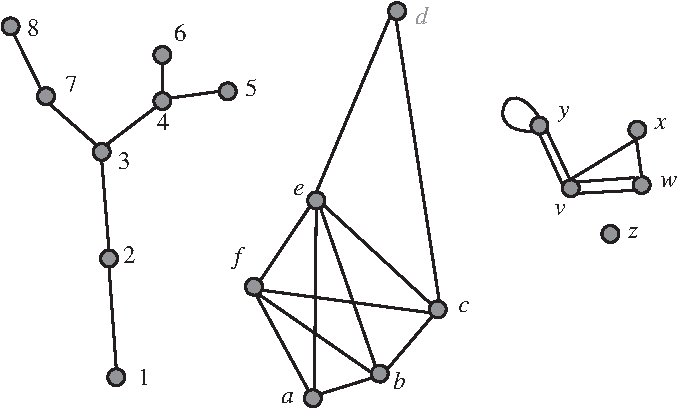
\includegraphics[width=0.95\linewidth]{images/threegraphs}
\caption{Three different graphs\label{Threegraphs}}
\end{figure}
\hypertarget{p-593}{}%
Each gray circle in the figure represents a vertex; each line segment represents an edge. You will note that we labelled the vertices; these labels are names we chose to give the vertices. We can choose names or not as we please. The third graph also shows that it is possible to have an edge that connects a vertex (like the one labelled \(y\)) to itself or it is possible to have two or more edges (like those between vertices \(v\) and \(y\)) between two vertices. The \terminology{degree}\index{vertex!degree of}\index{degree of a vertex} of a vertex is the number of times it appears as the endpoint of edges; thus the degree of \(y\) in the third graph in the figure is four.%
\begin{activity}[]\marginsymbol[-1em]{\pdftooltip{$\circ$}{motivational material}} \label{activity-100}
\hypertarget{p-594}{}%
In the graph on the left in \hyperref[Threegraphs]{Figure~\ref{Threegraphs}}, what is the degree of each vertex?%
\end{activity}
\begin{activity}[]\marginsymbol[-1em]{\pdftooltip{$\circ$}{motivational material}} \label{activity-101}
\hypertarget{p-596}{}%
For each graph in \hyperref[Threegraphs]{Figure~\ref{Threegraphs}} is the number of vertices of odd degree even or odd?%
\end{activity}
\begin{activity}[]\marginsymbol[-1em]{\pdftooltip{$\importantarrow$\ {\Large$\cdot$}}{especially interesting and essential for this or the next section}} \label{activity-102}
\hypertarget{p-598}{}%
The sum of the degrees of the vertices of a (finite) graph is related in a natural way to the number of edges.%
\begin{enumerate}[font=\bfseries,label=(\alph*),ref=\alph*]
\item\label{task-91} \marginsymbol[-2.5em]{} \hypertarget{p-599}{}%
What is the relationship?%
~{\tiny (h)}\item\label{task-92} \marginsymbol[-2.5em]{} \hypertarget{p-602}{}%
Find a proof that what you say is correct that uses induction on the number of edges.  Hint:  To make your inductive step, think about what happens to a graph if you delete an edge.%
~{\tiny (h)}\item\label{task-93} \marginsymbol[-2.5em]{} \hypertarget{p-605}{}%
Find a proof that what you say is correct that uses induction on the number of vertices.%
\item\label{task-94} \marginsymbol[-2.5em]{} \hypertarget{p-607}{}%
Find a proof that what you say is correct that does not use induction.%
~{\tiny (h)}\end{enumerate}
\end{activity}
\begin{activity}[]\marginsymbol[-1em]{\pdftooltip{\Large$\cdot$}{essential for this section or the next}} \label{activity-103}
\hypertarget{p-610}{}%
What can you say about the number of vertices of odd degree in a graph?%
~{\tiny (h)}\end{activity}
\typeout{************************************************}
\typeout{Subsection 2.3.2 Walks and paths in graphs}
\typeout{************************************************}
\subsection[{Walks and paths in graphs}]{Walks and paths in graphs}\label{subsection-22}
\hypertarget{p-613}{}%
A \terminology{walk}\index{walk} in a graph is an alternating sequence \(v_0e_1v_1\ldots
e_iv_i\) of vertices and edges such that edge \(e_i\) connects vertices \(v_{i-1}\) and \(v_i\). A graph is called connected if, for any pair of vertices, there is a walk starting at one and ending at the other.%
\begin{activity}[]\marginsymbol[-1em]{} \label{connectedanddisconnected}
\hypertarget{p-614}{}%
Which of the graphs in \hyperref[Threegraphs]{Figure~\ref{Threegraphs}} is connected?%
\end{activity}
\begin{activity}[]\marginsymbol[-1em]{\pdftooltip{$\circ$}{motivational material}} \label{activity-105}
\hypertarget{p-616}{}%
A \terminology{path}\index{path!in graph} in a graph is a walk with no repeated vertices.  Find the longest path you can in the third graph of \hyperref[Threegraphs]{Figure~\ref{Threegraphs}}.%
\end{activity}
\begin{activity}[]\marginsymbol[-1em]{\pdftooltip{$\circ$}{motivational material}} \label{activity-106}
\hypertarget{p-618}{}%
A \terminology{cycle}\index{cycle (in a graph)} in a graph is a walk whose first and last vertex are equal but which has no other repeated vertices.  Which graphs in \hyperref[Threegraphs]{Figure~\ref{Threegraphs}} have cycles?  What is the largest number of edges in a cycle in the second graph in \hyperref[Threegraphs]{Figure~\ref{Threegraphs}}?  What is the smallest number of edges in a cycle in the third graph in \hyperref[Threegraphs]{Figure~\ref{Threegraphs}}?%
\end{activity}
\begin{activity}[]\marginsymbol[-1em]{\pdftooltip{$\circ$}{motivational material}} \label{activity-107}
\hypertarget{p-620}{}%
A connected graph with no cycles is called a \terminology{tree}\index{tree}.  Which graphs, if any, in \hyperref[Threegraphs]{Figure~\ref{Threegraphs}} are trees?%
\end{activity}
\typeout{************************************************}
\typeout{Subsection 2.3.3 Counting vertices, edges, and paths in trees}
\typeout{************************************************}
\subsection[{Counting vertices, edges, and paths in trees}]{Counting vertices, edges, and paths in trees}\label{subsection-23}
\begin{activity}[]\marginsymbol[-1em]{\pdftooltip{$\importantarrow$\ {\Large$\cdot$}}{especially interesting and essential for this or the next section}} \label{Noverticesandedgesoftree}
\hypertarget{p-622}{}%
Draw some trees and on the basis of your examples, make a conjecture about the relationship between the number of vertices and edges in a tree. Prove your conjecture. (Hint: what happens if you choose an edge and delete it, but not its endpoints?)%
~{\tiny (h)}\end{activity}
\begin{activity}[]\marginsymbol[-1em]{\pdftooltip{\Large$\cdot$}{essential for this section or the next}} \label{activity-109}
\hypertarget{p-625}{}%
What is the minimum number of vertices of degree one in a finite tree? What is it if the number of vertices is bigger than one? Prove that you are correct.%
~{\tiny (h)}\end{activity}
\begin{activity}[]\marginsymbol[-1em]{\pdftooltip{$\importantarrow$\ {\Large$\cdot$}}{especially interesting and essential for this or the next section}} \label{activity-110}
\hypertarget{p-628}{}%
In a tree, given two vertices, how many paths can you find between them? Prove that you are correct.%
\end{activity}
\begin{activity}[]\marginsymbol[-1em]{\pdftooltip{$\importantarrow$\ $*$}{especially interesting and difficult}} \label{Prufer}
\hypertarget{p-630}{}%
How many trees are there on the vertex set \(\{1,2\}\)? On the vertex set \(\{1,2,3\}\)? When we label the vertices of our tree, we consider the tree which has edges between vertices 1 and 2 and between vertices 2 and 3 different from the tree that has edges between vertices 1 and 3 and between 2 and 3. See \hyperref[differenttrees]{Figure~\ref{differenttrees}}.%
\begin{figure}
\centering
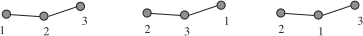
\includegraphics[width=0.8\linewidth]{images/threetrees}
\caption{The three labelled trees on three vertices\label{differenttrees}}
\end{figure}
\hypertarget{p-631}{}%
How many (labelled) trees are there on four vertices? You don't have a lot of data to guess from, but try to guess a formula for the number of labelled trees with vertex set \(\{1,2,\cdots,n\}\).%
~{\tiny (h)}\end{activity}
\hypertarget{p-634}{}%
We are now going to introduce a method to prove the formula you guessed. Given a tree with two or more vertices, labelled with positive integers, we define a sequence \(b_1,b_2,\ldots\) of integers inductively as follows: If the tree has two vertices, the sequence consists of one entry, namely the label of the vertex with the larger label. Otherwise, let \(a_1\) be the lowest numbered vertex of degree 1 in the tree. Let \(b_1\) be the label of the unique vertex in the tree adjacent to \(a_1\) and write down \(b_1\). For example, in the first graph in \hyperref[Threegraphs]{Figure~\ref{Threegraphs}}, \(a_1\) is 1 and \(b_1\) is 2. Given \(a_1\) through \(a_{i-1}\), let \(a_i\) be the lowest numbered vertex of degree 1 in the tree you get by deleting \(a_1\) through \(a_{i-1}\)and let \(b_i\) be the unique vertex in this new tree adjacent to \(a_i\). For example, in the first graph in \hyperref[Threegraphs]{Figure~\ref{Threegraphs}}, \(a_2=2\) and \(b_2=3\). Then \(a_3=5\) and \(b_3=4\). We use \(b\) to stand for the sequence of \(b_i\)s we get in this way. In the tree (the first graph) in \hyperref[Threegraphs]{Figure~\ref{Threegraphs}}, the sequence \(b\) is 2344378. (If you are unfamiliar with inductive (recursive) definition, you might want to write down some other labelled trees on eight vertices and construct the sequence of \(b_i\)s.)%
\begin{activity}[]\marginsymbol[-1em]{} \label{prufer-props}
\leavevmode%
\begin{enumerate}[font=\bfseries,label=(\alph*),ref=\alph*]
\item\label{task-95} \marginsymbol[-2.5em]{} \hypertarget{p-635}{}%
How long will the sequence of \(b_i\)s be if it is computed from a tree with \(n\) vertices (labelled with 1 through \(n\))?%
\item\label{task-96} \marginsymbol[-2.5em]{} \hypertarget{p-636}{}%
What can you say about the last member of the sequence of \(b_i\)s?%
~{\tiny (h)}\item\label{task-97} \marginsymbol[-2.5em]{} \hypertarget{p-638}{}%
Can you tell from the sequence of \(b_i\)s what \(a_1\)is?%
~{\tiny (h)}\item\label{task-98} \marginsymbol[-2.5em]{} \hypertarget{p-640}{}%
Find a bijection between labelled trees and something you can ``count'' that will tell you how many labelled trees there are on \(n\) labelled vertices.%
~{\tiny (h)}\end{enumerate}
\end{activity}
\hypertarget{p-642}{}%
The sequence \(b_1,b_2,\ldots, b_{n-2}\) in \hyperref[Prufer]{Problem~\ref{Prufer}} is called a \terminology{Prüfer coding} or \terminology{Prüfer code} for the tree. There is a good bit of interesting information encoded into the Prüfer code for a tree.%
\begin{activity}[]\marginsymbol[-1em]{} \label{activity-113}
\hypertarget{p-643}{}%
What can you say about the vertices of degree one from the Prüfer code for a tree labeled with the integers from 1 to \(b\)?%
~{\tiny (h)}\end{activity}
\begin{activity}[]\marginsymbol[-1em]{} \label{activity-114}
\hypertarget{p-645}{}%
What can you say about the Prüfer code for a tree with exactly two vertices of degree 1? (and perhaps some vertices with other degrees as well)? Does this characterize such trees?%
\end{activity}
\begin{activity}[]\marginsymbol[-1em]{\pdftooltip{$\importantarrow$}{especially interesting}} \label{activity-115}
\hypertarget{p-647}{}%
What can you determine about the degree of the vertex labelled \(i\) from the Prüfer code of the tree?%
~{\tiny (h)}\end{activity}
\begin{activity}[]\marginsymbol[-1em]{\pdftooltip{$\importantarrow$}{especially interesting}} \label{activity-116}
\hypertarget{p-650}{}%
What is the number of (labelled) trees on \(n\) vertices with three vertices of degree 1? (Assume they are labelled with the integers 1 through \(n\).) This problem will appear again in the next chapter after some material that will make it easier.%
~{\tiny (h)}\end{activity}
\typeout{************************************************}
\typeout{Subsection 2.3.4 Spanning trees}
\typeout{************************************************}
\subsection[{Spanning trees}]{Spanning trees}\label{subsection-24}
\hypertarget{p-653}{}%
Many of the applications of trees arise from trying to find an efficient way to connect all the vertices of a graph. For example, in a telephone network, at any given time we have a certain number of wires (or microwave channels, or cellular channels) available for use. These wires or channels go from a specific place to a specific place. Thus the wires or channels may be thought of as edges of a graph and the places the wires connect may be thought of as vertices of that graph. A tree whose edges are some of the edges of a graph \(G\) and whose vertices are all of the vertices of the graph \(G\) is called a \terminology{spanning tree}\index{spanning tree}\index{tree!spanning} of \(G\). A spanning tree for a telephone network will give us a way to route calls between any two vertices in the network. In \hyperref[spanningtrees]{Figure~\ref{spanningtrees}} we show a graph and all its spanning trees.%
\begin{figure}
\centering
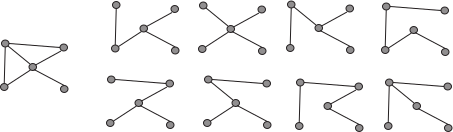
\includegraphics[width=0.95\linewidth]{images/spanningtrees}
\caption{A graph and all its spanning trees.\label{spanningtrees}}
\end{figure}
\begin{activity}[]\marginsymbol[-1em]{} \label{activity-117}
\hypertarget{p-654}{}%
Show that every connected graph has a spanning tree. It is possible to find a proof that starts with the graph and works ``down'' towards the spanning tree and to find a proof that starts with just the vertices and works ``up'' towards the spanning tree. Can you find both kinds of proof?%
\end{activity}
\typeout{************************************************}
\typeout{Subsection 2.3.5 Minimum cost spanning trees}
\typeout{************************************************}
\subsection[{Minimum cost spanning trees}]{Minimum cost spanning trees}\label{subsection-25}
\hypertarget{p-659}{}%
Our motivation for talking about spanning trees was the idea of finding a minimum number of edges we need to connect all the edges of a communication network together. In many cases edges of a communication network come with costs associated with them. For example, one cell-phone operator charges another one when a customer of the first uses an antenna of the other. Suppose a company has offices in a number of cities and wants to put together a communication network connecting its various locations with high-speed computer communications, but to do so at minimum cost. Then it wants to take a graph whose vertices are the cities in which it has offices and whose edges represent possible communications lines between the cities. Of course there will not necessarily be lines between each pair of cities, and the company will not want to pay for a line connecting city \(i\) and city \(j\) if it can already connect them indirectly by using other lines it has chosen. Thus it will want to choose a spanning tree of minimum cost among all spanning trees of the communications graph. For reasons of this application, if we have a graph with numbers assigned to its edges, the sum of the numbers on the edges of a spanning tree of \(G\) will be called the \terminology{cost}\index{spanning tree!cost of}\index{tree!spanning!cost of}\index{cost of a spanning tree} of the spanning tree.%
\begin{activity}[]\marginsymbol[-1em]{\pdftooltip{$\importantarrow$}{especially interesting}} \label{mincostspantree}
\hypertarget{p-660}{}%
Describe a method (or better, two methods different in at least one aspect) for finding a spanning tree of minimum cost in a graph whose edges are labelled with costs, the cost on an edge being the cost for including that edge in a spanning tree. Prove that your method(s) work.\index{minimum cost spanning tree}\index{spanning tree!minimum cost}\index{tree!spanning!minimum cost}%
~{\tiny (h)}~{\tiny (h)}\end{activity}
\hypertarget{p-665}{}%
The method you used in \hyperref[mincostspantree]{Problem~\ref{mincostspantree}} is called a \terminology{greedy method}\index{greedy method}, because each time you made a choice of an edge, you chose the least costly edge available to you.%
\typeout{************************************************}
\typeout{Subsection 2.3.6 The deletion/contraction recurrence for spanning trees}
\typeout{************************************************}
\subsection[{The deletion/contraction recurrence for spanning trees}]{The deletion/contraction recurrence for spanning trees}\label{subsection-26}
\hypertarget{p-666}{}%
There are two operations on graphs that we can apply to get a recurrence (though a more general kind than those we have studied for sequences) which will let us compute the number of spanning trees of a graph. The operations each apply to an edge \(e\) of a graph \(G\). The first is called \terminology{deletion};\index{deletion} we \emph{delete} the edge \(e\) from the graph by removing it from the edge set. \hyperref[twodeletions]{Figure~\ref{twodeletions}} shows how we can delete edges from a graph to get a spanning tree.%
\begin{figure}
\centering
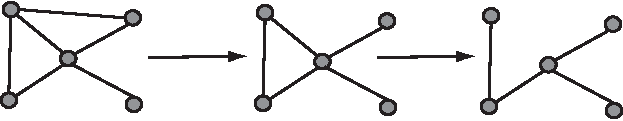
\includegraphics[width=0.6\linewidth]{images/twodeletions}
\caption{Deleting two appropriate edges from this graph gives a spanning tree.\label{twodeletions}}
\end{figure}
\hypertarget{p-667}{}%
The second operation is called \terminology{contraction}.%
\begin{figure}
\centering
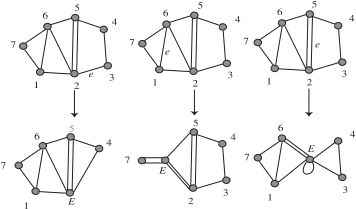
\includegraphics[width=0.65\linewidth]{images/threecontractions}
\caption{The results of contracting three different edges in a graph.\label{threecontractions}}
\end{figure}
\hypertarget{p-668}{}%
Contractions of three different edges in the same graph are shown in \hyperref[threecontractions]{Figure~\ref{threecontractions}}. Intuitively, we contract an edge by shrinking it in length until its endpoints coincide; we let the rest of the graph ``go along for the ride.'' To be more precise, we \terminology{contract}\index{contraction} the edge \(e\) with endpoints \(v\) and \(w\) as follows: \leavevmode%
\begin{enumerate}
\item\hypertarget{li-23}{}\hypertarget{p-669}{}%
remove all edges having either \(v\) or \(w\) or both as an endpoint from the edge set,%
\item\hypertarget{li-24}{}\hypertarget{p-670}{}%
remove \(v\) and \(w\) from the vertex set,%
\item\hypertarget{li-25}{}\hypertarget{p-671}{}%
add a new vertex \(E\) to the vertex set,%
\item\hypertarget{li-26}{}\hypertarget{p-672}{}%
add an edge from \(E\) to each remaining vertex that used to be an endpoint of an edge whose other endpoint was \(v\) or \(w\), and add an edge from \(E\) to \(E\) for any edge other than \(e\) whose endpoints were in the set \(\{v,w\}\).%
\end{enumerate}
%
\par
\hypertarget{p-673}{}%
We use \(G-e\) (read as \(G\) minus \(e\)) to stand for the result of deleting \(e\) from \(G\), and we use \(G/e\) (read as \(G\) contract \(e\)) to stand for the result of contracting \(e\) from \(G\).%
\begin{activity}[]\marginsymbol[-1em]{\pdftooltip{$\importantarrow$\ {\Large$\cdot$}}{especially interesting and essential for this or the next section}} \label{activity-119}
\leavevmode%
\begin{enumerate}[font=\bfseries,label=(\alph*),ref=\alph*]
\item\label{task-99} \marginsymbol[-2.5em]{} \hypertarget{p-674}{}%
How do the number of spanning trees of \(G\) not containing the edge \(e\) and the number of spanning trees of \(G\) containing \(e\) relate to the number of spanning trees of \(G-e\) and \(G/e\)?%
~{\tiny (h)}\item\label{task-100} \marginsymbol[-2.5em]{} \hypertarget{p-676}{}%
Use \(\#(G)\) to stand for the number of spanning trees of \(G\) (so that, for example, \(\#(G/e)\) stands for the number of spanning trees of \(G/e\)). Find an expression for \(\#(G)\) in terms of \(\#(G/e)\) and \(\#(G-e)\). This expression is called the \terminology{deletion-contraction recurrence}\index{deletion-contraction recurrence}\index{recurrence!deletion-contraction}.%
\item\label{task-101} \marginsymbol[-2.5em]{} \hypertarget{p-677}{}%
Use the recurrence of the previous part to compute the number of spanning trees of the graph in \hyperref[spantreeexercise]{Figure~\ref{spantreeexercise}}.%
\begin{figure}
\centering
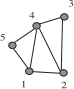
\includegraphics[width=0.2\linewidth]{images/spantreeexercise}
\caption{A graph.\label{spantreeexercise}}
\end{figure}
\end{enumerate}
\end{activity}
\typeout{************************************************}
\typeout{Subsection 2.3.7 Shortest paths in graphs}
\typeout{************************************************}
\subsection[{Shortest paths in graphs}]{Shortest paths in graphs}\label{subsection-27}
\hypertarget{p-681}{}%
Suppose that a company has a main office in one city and regional offices in other cities. Most of the communication in the company is between the main office and the regional offices, so the company wants to find a spanning tree that minimizes not the total cost of all the edges, but rather the cost of communication between the main office and each of the regional offices. It is not clear that such a spanning tree even exists. This problem is a special case of the following. We have a connected graph with nonnegative numbers assigned to its edges. (In this situation these numbers are often called weights.) The \terminology{(weighted) length}\index{path!length of}\index{length (of a path)} of a path in the graph is the sum of the weights of its edges. The \terminology{distance}\index{distance in a weighted graph}\index{graph!distance in} between two vertices is the least (weighted) length of any path between the two vertices. Given a vertex \(v\), we would like to know the distance between \(v\) and each other vertex, and we would like to know if there is a spanning tree in \(G\) such that the length of the path in the spanning tree from \(v\) to each vertex \(x\) is the distance from \(v\) to \(x\) in \(G\).%
\begin{activity}[]\marginsymbol[-1em]{} \label{Dijkstra}
\hypertarget{p-682}{}%
Show that the following algorithm (known as Dijkstra's\index{Dijkstra's algorithm}\index{distance in a graph} algorithm) applied to a weighted graph whose vertices are labelled 1 to \(n\) gives, for each \(i\), the distance from vertex 1 to i as \(d(i)\). \leavevmode%
\begin{enumerate}
\item\hypertarget{li-27}{}\hypertarget{p-683}{}%
Let \(d(1) = 0\). Let \(d(i) = \infty\) for all other \(i\).  Let \(v(1)\)=1. Let \(v(j) = 0\) for all other \(j\).  For each \(i\) and \(j\), let \(w(i,j)\) be the minimum weight of an edge between \(i\) and \(j\), or \(\infty\) if there are no such edges.  Let \(k=1\).  Let \(t=1\).%
\item\hypertarget{li-28}{}\hypertarget{p-684}{}%
For each \(i\), if \(d(i)>d(k) + w(k,i)\) let \(d(i)= d(k) +w(k,i)\).%
\item\hypertarget{li-29}{}\hypertarget{p-685}{}%
Among those \(i\) with \(v(i)=0\), choose one with \(d(i)\) a minimum, and let \(k=i\).  Increase \(t\) by 1. Let \(v(i) =1.\)%
\item\hypertarget{li-30}{}\hypertarget{p-686}{}%
Repeat the previous two steps until \(t=n\)%
\end{enumerate}
%
\end{activity}
\begin{activity}[]\marginsymbol[-1em]{} \label{activity-121}
\hypertarget{p-688}{}%
Is there a spanning tree such that the distance from vertex \(1\) to vertex \(i\) given by the algorithm in \hyperref[Dijkstra]{Problem~\ref{Dijkstra}} is the distance for vertex 1 to vertex \(i\) in the tree (using the same weights on the edges, of course)?%
\end{activity}
\typeout{************************************************}
\typeout{Supplementary Problems 2.4 Supplementary Problems}
\typeout{************************************************}
\section[{Supplementary Problems}]{Supplementary Problems}\label{sec_induction-suppprobs}
\begin{exerciselist}
\item[1.]\marginsymbol[-1em]{} \hypertarget{exercise-13}{}\hypertarget{p-690}{}%
Use the inductive definition of \(a^n\) to prove that \((ab)^n=a^nb^n\) for all nonnegative integers \(n\).%
\par\smallskip
\item[2.]\marginsymbol[-1em]{} \hypertarget{exercise-14}{}\hypertarget{p-693}{}%
Give an inductive definition of \(\displaystyle \bigcup_{i=1}^nS_i\) and use it and the two set distributive law to prove the distributive law \(\displaystyle{A\cap \bigcup_{i=1}^n S_i=\bigcup_{i=1}^n A\cap S_i}\).%
\par\smallskip
\item[3.]\marginsymbol[-1em]{\pdftooltip{$\importantarrow$}{especially interesting}} \hypertarget{exercise-15}{}\hypertarget{p-697}{}%
A hydrocarbon molecule is a molecule whose only atoms are either carbon atoms or hydrogen atoms.  In a simple molecular model of a hydrocarbon, a carbon atom will bond to exactly four other atoms and hydrogen atom will bond to exactly one other atom. Such a model is shown in \hyperref[butane]{Figure~\ref{butane}}. We represent a hydrocarbon compound with a graph whose vertices are labelled with C's and H's so that each C vertex has degree four and each H vertex has degree one.  A hydrocarbon is called an ``alkane'' Common examples are methane (natural gas), butane (one version of which is shown in \hyperref[butane]{Figure~\ref{butane}})propane, hexane (ordinary gasoline), octane (to make gasoline burn more slowly), etc.%
\begin{figure}
\centering
{
\chemfig{H-[:0]C(-[:90]H)(-[:270]H)-[:0]C(-[:90]H)(-[:270]H)-[:0]C(-[:90]H)(-[:270]H)-[:0]C(-[:90]H)(-[:270]H)-[:0]H}
}
\caption{A model of a butane molecule\label{butane}}
\end{figure}
\hypertarget{p-698}{}%
\leavevmode%
\begin{enumerate}[label=(\alph*)]
\item\hypertarget{li-31}{}How many vertices are labelled \(H\) in the graph of an alkane with exactly \(n\) vertices labelled \(C\)?%
\item\hypertarget{li-32}{}An alkane is called butane if it has four carbon atoms. Why do we say one version of butane is shown in \hyperref[butane]{Figure~\ref{butane}}?%
\end{enumerate}
%
\par\smallskip
\item[4.]\marginsymbol[-1em]{} \hypertarget{exercise-16}{}\hypertarget{p-701}{}%
\leavevmode%
\begin{enumerate}[label=(\alph*)]
\item\hypertarget{li-35}{}Give a recurrence for the number of ways to divide \(2n\) people into sets of two for tennis games.  (Don't worry about who serves first.)%
\item\hypertarget{li-36}{}Give a recurrence for the number of ways to divide \(2n\) people into sets of two for tennis games and to determine who serves first.%
\end{enumerate}
%
\par\smallskip
\item[5.]\marginsymbol[-1em]{\pdftooltip{$\importantarrow$}{especially interesting}} \hypertarget{exercise-17}{}\hypertarget{p-704}{}%
Give a recurrence for the number of ways to divide \(4n\) people into sets of four for games of bridge.  (Don't worry about how they sit around the bridge table or who is the first dealer.)%
\par\smallskip
\item[6.]\marginsymbol[-1em]{} \hypertarget{exercise-18}{}\hypertarget{p-706}{}%
Use induction to prove your result in Supplementary \hyperlink{composition_numberof}{Problem~1.4.2} at the end of \hyperref[what-is]{Chapter~\ref{what-is}}.%
\par\smallskip
\item[7.]\marginsymbol[-1em]{} \hypertarget{inductiveprodnotation}{}\hypertarget{p-708}{}%
Give an inductive definition of the product notation \(\displaystyle
\prod_{i=1}^n a_i\).%
\par\smallskip
\item[8.]\marginsymbol[-1em]{} \hypertarget{exercise-20}{}\hypertarget{p-710}{}%
Using the fact that \((ab)^k =a^kb^k\), use your inductive definition of product notation in \hyperlink{inductiveprodnotation}{Problem~2.4.7} to prove that \(\displaystyle \left(\prod_{i=1}^n a_i\right)^k=\prod_{i=1}^n a_i^k\).%
\par\smallskip
\item[9.]\marginsymbol[-1em]{\pdftooltip{$\importantarrow$}{especially interesting}} \hypertarget{exercise-21}{}\hypertarget{p-713}{}%
How many labelled trees on \(n\) vertices have exactly four vertices of degree 1?%
\par\smallskip
\item[10.]\marginsymbol[-1em]{\pdftooltip{$\importantarrow$\ $*$}{especially interesting and difficult}} \hypertarget{exercise-22}{}\hypertarget{p-715}{}%
The \terminology{degree sequence}\index{degree sequence}\index{sequence!degree} of a tree is a list of the degrees of the vertices in nonincreasing order.  For example the degree sequence of the first graph in \hyperref[spanningtrees]{Figure~\ref{spanningtrees}} is \((4,3,2,2,1)\).  For a graph with vertices labeled 1 through \(n\), the \terminology{ordered degree sequence}\index{degree sequence!ordered} of the graph is the sequence \((d_1,d_2,\dots,d_n)\) in which \(d_i\) is the degree of vertex \(i\). For example, the ordered degree sqeuence of the first graph in \hyperref[Threegraphs]{Figure~\ref{Threegraphs}} is \((1,2,3,3,1,1,2,1)\). \leavevmode%
\begin{enumerate}[label=(\alph*)]
\item\hypertarget{li-37}{}How many labelled trees are there on \(n\) vertices with ordered degree sequence \(d_1,d_2,\ldots d_n\)? (This problem appears again in the next chapter since some ideas in that chapter make it more straightforward.)%
\item\hypertarget{li-38}{}How many labeled trees are there on \(n\) vertices with the degree sequence in which the degree \(d\) appears \(i_d\) times?%
\end{enumerate}
%
\par\smallskip
\end{exerciselist}
\typeout{************************************************}
\typeout{Chapter 3 Distribution Problems}
\typeout{************************************************}
\chapter[{Distribution Problems}]{Distribution Problems}\label{ch3-distribution}
\typeout{************************************************}
\typeout{Section 3.1 The idea of a distribution}
\typeout{************************************************}
\section[{The idea of a distribution}]{The idea of a distribution}\label{s3-1-distrib-idea}
\hypertarget{p-719}{}%
Many of the problems we solved in \hyperref[what-is]{Chapter~\ref{what-is}} may be thought of as problems of distributing objects (such as pieces of fruit or ping-pong balls) to recipients (such as children). Some of the ways of viewing counting problems as distribution problems are somewhat indirect. For example, in \hyperref[ping-pong]{Problem~\ref{ping-pong}} you probably noticed that the number of ways to pass out \(k\) ping-pong balls to \(n\) children so that no child gets more than one is the number of ways that we may choose a \(k\)-element subset of an \(n\)-element set. We think of the children as recipients and objects we are distributing as the identical ping-pong balls, distributed so that each recipient gets at most one ball. Those children who receive an object are in our set. It is helpful to have more than one way to think of solutions to problems. In the case of distribution problems, another popular model for distributions is to think of putting balls in boxes rather than distributing objects to recipients. Passing out identical objects is modeled by putting identical balls into boxes. Passing out distinct objects is modeled by putting distinct balls into boxes.%
\typeout{************************************************}
\typeout{Subsection 3.1.1 The twentyfold way}
\typeout{************************************************}
\subsection[{The twentyfold way}]{The twentyfold way}\label{subsection-28}
\hypertarget{p-720}{}%
When we are passing out objects to recipients, we may think of the objects as being either identical or distinct. We may also think of the recipients as being either identical (as in the case of putting fruit into plastic bags in the grocery store) or distinct (as in the case of passing fruit out to children). We may restrict the distributions to those that give at least one object to each recipient, or those that give exactly one object to each recipient, or those that give at most one object to each recipient, or we may have no such restrictions. If the objects are distinct, it may be that the order in which the objects are received is relevant (think about putting books onto the shelves in a bookcase) or that the order in which the objects are received is irrelevant (think about dropping a handful of candy into a child's trick or treat bag). If we ignore the possibility that the order in which objects are received matters, we have created \(2\cdot2\cdot4=16\) distribution problems. In the cases where a recipient can receive more than one distinct object, we also have four more problems when the order objects are received matters. Thus we have 20 possible distribution problems.%
\begin{table}
\centering
\begin{tabular}{ClCcAcC}\hrulethick
\multicolumn{3}{CcC}{The Twentyfold Way: A Table of Distribution Problems}\tabularnewline\hrulethick
\tablecelllines{l}{m}
{\(k\) objects and conditions\\
on how they are received}
&\multicolumn{2}{cC}{\tablecelllines{c}{m}
{\(n\) recipients and mathematical\\
model for distribution}
}\tabularnewline\crulethin{2-3}
&Distinct&Identical\tabularnewline\hrulethick
\tablecelllines{l}{m}
{1.  Distinct\\
no conditions}
&\tablecelllines{c}{m}
{\(n^k\)\\
functions}
&\tablecelllines{c}{m}
{?\\
set partitions (\(\le n\) parts)}
\tabularnewline\hrulethin
\tablecelllines{l}{m}
{2.  Distinct\\
Each gets at most one}
&\tablecelllines{c}{m}
{\(n^{\underline{k}}\)\\
\(k\)-element\\
permutations}
&\tablecelllines{c}{m}
{1 if \(k\le n\);\\
0 otherwise}
\tabularnewline\hrulethin
\tablecelllines{l}{m}
{3.  Distinct\\
Each gets at least one}
&\tablecelllines{c}{m}
{\(?\)\\
onto functions}
&\tablecelllines{c}{m}
{\(?\)\\
set partitions (\(n\) parts)}
\tabularnewline\hrulethin
\tablecelllines{l}{m}
{4. Distinct\\
Each gets exactly one}
&\tablecelllines{c}{m}
{\(k!=n!\)\\
permutations}
&\tablecelllines{c}{m}
{1 if \(k=n\);\\
0 otherwise}
\tabularnewline\hrulethin
\tablecelllines{l}{t}
{5.  Distinct,\\
order matters}
&\tablecelllines{c}{t}
{?\\
?}
&\tablecelllines{c}{t}
{?\\
?}
\tabularnewline\hrulethin
\tablecelllines{l}{t}
{6.  Distinct,\\
order matters\\
Each gets at least one}
&\tablecelllines{c}{t}
{?\\
?}
&\tablecelllines{c}{t}
{?\\
?}
\tabularnewline\hrulethin
\tablecelllines{l}{t}
{7.  Identical\\
no conditions}
&\tablecelllines{c}{t}
{?\\
?}
&\tablecelllines{c}{t}
{?\\
?}
\tabularnewline\hrulethin
\tablecelllines{l}{t}
{8.  Identical\\
Each gets at most one}
&\tablecelllines{c}{t}
{\(\binom{n}{k}\)\\
subsets}
&\tablecelllines{c}{t}
{1 if \(k\le n\);\\
0 otherwise}
\tabularnewline\hrulethin
\tablecelllines{l}{t}
{9.  Identical\\
Each gets at least one}
&\tablecelllines{c}{t}
{?\\
?}
&\tablecelllines{c}{t}
{?\\
?}
\tabularnewline\hrulethin
\tablecelllines{l}{t}
{10.  Identical\\
Each gets exactly one}
&\tablecelllines{c}{t}
{1 if \(k=n\);\\
0 otherwise}
&\tablecelllines{c}{t}
{1 if \(k=n\);\\
0 otherwise}
\tabularnewline\hrulethick
\end{tabular}
\caption{An incomplete table of the number of ways to distribute \(k\) objects to \(n\) recipients, with restrictions on how the objects are received\label{firstdistributiontable}}
\end{table}
\hypertarget{p-721}{}%
We describe these problems in \hyperref[firstdistributiontable]{Table~\ref{firstdistributiontable}}. Since there are twenty possible distribution problems, we call the table the ``Twentyfold Way,''\index{Twentyfold Way} adapting terminology suggested by Joel Spencer for a more restricted class of distribution problems. In the first column of the table we state whether the objects are distinct (like people) or identical (like ping-pong balls) and then give any conditions on how the objects may be received. The conditions we consider are whether each recipient gets at most one object, whether each recipient gets at least one object, whether each recipient gets exactly one object, and whether the order in which the objects are received matters. In the second column we give the solution to the problem and the name of the mathematical model for this kind of distribution problem when the recipients are distinct, and in the third column we give the same information when the recipients are identical. We use question marks as the answers to problems we have not yet solved and models we have not yet studied. We give explicit answers to problems we solved in \hyperref[what-is]{Chapter~\ref{what-is}} and problems whose answers are immediate. The goal of this chapter is to develop methods that will allow us to fill in the table with formulas or at least quantities we know how to compute, and we will give a completed table at the end of the chapter. We will now justify the answers that are not question marks and replace some question marks with answers as we cover relevant material.%
\par
\hypertarget{p-722}{}%
If we pass out \(k\) distinct objects (say pieces of fruit) to \(n\) distinct recipients (say children), we are saying for each object which recipient it goes to. Thus we are defining a function from the set of objects to the recipients. We saw the following theorem in \hyperref[numberoffunctionsconjecture]{Problem~\ref{countingfunctions2}.\ref{numberoffunctionsconjecture}}.%
\begin{theorem}[{}]\label{theorem-3}
\hypertarget{p-723}{}%
There are \(n^k\)\index{functions!number of} functions from a \(k\)-element set to an \(n\)-element set.%
\end{theorem}
\hypertarget{p-724}{}%
We proved it in \hyperref[numberoffunctionsconjecture]{Problem~\ref{countingfunctions2}.\ref{numberoffunctionsconjecture}} and in another way in \hyperref[altproofnumberoffunctionsconjecture]{Problem~\ref{altproofnumberoffunctionsconjecture}}. If we pass out \(k\) distinct objects (say pieces of fruit) to \(n\) indistinguishable recipients (say identical paper bags) then we are dividing the objects up into disjoint sets; that is we are forming a partition of the objects into some number, certainly no more than the number \(k\) of objects, of parts. Later in this chapter (and again in the next chapter) we shall discuss how to compute the number of partitions of a \(k\)-element set into \(n\) parts. This explains the entries in row one of our table.%
\par
\hypertarget{p-725}{}%
If we pass out \(k\) distinct objects to \(n\) recipients so that each gets at most one, we still determine a function, but the function must be one-to-one. The number of one-to-one functions from a \(k\)-element set to an \(n\) element set is the same as the number of one-to-one functions from the set \([k] =\{1,2,\ldots,k\}\) to an \(n\)-element set. In \hyperref[kelementpermutation]{Problem~\ref{kelementpermutation}} we proved the following theorem.%
\begin{theorem}[{}]\label{numberofinjections}
\hypertarget{p-726}{}%
If \(0\le k\le n\), then the number of \(k\)-element permutations of an \(n\)-element set is%
\begin{equation*}
n^{\underline{k}} = n(n-1)\cdots(n-k+1) =
n!/(n-k)!.
\end{equation*}
%
\par
\hypertarget{p-727}{}%
\index{functions!one-to-one!number of}%
\end{theorem}
\hypertarget{p-728}{}%
If \(k>n\) there are no one-to-one functions from a \(k\) element set to an \(n\) element, so we define \(n^{\underline{k}}\) to be zero in this case. Notice that this is what the indicated product in the middle term of our formula gives us. If we are supposed to distribute \(k\) distinct objects to \(n\) identical recipients so that each gets at most one, we cannot do so if \(k>n\), so there are 0 ways to do so. On the other hand, if \(k\le n\), then it doesn't matter which recipient gets which object, so there is only one way to do so. This explains the entries in row two of our table.%
\par
\hypertarget{p-729}{}%
If we distribute \(k\) distinct objects to \(n\) distinct recipients so that each recipient gets at least one, then we are counting functions again, but this time functions from a \(k\)-element set \emph{onto} an \(n\)-element set. At present we do not know how to compute the number of such functions, but we will discuss how to do so later in this chapter and in the next chapter. If we distribute \(k\) identical objects to \(n\) recipients, we are again simply partitioning the objects, but the condition that each recipient gets at least one means that we are partitioning the objects into exactly \(n\) blocks. Again, we will discuss how compute the number of ways of partitioning a set of \(k\) objects into \(n\) blocks later in this chapter. This explains the entries in row three of our table.%
\par
\hypertarget{p-730}{}%
If we pass out \(k\) distinct objects to \(n\) recipients so that each gets exactly one, then \(k=n\) and the function that our distribution gives us is a bijection. The number of bijections from an \(n\)-element set to an \(n\)-element set is \(n!\) by \hyperref[numberofinjections]{Theorem~\ref{numberofinjections}}. If we pass out \(k\) distinct objects of \(n\) identical recipients so that each gets exactly 1, then in this case it doesn't matter which recipient gets which object, so the number of ways to do so is 1 if \(k=n\). If \(k\not=n\), then the number of such distributions is zero. This explains the entries in row four of our table.%
\par
\hypertarget{p-731}{}%
We now jump to row eight of our table. We saw in \hyperref[ping-pong]{Problem~\ref{ping-pong}} that the number of ways to pass out \(k\) identical ping-pong balls to \(n\) children is simply the number of \(k\)-element subsets of an \(n\)-element set. In \hyperref[formulanchoosek]{Problem~\ref{formulanchoosek}} we proved the following theorem.%
\begin{theorem}[{}]\label{theorem-5}
\hypertarget{p-732}{}%
If \(0\le k \le n\), the number of \(k\)-element subsets of an \(n\)-element set is given by%
\begin{equation*}
\binom{n}{k} = \frac{n^{\underline{k}}}{k!}
= \frac{n!}{k!(n-k)!}.
\end{equation*}
%
\end{theorem}
\hypertarget{p-733}{}%
We define \(\binom{n}{k}\) to be 0 if \(k>n\), because then there are no \(k\)-element subsets of an \(n\)-element set. Notice that this is what the middle term of the formula in the theorem gives us. This explains the entries of row 8 of our table. For now we jump over row 9.%
\par
\hypertarget{p-734}{}%
In row 10 of our table, if we are passing out \(k\) identical objects to \(n\) recipients so that each gets exactly one, it doesn't matter whether the recipients are identical or not; there is only one way to pass out the objects if \(k=n\) and otherwise it is impossible to make the distribution, so there are no ways of distributing the objects. This explains the entries of row 10 of our table. Several other rows of our table can be computed using the methods of \hyperref[what-is]{Chapter~\ref{what-is}}.%
\typeout{************************************************}
\typeout{Subsection 3.1.2 Ordered functions}
\typeout{************************************************}
\subsection[{Ordered functions}]{Ordered functions}\label{orderedfunctionsection}
\begin{activity}[]\marginsymbol[-1em]{} \label{bookcase}
\hypertarget{p-735}{}%
Suppose we wish to place \(k\) distinct books onto the shelves of a bookcase with \(n\) shelves. For simplicity, assume for now that all of the books would fit on any of the shelves. Also, let's imagine pushing the books on a shelf as far to the left as we can, so that we are only thinking about how the books sit relative to each other, not about the exact places where we put the books. Since the books are distinct, we can think of a the first book, the second book and so on.%
\begin{enumerate}[font=\bfseries,label=(\alph*),ref=\alph*]
\item\label{task-102} \marginsymbol[-2.5em]{} \hypertarget{p-736}{}%
How many places are there where we can place the first book?%
\item\label{task-103} \marginsymbol[-2.5em]{} \hypertarget{p-738}{}%
When we place the second book, if we decide to place it on the shelf that already has a book, does it matter if we place it to the left or right of the book that is already there?%
\item\label{task-104} \marginsymbol[-2.5em]{} \hypertarget{p-740}{}%
How many places are there where we can place the second book?%
~{\tiny (h)}\item\label{task-105} \marginsymbol[-2.5em]{} \hypertarget{p-743}{}%
Once we have \(i-1\) books placed, if we want to place book \(i\)  on a shelf that already has some books, is sliding it in to the left of all the books already there different from placing it to the right of all the books already or between two books already there?%
\item\label{task-106} \marginsymbol[-2.5em]{} \hypertarget{p-745}{}%
In how many ways may we place the \(i\)th book into the bookcase?%
~{\tiny (h)}\item\label{task-107} \marginsymbol[-2.5em]{} \hypertarget{p-748}{}%
In how many ways may we place all the books?%
\end{enumerate}
\end{activity}
\begin{activity}[]\marginsymbol[-1em]{} \label{bookcaseeveryshelf}
\hypertarget{p-750}{}%
Suppose we wish to place the books in \hyperref[bookcase]{Problem~\ref{bookcase}} (satisfying the assumptions we made there) so that each shelf gets at least one book. Now in how many ways may we place the books? (Hint: how can you make sure that each shelf gets at least one book before you start the process described in \hyperref[bookcase]{Problem~\ref{bookcase}}?)%
~{\tiny (h)}\end{activity}
\hypertarget{p-753}{}%
The assignment of which books go to which shelves of a bookcase is simply a function from the books to the shelves. But a function doesn't determine which book sits to the left of which others on the shelf, and this information is part of how the books are arranged on the shelves. In other words, the order in which the shelves receive their books matters.  Our function must thus assign an ordered list of books to each shelf. We will call such a function an ordered function. More precisely, an \terminology{ordered function}\index{ordered function}\index{function!ordered} from a set \(S\) to a set \(T\) is a function that assigns an (ordered) list of elements of \(S\) to some, but not necessarily all, elements of \(T\) in such a way that each element of \(S\) appears on one and only one of the lists.\footnote{The phrase ordered function is not a standard one, because there is as yet no standard name for the result of an ordered distribution problem.\label{fn-6}} (Notice that although it is not the usual definition of a function from \(S\) to \(T\), a function\index{function!alternate definition} can be described as an assignment of subsets of \(S\) to some, but not necessarily all, elements of \(T\) so that each element of \(S\) is in one and only one of these subsets.) Thus the number of ways to place the books into the bookcase is the entry in the middle column of row 5 of our table. If in addition we require each shelf to get at least one book, we are discussing the entry in the middle column of row 6 of our table. An \terminology{ordered onto function}\index{function!ordered!onto}\index{ordered onto function}\index{onto function!ordered} is one which assigns a list to each element of \(T\). In \hyperref[bookcase]{Problem~\ref{bookcase}} you showed that the number of ordered functions from a \(k\)-element set to an \(n\)-element set is \(\displaystyle \prod_{i=1}^k (n+i-1)\). This product occurs frequently enough that it has a name; it is called the \(k\)\/th \terminology{rising factorial power}\index{factorial power!rising}\index{rising factorial power} of \(n\) and is denoted by \(n^{\overline{k}}\). \index{\(n^{\overline{k}}\)} It is read as ``\(n\) to the \(k\) rising.'' (This notation is due to Don Knuth, who also suggested the notation for falling factorial powers.)\index{factorial} We can summarize with a theorem that adds two more formulas for the number of ordered functions.\index{factorial!falling}\index{falling factorial power}%
\begin{theorem}[{}]\label{theorem-6}
\hypertarget{p-754}{}%
The number of ordered functions from a \(k\)-element set to an \(n\)-element set is%
\begin{equation*}
n^{\overline{k}}=\prod_{i=1}^k (n+i-1) = \frac{(n+i-1)!}{(n-1)!} =
(n+k-1)^{\underline{k}}.
\end{equation*}
%
\end{theorem}
\hypertarget{p-755}{}%
Ordered functions explain the entries in the middle column of rows 5 and 6 of our table of distribution problems.%
\typeout{************************************************}
\typeout{Subsection 3.1.3 Multisets}
\typeout{************************************************}
\subsection[{Multisets}]{Multisets}\label{subsection-30}
\hypertarget{p-756}{}%
In the middle column of row 7 of our table, we are asking for the number of ways to distribute \(k\) identical objects (say ping-pong balls) to \(n\) distinct recipients (say children).%
\begin{activity}[]\marginsymbol[-1em]{\pdftooltip{$\bullet$}{essential}} \label{identicalbooks}
\hypertarget{p-757}{}%
In how many ways may we distribute \(k\) identical books on the shelves of a bookcase with \(n\) shelves, assuming that any shelf can hold all the books?%
~{\tiny (h)}\end{activity}
\begin{activity}[]\marginsymbol[-1em]{\pdftooltip{$\bullet$}{essential}} \label{multiset}
\hypertarget{p-760}{}%
A \terminology{multiset}\index{multiset} chosen from a set \(S\) may be thought of as a subset with repeated elements allowed. For example the multiset of letters of the word Mississippi is \(\{i,i,i,i,m,p,p,s,s,s,s\}\). To determine a multiset we must say how many times (including, perhaps, zero) each member of \(S\) appears in the multiset. The number of times an element appears is called its \terminology{multiplicity}.\index{multiplicity in a multiset} The size of a multiset chosen from \(S\) is the total number of times any member of \(S\) appears. For example, the size of the multiset of letters of Mississippi is 11. What is the number of multisets of size \(k\) that can be chosen from an \(n\)-element set?%
~{\tiny (h)}\end{activity}
\begin{activity}[]\marginsymbol[-1em]{\pdftooltip{$\importantarrow$}{especially interesting}} \label{activity-126}
\hypertarget{p-763}{}%
Your answer in the previous problem should be expressible as a binomial coefficient. Since a binomial coefficient counts subsets, find a bijection between subsets of something and multisets chosen from a set \(S\).%
~{\tiny (h)}\end{activity}
\begin{activity}[]\marginsymbol[-1em]{} \label{activity-127}
\hypertarget{p-766}{}%
How many solutions are there in nonnegative integers to the equation \(x_1+x_2+ \cdots +x_m = r\), where \(m\) and \(r\) are constants?%
~{\tiny (h)}\end{activity}
\begin{activity}[]\marginsymbol[-1em]{} \label{k-obj-n-recip}
\hypertarget{p-769}{}%
In how many ways can we distribute \(k\) identical objects to \(n\) distinct recipients so that each recipient gets at least \(m\)?%
~{\tiny (h)}\end{activity}
\hypertarget{p-772}{}%
Multisets explain the entry in the middle column of row 7 of our table of distribution problems.%
\typeout{************************************************}
\typeout{Subsection 3.1.4 Compositions of integers}
\typeout{************************************************}
\subsection[{Compositions of integers}]{Compositions of integers}\label{subsection-31}
\begin{activity}[]\marginsymbol[-1em]{\pdftooltip{\Large$\cdot$}{essential for this section or the next}} \label{activity-129}
\hypertarget{p-773}{}%
In how many ways may we put \(k\) identical books onto \(n\) shelves if each shelf must get at least one book?%
~{\tiny (h)}\end{activity}
\begin{activity}[]\marginsymbol[-1em]{\pdftooltip{\Large$\cdot$}{essential for this section or the next}} \label{compositionagian}
\hypertarget{p-776}{}%
A \terminology{composition} of the integer \(k\) into \(n\) parts is a list of \(n\) positive integers that add to \(k\).  How many compositions are there of an integer \(k\) into \(n\) parts?%
~{\tiny (h)}\end{activity}
\begin{activity}[]\marginsymbol[-1em]{\pdftooltip{$\importantarrow$}{especially interesting}} \label{activity-131}
\hypertarget{p-779}{}%
Your answer in \hyperref[compositionagian]{Problem~\ref{compositionagian}} can be expressed as a binomial coefficient. This means it should be possible to interpret a composition as a subset of some set. Find a bijection between compositions of \(k\) into \(n\) parts and certain subsets of some set.  Explain explicitly how to get the composition from the subset and the subset from the composition.%
~{\tiny (h)}\end{activity}
\begin{activity}[]\marginsymbol[-1em]{\pdftooltip{\Large$\cdot$}{essential for this section or the next}} \label{activity-132}
\hypertarget{p-782}{}%
Explain the connection between compositions of \(k\) into \(n\) parts and the problem of distributing \(k\) identical objects to \(n\) recipients so that each recipient gets at least one.%
\end{activity}
\hypertarget{p-784}{}%
The sequence of problems you just completed should explain the entry in the middle column of row 9 of our table of distribution problems.%
\typeout{************************************************}
\typeout{Subsection 3.1.5 Broken permutations and Lah numbers}
\typeout{************************************************}
\subsection[{Broken permutations and Lah numbers}]{Broken permutations and Lah numbers}\label{subsection-32}
\begin{activity}[]\marginsymbol[-1em]{\pdftooltip{$\importantarrow$\ {\Large$\cdot$}}{especially interesting and essential for this or the next section}} \label{brokenpermutation}
\hypertarget{p-785}{}%
In how many ways may we stack \(k\) distinct books into \(n\) identical boxes so that there is a stack in every box? The hints may suggest that you can do this problem in more than one way!%
~{\tiny (h)}~{\tiny (h)}\end{activity}
\hypertarget{p-790}{}%
We can think of stacking books into identical boxes as partitioning the books and then ordering the blocks of the partition. This turns out not to be a useful computational way of visualizing the problem because the number of ways to order the books in the various stacks depends on the sizes of the stacks and not just the number of stacks. However this way of thinking actually led to the first hint in \hyperref[brokenpermutation]{Problem~\ref{brokenpermutation}}. Instead of dividing a set up into nonoverlapping parts, we may think of dividing a \emph{permutation} (thought of as a list) of our \(k\) objects up into \(n\) ordered blocks. We will say that a set of ordered lists of elements of a set \(S\) is a \terminology{broken permutation}\index{broken permutation}\index{permutation!broken} of \(S\) if each element of \(S\) is in one and only one of these lists.\footnote{The phrase broken permutation is not standard, because there is no standard name for the solution to this kind  of distribution problem.\label{fn-7}} The number of broken permutations of a \(k\)-element set with \(n\) blocks is denoted by \(L(k,n)\). The number \(L(k,n)\) is called a \terminology{Lah Number} and, from our solution to \hyperref[brokenpermutation]{Problem~\ref{brokenpermutation}}, is equal to \(k!\binom{k-1}{n-1}/n!\).\index{Lah number}%
\par
\hypertarget{p-791}{}%
The Lah numbers are the solution to the question ``In how many ways may we distribute \(k\) distinct objects to \(n\) identical recipients if order matters and each recipient must get at least one?" Thus they give the entry in row 6 and column 3 of our table. The entry in row 5 and column 3 of our table will be the number of broken permutations with less than or equal to \(n\) parts. Thus it is a sum of Lah numbers.%
\par
\hypertarget{p-792}{}%
We have seen that ordered functions and broken permutations explain the entries in rows 5 and 6 of our table.%
\par
\hypertarget{p-793}{}%
In the next two sections we will give ways of computing the remaining entries.%
\typeout{************************************************}
\typeout{Section 3.2 Partitions and Stirling Numbers}
\typeout{************************************************}
\section[{Partitions and Stirling Numbers}]{Partitions and Stirling Numbers}\label{s3-2-partitions}
\hypertarget{p-794}{}%
We have seen how the number of partitions of a set of \(k\) objects into \(n\) blocks corresponds to the distribution of \(k\) distinct objects to \(n\) identical recipients. While there is a formula that we shall eventually learn for this number, it requires more machinery than we now have available. However there is a good method for computing this number that is similar to Pascal's equation. Now that we have studied recurrences in one variable, we will point out that Pascal's equation is in fact a \emph{recurrence in two variables}\index{recurrence!two variable}; that is it lets us compute \(\binom{n}{k}\) in terms of values of \(\binom{m}{i}\) in which either \(m\lt n\) or \(i\lt k\) or both. It was the fact that we had such a recurrence and knew \(\binom{n}{0}\) and \(\binom{n}{n}\) that let us create Pascal's triangle.%
\typeout{************************************************}
\typeout{Subsection 3.2.1 Stirling Numbers of the second kind}
\typeout{************************************************}
\subsection[{Stirling Numbers of the second kind}]{Stirling Numbers of the second kind}\label{subsection-33}
\hypertarget{p-795}{}%
We use the notation \(S(k,n)\) to stand for the number of partitions of a \(k\) element set with \(n\) blocks. For historical reasons, \(S(k,n)\) is called a \terminology{Stirling number of the second kind}. \index{partition!of a set}\index{partition!of a set!!Stirling Numbers}\index{Stirling Number!second kind}\index{\(S(k,n)\)}%
\begin{activity}[]\marginsymbol[-1em]{} \label{secondstirlingrecurrence}
\hypertarget{p-796}{}%
In a partition of the set \([k]\), the number \(k\) is either in a block by itself, or it is not. How does the number of partitions of \([k]\) with \(n\) parts in which \(k\) is in a block with other elements of \([k]\) compare to the number of partitions of \([k-1]\) into \(n\) blocks? Find a two variable recurrence for \(S(n,k)\), valid for \(n\) and \(k\) larger than one.%
~{\tiny (h)}\end{activity}
\begin{activity}[]\marginsymbol[-1em]{} \label{activity-135}
\hypertarget{p-799}{}%
What is \(S(k,1)\)? What is \(S(k,k)\)? Create a table of values of \(S(k,n)\) for \(k\) between 1 and 5 and \(n\) between 1 and \(k\). This table is sometimes called \terminology{Stirling's Triangle (of the second kind)}\index{Stirling's triangle!second kind} How would you define \(S(k,n)\) for the nonnegative values of \(k\) and \(n\) that are not both positive? Now for what values of \(k\) and \(n\) is your two variable recurrence valid?%
\end{activity}
\begin{activity}[]\marginsymbol[-1em]{} \label{sandwiches}
\hypertarget{p-802}{}%
Extend Stirling's triangle enough to allow you to answer the following question and answer it. (Don't fill in the rows all the way; the work becomes quite tedious if you do. Only fill in what you need to answer this question.) A caterer is preparing three bag lunches for hikers. The caterer has nine different sandwiches. In how many ways can these nine sandwiches be distributed into three identical lunch bags so that each bag gets at least one?%
\end{activity}
\begin{activity}[]\marginsymbol[-1em]{} \label{caterer2}
\hypertarget{p-804}{}%
The question in \hyperref[sandwiches]{Problem~\ref{sandwiches}} naturally suggests a more realistic question; in how many ways may the caterer distribute the nine sandwich's into three identical bags so that each bag gets exactly three? Answer this question.%
~{\tiny (h)}\end{activity}
\begin{activity}[]\marginsymbol[-1em]{\pdftooltip{\Large$\cdot$}{essential for this section or the next}} \label{activity-138}
\hypertarget{p-807}{}%
What is \(S(k,k-1)\)?%
~{\tiny (h)}\end{activity}
\begin{activity}[]\marginsymbol[-1em]{\pdftooltip{$\bullet$}{essential}} \label{partitionsgivenpartsize}
\hypertarget{p-810}{}%
In how many ways can we partition \(k\) items into \(n\) blocks so that we have \(k_i\) blocks of size \(i\) for each \(i\)? (Notice that \(\sum_{i=1}^k k_i = n\) and \(\sum_{i=1}^k ik_i = k\).) The sequence \(k_1,k_2,\ldots,k_n\) is called the \terminology{type vector} of the partition.\index{partition of a set!type vector}\index{type vector of a partition of a set}%
~{\tiny (h)}\end{activity}
\begin{activity}[]\marginsymbol[-1em]{\pdftooltip{\tiny$+$}{summary}} \label{activity-140}
\hypertarget{p-813}{}%
Describe how to compute \(S(k,n)\) in terms of quantities given by the formula you found in \hyperref[partitionsgivenpartsize]{Problem~\ref{partitionsgivenpartsize}}.%
\end{activity}
\begin{activity}[]\marginsymbol[-1em]{\pdftooltip{$\importantarrow$}{especially interesting}} \label{activity-141}
\hypertarget{p-815}{}%
Find a recurrence for the Lah numbers \(L(k,n)\) similar to the one in \hyperref[secondstirlingrecurrence]{Problem~\ref{secondstirlingrecurrence}}.%
~{\tiny (h)}\end{activity}
\begin{activity}[]\marginsymbol[-1em]{\pdftooltip{\Large$\cdot$}{essential for this section or the next}} \label{BellNumberIntro}
\hypertarget{p-818}{}%
(Relevant in \hyperref[expogenfun]{Appendix~\ref{expogenfun}}.) The total number of partitions of a \(k\)-element set is denoted by \(B(k)\) and is called the \(k\)-th \terminology{Bell number}\index{Bell Number}\index{partitions of a set!number of}. Thus \(B(1)=1\) and \(B(2) =2\).%
\begin{enumerate}[font=\bfseries,label=(\alph*),ref=\alph*]
\item\label{task-108} \marginsymbol[-2.5em]{} \hypertarget{p-819}{}%
Show, by explicitly exhibiting the partitions, that \(B(3)=5\).%
\item\label{task-109} \marginsymbol[-2.5em]{} \hypertarget{p-821}{}%
Find a recurrence that expresses \(B(k)\) in terms of \(B(n)\) for \(n\lt  k\) and prove your formula correct in as many ways as you can.%
~{\tiny (h)}\item\label{task-110} \marginsymbol[-2.5em]{} \hypertarget{p-825}{}%
Find \(B(k)\) for \(k=4,5,6\).%
\end{enumerate}
\end{activity}
\typeout{************************************************}
\typeout{Subsection 3.2.2 Stirling Numbers and onto functions}
\typeout{************************************************}
\subsection[{Stirling Numbers and onto functions}]{Stirling Numbers and onto functions}\label{subsection-34}
\begin{activity}[]\marginsymbol[-1em]{\pdftooltip{$\circ$}{motivational material}} \label{activity-143}
\hypertarget{p-827}{}%
Given a function \(f\) from a \(k\)-element set \(K\) to an \(n\)-element set, we can define a partition of \(K\) by putting \(x\) and \(y\) in the same block of the partition if and only if \(f(x)=f(y)\). How many blocks does the partition have if \(f\) is onto? How is the number of functions from a \(k\)-element set onto an \(n\)-element set related to a Stirling number? Be as precise in your answer as you can.\index{function!onto!and Stirling Numbers}\index{onto function!counting}%
~{\tiny (h)}\end{activity}
\begin{activity}[]\marginsymbol[-1em]{\pdftooltip{$\importantarrow$}{especially interesting}} \label{activity-144}
\hypertarget{p-830}{}%
How many labeled trees on \(n\) vertices have exactly 3 vertices of degree one?  Note that this problem has appeared before in \hyperref[InductionRecursion]{Chapter~\ref{InductionRecursion}}.%
~{\tiny (h)}\end{activity}
\begin{activity}[]\marginsymbol[-1em]{\pdftooltip{$\bullet$}{essential}} \label{Stirlingfalling}
\hypertarget{p-833}{}%
Each function from a \(k\)-element set \(K\) to an \(n\)-element set \(N\) is a function from \(K\) onto \emph{some} subset of \(N\). If \(J\) is a subset of \(N\) of size \(j\), you know how to compute the number of functions that map onto \(J\) in terms of Stirling numbers. Suppose you add the number of functions mapping onto \(J\) over all possible subsets \(J\) of \(N\). What simple value should this sum equal? Write the equation this gives you.%
~{\tiny (h)}\end{activity}
\begin{activity}[]\marginsymbol[-1em]{\pdftooltip{$\circ$}{motivational material}} \label{activity-146}
\hypertarget{p-836}{}%
In how many ways can the sandwiches of \hyperref[sandwiches]{Problem~\ref{sandwiches}} be placed into three distinct bags so that each bag gets at least one?%
\end{activity}
\begin{activity}[]\marginsymbol[-1em]{\pdftooltip{$\circ$}{motivational material}} \label{activity-147}
\hypertarget{p-838}{}%
In how many ways can the sandwiches of \hyperref[caterer2]{Problem~\ref{caterer2}} be placed into distinct bags so that each bag gets exactly three?%
\end{activity}
\begin{activity}[]\marginsymbol[-1em]{\pdftooltip{$\bullet$}{essential}} \label{activity-148}
\hypertarget{p-841}{}%
In how many ways may we label the elements of a \(k\)-element set with \(n\) distinct labels (numbered 1 through \(n\)) so that label \(i\) is used \(j_i\) times? (If we think of the labels as \(y_1, y_2, \ldots, y_n\), then we can rephrase this question as follows.  How many functions are there from a \(k\)-element set \(K\) to a set \(N=\{y_1,y_2,\ldots y_n\}\) so that \(y_i\) is the image of \(j_i\) elements of \(K\)?) This number is called a \terminology{multinomial coefficient}\index{multinomial coefficient}\index{coefficient!multinomial} and denoted by%
\begin{equation*}
\binom{k}{j_1,j_2,\ldots, j_n}.
\end{equation*}
%
~{\tiny (h)}~{\tiny (h)}\end{activity}
\begin{activity}[]\marginsymbol[-1em]{} \label{activity-149}
\hypertarget{p-845}{}%
Explain how to compute the number of functions from a \(k\)-element set \(K\) to an \(n\)-element set \(N\) by using multinomial coefficients.%
~{\tiny (h)}\end{activity}
\begin{activity}[]\marginsymbol[-1em]{} \label{activity-150}
\hypertarget{p-848}{}%
Explain how to compute the number of functions from a \(k\)-element set \(K\) onto an \(n\)-element set \(N\) by using multinomial coefficients.%
~{\tiny (h)}\end{activity}
\begin{activity}[]\marginsymbol[-1em]{\pdftooltip{$\bullet$}{essential}} \label{activity-151}
\hypertarget{p-851}{}%
What do multinomial coefficients have to do with expanding the \(k\)th power of a multinomial \(x_1+x_2+\cdots+x_n\)? This result is called the \terminology{multinomial theorem}.%
~{\tiny (h)}\end{activity}
\typeout{************************************************}
\typeout{Subsection 3.2.3 Stirling Numbers and bases for polynomials}
\typeout{************************************************}
\subsection[{Stirling Numbers and bases for polynomials}]{Stirling Numbers and bases for polynomials}\label{subsection-35}
\begin{activity}[]\marginsymbol[-1em]{\pdftooltip{\Large$\cdot$}{essential for this section or the next}} \label{powersfromfalling}
\leavevmode%
\begin{enumerate}[font=\bfseries,label=(\alph*),ref=\alph*]
\item\label{task-111} \marginsymbol[-2.5em]{} \hypertarget{p-854}{}%
Find a way to express \(n^k\) in terms of \(k^{\underline{j}}\) for appropriate values \(j\). You may use Stirling numbers if they help you.%
~{\tiny (h)}\item\label{task-112} \marginsymbol[-2.5em]{} \hypertarget{p-857}{}%
Notice that \(x^{\underline{j}}\) makes sense for a numerical variable \(x\) (that could range over the rational numbers, the real numbers, or even the complex numbers instead of only the nonnegative integers, as we are implicitly assuming \(n\) does), just as \(x^j\) does. Find a way to express the power \(x^k\) in terms of the polynomials \(x^{\underline{j}}\) for appropriate values of \(j\) and explain why your formula is correct.%
~{\tiny (h)}\end{enumerate}
\end{activity}
\hypertarget{p-861}{}%
You showed in \hyperref[powersfromfalling]{Problem~\ref{powersfromfalling}} how to get each power of \(x\) in terms of the falling factorial powers \(x^{\underline{j}}\). Therefore every polynomial in \(x\) is expressible in terms of a sum of numerical multiples of falling factorial powers. Using the language of linear algebra, we say that the ordinary powers of \(x\) and the falling factorial powers of \(x\) each form a basis for the ``space'' of polynomials, and that the numbers \(S(k,n)\) are ``change of basis coefficients.'' If you are not familiar with linear algebra, a \terminology{basis}\index{basis (for polynomials)} for the \terminology{space of polynomials}\footnote{The space of polynomials is just another name for the set of all polynomials.\label{fn-8}}\index{space of polynomials} is a set of polynomials such that each polynomial, whether in that set or not, can be expressed in one and only one way as a sum of numerical multiples of polynomials in the set.%
\begin{activity}[]\marginsymbol[-1em]{\pdftooltip{$\circ$}{motivational material}} \label{activity-153}
\hypertarget{p-862}{}%
Show that every power of \(x+1\) is expressible as a sum of numerical multiples of powers of \(x\). Now show that every power of \(x\) (and thus every polynomial in \(x\)) is a sum of numerical multiples (some of which could be negative) of powers of \(x+1\). This means that the powers of \(x+1\) are a basis for the space of polynomials as well. Describe the change of basis coefficients that we use to express the binomial powers \((x+1)^n\) in terms of the ordinary \(x^j\) explicitly. Find the change of basis coefficients we use to express the ordinary powers \(x^n\) in terms of the binomial powers \((x+1)^k\).%
~{\tiny (h)}\end{activity}
\begin{activity}[]\marginsymbol[-1em]{\pdftooltip{$\importantarrow$\ {\Large$\cdot$}}{especially interesting and essential for this or the next section}} \label{Stirlingfirst}
\hypertarget{p-867}{}%
By multiplication, we can see that every falling factorial polynomial can be expressed as a sum of numerical multiples of powers of \(x\). In symbols, this means that there are numbers \(s(k,n)\) (notice that this \(s\) is lower case, not upper case) such that we may write \(x^{\underline{k}} =
\sum_{n=0}^k s(k,n)x^n\). These numbers \(s(k,n)\)\index{\(s(k,n)\)} are called Stirling Numbers of the first kind.\index{Stirling Number!first kind} By thinking algebraically about what the formula%
\begin{equation}
x^{\underline{k}} =
x^{\underline{k-1}}(x-k+1)\label{stirling1}
\end{equation}
means, we can find a recurrence for Stirling numbers of the first kind that gives us another triangular array of numbers called Stirling's triangle of the first kind.\index{Stirling's triangle!first kind} Explain why \hyperref[stirling1]{Equation~(\ref{stirling1})} is true and use it to derive a recurrence for \(s(k,n)\) in terms of \(s(k-1,n-1)\) and \(s(k-1,n)\).%
~{\tiny (h)}~{\tiny (h)}\end{activity}
\begin{activity}[]\marginsymbol[-1em]{} \label{activity-155}
\hypertarget{p-872}{}%
Write down the rows of Stirling's triangle of the first kind for \(k=0\) to~6.%
\end{activity}
\hypertarget{p-873}{}%
By definition, the Stirling numbers of the first kind are also change of basis coefficients. The Stirling numbers of the first and second kind are change of basis coefficients from the falling factorial powers of \(x\) to the ordinary factorial powers, and vice versa.%
\begin{activity}[]\marginsymbol[-1em]{\pdftooltip{$\importantarrow$}{especially interesting}} \label{activity-156}
\hypertarget{p-874}{}%
Explain why every rising factorial polynomial \(x^{\overline{k}}\) can be expressed in terms of the falling factorial polynomials \(x^{\underline{n}}\). Let \(b(k,n)\) stand for the change of basis coefficients that allow us to express \(x^{\overline{k}}\) in terms of the falling factorial polynomials \(x^{\underline{n}}\); that is, define \(b(k,n)\) by the equations%
\begin{equation*}
x^{\overline{k}}=\sum_{n=0}^k b(k,n) x^{\underline{n}}.
\end{equation*}
%
\begin{enumerate}[font=\bfseries,label=(\alph*),ref=\alph*]
\item\label{task-113} \marginsymbol[-2.5em]{} \hypertarget{p-875}{}%
Find a recurrence for \(b(k,n)\).%
~{\tiny (h)}\item\label{task-114} \marginsymbol[-2.5em]{} \hypertarget{p-879}{}%
Find a formula for \(b(k,n)\) and prove the correctness of what you say in as many ways as you can.%
~{\tiny (h)}\item\label{task-115} \marginsymbol[-2.5em]{} \hypertarget{p-883}{}%
Is \(b(k,n)\) the same as any of the other families of numbers (binomial coefficients, Bell numbers, Stirling numbers, Lah numbers, etc.) we have studied?%
\item\label{task-116} \marginsymbol[-2.5em]{} \hypertarget{p-885}{}%
Say as much as you can (but say it precisely) about the change of basis coefficients for expressing \(x^{\underline{k}}\) in terms of \(x^{\overline{n}}\).%
~{\tiny (h)}~{\tiny (h)}\end{enumerate}
\end{activity}
\typeout{************************************************}
\typeout{Section 3.3 Partitions of Integers}
\typeout{************************************************}
\section[{Partitions of Integers}]{Partitions of Integers}\label{s3-3-partitions-int}
\hypertarget{p-890}{}%
We have now completed all our distribution problems except for those in which both the objects and the recipients are identical. For example, we might be putting identical apples into identical paper bags. In this case all that matters is how many bags get one apple (how many recipients get one object), how many get two, how many get three, and so on. Thus for each bag we have a number, and the multiset of numbers of apples in the various bags is what determines our distribution of apples into identical bags. A multiset of positive integers that add to \(n\) is called a \terminology{partition}\index{partition of an integer} of \(n\). Thus the partitions of 3 are 1+1+1, 1+2 (which is the same as 2+1) and 3. The number of partitions of \(k\) is denoted by \(P(k)\); in computing the partitions of 3 we showed that \(P(3) = 3\). It is traditional to use Greek letters like \(\lambda\) (the Greek letter \(\lambda\) is pronounced LAMB duh) to stand for partitons; we might write \(\lambda= 1,1,1\), \(\gamma= 2,1\) and \(\tau = 3\) to stand for the three partitions we just described. We also write \(\lambda = 1^3\) as a shorthand for \(\lambda = 1,1,1\), and we write \(\lambda \dashv 3\) as a shorthand for ``\(\lambda\) is a partition of three."%
\begin{activity}[]\marginsymbol[-1em]{\pdftooltip{$\circ$}{motivational material}} \label{activity-157}
\hypertarget{p-891}{}%
Find all partitions of 4 and find all partitions of 5, thereby computing \(P(4)\) and \(P(5)\).%
\end{activity}
\typeout{************************************************}
\typeout{Subsection 3.3.1 The number of partitions of \(k\) into \(n\) parts}
\typeout{************************************************}
\subsection[{The number of partitions of \(k\) into \(n\) parts}]{The number of partitions of \(k\) into \(n\) parts}\label{subsection-36}
\hypertarget{p-893}{}%
A \terminology{partition of the integer \(k\) into \(n\) parts}\index{partition of an integer!into \(n\) parts} is a multiset of \(n\) positive integers that add to \(k\). We use \(P(k,n)\) to denote the number of partitions of \(k\) into \(n\) parts. Thus \(P(k,n)\) is the number of ways to distribute \(k\) identical objects to \(n\) identical recipients so that each gets at least one.%
\begin{activity}[]\marginsymbol[-1em]{\pdftooltip{$\circ$}{motivational material}} \label{activity-158}
\hypertarget{p-894}{}%
Find \(P(6,3)\) by finding all partitions of 6 into 3 parts. What does this say about the number of ways to put six identical apples into three identical bags so that each bag has at least one apple?%
\end{activity}
\typeout{************************************************}
\typeout{Subsection 3.3.2 Representations of partitions}
\typeout{************************************************}
\subsection[{Representations of partitions}]{Representations of partitions}\label{subsection-37}
\begin{activity}[]\marginsymbol[-1em]{\pdftooltip{$\circ$}{motivational material}} \label{activity-159}
\hypertarget{p-896}{}%
How many solutions are there in the positive integers to the equation \(x_1+x_2+x_3 =7\) with \(x_1\ge x_2\ge x_3\)?%
\end{activity}
\begin{activity}[]\marginsymbol[-1em]{} \label{activity-160}
\hypertarget{p-898}{}%
Explain the relationship between partitions of \(k\) into \(n\) parts and lists \(x_1,x_2\),\textellipsis{}, \(x_n\) of positive integers that add to \(k\) with \(x_1\ge x_2\ge\ldots \ge x_n\). Such a representation of a partition is called a \terminology{decreasing list}\index{partition of an integer!decreasing list} representation of the partition.%
\end{activity}
\begin{activity}[]\marginsymbol[-1em]{\pdftooltip{$\circ$}{motivational material}} \label{activity-161}
\hypertarget{p-900}{}%
Describe the relationship between partitions of \(k\) and lists or vectors \((x_1,x_2,\ldots,x_n)\) such that \(x_1+2x_2+\ldots kx_k = k\).  Such a representation of a partition is called a \terminology{type vector} representation of a partition, and it is typical to leave the trailing zeros out of such a representation; for example \((2,1)\) stands for the same partition as \((2,1,0,0)\). What is the decreasing list representation for this partition, and what number does it partition?\index{partition of an integer!type vector}\index{type vector for a partition of an integer}%
\end{activity}
\begin{activity}[]\marginsymbol[-1em]{} \label{activity-162}
\hypertarget{p-902}{}%
How does the number of partitions of \(k\) relate to the number of partitions of \(k+1\) whose smallest part is one?%
~{\tiny (h)}\end{activity}
\hypertarget{p-905}{}%
When we write a partition as \(\lambda = \lambda_1,\lambda_2,\ldots,\lambda_n\), it is customary to write the list of \(\lambda_i\)s as a decreasing list. When we have a type vector \((t_1,t_2,\ldots,t_m)\) for a partition, we write either \(\lambda = 1^{t_1}2^{t_2}\cdots m^{t_m}\) or \(\lambda = m^{t_m}(m-1)^{t_{m-1}}\cdots 2^{t_2}1^{t_1}\). Henceforth we will use the second of these. When we write \(\lambda=\lambda_1^{i_1}\lambda_2^{i_2}\cdots\lambda_n^{i_n}\), we will assume that \(\lambda_i>\lambda_{i+1}\).%
\typeout{************************************************}
\typeout{Subsection 3.3.3 Ferrers and Young Diagrams and the conjugate of a partition}
\typeout{************************************************}
\subsection[{Ferrers and Young Diagrams and the conjugate of a partition}]{Ferrers and Young Diagrams and the conjugate of a partition}\label{subsection-38}
\hypertarget{p-906}{}%
The decreasing list representation of partitions leads us to a handy way to visualize partitions. Given a decreasing list \((\lambda_1,\lambda_2,\ldots \lambda_n)\), we draw a figure made up of rows of dots that has \(\lambda_1\) equally spaced dots in the first row, \(\lambda_2\) equally spaced dots in the second row, starting out right below the beginning of the first row and so on. Equivalently, instead of dots, we may use identical squares, drawn so that a square touches each one to its immediate right or immediately below it along an edge. See \hyperref[FerrersYoung]{Figure~\ref{FerrersYoung}} for examples.\index{Ferrers diagram}\index{Young diagram}\index{partition of an integer!Ferrers diagram}\index{partition of an integer!Young diagram}\index{diagram!of a partition!Ferrers}\index{diagram!of a partition!Young} The figure we draw with dots is called the \terminology{Ferrers diagram} of the partition; sometimes the figure with squares is also called a Ferrers diagram; sometimes it is called a \terminology{Young diagram}. At this stage it is irrelevant which name we choose and which kind of figure we draw; in more advanced work the squares are handy because we can put things like numbers or variables into them.  From now on we will use squares and call the diagrams Young diagrams.%
\begin{figure}
\centering
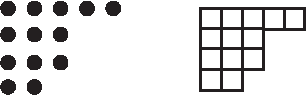
\includegraphics[width=0.45\linewidth]{images/FerrersYoung}
\caption{The Ferrers and Young diagrams of the partition (5,3,3,2)\label{FerrersYoung}}
\end{figure}
\begin{activity}[]\marginsymbol[-1em]{\pdftooltip{$\bullet$}{essential}} \label{activity-163}
\hypertarget{p-907}{}%
Draw the Young diagram of the partition (4,4,3,1,1). Describe the geometric relationship between the Young diagram of (5,3,3,2) and the Young diagram of (4,4,3,1,1).%
~{\tiny (h)}\end{activity}
\begin{activity}[]\marginsymbol[-1em]{\pdftooltip{$\bullet$}{essential}} \label{activity-164}
\hypertarget{p-910}{}%
The partition \((\lambda_1,\lambda_2,\ldots, \lambda_n)\) is called the \terminology{conjugate}\index{conjugate of an integer partition}\index{partition of an integer!conjugate of} of the partition \((\gamma_1,\gamma_2,\ldots, \gamma_m)\) if we obtain the Young diagram of one from the Young diagram of the other by flipping one around the line with slope -1 that extends the diagonal of the top left square. See \hyperref[conjugateYoung]{Figure~\ref{conjugateYoung}} for an example.%
\begin{figure}
\centering
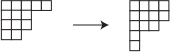
\includegraphics[width=0.5\linewidth]{images/conjugateYoung}
\caption{The Ferrers diagram the partition (5,3,3,2) and its conjugate.\label{conjugateYoung}}
\end{figure}
\hypertarget{p-911}{}%
What is the conjugate of (4,4,3,1,1)? How is the largest part of a partition related to the number of parts of its conjugate? What does this tell you about the number of partitions of a positive integer \(k\) with largest part \(m\)?%
~{\tiny (h)}\end{activity}
\begin{activity}[]\marginsymbol[-1em]{\pdftooltip{$\importantarrow$}{especially interesting}} \label{activity-165}
\hypertarget{p-914}{}%
A partition is called \terminology{self-conjugate}\index{self-conjugate partition}\index{partition of an integer!self conjugate} if it is equal to its conjugate. Find a relationship between the number of self-conjugate partitions of \(k\) and the number of partitions of \(k\) into distinct odd parts.%
~{\tiny (h)}\end{activity}
\begin{activity}[]\marginsymbol[-1em]{} \label{partition-even-mult-even-use}
\hypertarget{p-918}{}%
Explain the relationship between the number of partitions of \(k\) into even parts and the number of partitions of \(k\) into parts of even multiplicity, i.e. parts which are each used an even number of times as in (3,3,3,3,2,2,1,1).%
~{\tiny (h)}\end{activity}
\begin{activity}[]\marginsymbol[-1em]{\pdftooltip{$\importantarrow$}{especially interesting}} \label{rectanglecomplement}
\hypertarget{p-921}{}%
Show that the number of partitions of \(k\) into four parts equals the number of partitions of \(3k\) into four parts of size at most \(k-1\) (or \(3k-4\) into four parts of size at most \(k-2\) or \(3k-4\) into four parts of size at most \(k\)).%
~{\tiny (h)}\end{activity}
\begin{activity}[]\marginsymbol[-1em]{} \label{activity-168}
\hypertarget{p-924}{}%
The idea of conjugation of a partition could be defined without the geometric interpretation of a Young diagram, but it would seem far less natural without the geometric interpretation. Another idea that seems much more natural in a geometric context is this. Suppose we have a partition of \(k\) into \(n\) parts with largest part \(m\). Then the Young diagram of the partition can fit into a rectangle that is \(m\) or more units wide (horizontally) and \(n\) or more units deep. Suppose we place the Young diagram of our partition in the top left-hand corner of an \(m'\) unit wide and \(n'\) unit deep rectangle with \(m'\ge m\) and \(n' \ge n\), as in \hyperref[complementpartition]{Figure~\ref{complementpartition}}.%
\begin{figure}
\centering
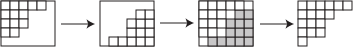
\includegraphics[width=0.7\linewidth]{images/complementpartition}
\caption{To complement the partition \((5,3,3,2)\) in a 6 by 5 rectangle: enclose it in the rectangle, rotate, and cut out the original Young diagram.\label{complementpartition}}
\end{figure}
\begin{enumerate}[font=\bfseries,label=(\alph*),ref=\alph*]
\item\label{task-117} \marginsymbol[-2.5em]{} \hypertarget{p-925}{}%
Why can we interpret the part of the rectangle not occupied by our Young diagram, rotated in the plane, as the Young diagram of another partition? This is called the \terminology{complement}\index{complement of a partition} of our partition in the rectangle.%
\item\label{task-118} \marginsymbol[-2.5em]{} \hypertarget{p-927}{}%
What integer is being partitioned by the complement?%
\item\label{task-119} \marginsymbol[-2.5em]{} \hypertarget{p-929}{}%
What conditions on \(m'\) and \(n'\) guarantee that the complement has the same number of parts as the original one?%
~{\tiny (h)}\item\label{task-120} \marginsymbol[-2.5em]{} \hypertarget{p-932}{}%
What conditions on \(m'\) and \(n'\) guarantee that the complement has the same largest part as the original one?%
~{\tiny (h)}\item\label{task-121} \marginsymbol[-2.5em]{} \hypertarget{p-935}{}%
Is it possible for the complement to have both the same number of parts and the same largest part as the original one?%
\item\label{task-122} \marginsymbol[-2.5em]{} \hypertarget{p-937}{}%
If we complement a partition in an \(m'\) by \(n'\) box and then complement that partition in an \(m'\) by \(n'\) box again, do we get the same partition that we started with?%
\end{enumerate}
\end{activity}
\begin{activity}[]\marginsymbol[-1em]{\pdftooltip{$\importantarrow$}{especially interesting}} \label{activity-169}
\hypertarget{p-939}{}%
Suppose we take a partition of \(k\) into \(n\) parts with largest part \(m\), complement it in the smallest rectangle it will fit into, complement the result in the smallest rectangle it will fit into, and continue the process until we get the partition 1 of one into one part.  What can you say about the partition with which we started?%
~{\tiny (h)}~{\tiny (h)}\end{activity}
\begin{activity}[]\marginsymbol[-1em]{} \label{activity-170}
\hypertarget{p-946}{}%
Show that \(P(k,n)\) is at least \(\frac{1}{n!}\binom{k-1}{n-1}\).%
~{\tiny (h)}\end{activity}
\hypertarget{p-949}{}%
With the binomial coefficients, with Stirling numbers of the second kind, and with the Lah numbers, we were able to find a recurrence by asking what happens to our subset, partition, or broken permutation of a set \(S\) of numbers if we remove the largest element of \(S\). Thus it is natural to look for a recurrence to count the number of partitions of \(k\) into \(n\) parts by doing something similar. Unfortunately, since we are counting distributions in which all the objects are identical, there is no way for us to identify a largest element. However if we think geometrically, we can ask what we could remove from a Young diagram to get a Young diagram. Two natural ways to get a partition of a smaller integer from a partition of \(n\) would be to remove the top row of the Young diagram of the partition and to remove the left column of the Young diagram of the partition. These two operations correspond to removing the largest part from the partition and to subtracting 1 from each part of the partition respectively. Even though they are symmetric with respect to conjugation, they aren't symmetric with respect to the number of parts. Thus one might be much more useful than the other for finding a recurrence for the number of partitions of \(k\) into \(n\) parts.%
\begin{activity}[]\marginsymbol[-1em]{\pdftooltip{$\importantarrow$\ {\Large$\cdot$}}{especially interesting and essential for this or the next section}} \label{numberpartitionrecurrence}
\hypertarget{p-950}{}%
In this problem we will study the two operations and see which one seems more useful for getting a recurrence for \(P(k,n)\).%
\begin{enumerate}[font=\bfseries,label=(\alph*),ref=\alph*]
\item\label{task-123} \marginsymbol[-2.5em]{} \hypertarget{p-951}{}%
How many parts does the remaining partition have when we remove the largest part (more precisely, we reduce its multiplicity by one) from a partition of \(k\) into \(n\) parts?  What can you say about the number of parts of the remaining partition if we remove one from each part?%
~{\tiny (h)}\item\label{task-124} \marginsymbol[-2.5em]{} \hypertarget{p-954}{}%
If we remove the largest part from a partition, what can we say about the integer that is being partitioned by the remaining parts of the partition? If we remove one from each part of a partition of \(k\) into \(n\) parts, what integer is being partitioned by the remaining parts? (Another way to describe this is that we remove the first column from the Young diagram of the partition.)%
~{\tiny (h)}\item\label{task-125} \marginsymbol[-2.5em]{} \hypertarget{p-957}{}%
The last two questions are designed to get you thinking about how we can get a bijection between the set of partitions of \(k\) into \(n\) parts and some other set of partitions that are partitions of a smaller number.  These questions describe two different strategies for getting that set of partitions of a smaller number or of smaller numbers.  Each strategy leads to a bijection between partitions of \(k\) into \(n\) parts and a set of partitions of a smaller number or numbers.  For each strategy, use the answers to the last two questions to find and describe this set of partitions into a smaller number and a bijection between partitions of \(k\) into \(n\) parts and partitions of the smaller integer or integers into appropriate numbers of parts. (In one case the set of partitions and bijection are relatively straightforward to describe and in the other case not so easy.)%
~{\tiny (h)}\item\label{task-126} \marginsymbol[-2.5em]{} \hypertarget{p-961}{}%
Find a recurrence (which need not have just two terms on the right hand side) that describes how to compute \(P(k,n)\) in terms of the number of partitions of smaller integers into a smaller number of parts.%
~{\tiny (h)}\item\label{task-127} \marginsymbol[-2.5em]{} \hypertarget{p-964}{}%
What is \(P(k,1)\) for a positive integer \(k\)?%
\item\label{task-128} \marginsymbol[-2.5em]{} \hypertarget{p-966}{}%
What is \(P(k,k)\) for a positive integer \(k\)?%
\item\label{task-129} \marginsymbol[-2.5em]{} \hypertarget{p-968}{}%
Use your recurrence to compute a table with the values of \(P(k,n)\) for values of \(k\) between 1 and 7.%
\item\label{task-130} \marginsymbol[-2.5em]{} \hypertarget{p-969}{}%
What would you want to fill into row 0 and column 0 of your table in order to make it consistent with your recurrence.  What does this say \(P(0,0)\) should be?  We usually define a sum with no terms in it to be zero. Is that consistent with the way the recurrence says we should define \(P(0,0)\)?%
~{\tiny (h)}\end{enumerate}
\end{activity}
\hypertarget{p-972}{}%
It is remarkable that there is no known formula for \(P(k,n)\), nor is there one for \(P(k)\). This section was are devoted to developing methods for computing values of \(P(n,k)\) and finding properties of \(P(n,k)\) that we can prove even without knowing a formula. Some future sections will attempt to develop other methods.%
\par
\hypertarget{p-973}{}%
We have seen that the number of partitions of \(k\) into \(n\) parts is equal to the number of ways to distribute \(k\) identical objects to \(n\) recipients so that each receives at least one. If we relax the condition that each recipient receives at least one, then we see that the number of distributions of \(k\) identical objects to \(n\) recipients is \(\sum_{i=1}^n P(k,i)\) because if some recipients receive nothing, it does not matter which recipients these are. This completes rows 7 and 8 of our table of distribution problems. The completed table is shown in \hyperref[lastdistributiontable]{Table~\ref{lastdistributiontable}}. There are quite a few theorems that you have proved which are summarized by \hyperref[lastdistributiontable]{Table~\ref{lastdistributiontable}}.  It would be worthwhile to try to write them all down!%
\begin{table}
\centering
\begin{tabular}{ClCcAcC}\hrulethick
\multicolumn{3}{CcC}{The Twentyfold Way: A Table of Distribution Problems}\tabularnewline\hrulethick
\tablecelllines{l}{m}
{\(k\) objects and conditions\\
on how they are received}
&\multicolumn{2}{cC}{\tablecelllines{c}{m}
{\(n\) recipients and mathematical\\
model for distribution}
}\tabularnewline\crulethin{2-3}
&Distinct&Identical\tabularnewline\hrulethick
\tablecelllines{l}{m}
{1.  Distinct\\
no conditions}
&\tablecelllines{c}{m}
{\(n^k\)\\
functions}
&\tablecelllines{c}{m}
{\(\sum_{i=1}^kS(n,i)\)\\
set partitions (\(\le n\) parts)}
\tabularnewline\hrulethin
\tablecelllines{l}{m}
{2.  Distinct\\
Each gets at most one}
&\tablecelllines{c}{m}
{\(n^{\underline{k}}\)\\
\(k\)-element\\
permutations}
&\tablecelllines{c}{m}
{1 if \(k\le n\);\\
0 otherwise}
\tabularnewline\hrulethin
\tablecelllines{l}{m}
{3.  Distinct\\
Each gets at least one}
&\tablecelllines{c}{m}
{\(S(k,n)n!\)\\
onto functions}
&\tablecelllines{c}{m}
{\(S(k,n)\)\\
set partitions (\(n\) parts)}
\tabularnewline\hrulethin
\tablecelllines{l}{m}
{4. Distinct\\
Each gets exactly one}
&\tablecelllines{c}{m}
{\(k!=n!\)\\
permutations}
&\tablecelllines{c}{m}
{1 if \(k=n\);\\
0 otherwise}
\tabularnewline\hrulethin
\tablecelllines{l}{t}
{5.  Distinct,\\
order matters}
&\tablecelllines{c}{t}
{\((k+n-1)^{\underline{k}}\)\\
ordered functions}
&\tablecelllines{c}{t}
{\(\sum_{i=1}^n L(k,i)\)\\
broken permutations\\
(\(\le n\) parts)}
\tabularnewline\hrulethin
\tablecelllines{l}{t}
{6.  Distinct,\\
order matters\\
Each gets at least one}
&\tablecelllines{c}{t}
{\((k)^{\underline{n}}(k-1)^{\underline{k-n}}\)\\
ordered\\
onto functions}
&\tablecelllines{c}{t}
{\(L(k,n)= \binom{k}{n}(k-1)^{\underline{k-n}}\)\\
broken permutations\\
(\(n\) parts)}
\tabularnewline\hrulethin
\tablecelllines{l}{t}
{7.  Identical\\
no conditions}
&\tablecelllines{c}{t}
{\(\binom{n+k-1}{k}\)\\
multisets}
&\tablecelllines{c}{t}
{\(\sum_{i=1}^nP(k,i)\)\\
number partitions\\
(\(\le n\) parts)}
\tabularnewline\hrulethin
\tablecelllines{l}{t}
{8.  Identical\\
Each gets at most one}
&\tablecelllines{c}{t}
{\(\binom{n}{k}\)\\
subsets}
&\tablecelllines{c}{t}
{1 if \(k\le n\);\\
0 otherwise}
\tabularnewline\hrulethin
\tablecelllines{l}{t}
{9.  Identical\\
Each gets at least one}
&\tablecelllines{c}{t}
{\(\binom{k-1}{n-1}\)\\
compositions\\
(\(n\) parts)}
&\tablecelllines{c}{t}
{\(P(k,n)\)\\
number partitions\\
(\(n\) parts)}
\tabularnewline\hrulethin
\tablecelllines{l}{t}
{10.  Identical\\
Each gets exactly one}
&\tablecelllines{c}{t}
{1 if \(k=n\);\\
0 otherwise}
&\tablecelllines{c}{t}
{1 if \(k=n\);\\
0 otherwise}
\tabularnewline\hrulethick
\end{tabular}
\caption{The number of ways to distribute \(k\) objects to \(n\) recipients, with restrictions on how the objects are received\label{lastdistributiontable}}
\end{table}
\typeout{************************************************}
\typeout{Subsection 3.3.4 Partitions into distinct parts}
\typeout{************************************************}
\subsection[{Partitions into distinct parts}]{Partitions into distinct parts}\label{subsection-39}
\hypertarget{p-974}{}%
Often \(Q(k,n)\) is used to denote the number of partitions of \(k\) into distinct parts, that is, parts that are different from each other.%
\begin{activity}[]\marginsymbol[-1em]{} \label{activity-172}
\hypertarget{p-975}{}%
Show that%
\begin{equation*}
Q(k,n) \le \frac{1}{n!}\binom{k-1}{n-1}.
\end{equation*}
%
~{\tiny (h)}\end{activity}
\begin{activity}[]\marginsymbol[-1em]{\pdftooltip{$\importantarrow$}{especially interesting}} \label{activity-173}
\hypertarget{p-978}{}%
Show that the number of partitions of 7 into 3 parts equals the number of partitions of 10 into three distinct parts.%
~{\tiny (h)}\end{activity}
\begin{activity}[]\marginsymbol[-1em]{\pdftooltip{$\importantarrow$\ {\Large$\cdot$}}{especially interesting and essential for this or the next section}} \label{activity-174}
\hypertarget{p-981}{}%
There is a relationship between \(P(k,n)\) and \(Q(m,n)\) for some other number \(m\). Find the number \(m\) that gives you the nicest possible relationship.%
~{\tiny (h)}\end{activity}
\begin{activity}[]\marginsymbol[-1em]{\pdftooltip{\Large$\cdot$}{essential for this section or the next}} \label{activity-175}
\hypertarget{p-984}{}%
Find a recurrence that expresses \(Q(k,n)\) as a sum of \(Q(k-n,m)\) for appropriate values of \(m\).%
~{\tiny (h)}\end{activity}
\begin{activity}[]\marginsymbol[-1em]{\pdftooltip{$\importantarrow$\ $*$}{especially interesting and difficult}} \label{activity-176}
\hypertarget{p-987}{}%
Show that the number of partitions of \(k\) into distinct parts equals the number of partitions of \(k\) into odd parts.%
~{\tiny (h)}\end{activity}
\begin{activity}[]\marginsymbol[-1em]{\pdftooltip{$\importantarrow$\ $*$}{especially interesting and difficult}} \label{activity-177}
\hypertarget{p-991}{}%
Euler showed that if \(k\not= \frac{3j^2+j}{2}\), then the number of partitions of \(k\) into an even number of distinct parts is the same as the number of partitions of \(k\) into an odd number of distinct parts. Prove this, and in the exceptional case find out how the two numbers relate to each other.%
~{\tiny (h)}\end{activity}
\typeout{************************************************}
\typeout{Supplementary Problems 3.4 Supplementary Problems}
\typeout{************************************************}
\section[{Supplementary Problems}]{Supplementary Problems}\label{sec_distribution-suppprobs}
\begin{exerciselist}
\item[1.]\marginsymbol[-1em]{} \hypertarget{exercise-23}{}\hypertarget{p-998}{}%
Answer each of the following questions with \(n^k\), \(k^n\), \(n!\), \(k!\), \(\binom{n}{k}\), \(\binom{k}{n}\), \(n^{\underline{k}}\), \(k^{\underline{n}}\), \(n^{\overline{k}}\), \(k^{\overline{n}}\), \(\binom{n+k-1}{k}\), \(\binom{n+k-1}{n}\), \(\binom{n-1}{k-1}\), \(\binom{k-1}{n-1}\), or ``none of the above". \leavevmode%
\begin{enumerate}[label=(\alph*)]
\item\hypertarget{li-41}{}\hypertarget{p-999}{}%
In how many ways may we pass out \(k\) identical pieces of candy to \(n\) children?%
\item\hypertarget{li-42}{}\hypertarget{p-1000}{}%
In how many ways may we pass out \(k\) distinct pieces of candy to \(n\) children?%
\item\hypertarget{li-43}{}\hypertarget{p-1001}{}%
In how many ways may we pass out \(k\) identical pieces of candy to \(n\) children so that each gets at most one?  (Assume \(k\le n\).)%
\item\hypertarget{li-44}{}\hypertarget{p-1002}{}%
In how many ways may we pass out \(k\) distinct pieces of candy to \(n\) children so that each gets at most one?  (Assume \(k\le n\).)%
\item\hypertarget{li-45}{}\hypertarget{p-1003}{}%
In how many ways may we pass out \(k\) distinct pieces of candy to \(n\) children so that each gets at least one?  (Assume \(k\ge n\).)%
\item\hypertarget{li-46}{}\hypertarget{p-1004}{}%
In how many ways may we pass out \(k\) identical pieces of candy to \(n\) children so that each gets at least one?  (Assume \(k\ge n\).)%
\end{enumerate}
%
\par\smallskip
\item[2.]\marginsymbol[-1em]{} \hypertarget{exercise-24}{}\hypertarget{p-1006}{}%
The neighborhood betterment committee has been given \(r\) trees to distribute to \(s\) families living along one side of a street. \leavevmode%
\begin{enumerate}[label=(\alph*)]
\item\hypertarget{li-53}{}\hypertarget{p-1007}{}%
In how many ways can they distribute all of them if the trees are distinct, there are more families than trees, and each family can get at most one?%
\item\hypertarget{li-54}{}\hypertarget{p-1008}{}%
In how many ways can they distribute all of them if the trees are distinct, any family can get any number, and a family may plant its trees where it chooses?%
\item\hypertarget{li-55}{}\hypertarget{p-1009}{}%
In how many ways can they distribute all the trees if the trees are identical, there are no more trees than families,   and any family receives at most one?%
\item\hypertarget{li-56}{}\hypertarget{p-1010}{}%
In how many ways can they distribute them if the trees are distinct, there are more trees than families, and each family receives at most one (so there could be some leftover trees)?%
\item\hypertarget{multisetproblem}{}\hypertarget{p-1011}{}%
In how many ways can they distribute all the trees if they are identical and anyone may receive any number of trees?%
\item\hypertarget{orderedfunctionproblem}{}\hypertarget{p-1012}{}%
In how many ways can all the trees be distributed and planted if the trees are distinct, any family can get any number, and a family must plant its trees in an evenly spaced row along the road?%
\item\hypertarget{li-59}{}\hypertarget{p-1013}{}%
Answer the question in \hyperlink{orderedfunctionproblem}{Part~3.4.2.f} assuming that every family must get a tree.%
\item\hypertarget{li-60}{}\hypertarget{p-1014}{}%
Answer the question in \hyperlink{multisetproblem}{Part~3.4.2.e} assuming that each family must get at least one tree.%
\end{enumerate}
%
\par\smallskip
\item[3.]\marginsymbol[-1em]{} \hypertarget{exercise-25}{}\hypertarget{p-1016}{}%
In how many ways can \(n\) identical chemistry books, \(r\) identical mathematics books, \(s\) identical physics books, and \(t\) identical astronomy books be arranged on three bookshelves?  (Assume there is no limit on the number of books per shelf.)%
\par\smallskip
\item[4.]\marginsymbol[-1em]{\pdftooltip{$\importantarrow$}{especially interesting}} \hypertarget{exercise-26}{}\hypertarget{p-1018}{}%
One formula for the Lah numbers is%
\begin{equation*}
L(k,n) = \binom{k}{n}(k-1)^{\underline{k-n}}
\end{equation*}
Find a proof that explains this product.%
\par\smallskip
\item[5.]\marginsymbol[-1em]{} \hypertarget{exercise-27}{}\hypertarget{p-1020}{}%
What is the number of partitions of \(n\) into two parts?%
\par\smallskip
\item[6.]\marginsymbol[-1em]{} \hypertarget{partitions-k-2-parts}{}\hypertarget{p-1022}{}%
What is the number of partitions of \(k\) into \(k - 2\) parts?%
\par\smallskip
\item[7.]\marginsymbol[-1em]{} \hypertarget{exercise-29}{}\hypertarget{p-1024}{}%
Show that the number of partitions of \(k\) into \(n\) parts of size at most \(m\) equals the number of partitions of \(mn-k\) into no more than \(n\) parts of size at most \(m-1\).%
\par\smallskip
\item[8.]\marginsymbol[-1em]{} \hypertarget{exercise-30}{}\hypertarget{p-1026}{}%
Show that the number of partitions of \(k\) into parts of size at most \(m\) is equal to the number of partitions of of \(k+m\) into \(m\) parts.%
\par\smallskip
\item[9.]\marginsymbol[-1em]{} \hypertarget{exercise-31}{}\hypertarget{p-1028}{}%
You can say something pretty specific about self-conjugate partitions of \(k\) into distinct parts.  Figure out what it is and prove it.  With that, you should be able to find a relationship between these partitions and partitions whose parts are consecutive integers, starting with 1.  What is that relationship?%
\par\smallskip
\item[10.]\marginsymbol[-1em]{} \hypertarget{exercise-32}{}\hypertarget{p-1030}{}%
What is \(s(k,1)\)?%
\par\smallskip
\item[11.]\marginsymbol[-1em]{} \hypertarget{exercise-33}{}\hypertarget{p-1032}{}%
Show that the Stirling numbers of the second kind satisfy the recurrence%
\begin{equation*}
S(k,n) = \sum_{i=1}^kS(k-i,n-1)\binom{n-1}{i-1}\text{.}
\end{equation*}
%
\par\smallskip
\item[12.]\marginsymbol[-1em]{\pdftooltip{$\importantarrow$}{especially interesting}} \hypertarget{exercise-34}{}\hypertarget{p-1034}{}%
Let \(c(k,n)\) be the number of ways for \(k\) children to hold hands to form \(n\) circles, where one child clasping his or her hands together and holding them out to form a circle is considered a circle.  Find a recurrence for \(c(k,n)\).  Is the family of numbers \(c(k,n)\) related to any of the other families of numbers we have studied? If so, how?%
\par\smallskip
\item[13.]\marginsymbol[-1em]{\pdftooltip{$\importantarrow$}{especially interesting}} \hypertarget{exercise-35}{}\hypertarget{p-1036}{}%
How many labeled trees on \(n\) vertices have exactly four vertices of degree 1?%
\par\smallskip
\item[14.]\marginsymbol[-1em]{\pdftooltip{$\importantarrow$}{especially interesting}} \hypertarget{exercise-36}{}\hypertarget{p-1038}{}%
The \terminology{degree sequence}\index{degree sequence} of a graph is a list of the degrees of the vertices in non-increasing order. For example the degree sequence of the first graph in \hyperref[spanningtrees]{Figure~\ref{spanningtrees}} is \((4, 3, 2, 2, 1)\). For a graph with vertices labeled 1 through \(n\), the \terminology{ordered degree sequence}\index{ordered degree sequence} of the graph is the sequence \(d_1, d_2,\dots, d_n\) in which \(d_i\) is the degree of vertex \(i\). For example the ordered degree sequence of the first graph in \hyperref[Threegraphs]{Figure~\ref{Threegraphs}} is \((1,2,3,3,1,1,2,1)\).%
\par
\hypertarget{p-1039}{}%
\leavevmode%
\begin{enumerate}[label=(\alph*)]
\item\hypertarget{li-69}{}\hypertarget{p-1040}{}%
How many labeled trees are there on \(n\) vertices with ordered degree sequence \(d_1, d_2, \dots, d_n\)?%
\item\hypertarget{li-70}{}\hypertarget{p-1041}{}%
How many labeled trees are there on \(n\) vertices with with the degree sequence in which the degree \(d\) appears \(i_d\) times?%
\end{enumerate}
%
\par\smallskip
\end{exerciselist}
\typeout{************************************************}
\typeout{Chapter 4 Generating Functions}
\typeout{************************************************}
\chapter[{Generating Functions}]{Generating Functions}\label{ch_genfns}
\typeout{************************************************}
\typeout{Section 4.1 The Idea of Generating Functions}
\typeout{************************************************}
\section[{The Idea of Generating Functions}]{The Idea of Generating Functions}\label{sec_genfns-idea}
\typeout{************************************************}
\typeout{Subsection 4.1.1 Visualizing Counting with Pictures}
\typeout{************************************************}
\subsection[{Visualizing Counting with Pictures}]{Visualizing Counting with Pictures}\label{subsection-40}
\hypertarget{p-1045}{}%
Suppose you are going to choose three pieces of fruit from among apples, pears and bananas for a snack.  We can symbolically represent all your choices as%
\begin{equation*}
\ap\ap\ap+\pe\pe\pe+\ba\ba\ba+\ap\ap\pe+\ap\ap\ba+\ap\pe\pe +\pe\pe\ba
+\ap\ba\ba+\pe\ba\ba+\ap\pe\ba.
\end{equation*}
Here we are using a picture of a piece of fruit to stand for taking a piece of that fruit. Thus \(\ap\) stands for taking an apple, \(\ap\pe\) for taking an apple and a pear, and \(\ap\ap\) for taking two apples.  You can think of the plus sign as standing for the ``exclusive or,'' that is, \(\ap+\ba\) would stand for ``I take an apple or a banana but not both.'' To say ``I take both an apple and a banana,'' we would write \(\ap\ba\). We can extend the analogy to mathematical notation by condensing our statement that we take three pieces of fruit to%
\begin{equation*}
\ap^3+\pe^3+\ba^3+\ap^2\pe+\ap^2\ba +\ap\pe^2+\pe^2\ba+
\ap\ba^2+\pe\ba^2 +\ap\pe\ba.
\end{equation*}
%
\par
\hypertarget{p-1046}{}%
In this notation \(\ap^3\) stands for taking a multiset of three apples, while \(\ap^2\ba\) stands for taking a multiset of two apples and a banana, and so on. What our notation is really doing is giving us a convenient way to list all three element multisets chosen from the set \(\{\ap,\pe,\ba\}\).\footnote{This approach was inspired by George Pólya's paper ``Picture Writing,'' in the December, 1956 issue of the \textsl{American Mathematical Monthly}, page 689. While we are taking a somewhat more formal approach than Pólya, it is still completely in the spirit of his work.\label{fn-9}}%
\par
\hypertarget{p-1047}{}%
Suppose now that we plan to choose between one and three apples, between one and two pears, and between one and two bananas. In a somewhat clumsy way we could describe our fruit selections as%
\begin{align}
\ap\pe\ba\amp+\ap^2\pe\ba\amp+\cdots\amp+\ap^2\pe^2\ba
\amp+\cdots \amp+
\ap^2\pe^2\ba^2             \notag\\
\amp+\ap^3\pe\ba\amp+
\cdots \amp+\ap^3\pe^2\ba\amp+\cdots \amp+
\ap^3\pe^2\ba^2.\label{uptothreefruits}
\end{align}
%
\begin{activity}[]\marginsymbol[-1em]{\pdftooltip{$\bullet$}{essential}} \label{twopiecesoffruit}
\hypertarget{p-1048}{}%
Using an \(A\) in place of the picture of an apple, a \(P\) in place of the picture of a pear, and a \(B\) in place of the picture of a banana, write out the formula similar to \hyperref[uptothreefruits]{Formula~(\ref{uptothreefruits})} without any dots for left out terms. (You may use pictures instead of letters if you prefer, but it gets tedious quite quickly!) Now expand the product \((A+A^2+A^3)(P+P^2)(B+B^2)\) and compare the result with your formula.%
\end{activity}
\begin{activity}[]\marginsymbol[-1em]{\pdftooltip{$\bullet$}{essential}} \label{activity-179}
\hypertarget{p-1051}{}%
Substitute \(x\) for all of \(A\), \(P\) and \(B\) (or for the corresponding pictures) in the formula you got in \hyperref[twopiecesoffruit]{Problem~\ref{twopiecesoffruit}} and expand the result in powers of \(x\). Give an interpretation of the coefficient of \(x^n\).%
\end{activity}
\hypertarget{p-1053}{}%
If we were to expand the formula%
\begin{equation}
(\ap+\ap^2+\ap^3)(\pe+\pe^2)(\ba+\ba^2).\label{threefruitsagain}
\end{equation}
we would get \hyperref[uptothreefruits]{Formula~(\ref{uptothreefruits})}. Thus \hyperref[uptothreefruits]{Formula~(\ref{uptothreefruits})} and \hyperref[threefruitsagain]{Formula~(\ref{threefruitsagain})} each describe the number of multisets we can choose from the set \(\{\ap,\pe,\ba\}\) in which \(\apple\)~appears between 1 and three times and \(\pear\) and \(\banana\)~each appear once or twice. We interpret \hyperref[uptothreefruits]{Formula~(\ref{uptothreefruits})} as describing each individual multiset we can choose, and we interpret \hyperref[threefruitsagain]{Formula~(\ref{threefruitsagain})} as saying that we first decide how many apples to take, and then decide how many pears to take, and then decide how many bananas to take. At this stage it might seem a bit magical that doing ordinary algebra with the second formula yields the first, but in fact we could define addition and multiplication with these pictures more formally so we could explain in detail why things work out. However since the pictures are for motivation, and are actually difficult to write out on paper, it doesn't make much sense to work out these details. We will see an explanation in another context later on.%
\typeout{************************************************}
\typeout{Subsection 4.1.2 Picture functions}
\typeout{************************************************}
\subsection[{Picture functions}]{Picture functions}\label{picturefunction}
\hypertarget{p-1054}{}%
As you've seen, in our descriptions of ways of choosing fruits, we've treated the pictures of the fruit as if they are variables. You've also likely noticed that it is much easier to do algebraic manipulations with letters rather than pictures, simply because it is time consuming to draw the same picture over and over again, while we are used to writing letters quickly. In the theory of generating functions, we associate variables or polynomials or even power series with members of a set. There is no standard language describing how we associate variables with members of a set, so we shall invent\footnote{We are really adapting language introduced by George Pólya.\label{fn-10}} some. By a \terminology{picture} of a member of a set we will mean a variable, or perhaps a product of powers of variables (or even a sum of products of powers of variables). A function that assigns a picture \(P(s)\) to each member \(s\) of a set \(S\) will be called a \terminology{picture function} . The \terminology{picture enumerator}\index{picture enumerator} for a picture function \(P\) defined on a set \(S\) will be%
\begin{equation*}
E_P(S) = \sum_{s: s\in S}  P(s).
\end{equation*}
%
\par
\hypertarget{p-1055}{}%
We choose this language because the picture enumerator lists, or enumerates, all the elements of \(S\) according to their pictures. Thus \hyperref[uptothreefruits]{Formula~(\ref{uptothreefruits})} is the picture enumerator the set of all multisets of fruit with between one and three apples, one and two pears, and one and two bananas.%
\begin{activity}[]\marginsymbol[-1em]{\pdftooltip{$\circ$}{motivational material}} \label{zerotothreeapples}
\hypertarget{p-1056}{}%
How would you write down a polynomial in the variable \(A\) that says you should take between zero and three apples?%
\end{activity}
\begin{activity}[]\marginsymbol[-1em]{\pdftooltip{$\bullet$}{essential}} \label{zerotothreefruits}
\hypertarget{p-1058}{}%
How would you write down a picture enumerator that says we take between zero and three apples, between zero and three pears, and between zero and three bananas?%
\end{activity}
\begin{activity}[]\marginsymbol[-1em]{\pdftooltip{\Large$\cdot$}{essential for this section or the next}} \label{activity-182}
\hypertarget{p-1060}{}%
(Used in \hyperref[groupsonsets]{Chapter~\ref{groupsonsets}}.) Notice that when we used \(A^2\) to stand for taking two apples, and \(P^3\) to stand for taking three pears, then we used the product \(A^2P^3\) to stand for taking two apples and three pears. Thus we have chosen the picture of the ordered pair (2 apples, 3 pears) to be the product of the pictures of a multiset of two apples and a multiset of three pears. Show that if \(S_1\) and \(S_2\) are sets with picture functions \(P_1\) and \(P_2\) defined on them, and if we define the picture of an ordered pair \((x_1,x_2)\in S_1\times S_2\) to be \(P((x_1,x_2))= P_1(x_1)P_2(x_2)\), then the picture enumerator of \(P\) on the set \(S_1\times S_2\) is \(E_{P_1}(S_1)E_{P_2}(S_2)\). We call this the \terminology{product principle for picture enumerators}.\index{product principle!picture enumerators}\index{picture enumerators!product principle for}%
\end{activity}
\typeout{************************************************}
\typeout{Subsection 4.1.3 Generating functions}
\typeout{************************************************}
\subsection[{Generating functions}]{Generating functions}\label{subsection-42}
\begin{activity}[]\marginsymbol[-1em]{\pdftooltip{$\bullet$}{essential}} \label{activity-183}
\hypertarget{p-1062}{}%
Suppose you are going to choose a snack of between zero and three apples, between zero and three pears, and between zero and three bananas. Write down a polynomial in one variable \(x\) such that the coefficient of \(x^n\) is the number of ways to choose a snack with \(n\) pieces of fruit.%
~{\tiny (h)}\end{activity}
\begin{activity}[]\marginsymbol[-1em]{\pdftooltip{$\circ$}{motivational material}} \label{activity-184}
\hypertarget{p-1065}{}%
Suppose an apple costs 20 cents, a banana costs 25 cents, and a pear costs 30 cents. What should you substitute for \(A\), \(P\), and \(B\) in \hyperref[zerotothreefruits]{Problem~\ref{zerotothreefruits}} in order to get a polynomial in which the coefficient of \(x^n\) is the number of ways to choose a selection of fruit that costs \(n\) cents?%
~{\tiny (h)}\end{activity}
\begin{activity}[]\marginsymbol[-1em]{\pdftooltip{$\bullet$}{essential}} \label{activity-185}
\hypertarget{p-1068}{}%
Suppose an apple has 40 calories, a pear has 60 calories, and a banana has 80 calories. What should you substitute for \(A\), \(P\), and \(B\) in \hyperref[zerotothreefruits]{Problem~\ref{zerotothreefruits}} in order to get a polynomial in which the coefficient of \(x^n\) is the number of ways to choose a selection of fruit with a total of \(n\) calories?%
\end{activity}
\begin{activity}[]\marginsymbol[-1em]{\pdftooltip{$\bullet$}{essential}} \label{reprovingbinomialtheorem}
\hypertarget{p-1070}{}%
We are going to choose a subset of the set \([n]=\{1,2,\ldots, n\}\). Suppose we use \(x_1\) to be the picture of choosing 1 to be in our subset. What is the picture enumerator for either choosing 1 or not choosing 1? Suppose that for each \(i\) between 1 and \(n\), we use \(x_i\) to be the picture of choosing \(i\) to be in our subset. What is the picture enumerator for either choosing \(i\) or not choosing \(i\) to be in our subset? What is the picture enumerator for all possible choices of subsets of \([n]\)? What should we substitute for \(x_i\) in order to get a polynomial in \(x\) such that the coefficient of \(x^k\) is the number of ways to choose a \(k\)-element subset of \(n\)? What theorem have we just reproved (a special case of)?%
~{\tiny (h)}\end{activity}
\hypertarget{p-1073}{}%
In \hyperref[reprovingbinomialtheorem]{Problem~\ref{reprovingbinomialtheorem}} we see that we can think of the process of expanding the polynomial \((1+x)^n\) as a way of ``generating'' the binomial coefficients \(\binom{n}{k}\) as the coefficients of \(x^k\) in the expansion of \((1+x)^n\). For this reason, we say that \((1+x)^n\) is the ``generating function'' for the binomial coefficients \(\binom{n}{k}\). More generally, the \terminology{generating function} for a sequence \(a_i\), defined for \(i\) with \(0\le i\le n\) is the expression \(\sum_{i=0}^n a_ix^i\), and the \terminology{generating function}\index{generating function} for the sequence \(a_i\) with \(i\ge 0\) is the expression \(\sum_{i=0}^\infty a_ix^i\). This last expression is an example of a power series. In calculus it is important to think about whether a power series converges in order to determine whether or not it represents a function. In a nice twist of language, even though we use the phrase generating function as the name of a power series in combinatorics, we don't require the power series to actually represent a function in the usual sense, and so we don't have to worry about convergence.\footnote{In the evolution of our current mathematical terminology, the word function evolved through several meanings, starting with very imprecise meanings and ending with our current rather precise meaning.  The terminology ``generating function'' may be thought of as an example of one of the earlier usages of the term function.\label{fn-11}} Instead we think of a power series as a convenient way of representing the terms of a sequence of numbers of interest to us. The only justification for saying that such a representation is convenient is because of the way algebraic properties of power series capture some of the important properties of some sequences that are of combinatorial importance. The remainder of this chapter is devoted to giving examples of how the algebra of power series reflects combinatorial ideas.%
\par
\hypertarget{p-1074}{}%
Because we choose to think of power series as strings of symbols that we manipulate by using the ordinary rules of algebra and we choose to ignore issues of convergence, we have to avoid manipulating power series in a way that would require us to add infinitely many real numbers. For example, we cannot make the substitution of \(y+1\) for \(x\) in the power series \(\sum_{i=0}^\infty x^i\), because in order to interpret \(\sum_{i=0}^\infty (y+1)^i\) as a power series we would have to apply the binomial theorem to each of the \((y+1)^i\) terms, and then collect like terms, giving us infinitely many ones added together as the coefficient of \(y^0\), and in fact infinitely many numbers added together for the coefficient of any~\(y^i\). (On the other hand, it would be fine to substitute \(y+y^2\) for \(x\). Can you see why?)%
\typeout{************************************************}
\typeout{Subsection 4.1.4 Power series}
\typeout{************************************************}
\subsection[{Power series}]{Power series}\label{subsection-43}
\hypertarget{p-1075}{}%
For now, most of our uses of power series will involve just simple algebra. Since we use power series in a different way in combinatorics than we do in calculus, we should review a bit of the algebra of power series.%
\begin{activity}[]\marginsymbol[-1em]{\pdftooltip{$\bullet$}{essential}} \label{coeffinproduct}
\hypertarget{p-1076}{}%
In the polynomial \((a_0 +a_1x+a_2x^2)(b_0+b_1x+b_2x^2+b_3x^3)\), what is the coefficient of \(x^2\)? What is the coefficient of \(x^4\)?%
\end{activity}
\begin{activity}[]\marginsymbol[-1em]{\pdftooltip{$\bullet$}{essential}} \label{coeffinproduct1}
\hypertarget{p-1078}{}%
In \hyperref[coeffinproduct]{Problem~\ref{coeffinproduct}} why is there a \(b_0\) and a \(b_1\) in your expression for the coefficient of \(x^2\) but there is not a \(b_0\) or a \(b_1\) in your expression for the coefficient of \(x^4\)? What is the coefficient of \(x^4\) in%
\begin{equation*}
(a_0+a_1x+a_2x^2+a_3x^3+a_4x^4)(b_0+b_1x+b_2x^2
+b_3x^3+b_4x^4)?
\end{equation*}
%
\par
\hypertarget{p-1079}{}%
Express this coefficient in the form%
\begin{equation*}
\sum_{i=0}^4 \mbox{ something} ,
\end{equation*}
where the something is an expression you need to figure out. Now suppose that \(a_3=0\), \(a_4=0\) and \(b_4=0\). To what is your expression equal after you substitute these values? In particular, what does this have to do with \hyperref[coeffinproduct]{Problem~\ref{coeffinproduct}}?%
~{\tiny (h)}\end{activity}
\begin{activity}[]\marginsymbol[-1em]{\pdftooltip{$\bullet$}{essential}} \label{coeffinproduct2}
\hypertarget{p-1083}{}%
The point of the \hyperref[coeffinproduct]{Problems~\ref{coeffinproduct}} and \hyperref[coeffinproduct1]{Problem~\ref{coeffinproduct1}} is that so long as we are willing to assume \(a_i=0\) for \(i>n\) and \(b_j =0\) for \(j>m\), then there is a very nice formula for the coefficient of \(x^k\) in the product%
\begin{equation*}
\left(\sum_{i=0}^n a_ix^i\right)\left(\sum_{j=0}^m b_jx^j\right).
\end{equation*}
Write down this formula explicitly.%
~{\tiny (h)}\end{activity}
\begin{activity}[]\marginsymbol[-1em]{\pdftooltip{$\bullet$}{essential}} \label{coeffinpowerseries}
\hypertarget{p-1086}{}%
Assuming that the rules you use to do arithmetic with polynomials apply to power series, write down a formula for the coefficient of \(x^k\) in the product%
\begin{equation*}
\left(\sum_{i=0}^\infty a_ix^i\right)\left(\sum_{j=0}^\infty
b_jx^j\right)\text{.}
\end{equation*}
%
~{\tiny (h)}\end{activity}
\hypertarget{p-1089}{}%
We use the expression you obtained in \hyperref[coeffinpowerseries]{Problem~\ref{coeffinpowerseries}} to \emph{define} the product of power series. That is, we define the product%
\begin{equation*}
\left(\sum_{i=0}^\infty a_ix^i\right)\left(\sum_{j=0}^\infty
b_jx^j\right)
\end{equation*}
to be the power series \(\sum_{k=0}^\infty c_k x^k\), where \(c_k\) is the expression you found in \hyperref[coeffinpowerseries]{Problem~\ref{coeffinpowerseries}}. Since you derived this expression by using the usual rules of algebra for polynomials, it should not be surprising that the product of power series satisfies these rules.\footnote{Technically we should explicitly state these rules and prove that they are all valid for power series multiplication, but it seems like overkill at this point to do so!\label{fn-12}}%
\typeout{************************************************}
\typeout{Subsection 4.1.5 Product principle for generating functions}
\typeout{************************************************}
\subsection[{Product principle for generating functions}]{Product principle for generating functions}\label{subsection-44}
\hypertarget{p-1090}{}%
Each time that we converted a picture function to a generating function by substituting \(x\) or some power of \(x\) for each picture, the coefficient of \(x\) had a meaning that was significant to us. For example, with the picture enumerator for selecting between zero and three each of apples, pears, and bananas, when we substituted \(x\) for each of our pictures, the exponent \(i\) in the power \(x^i\) is the number of pieces of fruit in the fruit selection that led us to \(x^i\). After we simplify our product by collecting together all like powers of \(x\), the coefficient of \(x^i\) is the number of fruit selections that use \(i\) pieces of fruit. In the same way, if we substitute \(x^c\) for a picture, where \(c\) is the number of calories in that particular kind of fruit, then the \(i\) in an \(x^i\) term in our generating function stands for the number of calories in a fruit selection that gave rise to \(x^i\), and the coefficient of \(x^i\) in our generating function is the number of fruit selections with \(i\) calories.  The product principle of picture enumerators translates directly into a product principle for generating functions.%
\begin{activity}[]\marginsymbol[-1em]{\pdftooltip{$\bullet$}{essential}} \label{ProductPrincipleOGF}
\hypertarget{p-1091}{}%
Suppose that we have two sets \(S_1\) and \(S_2\). Let \(v_1\) (\(v\) stands for value) be a function from \(S_1\) to the nonnegative integers and let \(v_2\) be a function from \(S_2\) to the nonnegative integers.  Define a new function \(v\) on the set \(S_1 \times S_2\) by \(v(x_1,x_2) = v_1(x_1) +v_2(x_2)\). Suppose further that \(\sum_{i=0}^\infty a_ix^i\) is the generating function for the number of elements \(x_1\) of \(S_1\) of value \(i\), that is with \(v_1(x_1)=i\). Suppose also that \(\sum_{j=0}^\infty b_j x^j\) is the generating function for the number of elements \(x_2\) of \(S_2\) of value \(j\), that is with \(v_2(x_2) = j\).  Prove that the coefficient of \(x^k\) in%
\begin{equation*}
\left(\sum_{i=0}^\infty a_ix^i\right)\left(\sum_{j=0}^\infty
b_jx^j\right)
\end{equation*}
is the number of ordered pairs \((x_1,x_2)\) in \(S_1\times S_2\) with total value \(k\), that is with \(v_1(x_1) +v_2(x_2) =k\). This is called the \terminology{product principle for generating functions}.\index{product principle for generating functions}\index{generating function!product principle for}%
~{\tiny (h)}\end{activity}
\hypertarget{p-1095}{}%
\hyperref[ProductPrincipleOGF]{Problem~\ref{ProductPrincipleOGF}} may be extended by mathematical induction to prove our next theorem.%
\begin{theorem}[{}]\label{theorem-7}
\hypertarget{p-1096}{}%
If \(S_1,S_2,\dots,S_n\) are sets with a value function \(v_i\) from \(S_i\) to the nonnegative integers for each \(i\) and \(f_i(x)\) is the generating function for the number of elements of \(S_i\) of each possible value, then the generating function for the number of \(n\)-tuples of each possible value is \(\prod_{i=1}^n f_i(x)\).%
\end{theorem}
\typeout{************************************************}
\typeout{Subsection 4.1.6 The extended binomial theorem and multisets}
\typeout{************************************************}
\subsection[{The extended binomial theorem and multisets}]{The extended binomial theorem and multisets}\label{subsection-45}
\begin{activity}[]\marginsymbol[-1em]{\pdftooltip{$\bullet$}{essential}} \label{activity-192}
\hypertarget{p-1097}{}%
Suppose once again that \(i\) is an integer between 1 and \(n\).%
\begin{enumerate}[font=\bfseries,label=(\alph*),ref=\alph*]
\item\label{task-131} \marginsymbol[-2.5em]{} \hypertarget{p-1098}{}%
What is the generating function in which the coefficient of \(x^k\) is \(1\)? This series is an example of what is called an \terminology{infinite geometric series}.\index{geometric series}\index{series!geometric} In the next part of this problem, it will be useful to interpret the coefficient one as the number of multisets of size \(k\) chosen from the singleton set \(\{i\}\). Namely, there is only one way to choose a multiset of size \(k\) from \(\{i\}\): choose \(i\) exactly \(k\) times.%
\item\label{task-132} \marginsymbol[-2.5em]{} \hypertarget{p-1100}{}%
Express the generating function in which the coefficient of \(x^k\) is the number of multisets chosen from \([n]\) as a power of a power series.  What does \hyperref[multiset]{Problem~\ref{multiset}} (in which your answer could be expressed as a binomial coefficient) tell you about what this generating function equals?%
~{\tiny (h)}~{\tiny (h)}\end{enumerate}
\end{activity}
\begin{activity}[]\marginsymbol[-1em]{\pdftooltip{$\circ$}{motivational material}} \label{activity-193}
\hypertarget{p-1104}{}%
What is the product \((1-x)\sum_{k=0}^n x^k\)? What is the product%
\begin{equation*}
(1-x)\sum_{k=0}^\infty x^k?
\end{equation*}
%
\end{activity}
\begin{activity}[]\marginsymbol[-1em]{} \label{multisetgenfn}
\hypertarget{p-1106}{}%
Express the generating function for the number of multisets of size \(k\) chosen from \([n]\) (where \(n\) is fixed but \(k\) can be any nonnegative integer) as a 1 over something relatively simple.%
\end{activity}
\begin{activity}[]\marginsymbol[-1em]{\pdftooltip{$\bullet$}{essential}} \label{negnchoosek}
\hypertarget{p-1109}{}%
Find a formula for \((1+x)^{-n}\) as a power series whose coefficients involve binomial coefficients. What does this formula tell you about how we should define \(\binom{-n}{k}\) when \(n\) is positive?%
~{\tiny (h)}~{\tiny (h)}\end{activity}
\begin{activity}[]\marginsymbol[-1em]{} \label{activity-196}
\hypertarget{p-1113}{}%
If you define \(\binom{-n}{k}\) in the way you described in \hyperref[negnchoosek]{Problem~\ref{negnchoosek}}, you can write down a version of the binomial theorem for \((x+y)^n\) that is valid for both nonnegative and negative values of \(n\). Do so. This is called the \terminology{extended binomial theorem}\index{binomial theorem!extended}\index{extended binomial theorem}. Write down a special case with \(n\) negative, like \(n=-3\), to see an interesting surprise that suggests why we do not use this formula later on.%
\end{activity}
\begin{activity}[]\marginsymbol[-1em]{} \label{candygenfn}
\hypertarget{p-1115}{}%
Write down the generating function for the number of ways to distribute identical pieces of candy to three children so that no child gets more than 4 pieces. Write this generating function as a quotient of polynomials. Using both the extended binomial theorem and the original binomial theorem, find out in how many ways we can pass out exactly ten pieces.%
~{\tiny (h)}~{\tiny (h)}\end{activity}
\begin{activity}[]\marginsymbol[-1em]{\pdftooltip{$\bullet$}{essential}} \label{activity-198}
\hypertarget{p-1120}{}%
What is the generating function for the number of multisets chosen from an \(n\)-element set so that each element appears at least \(j\) times and less than \(m\) times? Write this generating function as a quotient of polynomials, then as a product of a polynomial and a power series.%
~{\tiny (h)}\end{activity}
\begin{activity}[]\marginsymbol[-1em]{\pdftooltip{$\importantarrow$}{especially interesting}} \label{activity-199}
\hypertarget{p-1123}{}%
Recall that a tree is determined by its edge set. Suppose you have a tree on \(n\) vertices, say with vertex set \([n]\). We can use \(x_i\) as the picture of vertex \(i\) and \(x_ix_j\) as the picture of the edge \(x_ix_j\). Then one possible picture of the tree \(T\) is the product \(P(T) = \prod_{\{i,j\}:i\text{ and }j\text{ are adjacent }}x_ix_j\).%
\begin{enumerate}[font=\bfseries,label=(\alph*),ref=\alph*]
\item\label{task-133} \marginsymbol[-2.5em]{} \hypertarget{p-1124}{}%
Explain why the picture of a tree is also \(\prod_{i=1}^nx_i^{\deg(i)}\).%
\item\label{task-134} \marginsymbol[-2.5em]{} \hypertarget{p-1126}{}%
Write down the picture enumerators for trees on two, three, and four vertices. Factor them as completely as possible.%
\item\label{task-135} \marginsymbol[-2.5em]{} \hypertarget{p-1128}{}%
Explain why \(x_1x_2\cdots x_n\) is a factor of the picture of a tree on \(n\) vertices.%
\item\label{task-136} \marginsymbol[-2.5em]{} \hypertarget{p-1130}{}%
Write down the picture of a tree on five vertices with one vertex of degree four, say vertex \(i\). If a tree on five vertices has a vertex of degree three, what are the possible degrees of the other vertices. What can you say about the picture of a tree with a vertex of degree three? If a tree on five vertices has no vertices of degree three or four, how many vertices of degree two does it have? What can you say about its picture? Write down the picture enumerator for trees on five vertices.%
\item\label{task-137} \marginsymbol[-2.5em]{} \hypertarget{p-1132}{}%
Find a (relatively) simple polynomial expression for the picture enumerator  \(\sum_{T \colon T\text{ is a tree on }[n]} P (T)\). Prove it is correct.%
~{\tiny (h)}~{\tiny (h)}\item\label{task-138} \marginsymbol[-2.5em]{} \hypertarget{p-1136}{}%
The enumerator for trees by degree sequence is the sum over all trees of \(x^{d_1}x^{d_2} \cdots x^{d_n}\), where \(d_i\) is the degree of vertex \(i\). What is the enumerator by degree sequence for trees on the vertex set \([n]\)?%
\end{enumerate}
\end{activity}
\typeout{************************************************}
\typeout{Section 4.2 Generating functions for integer partitions}
\typeout{************************************************}
\section[{Generating functions for integer partitions}]{Generating functions for integer partitions}\label{sec_genfns-int-parts}
\begin{activity}[]\marginsymbol[-1em]{\pdftooltip{$\bullet$}{essential}} \label{change-making}
\hypertarget{p-1138}{}%
If we have five identical pennies, five identical nickels, five identical dimes, and five identical quarters, give the picture enumerator for the combinations of coins we can form and convert it to a generating function for the number of ways to make \(k\) cents with the coins we have. Do the same thing assuming we have an unlimited supply of pennies, nickels, dimes, and quarters.%
~{\tiny (h)}\end{activity}
\begin{activity}[]\marginsymbol[-1em]{\pdftooltip{$\bullet$}{essential}} \label{activity-201}
\hypertarget{p-1143}{}%
Recall that a partition of an integer \(k\) is a multiset of numbers that adds to \(k\). In \hyperref[change-making]{Problem~\ref{change-making}} we found the generating function for the number of partitions of an integer into parts of size 1, 5, 10, and 25. When working with generating functions for partitions, it is becoming standard to use \(q\) rather than \(x\) as the variable in the generating function.  Write your answers in this notation.\footnote{The reason for this change in the notation relates to the subject of finite fields in abstract algebra, where \(q\) is the standard notation for the size of a finite field.  While we will make no use of this connection, it will be easier for you to read more advanced work if you get used to the different notation.\label{fn-13}}%
\begin{enumerate}[font=\bfseries,label=(\alph*),ref=\alph*]
\item\label{task-139} \marginsymbol[-2.5em]{} \hypertarget{p-1144}{}%
Give the generating function for the number partitions of an integer into parts of size one through ten.%
~{\tiny (h)}\item\label{largestpartatmostm} \marginsymbol[-2.5em]{} \hypertarget{p-1147}{}%
Give the generating function for the number of partitions of an integer \(k\) into parts of size at most \(m\), where \(m\) is fixed but \(k\) may vary. Notice this is the generating function for partitions whose Young diagram fits into the space between the line \(x=0\) and the line \(x=m\) in a coordinate plane. (We assume the boxes in the Young diagram are one unit by one unit.)%
~{\tiny (h)}\end{enumerate}
\end{activity}
\begin{activity}[]\marginsymbol[-1em]{\pdftooltip{$\bullet$}{essential}} \label{atmostmparts}
\hypertarget{p-1150}{}%
In \hyperref[largestpartatmostm]{Problem~\ref{activity-201}.\ref{largestpartatmostm}} you gave the generating function for the number of partitions of an integer into parts of size at most \(m\). Explain why this is also the generating function for partitions of an integer into at most \(m\) parts. Notice that this is the generating function for the number of partitions whose Young diagram fits into the space between the line \(y=0\) and the line \(y=m\).%
~{\tiny (h)}\end{activity}
\begin{activity}[]\marginsymbol[-1em]{\pdftooltip{$\bullet$}{essential}} \label{genfunpartitions}
\hypertarget{p-1153}{}%
When studying partitions of integers, it is inconvenient to restrict ourselves to partitions with at most \(m\) parts or partitions with maximum part size \(m\).%
\begin{enumerate}[font=\bfseries,label=(\alph*),ref=\alph*]
\item\label{task-141} \marginsymbol[-2.5em]{} \hypertarget{p-1154}{}%
Give the generating function for the number of partitions of an integer into parts of any size. Don't forget to use \(q\) rather than \(x\) as your variable.%
~{\tiny (h)}\item\label{task-142} \marginsymbol[-2.5em]{} \hypertarget{p-1157}{}%
Find the coefficient of \(q^4\) in this generating function.%
~{\tiny (h)}\item\label{task-143} \marginsymbol[-2.5em]{} \hypertarget{p-1160}{}%
find the coefficient of \(q^5\) in this generating function.%
\item\label{task-144} \marginsymbol[-2.5em]{} \hypertarget{p-1162}{}%
This generating function involves an infinite product. Describe the process you would use to expand this product into as many terms of a power series as you choose.%
~{\tiny (h)}\item\label{task-145} \marginsymbol[-2.5em]{} \hypertarget{p-1165}{}%
Rewrite any power series that appear in your product as quotients of polynomials or as integers divided by polynomials.%
\end{enumerate}
\end{activity}
\begin{activity}[]\marginsymbol[-1em]{\pdftooltip{$\importantarrow$}{especially interesting}} \label{activity-204}
\hypertarget{p-1167}{}%
In \hyperref[genfunpartitions]{Problem~\ref{genfunpartitions}}, we multiplied together infinitely many power series. Here are two notations for infinite products that look rather similar:%
\begin{equation*}
\prod_{i=1}^\infty 1 + x + x^2 +\cdots+ x^i\qquad\mbox{and}\qquad
\prod_{i=1}^\infty 1 +x^i +x^{2i} +\cdots + x^{i^2}.
\end{equation*}
%
\par
\hypertarget{p-1168}{}%
However, one makes sense and one doesn't. Figure out which one makes sense and explain why it makes sense and the other one doesn't. If we want a product of the form%
\begin{equation*}
\prod_{i=1}^\infty 1 +p_i(x),
\end{equation*}
where each \(p_i(x)\) is a nonzero polynomial in \(x\) to make sense, describe a relatively simple assumption about the polynomials \(p_i(x)\) that will make the product make sense. If we assumed the terms \(p_i(x)\) were nonzero power series, is there a relatively simple assumption we could make about them in order to make the product make sense? (Describe such a condition or explain why you think there couldn't be one.)%
~{\tiny (h)}\end{activity}
\begin{activity}[]\marginsymbol[-1em]{\pdftooltip{$\bullet$}{essential}} \label{activity-205}
\hypertarget{p-1171}{}%
What is the generating function (using \(q\) for the variable) for the number of partitions of an integer in which each part is even?%
~{\tiny (h)}\end{activity}
\begin{activity}[]\marginsymbol[-1em]{\pdftooltip{$\bullet$}{essential}} \label{activity-206}
\hypertarget{p-1174}{}%
What is the generating function (using \(q\) as the variable) for the number of partitions of an integer into distinct parts, that is, in which each part is used at most once?%
~{\tiny (h)}\end{activity}
\begin{activity}[]\marginsymbol[-1em]{\pdftooltip{$\bullet$}{essential}} \label{activity-207}
\hypertarget{p-1177}{}%
Use generating functions to explain why the number of partitions of an integer in which each part is used an even number of times equals the generating function for the number of partitions of an integer in which each part is even.%
~{\tiny (h)}\end{activity}
\begin{activity}[]\marginsymbol[-1em]{} \label{activity-208}
\hypertarget{p-1180}{}%
Use the fact that%
\begin{equation*}
\frac{1-q^{2i}}{1-q^i}= 1+q^i
\end{equation*}
and the generating function for the number of partitions of an integer into distinct parts to show how the number of partitions of an integer \(k\) into distinct parts is related to the number of partitions of an integer \(k\) into odd parts.%
~{\tiny (h)}\end{activity}
\begin{activity}[]\marginsymbol[-1em]{} \label{activity-209}
\hypertarget{p-1183}{}%
Write down the generating function for the number of ways to partition an integer into parts of size no more than \(m\), each used an odd number of times. Write down the generating function for the number of partitions of an integer into parts of size no more than \(m\), each used an even number of times. Use these two generating functions to get a relationship between the two sequences for which you wrote down the generating functions.%
~{\tiny (h)}\end{activity}
\begin{activity}[]\marginsymbol[-1em]{\pdftooltip{$\importantarrow$}{especially interesting}} \label{qtorialformula}
\hypertarget{p-1186}{}%
In \hyperref[largestpartatmostm]{Problem~\ref{activity-201}.\ref{largestpartatmostm}} and \hyperref[atmostmparts]{Problem~\ref{atmostmparts}} you gave the generating functions for, respectively, the number of partitions of \(k\) into parts the largest of which is at most \(m\) and for the number of partitions of \(k\) into at most \(m\) parts. In this problem we will give the generating function for the number of partitions of \(k\) into at most \(n\) parts, the largest of which is at most \(m\). That is we will analyze \(\sum_{i=0}^\infty a_kq^k\) where \(a_k\) is the number of partitions of \(k\) into at most \(n\) parts, the largest of which is at most \(m\). Geometrically, it is the generating function for partitions whose Young diagram fits into an \(m\) by \(n\) rectangle, as in \hyperref[rectanglecomplement]{Problem~\ref{rectanglecomplement}}. This generating function has significant analogs to the binomial coefficient \(\binom{m+n}{n}\), and so it is denoted by \(\qchoose{m+n}{n}\). It is called a \terminology{\(q\)-binomial coefficient}.\index{\(q\)-binomial coefficient}\index{binomial coefficient!\(q\)-binomial}%
\begin{enumerate}[font=\bfseries,label=(\alph*),ref=\alph*]
\item\label{task-146} \marginsymbol[-2.5em]{} \hypertarget{p-1187}{}%
Compute \(\qchoose{4}{2}=\qchoose{2+2}{2}\).%
~{\tiny (h)}\item\label{task-147} \marginsymbol[-2.5em]{} \hypertarget{p-1190}{}%
Find explicit formulas for \(\qchoose{n}{1}\) and \(\qchoose{n}{n-1}\).%
~{\tiny (h)}\item\label{task-148} \marginsymbol[-2.5em]{} \hypertarget{p-1193}{}%
How are \(\qchoose{m+n}{n}\) and \(\qchoose{m+n}{n}\) related? Prove it. (Note this is the same as asking how \(\qchoose{r}{s}\) and \(\qchoose{r}{r-s}\) are related.)%
~{\tiny (h)}\item\label{task-149} \marginsymbol[-2.5em]{} \hypertarget{p-1196}{}%
So far the analogy to \(\binom{m+n}{n}\) is rather thin! If we had a recurrence like the Pascal recurrence, that would demonstrate a real analogy. Is \(\qchoose{m+n}{n}= \qchoose{m+n-1}{n-1}+\qchoose{m+n-1}{n}\)?%
\item\label{task-150} \marginsymbol[-2.5em]{} \hypertarget{p-1198}{}%
Recall the two operations we studied in \hyperref[numberpartitionrecurrence]{Problem~\ref{numberpartitionrecurrence}}.%
\begin{enumerate}[font=\bfseries,label=(\roman*),ref=\theenumi.\roman*]
\item\label{task-151} \marginsymbol[-2.5em]{} \hypertarget{p-1199}{}%
The largest part of a partition counted by \(\qchoose{m+n}{n}\) is either \(m\) or is less than or equal to \(m-1\).  In the second case, the partition fits into a rectangle that is at most \(m-1\) units wide and at most \(n\) units deep.  What is the generating function for partitions of this type?  In the first case, what kind of rectangle does the partition we get by removing the largest part sit in?  What is the generating function for partitions that sit in this kind of rectangle?  What is the generating function for partitions that sit in this kind of rectangle after we remove a largest part of size \(m\)?  What recurrence relation does this give you?%
\item\label{task-152} \marginsymbol[-2.5em]{} \hypertarget{p-1203}{}%
What recurrence do you get from the other operation we studied in \hyperref[numberpartitionrecurrence]{Problem~\ref{numberpartitionrecurrence}}?%
\item\label{task-153} \marginsymbol[-2.5em]{} \hypertarget{p-1205}{}%
It is quite likely that the two recurrences you got are different.  One would expect that they might give different values for \(\qchoose{m+n}{n}\).  Can you resolve this potential conflict?%
~{\tiny (h)}\end{enumerate}
\item\label{task-154} \marginsymbol[-2.5em]{} \hypertarget{p-1208}{}%
Define \([n]_q\) to be \(1+q+\cdots+q^{n-1}\) for \(n>0\) and \([0]_q =1\).  We read this simply as \(n\)-sub-\(q\). Define \([n]!_q\) to be \([n]_q[n-1]_q\cdots [3]_q[2]_q[1]_q\). We read this as \(n\) cue-torial, and refer to it as a \terminology{\(q\)-ary factorial}.\index{factorial!\(q\)-ary}\index{\(q\)-ary factorial} Show that%
\begin{equation*}
\qchoose{m+n}{n} = \frac{[m+n]!_q}{[m]!_q[n]!_q}.
\end{equation*}
%
~{\tiny (h)}\item\label{task-155} \marginsymbol[-2.5em]{} \hypertarget{p-1212}{}%
Now think of \(q\) as a variable that we will let approach \(1\). Find an explicit formula for \leavevmode%
\begin{enumerate}[label=(\roman*)]
\item\hypertarget{li-73}{}\(\displaystyle\lim_{q\rightarrow 1} [n]_q\).%
\item\hypertarget{li-74}{}\(\displaystyle\lim_{q\rightarrow 1} [n]!_q\).%
\item\hypertarget{q-binomial-lim}{}\(\displaystyle\lim_{q\rightarrow 1} \qchoose{m+n}{n}\).%
\end{enumerate}
 Why is the limit in \hyperlink{q-binomial-lim}{Part~iii} equal to the number of partitions (of any number) with at most \(n\) parts all of size most \(m\)? Can you explain bijectively why this quantity equals the formula you got?%
~{\tiny (h)}\item\label{task-156} \marginsymbol[-2.5em]{\pdftooltip{$*$}{difficult}} \hypertarget{p-1215}{}%
What happens to \(\qchoose{m+n}{n}\) if we let \(q\) approach \(-1\)?%
~{\tiny (h)}~{\tiny (h)}\end{enumerate}
\end{activity}
\typeout{************************************************}
\typeout{Section 4.3 Generating Functions and Recurrence Relations}
\typeout{************************************************}
\section[{Generating Functions and Recurrence Relations}]{Generating Functions and Recurrence Relations}\label{sec_genfns-recurrence}
\hypertarget{p-1223}{}%
Recall that a recurrence relation for a sequence \(a_n\) expresses \(a_n\) in terms of values \(a_i\) for \(i\lt n\). For example, the equation \(a_i=3a_{i-1} +2^i\) is a first order linear constant coefficient recurrence.%
\typeout{************************************************}
\typeout{Subsection 4.3.1 How generating functions are relevant}
\typeout{************************************************}
\subsection[{How generating functions are relevant}]{How generating functions are relevant}\label{subsection-46}
\hypertarget{p-1224}{}%
Algebraic manipulations with generating functions can sometimes reveal the solutions to a recurrence relation.%
\begin{activity}[]\marginsymbol[-1em]{\pdftooltip{$\bullet$}{essential}} \label{substituteandsolve}
\hypertarget{p-1225}{}%
Suppose that \(a_i=3a_{i-1} + 3^i\).%
\begin{enumerate}[font=\bfseries,label=(\alph*),ref=\alph*]
\item\label{task-157} \marginsymbol[-2.5em]{} \hypertarget{p-1226}{}%
Multiply both sides by \(x^i\) and sum both the left hand side and right hand side from \(i=1\) to infinity.  In the left-hand side use the fact that%
\begin{equation*}
\sum_{i=1}^\infty a_ix^i = (\sum_{i=0}^\infty x^i) -a_0
\end{equation*}
and in the right hand side, use the fact that%
\begin{equation*}
\sum_{i=1}^\infty a_{i-1}x^i = x\sum_{i=1}^\infty a_ix^{i-1}
=x\sum_{j=0}^\infty a_jx^j =x\sum_{i=0}^\infty a_ix^i
\end{equation*}
(where we substituted \(j\) for \(i-1\) to see explicitly how to change the limits of summation, a surprisingly useful trick) to rewrite the equation in terms of the power series \(\sum_{i=0}^\infty a_ix^i\).  Solve the resulting equation for the power series \(\sum_{i=0}^\infty a_ix^i\). You can save a lot of writing by using a variable like \(y\) to stand for the power series.%
\item\label{task-158} \marginsymbol[-2.5em]{} \hypertarget{p-1228}{}%
Use the previous part to get a formula for \(a_i\) in terms of \(a_0\).%
\item\label{task-159} \marginsymbol[-2.5em]{} \hypertarget{p-1230}{}%
Now suppose that \(a_i=3a_{i-1} + 2^i\).  Repeat the previous two steps for this recurrence relation.  (There is a way to do this part using what you already know.  Later on we shall introduce yet another way to deal with the kind of generating function that arises here.)%
~{\tiny (h)}\end{enumerate}
\end{activity}
\begin{activity}[]\marginsymbol[-1em]{\pdftooltip{$\circ$}{motivational material}} \label{activity-212}
\hypertarget{p-1233}{}%
Suppose we deposit \textdollar{}5000 in a savings certificate that pays ten percent interest and also participate in a program to add \textdollar{}1000 to the certificate at the end of each year (from the end of the first year on) that follows (also subject to interest.) Assuming we make the \textdollar{}5000 deposit at the end of year 0, and letting \(a_i\) be the amount of money in the account at the end of year \(i\), write a recurrence for the amount of money the certificate is worth at the end of year \(n\). Solve this recurrence. How much money do we have in the account (after our year-end deposit) at the end of ten years?  At the end of 20 years?%
\end{activity}
\typeout{************************************************}
\typeout{Subsection 4.3.2 Fibonacci numbers}
\typeout{************************************************}
\subsection[{Fibonacci numbers}]{Fibonacci numbers}\label{subsection-47}
\hypertarget{p-1235}{}%
The sequence of problems that follows (culminating in \hyperref[solveFibonacci]{Problem~\ref{solveFibonacci}}) describes a number of hypotheses we might make about a fictional population of rabbits. We use the example of a rabbit population for historic reasons; our goal is a classical sequence of numbers called Fibonacci numbers. When Fibonacci\footnote{Apparently Leanardo de Pisa was given the name Fibonacci posthumously. It is a shortening of ``son of Bonacci'' in Italian.\label{fn-14}} introduced them, he did so with a fictional population of rabbits.\index{Fibonacci numbers}%
\typeout{************************************************}
\typeout{Subsection 4.3.3 Second order linear recurrence relations}
\typeout{************************************************}
\subsection[{Second order linear recurrence relations}]{Second order linear recurrence relations}\label{subsection-48}
\begin{activity}[]\marginsymbol[-1em]{\pdftooltip{$\bullet$}{essential}} \label{secondorderintroduction}
\hypertarget{p-1236}{}%
Suppose we start (at the end of month 0) with 10 pairs of baby rabbits, and that after baby rabbits mature for one month they begin to reproduce, with each pair producing two new pairs at the end of each month afterwards. Suppose further that over the time we observe the rabbits, none die. Let \(a_n\) be the number of rabbits we have at the end of month \(n\). Show that \(a_n=a_{n-1} + 2a_{n-2}\). This is an example of a \terminology{second order}\index{recurrence!second order}\index{second order recurrence} \emph{linear}\index{recurrence!linear}\index{linear recurrence!second order} recurrence with constant coefficients.\index{recurrence!constant coefficient} Using a method similar to that of \hyperref[substituteandsolve]{Problem~\ref{substituteandsolve}}, show that%
\begin{equation*}
\sum_{i=0}^\infty a_ix^i = \frac{10}{1-x-2x^2}.
\end{equation*}
This gives us the generating function for the sequence \(a_i\) giving the population in month \(i\); shortly we shall see a method for converting this to a solution to the recurrence.%
\end{activity}
\begin{activity}[]\marginsymbol[-1em]{\pdftooltip{$\bullet$}{essential}} \label{originalFibonacci}
\hypertarget{p-1238}{}%
In Fibonacci's original problem, each pair of mature rabbits produces one new pair at the end of each month, but otherwise the situation is the same as in \hyperref[secondorderintroduction]{Problem~\ref{secondorderintroduction}}.  Assuming that we start with one pair of baby rabbits (at the end of month 0), find the generating function for the number of pairs of rabbits we have at the end on \(n\) months.%
~{\tiny (h)}\end{activity}
\begin{activity}[]\marginsymbol[-1em]{\pdftooltip{$\importantarrow$}{especially interesting}} \label{secondordernonhomo}
\hypertarget{p-1241}{}%
Find the generating function for the solutions to the recurrence%
\begin{equation*}
a_i=5a_{i-1}-6a_{i-2} + 2^i.
\end{equation*}
%
\end{activity}
\hypertarget{p-1243}{}%
The recurrence relations we have seen in this section are called \terminology{second order}\index{recurrence!second order} because they specify \(a_i\) in terms of \(a_{i-1}\) and \(a_{i-2}\), they are called \terminology{linear}\index{recurrence!linear}\index{linear recurrence} because \(a_{i-1}\) and \(a_{i-2}\) each appear to the first power, and they are called \terminology{constant coefficient recurrences}\index{recurrence!constant coefficient} because the coefficients in front of \(a_{i-1}\) and \(a_{i-2}\) are constants.%
\typeout{************************************************}
\typeout{Subsection 4.3.4 Partial fractions}
\typeout{************************************************}
\subsection[{Partial fractions}]{Partial fractions}\label{subsection-49}
\hypertarget{p-1244}{}%
The generating functions you found in the previous section all can be expressed in terms of the reciprocal of a quadratic polynomial. However without a power series representation, the generating function doesn't tell us what the sequence is. It turns out that whenever you can factor a polynomial into linear factors (and over the complex numbers such a factorization always exists) you can use that factorization to express the reciprocal in terms of power series.%
\begin{activity}[]\marginsymbol[-1em]{\pdftooltip{$\bullet$}{essential}} \label{simplifysumoffractions}
\hypertarget{p-1245}{}%
Express \(\frac{1}{x-3} + \frac{2}{x-2}\) as a single fraction.%
\end{activity}
\begin{activity}[]\marginsymbol[-1em]{\pdftooltip{$\circ$}{motivational material}} \label{partialfractionsintro}
\hypertarget{p-1247}{}%
In \hyperref[simplifysumoffractions]{Problem~\ref{simplifysumoffractions}} you see that when we added numerical multiples of the reciprocals of first degree polynomials we got a fraction in which the denominator is a quadratic polynomial. This will always happen unless the two denominators are multiples of each other, because their least common multiple will simply be their product, a quadratic polynomial. This leads us to ask whether a fraction whose denominator is a quadratic polynomial can always be expressed as a sum of fractions whose denominators are first degree polynomials. Find numbers \(c\) and \(d\) so that%
\begin{equation*}
\frac{5x+1}{(x-3)(x+5)} = \frac{c}{x-3} + \frac{d}{x+5}.
\end{equation*}
%
~{\tiny (h)}\end{activity}
\begin{activity}[]\marginsymbol[-1em]{\pdftooltip{$\bullet$}{essential}} \label{partialfractions1}
\hypertarget{p-1250}{}%
In \hyperref[partialfractionsintro]{Problem~\ref{partialfractionsintro}} you may have simply guessed at values of \(c\) and \(d\), or you may have solved a system of equations in the two unknowns \(c\) and \(d\). Given constants \(a\), \(b\), \(r_1\), and \(r_2\) (with \(r_1\not= r_2\)), write down a system of equations we can solve for \(c\) and \(d\) to write%
\begin{equation*}
\frac{ax+b}{(x-r_1)(x-r_2)} = \frac{c}{x-r_1} + \frac{d}{x-r_2}\text{.}
\end{equation*}
%
~{\tiny (h)}\end{activity}
\hypertarget{p-1253}{}%
Writing down the equations in \hyperref[partialfractions1]{Problem~\ref{partialfractions1}} and solving them is called the \terminology{method of partial fractions}.\index{partial fractions!method of} This method will let you find power series expansions for generating functions of the type you found in \hyperref[secondorderintroduction]{Problems~\ref{secondorderintroduction}} to \hyperref[secondordernonhomo]{Problem~\ref{secondordernonhomo}}. However you have to be able to factor the quadratic polynomials that are in the denominators of your generating functions.%
\begin{activity}[]\marginsymbol[-1em]{\pdftooltip{$\bullet$}{essential}} \label{activity-219}
\hypertarget{p-1254}{}%
Use the method of partial fractions to convert the generating function of \hyperref[secondorderintroduction]{Problem~\ref{secondorderintroduction}} into the form%
\begin{equation*}
\frac{c}{x-r_1} + \frac{d}{x-r_2}\text{.}
\end{equation*}
Use this to find a formula for \(a_n\).%
\end{activity}
\begin{activity}[]\marginsymbol[-1em]{\pdftooltip{$\bullet$}{essential}} \label{factorFibonacci}
\hypertarget{p-1256}{}%
Use the quadratic formula to find the solutions to \(x^2+x-1=0\), and use that information to factor \(x^2+x-1\).%
\end{activity}
\begin{activity}[]\marginsymbol[-1em]{\pdftooltip{$\bullet$}{essential}} \label{fractionFibonacci}
\hypertarget{p-1258}{}%
Use the factors you found in \hyperref[factorFibonacci]{Problem~\ref{factorFibonacci}} to write%
\begin{equation*}
\frac{1}{x^2+x-1}
\end{equation*}
in the form%
\begin{equation*}
\frac{c}{x-r_1} + \frac{d}{x-r_2}.
\end{equation*}
%
~{\tiny (h)}\end{activity}
\begin{activity}[]\marginsymbol[-1em]{\pdftooltip{$\bullet$}{essential}} \label{solveFibonacci}
\leavevmode%
\begin{enumerate}[font=\bfseries,label=(\alph*),ref=\alph*]
\item\label{task-160} \marginsymbol[-2.5em]{} \hypertarget{p-1261}{}%
Use the partial fractions decomposition you found in \hyperref[factorFibonacci]{Problem~\ref{factorFibonacci}} to write the generating function you found in \hyperref[originalFibonacci]{Problem~\ref{originalFibonacci}} in the form%
\begin{equation*}
\sum_{n=0}^\infty a_nx^i
\end{equation*}
and use this to give an explicit formula for \(a_n\).%
~{\tiny (h)}\item\label{task-161} \marginsymbol[-2.5em]{} \hypertarget{p-1264}{}%
When we have \(a_0=1\) and \(a_1=1\), i.e. when we start with one pair of baby rabbits, the numbers \(a_n\) are called \terminology{Fibonacci Numbers}\index{Fibonacci numbers}.  Use either the recurrence or your final formula to find \(a_2\) through \(a_8\).  Are you amazed that your general formula produces integers, or for that matter produces rational numbers?  Why does the recurrence equation tell you that the Fibonacci numbers are all integers?%
\item\label{task-162} \marginsymbol[-2.5em]{} \hypertarget{p-1266}{}%
Explain why there is a real number \(b\) such that, for large values of \(n\), the value of the \(n\)th Fibonacci number is almost exactly (but not quite) some constant times \(b^n\). (Find \(b\) and the constant.)%
\item\label{task-163} \marginsymbol[-2.5em]{} \hypertarget{p-1268}{}%
Find an algebraic explanation (not using the recurrence equation) of what happens to make the square roots of five go away.%
~{\tiny (h)}\item\label{task-164} \marginsymbol[-2.5em]{} \hypertarget{p-1271}{}%
As a challenge (which the author has not yet done), see if you can find a way to show algebraically (not using the recurrence relation, but rather the formula you get by removing the square roots of five) that the formula for the Fibonacci numbers yields integers.%
\end{enumerate}
\end{activity}
\begin{activity}[]\marginsymbol[-1em]{} \label{activity-223}
\hypertarget{p-1273}{}%
Solve the recurrence \(a_n= 4a_{n-1} - 4a_{n-2}\).%
\end{activity}
\typeout{************************************************}
\typeout{Subsection 4.3.5 Catalan Numbers}
\typeout{************************************************}
\subsection[{Catalan Numbers}]{Catalan Numbers}\label{subsection-50}
\begin{activity}[]\marginsymbol[-1em]{\pdftooltip{$\importantarrow$}{especially interesting}} \label{CatalanRecurrence}
\leavevmode%
\begin{enumerate}[font=\bfseries,label=(\alph*),ref=\alph*]
\item\label{task-165} \marginsymbol[-2.5em]{} \hypertarget{p-1275}{}%
Using either lattice paths or diagonal lattice paths, explain why the Catalan Number\index{Catalan Number!recurrence for} \(c_n\) satisfies the recurrence%
\begin{equation*}
C_n = \sum_{i=1}^{n-1} C_{i-1}C_{n-i}\text{.}
\end{equation*}
%
~{\tiny (h)}\item\label{task-166} \marginsymbol[-2.5em]{} \hypertarget{p-1278}{}%
Show that if we use \(y\) to stand for the power series \(\sum_{n=0}^\infty c_nx^n\), then we can find \(y\) by solving a quadratic equation. Find \(y\).%
~{\tiny (h)}\item\label{task-167} \marginsymbol[-2.5em]{} \hypertarget{p-1281}{}%
Taylor's theorem from calculus tells us that the extended binomial theorem%
\begin{equation*}
(1+x)^r = \sum_{i=0}^\infty \binom{r}{i}x^i
\end{equation*}
holds for any number real number \(r\), where \(\binom{r}{i}\) is defined to be%
\begin{equation*}
\frac{r^{\underline{i}}}{i!} = \frac{r(r-1)\cdots(r-i+1)}{i!}  \text{.}
\end{equation*}
Use this and your solution for \(y\) (note that of the two possible values for \(y\) that you get from the quadratic formula, only one gives an actual power series) to get a formula for the Catalan numbers.\index{Catalan number!generating function for}%
~{\tiny (h)}\end{enumerate}
\end{activity}
\typeout{************************************************}
\typeout{Supplementary Problems 4.4 Supplementary Problems}
\typeout{************************************************}
\section[{Supplementary Problems}]{Supplementary Problems}\label{sec_genfns-suppprobs}
\begin{exerciselist}
\item[1.]\marginsymbol[-1em]{\pdftooltip{$\importantarrow$\ $*$}{especially interesting and difficult}} \hypertarget{candy-genfn}{}\hypertarget{p-1284}{}%
What is the generating function for the number of ways to pass out \(k\) pieces of candy from an unlimited supply of identical candy to \(n\) children (where \(n\) is fixed) so that each child gets between three and six pieces of candy (inclusive)? Use the fact that%
\begin{equation*}
(1+x+x^2+x^3)(1-x) = 1-x^4
\end{equation*}
to find a formula for the number of ways to pass out the candy.%
\par\smallskip
\item[2.]\marginsymbol[-1em]{\pdftooltip{$\circ$}{motivational material}} \hypertarget{exercise-38}{}\hypertarget{p-1286}{}%
\leavevmode%
\begin{enumerate}[label=(\alph*)]
\item\hypertarget{li-79}{}\hypertarget{p-1287}{}%
In paying off a mortgage loan with initial amount \(A\), annual interest rate \(p\)\% on a monthly basis with a monthly payment of \(m\), what recurrence describes the amount owed after \(n\) months of payments in terms of the amount owed after \(n-1\) months?  Some technical details: You make the first payment after one month.  The amount of interest included in your monthly payment is \(.01p/12\).  This interest rate is applied to the amount you owed immediately after making your last monthly payment.%
\item\hypertarget{li-80}{}\hypertarget{p-1288}{}%
Find a formula for the amount owed after \(n\) months.%
\item\hypertarget{li-81}{}\hypertarget{p-1289}{}%
Find a formula for the number of months needed to bring the amount owed to zero.  Another technical point: If you were to make the standard monthly payment \(m\) in the last month, you might actually end up owing a negative amount of money.  Therefore it is ok if the result of your formula for the number of months needed gives a non-integer number of months.  The bank would just round up to the next integer and adjust your payment so your balance comes out to zero.%
\item\hypertarget{li-82}{}\hypertarget{p-1290}{}%
What should the monthly payment be to pay off the loan over a period of 30 years?%
\end{enumerate}
%
\par\smallskip
\item[3.]\marginsymbol[-1em]{\pdftooltip{$\importantarrow$}{especially interesting}} \hypertarget{exercise-39}{}\hypertarget{p-1296}{}%
We have said that for nonnegative \(i\) and positive \(n\) we want to define \(\binom{-n}{i}\) to be \(\binom{n+i-1}{i}\). If we want the Pascal recurrence to be valid, how should we define \(\binom{-n}{-i}\) when \(n\) and \(i\) are both positive?%
\par\smallskip
\item[4.]\marginsymbol[-1em]{\pdftooltip{$\importantarrow$}{especially interesting}} \hypertarget{exercise-40}{}\hypertarget{p-1298}{}%
Find a recurrence relation for the number of ways to divide a convex \(n\)-gon into triangles by means of non-intersecting diagonals.  How do these numbers relate to the Catalan numbers?\index{Catalan Number!recurrence for}%
\par\smallskip
\item[5.]\marginsymbol[-1em]{\pdftooltip{$\importantarrow$}{especially interesting}} \hypertarget{exercise-41}{}\hypertarget{p-1302}{}%
How does \(\sum_{k=0}^n\binom{n-k}{k}\) relate to the Fibonacci Numbers?%
\par\smallskip
\item[6.]\marginsymbol[-1em]{} \hypertarget{exercise-42}{}\hypertarget{p-1305}{}%
Let \(m\) and \(n\) be fixed. Express the generating function for the number of \(k\)-element multisets of an \(n\)-element set such that no element appears more than \(m\) times as a quotient of two polynomials. Use this expression to get a formula for the number of \(k\)-element multisets of an \(n\)-element set such that no element appears more than \(m\) times.%
\par\smallskip
\item[7.]\marginsymbol[-1em]{} \hypertarget{exercise-43}{}\hypertarget{p-1307}{}%
One natural but oversimplified model for the growth of a tree is that all new wood grows from the previous year's growth and is proportional to it in amount. To be more precise, assume that the (total) length of the new growth in a given year is the constant \(c\) times the (total) length of new growth in the previous year. Write down a recurrence for the total length \(a_n\) of all the branches of the tree at the end of growing season \(n\). Find the general solution to your recurrence relation. Assume that we begin with a one meter cutting of new wood (from the previous year) which branches out and grows a total of two meters of new wood in the first year.  What will the total length of all the branches of the tree be at the end of \(n\) years?%
\par\smallskip
\item[8.]\marginsymbol[-1em]{\pdftooltip{$\importantarrow$}{especially interesting}} \hypertarget{exercise-44}{}\hypertarget{p-1312}{}%
(Relevant to \hyperref[expogenfun]{Appendix~\ref{expogenfun}}) We have some chairs which we are going to paint with red, white, blue, green, yellow and purple paint. Suppose that we may paint any number of chairs red or white, that we may paint at most one chair blue, at most three chairs green, only an even number of chairs yellow, and only a multiple of four chairs purple. In how many ways may we paint \(n\) chairs?%
\par\smallskip
\item[9.]\marginsymbol[-1em]{} \hypertarget{exercise-45}{}\hypertarget{p-1315}{}%
What is the generating function for the number of partitions of an integer in which each part is used at most \(m\) times? Why is this also the generating function for partitions in which consecutive parts (in a decreasing list representation) differ by at most \(m\) and the smallest part is also at most \(m\)?%
\par\smallskip
\end{exerciselist}
\typeout{************************************************}
\typeout{Chapter 5 The Principle of Inclusion and Exclusion}
\typeout{************************************************}
\chapter[{The Principle of Inclusion and Exclusion}]{The Principle of Inclusion and Exclusion}\label{ch_inclexcl}
\typeout{************************************************}
\typeout{Section 5.1 The size of a union of sets}
\typeout{************************************************}
\section[{The size of a union of sets}]{The size of a union of sets}\label{sec_inclexcl-sizeunion}
\hypertarget{p-1317}{}%
One of our very first counting principles was the \terminology{sum principle}\index{sum principle} which says that the size of a union of disjoint sets is the sum of their sizes. Computing the size of overlapping sets requires, quite naturally, information about how they overlap. Taking such information into account will allow us to develop a powerful extension of the sum principle known as the ``principle of inclusion and exclusion.''\index{principle of inclusion and exclusion}\index{inclusion and exclusion principle}%
\typeout{************************************************}
\typeout{Subsection 5.1.1 Unions of two or three sets}
\typeout{************************************************}
\subsection[{Unions of two or three sets}]{Unions of two or three sets}\label{subsection-51}
\begin{activity}[]\marginsymbol[-1em]{\pdftooltip{$\circ$}{motivational material}} \label{fertilizer2}
\hypertarget{p-1318}{}%
In a biology lab study of the effects of basic fertilizer ingredients on plants, 16 plants are treated with potash, 16 plants are treated with phosphate, and among these plants, eight are treated with both phosphate and potash. No other treatments are used. How many plants receive at least one treatment? If 32 plants are studied, how many receive no treatment?%
\end{activity}
\begin{activity}[]\marginsymbol[-1em]{\pdftooltip{\tiny$+$}{summary}} \label{twosetintersection}
\hypertarget{p-1320}{}%
Give a formula for the size of the union \(A\cup B\) of two sets \(A\) in terms of the sizes \(|A|\) of \(A\), \(|B|\) of \(B\), and \(|A\cap B|\) of \(A\cap B\). If \(A\) and \(B\) are subsets of some ``universal'' set \(U\), express the size of the complement \(U-(A\cup B)\) in terms of the sizes \(|U|\) of \(U\), \(|A|\) of \(A\), \(|B|\) of \(B\), and \(|A\cap B|\) of \(A\cap B\).%
~{\tiny (h)}\end{activity}
\begin{activity}[]\marginsymbol[-1em]{\pdftooltip{$\circ$}{motivational material}} \label{activity-227}
\hypertarget{p-1324}{}%
In \hyperref[fertilizer2]{Problem~\ref{fertilizer2}}, there were just two fertilizers used to treat the sample plants. Now suppose there are three fertilizer treatments, and 15 plants are treated with nitrates, 16 with potash, 16 with phosphate, 7 with nitrate and potash, 9 with nitrate and phosphate, 8 with potash and phosphate and 4 with all three. Now how many plants have been treated? If 32 plants were studied, how many received no treatment at all?%
\end{activity}
\begin{activity}[]\marginsymbol[-1em]{\pdftooltip{$\bullet$}{essential}} \label{threesetintersection}
\hypertarget{p-1326}{}%
Give a formula for the size of \(A\cup B\cup C\) in terms of the sizes of \(A\), \(B\), \(C\) and the intersections of these sets.%
~{\tiny (h)}\end{activity}
\typeout{************************************************}
\typeout{Subsection 5.1.2 Unions of an arbitrary number of sets}
\typeout{************************************************}
\subsection[{Unions of an arbitrary number of sets}]{Unions of an arbitrary number of sets}\label{subsection-52}
\begin{activity}[]\marginsymbol[-1em]{\pdftooltip{$\bullet$}{essential}} \label{nsetintersection}
\hypertarget{p-1329}{}%
Conjecture a formula for the size of a union of sets%
\begin{equation*}
A_1\cup
A_2\cup \cdots\cup A_n = \bigcup_{i=1}^n A_i
\end{equation*}
in terms of the sizes of the sets \(A_i\) and their intersections.%
\end{activity}
\hypertarget{p-1331}{}%
The difficulty of generalizing \hyperref[threesetintersection]{Problem~\ref{threesetintersection}} to \hyperref[nsetintersection]{Problem~\ref{nsetintersection}} is not likely to be one of being able to see what the right conjecture is, but of finding a good notation to express your conjecture. In fact, it would be easier for some people to express the conjecture in words than to express it in a notation. Here is some notation that will make your task easier. Let us define%
\begin{equation*}
\bigcap_{i:i\in I}A_i
\end{equation*}
to mean the intersection over all elements \(i\) in the set \(I\) of \(A_i\). Thus%
\begin{equation}
\bigcap_{i:i\in
\{1,3,4,6\}} = A_1\cap A_3\cap A_4 \cap A_6.\label{intersectionnotation}
\end{equation}
%
\par
\hypertarget{p-1332}{}%
This kind of notation, consisting of an operator with a description underneath of the values of a dummy variable of interest to us, can be extended in many ways. For example%
\begin{align}
\sum_{I:I \subseteq \{1,2,3,4\}, \ |I|=2} |\cap_{i\in I}
A_i|  \amp =  |A_1\cap A_2|+ |A_1\cap A_3|
+|A_1\cap A_4|\notag\\
\amp +  |A_2\cap A_3|+
|A_2\cap A_4| +|A_3\cap A_4|.\label{notationsolution}
\end{align}
%
\begin{activity}[]\marginsymbol[-1em]{\pdftooltip{$\bullet$}{essential}} \label{inclusion-exclusionunion}
\hypertarget{p-1333}{}%
Use notation something like that of \hyperref[intersectionnotation]{Equation~(\ref{intersectionnotation})} and \hyperref[notationsolution]{Equation~(\ref{notationsolution})} to express the answer to \hyperref[nsetintersection]{Problem~\ref{nsetintersection}}. Note there are many different correct ways to do this problem. Try to write down more than one and choose the nicest one you can. Say why you chose it (because your view of what makes a formula nice may be different from somebody else's). The nicest formula won't necessarily involve all the elements of \hyperref[intersectionnotation]{Equations~(\ref{intersectionnotation})} and \hyperref[notationsolution]{(\ref{notationsolution})}.%
\end{activity}
\begin{activity}[]\marginsymbol[-1em]{\pdftooltip{$\bullet$}{essential}} \label{hatcheck}
\hypertarget{p-1335}{}%
A group of \(n\) students goes to a restaurant carrying backpacks. The manager invites everyone to check their backpack at the check desk and everyone does. While they are eating, a child playing in the check room randomly moves around the claim check stubs on the backpacks. We will try to compute the probability that, at the end of the meal, at least one student receives his or her own backpack.  This probability is the fraction of the total number of ways to return the backpacks in which at least one student gets his or her own backpack back.%
\begin{enumerate}[font=\bfseries,label=(\alph*),ref=\alph*]
\item\label{task-168} \marginsymbol[-2.5em]{} \hypertarget{p-1336}{}%
What is the total number of ways to pass back the backpacks?%
\item\label{task-169} \marginsymbol[-2.5em]{} \hypertarget{p-1338}{}%
In how many of the distributions of backpacks to students does at least one student get his or her own backpack?%
~{\tiny (h)}~{\tiny (h)}\item\label{task-170} \marginsymbol[-2.5em]{} \hypertarget{p-1342}{}%
What is the probability that at least one student gets the correct backpack?%
\item\label{hatcheckprobpart} \marginsymbol[-2.5em]{} \hypertarget{p-1344}{}%
What is the probability that no student gets his or her own backpack?%
\item\label{task-172} \marginsymbol[-2.5em]{\pdftooltip{$\importantarrow$}{especially interesting}} \hypertarget{p-1346}{}%
As the number of students becomes large, what does the probability that no student gets the correct backpack approach?%
\end{enumerate}
\end{activity}
\hypertarget{p-1348}{}%
\hyperref[hatcheck]{Problem~\ref{hatcheck}} is ``classically'' called the \terminology{hatcheck problem}\index{hatcheck problem}; the name comes from substituting hats for backpacks. If is also sometimes called the \terminology{derangement problem}\index{derangement problem}. A \terminology{derangement}\index{derangement} of an \(n\)-element set is a permutation of that set (thought of as a bijection) that maps no element of the set to itself. One can think of a way of handing back the backpacks as a permutation \(f\) of the students: \(f(i)\) is the owner of the backpack that student \(i\) receives. Then a derangement is a way to pass back the backpacks so that no student gets his or her own.%
\typeout{************************************************}
\typeout{Subsection 5.1.3 The Principle of Inclusion and Exclusion}
\typeout{************************************************}
\subsection[{The Principle of Inclusion and Exclusion}]{The Principle of Inclusion and Exclusion}\label{subsection-53}
\hypertarget{p-1349}{}%
The formula you have given in \hyperref[inclusion-exclusionunion]{Problem~\ref{inclusion-exclusionunion}} is often called \terminology{the principle of inclusion and exclusion}\index{inclusion and exclusion principle!for unions of sets}\index{principle of inclusion and exclusion!for unions of sets} for unions of sets. The reason is the pattern in which the formula first adds (includes) all the sizes of the sets, then subtracts (excludes) all the sizes of the intersections of two sets, then adds (includes) all the sizes of the intersections of three sets, and so on.   Notice that we haven't yet proved the principle. There are a variety of proofs.  Perhaps one of the most straightforward (though not the most elegant) is an iductive proof that relies on the fact that%
\begin{equation*}
A_1 \cup A_2 \cup \cdots \cup A_n = \left(A_1 \cup A_2 \cup \cdots \cup A_{n-1}\right) \cup A_n
\end{equation*}
and the formula for the size of a union of two sets.%
\begin{activity}[]\marginsymbol[-1em]{} \label{activity-232}
\hypertarget{p-1350}{}%
Give a proof of your formula for the principle of inclusion and exclusion.%
~{\tiny (h)}~{\tiny (h)}\end{activity}
\begin{activity}[]\marginsymbol[-1em]{} \label{activity-233}
\hypertarget{p-1354}{}%
We get a more elegant proof if we ask for a picture enumerator for \(A_1 \cup A_2 \cup \cdots \cup A_n\).  so let us assume \(A\) is a set with a picture function \(P\) defined on it and that each set \(A_i\) is a subset of \(A\).%
\begin{enumerate}[font=\bfseries,label=(\alph*),ref=\alph*]
\item\label{task-173} \marginsymbol[-2.5em]{} \hypertarget{p-1355}{}%
By thinking about how we got the formula for the size of a union, write down instead a conjecture for the picture enumerator of a union.  You could use notation like \(E_P(\bigcap_{i:i\in S} A_i)\) for the picture enumerator of the intersection of the sets \(A_i\) for \(i\) in a subset of \(S\) of \([n]\).%
\item\label{task-174} \marginsymbol[-2.5em]{} \hypertarget{p-1357}{}%
If \(x \in \bigcup_{i=1}^n A_i\), what is the coefficient for \(P(x)\) in (the inclusion-exclusion side of) your formula for \(E_P(\bigcup_{i=1}^n A_i)\)?%
~{\tiny (h)}~{\tiny (h)}\item\label{task-175} \marginsymbol[-2.5em]{} \hypertarget{p-1361}{}%
If \(x \notin \bigcup_{i=1}^n A_i\), what is the coefficient of \(P(x)\) in (the inclusion-exclusion side of) your formula for \(E_P(\bigcup_{i=1}^n A_i)\)?%
\item\label{task-176} \marginsymbol[-2.5em]{} \hypertarget{p-1363}{}%
How have you proved your conjecture for the picture enumerator of the union of the sets \(A_i\)?%
\item\label{task-177} \marginsymbol[-2.5em]{} \hypertarget{p-1365}{}%
How can you get the formula for the principle of inclusion and exclusion from your formula for the picture enumerator of the union?%
\end{enumerate}
\end{activity}
\begin{activity}[]\marginsymbol[-1em]{} \label{compunion}
\hypertarget{p-1367}{}%
Frequently when we apply the principle of inclusion and exclusion, we will have a situation like that of part (d) of \hyperref[hatcheckprobpart]{Problem~\ref{hatcheck}.\ref{hatcheckprobpart}}.  That is, we will have a set \(A\) and subsets \(A_1, A_2, \ldots, A_n\) and we will want the size or the probability of the set of elements in \(A\) that are \emph{not} in the union.  This set is known as the \terminology{complement} \index{complement} of the union of the \(A_i\)s in \(A\), and is denoted by \(A \setminus \bigcup_{i=1}^n A_i\), or if \(A\) is clear from context, by \(\overline{\bigcup_{i=1}^n A_i}\). Give the fomula for \(\overline{\bigcup_{i=1}^n A_i}\).  The principle of inclusion and exclusion generall refers to both this formula and the one for the union.%
\end{activity}
\hypertarget{p-1369}{}%
We can find a very elegant way of writing the formula in \hyperref[compunion]{Problem~\ref{compunion}} if we let \(\bigcap_{i:i\in\emptyset}A_i = A\).  for this reason, if we have a family of subsets \(A_i\) of a set \(A\), we define\footnote{For those interested in logic and set theory, given a family of subsets \(A_i\) of a set \(A\), we define \(\bigcap_{i:i\in S}A_i\) to be the set of all members \(x\) of \(A\) that are in \(A_i\) for all \(i \in S\).  (Note that this allows \(x\) to be in some other \(A_j\)s as well.)  Then if \(S = \emptyset\), our intersection consists of all members \(x\) of \(A\) that satisfy the statement ``if \(i\in \emptyset\), then \(x \in A_i\).'' But since the hypothesis of the ``if-then'' statement is false, the statement itself is true for all \(x \in A\).  Therefor \(\bigcap_{i:i \in \emptyset}A_i = A\).\label{fn-16}} \(\bigcap_{i:i\in\emptyset}A_i = A\).%
\typeout{************************************************}
\typeout{Section 5.2 Application of Inclusion and Exclusion}
\typeout{************************************************}
\section[{Application of Inclusion and Exclusion}]{Application of Inclusion and Exclusion}\label{sec_inclexcl-apps}
\typeout{************************************************}
\typeout{Subsection 5.2.1 Multisets with restricted numbers of elements}
\typeout{************************************************}
\subsection[{Multisets with restricted numbers of elements}]{Multisets with restricted numbers of elements}\label{subsection-54}
\begin{activity}[]\marginsymbol[-1em]{} \label{activity-235}
\hypertarget{p-1370}{}%
In how many ways may we distribute \(k\) identical apples to \(n\) children so that no child gets more than four apples? Compare your result with your result in \hyperref[candygenfn]{Problem~\ref{candygenfn}}%
~{\tiny (h)}\end{activity}
\typeout{************************************************}
\typeout{Subsection 5.2.2 The Menage Problem}
\typeout{************************************************}
\subsection[{The Menage Problem}]{The Menage Problem}\label{sec-menage}
\begin{activity}[]\marginsymbol[-1em]{\pdftooltip{$\importantarrow$}{especially interesting}} \label{relaxedmenage}
\hypertarget{p-1373}{}%
A group of \(n\) married couples comes to a group discussion session where they all sit around a round table. In how many ways can they sit so that no person is next to his or her spouse? (Note that two people of the same sex can sit next to each other.)%
~{\tiny (h)}~{\tiny (h)}\end{activity}
\begin{activity}[]\marginsymbol[-1em]{\pdftooltip{$\importantarrow$\ $*$}{especially interesting and difficult}} \label{activity-237}
\hypertarget{p-1377}{}%
A group of \(n\) married couples comes to a group discussion session where they all sit around a round table. In how many ways can they sit so that no person is next to his or her spouse or a person of the same sex? This problem is called the \terminology{menage problem}.\index{menage problem}%
~{\tiny (h)}~{\tiny (h)}\end{activity}
\typeout{************************************************}
\typeout{Subsection 5.2.3 Counting onto functions}
\typeout{************************************************}
\subsection[{Counting onto functions}]{Counting onto functions}\label{subsection-56}
\begin{activity}[]\marginsymbol[-1em]{\pdftooltip{$\bullet$}{essential}} \label{numontofun}
\hypertarget{p-1384}{}%
Given a function \(f\) from the \(k\)-element set \(K\) to the \(n\)-element set \([n]\), we say \(f\) is in the set \(A_i\) if \(f(x)\not= i\) for every \(x\) in \(K\). How many of these  sets does an onto function belong to? What is the number of functions from a \(k\)-element set onto an \(n\)-element set?\index{onto functions!number of}\index{surjections!number of}\index{functions!onto!number of}%
\end{activity}
\begin{activity}[]\marginsymbol[-1em]{\pdftooltip{$\importantarrow$}{especially interesting}} \label{activity-239}
\hypertarget{p-1386}{}%
Find a formula for the Stirling number (of the second kind) \(S(k,n)\).\index{Stirling Number!second kind}%
~{\tiny (h)}\end{activity}
\begin{activity}[]\marginsymbol[-1em]{} \label{activity-240}
\hypertarget{p-1389}{}%
If we roll a die eight times, we get a sequence of 8 numbers, the number of dots on top on the first roll, the number on the second roll, and so on.%
\begin{enumerate}[font=\bfseries,label=(\alph*),ref=\alph*]
\item\label{task-178} \marginsymbol[-2.5em]{} \hypertarget{p-1390}{}%
What is the number of ways of rolling the die eight times so that each of the numbers one through six appears at least once in our sequence? To get a numerical answer, you will likely need a computer algebra package.%
\item\label{task-179} \marginsymbol[-2.5em]{} \hypertarget{p-1392}{}%
What is the probability that we get a sequence in which all six numbers between one and six appear? To get a numerical answer, you will likely need a computer algebra package, programmable calculator, or spreadsheet.%
\item\label{task-180} \marginsymbol[-2.5em]{} \hypertarget{p-1394}{}%
How many times do we have to roll the die to have probability at least one half that all six numbers appear in our sequence. To answer this question, you will likely need a computer algebra package, programmable calculator, or spreadsheet.%
\end{enumerate}
\end{activity}
\typeout{************************************************}
\typeout{Subsection 5.2.4 The chromatic polynomial of a graph}
\typeout{************************************************}
\subsection[{The chromatic polynomial of a graph}]{The chromatic polynomial of a graph}\label{subsection-57}
\hypertarget{p-1396}{}%
We defined a graph to consist of set \(V\) of elements called vertices and a set \(E\) of elements called edges such that each edge joins two vertices. A \terminology{coloring}\index{coloring of a graph}\index{graph!coloring of} of a graph by the elements of a set \(C\) (of colors) is an assignment of an element of \(C\) to each vertex of the graph; that is, a function from the vertex set \(V\) of the graph to \(C\). A coloring is called \terminology{proper}\index{coloring of a graph!proper}\index{graph!coloring of!proper}\index{proper coloring of a graph} if for each edge joining two distinct vertices\footnote{If a graph had a loop connecting a vertex to itself, that loop would connect a vertex to a vertex of the same color.  It is because of this that we only consider edges with two distinct vertices in our definition.\label{fn-17}}, the two vertices it joins have different colors. You may have heard of the famous four color theorem of graph theory that says if a graph may be drawn in the plane so that no two edges cross (though they may touch at a vertex), then the graph has a proper coloring with four colors. Here we are interested in a different, though related, problem: namely, in how many ways may we properly color a graph (regardless of whether it can be drawn in the plane or not) using \(k\) or fewer colors? When we studied trees, we restricted ourselves to connected graphs. (Recall that a graph is connected if, for each pair of vertices, there is a walk between them.) Here, disconnected graphs will also be important to us. Given a graph which might or might not be connected, we partition its vertices into blocks called \terminology{connected components}\index{connected component of a graph}\index{graph!connected component of} as follows. For each vertex \(v\) we put all vertices connected to it by a walk into a block together. Clearly each vertex is in at least one block, because vertex \(v\) is connected to vertex \(v\) by the trivial walk consisting of the single vertex \(v\) and no edges. To have a partition, each vertex must be in one and only one block. To prove that we have defined a partition, suppose that vertex \(v\) is in the blocks \(B_1\) and \(B_2\). Then \(B_1\) is the set of all vertices connected by walks to some vertex \(v_1\) and \(B_2\) is the set of all vertices connected by walks to some vertex \(v_2\).%
\begin{activity}[]\marginsymbol[-1em]{\pdftooltip{\Large$\cdot$}{essential for this section or the next}} \label{conncomp}
\hypertarget{p-1397}{}%
(Relevant in \hyperref[expogenfun]{Appendix~\ref{expogenfun}} as well as this section.) Show that \(B_1=B_2\).%
\end{activity}
\hypertarget{p-1399}{}%
Since \(B_1=B_2\), these two sets are the same block, and thus all blocks containing \(v\) are identical, so \(v\) is in only one block. Thus we have a partition of the vertex set, and the blocks of the partition are the connected components of the graph. Notice that the connected components depend on the edge set of the graph. If we have a graph on the vertex set \(V\) with edge set \(E\) and another graph on the vertex set \(V\) with edge set \(E'\), then these two graphs could have different connected components. It is traditional to use the Greek letter \(\gamma\) (gamma)\footnote{The greek  letter gamma is pronounced gam-uh, where gam rhymes with ham.\label{fn-18}} to stand for the number of connected components of a graph; in particular, \(\gamma(V,E)\) stands for the number of connected components of the graph with vertex set \(V\) and edge set \(E\). We are going to show how the principle of inclusion and exclusion may be used to compute the number of ways to properly color a graph using colors from a set \(C\) of \(c\) colors.%
\begin{activity}[]\marginsymbol[-1em]{\pdftooltip{\Large$\cdot$}{essential for this section or the next}} \label{activity-242}
\hypertarget{p-1400}{}%
Suppose we have a graph \(G\) with vertex set \(V\) and edge set \(E\). Suppose \(F\) is a subset of \(E\). Suppose we have a set \(C\) of \(c\) colors with which to color the vertices.%
\begin{enumerate}[font=\bfseries,label=(\alph*),ref=\alph*]
\item\label{task-181} \marginsymbol[-2.5em]{} \hypertarget{p-1401}{}%
In terms of \(\gamma(V,F)\), in how many ways may we color the vertices of \(G\) so that each edge in \(F\) connects two vertices of the same color?%
~{\tiny (h)}\item\label{task-182} \marginsymbol[-2.5em]{} \hypertarget{p-1404}{}%
Given a coloring of \(G\), for each edge \(e\) in \(E\), let us consider the property that the endpoints of \(e\) are colored the same color.  Let us call this property ``property \(e\).''  In this way each set of properties can be thought of as a subset of \(E\).  What set of properties does a proper coloring have?%
\item\label{chromaticpoly} \marginsymbol[-2.5em]{} \hypertarget{p-1406}{}%
Find a formula (which may involve summing over all subsets \(F\) of the edge set of the graph and using the number \(\gamma(V,F)\) of connected components of the graph with vertex set \(V\) and edge set \(F\)) for the number of proper colorings of \(G\) using colors in the set \(C\).%
~{\tiny (h)}\end{enumerate}
\end{activity}
\hypertarget{p-1409}{}%
The formula you found in \hyperref[chromaticpoly]{Problem~\ref{activity-242}.\ref{chromaticpoly}} is a formula that involves powers of \(c\), and so it is a polynomial function of \(c\). Thus it is called the \terminology{chromatic polynomial}\index{graph!chromatic polynomial of}\index{chromatic polynomial of a graph} of the graph \(G\). Since we like to think about polynomials as having a variable \(x\) and we like to think of \(c\) as standing for some constant, people often use \(x\) as the notation for the number of colors we are using to color \(G\). Frequently people will use \(\chi_G(x)\) to stand for the number of way to color \(G\) with \(x\) colors, and call \(\chi_G(x)\) the \terminology{chromatic polynomial} of \(G\).%
\typeout{************************************************}
\typeout{Section 5.3 Deletion-Contraction and the Chromatic Polynomial}
\typeout{************************************************}
\section[{Deletion-Contraction and the Chromatic Polynomial}]{Deletion-Contraction and the Chromatic Polynomial}\label{sec_inclexcl-delcont}
\begin{activity}[]\marginsymbol[-1em]{\pdftooltip{$\importantarrow$}{especially interesting}} \label{chrompolydel_cont}
\hypertarget{p-1410}{}%
In \hyperref[InductionRecursion]{Chapter~\ref{InductionRecursion}} we introduced the deletion-contraction recurrence\index{deletion-contraction recurrence} for counting spanning trees of a graph. Figure out how the chromatic polynomial of a graph is related to those resulting from deletion of an edge \(e\) and from contraction of that same edge \(e\). Try to find a recurrence like the one for counting spanning trees that expresses the chromatic polynomial of a graph in terms of the chromatic polynomials of \(G-e\) and \(G/e\) for an arbitrary edge \(e\). Use this recurrence to give another proof that the number of ways to color a graph with \(x\) colors is a polynomial function of \(x\).%
~{\tiny (h)}\end{activity}
\begin{activity}[]\marginsymbol[-1em]{} \label{activity-244}
\hypertarget{p-1413}{}%
Use the deletion-contraction recurrence to compute the chromatic polynomial of the graph in \hyperref[del-cont]{Figure~\ref{del-cont}}. (You can simplify your computations by thinking about the effect on the chromatic polynomial of deleting an edge that is a loop, or deleting one of several edges between the same two vertices.)%
% group protects changes to lengths, releases boxes (?)
{% begin: group for a single side-by-side
% set panel max height to practical minimum, created in preamble
\setlength{\panelmax}{0pt}
\ifdefined\panelboxAimage\else\newsavebox{\panelboxAimage}\fi%
\begin{lrbox}{\panelboxAimage}
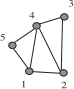
\includegraphics[width=0.25\linewidth]{images/spantreeexercise}
\end{lrbox}
\ifdefined\phAimage\else\newlength{\phAimage}\fi%
\setlength{\phAimage}{\ht\panelboxAimage+\dp\panelboxAimage}
\settototalheight{\phAimage}{\usebox{\panelboxAimage}}
\setlength{\panelmax}{\maxof{\panelmax}{\phAimage}}
\leavevmode%
% begin: side-by-side as tabular
% \tabcolsep change local to group
\setlength{\tabcolsep}{0\linewidth}
% @{} suppress \tabcolsep at extremes, so margins behave as intended
\par\medskip\noindent
\hspace*{0.375\linewidth}%
\begin{tabular}{@{}*{1}{c}@{}}
\begin{minipage}[c][\panelmax][t]{0.25\linewidth}\usebox{\panelboxAimage}\end{minipage}\tabularnewline
\parbox[t]{0.25\linewidth}{\captionof{figure}{A graph.\label{del-cont}}
}\end{tabular}\\
% end: side-by-side as tabular
}% end: group for a single side-by-side
\end{activity}
\begin{activity}[]\marginsymbol[-1em]{\pdftooltip{$\importantarrow$}{especially interesting}} \label{activity-245}
\leavevmode%
\begin{enumerate}[font=\bfseries,label=(\alph*),ref=\alph*]
\item\label{task-184} \marginsymbol[-2.5em]{} \hypertarget{p-1416}{}%
In how many ways may you properly color the vertices of a path on \(n\) vertices with \(x\) colors? Describe any dependence of the chromatic polynomial of a path on the number of vertices.%
\item\label{task-185} \marginsymbol[-2.5em]{} \hypertarget{p-1418}{}%
(Not tremendously hard.) In how many ways may you properly color the vertices of a cycle on \(n\) vertices with \(x\) colors? Describe any dependence of the chromatic polynomial of a cycle on the number of vertices.%
\end{enumerate}
\end{activity}
\begin{activity}[]\marginsymbol[-1em]{} \label{activity-246}
\hypertarget{p-1421}{}%
In how many ways may you properly color the vertices of a tree on \(n\) vertices with \(x\) colors?%
~{\tiny (h)}\end{activity}
\begin{activity}[]\marginsymbol[-1em]{\pdftooltip{$\importantarrow$}{especially interesting}} \label{activity-247}
\hypertarget{p-1425}{}%
What do you observe about the signs of the coefficients of the chromatic polynomial of the graph in \hyperref[del-cont]{Figure~\ref{del-cont}}? What about the signs of the coefficients of the chromatic polynomial of a path? Of a cycle? Of a tree? Make a conjecture about the signs of the coefficients of a chromatic polynomial and prove it.%
\end{activity}
\typeout{************************************************}
\typeout{Supplementary Problems 5.4 Supplementary Problems}
\typeout{************************************************}
\section[{Supplementary Problems}]{Supplementary Problems}\label{sec_inclexcl-suppprobs}
\begin{exerciselist}
\item[1.]\marginsymbol[-1em]{} \hypertarget{exercise-46}{}\hypertarget{p-1428}{}%
Each person attending a party has been asked to bring a prize. The person planning the party has arranged to give out exactly as many prizes as there are guests, but any person may win any number of prizes. If there are \(n\) guests, in how many ways may the prizes be given out so that nobody gets the prize that he or she brought?%
\par\smallskip
\item[2.]\marginsymbol[-1em]{} \hypertarget{exercise-47}{}\hypertarget{p-1430}{}%
There are \(m\) students attending a seminar in a room with \(n\) seats. The seminar is a long one, and in the middle the group takes a break. In how many ways may the students return to the room and sit down so that nobody is in the same seat as before?%
\par\smallskip
\item[3.]\marginsymbol[-1em]{} \hypertarget{exercise-48}{}\hypertarget{p-1432}{}%
What is the number of ways to pass out \(k\) pieces of candy from an unlimited supply of identical candy to \(n\) children (where \(n\) is fixed) so that each child gets between three and six pieces of candy (inclusive)? If you have done \hyperlink{candy-genfn}{Problem~1 of Supplementary Problems~\ref{sec_genfns-suppprobs}}, compare your answer in that problem with your answer in this one.%
\par\smallskip
\item[4.]\marginsymbol[-1em]{\pdftooltip{$\importantarrow$}{especially interesting}} \hypertarget{exercise-49}{}\hypertarget{p-1434}{}%
In how many ways may \(k\) distinct books be arranged on \(n\) shelves so that no shelf gets more than \(m\) books?%
\par\smallskip
\item[5.]\marginsymbol[-1em]{\pdftooltip{$\importantarrow$}{especially interesting}} \hypertarget{exercise-50}{}\hypertarget{p-1436}{}%
Suppose that \(n\) children join hands in a circle for a game at nursery school. The game involves everyone falling down (and letting go). In how many ways may they join hands in a circle again so that nobody is to the right of the same child that was previously to his or her right?%
\par\smallskip
\item[6.]\marginsymbol[-1em]{\pdftooltip{$\importantarrow$\ $*$}{especially interesting and difficult}} \hypertarget{Hora}{}\hypertarget{p-1438}{}%
Suppose that \(n\) people link arms in a folk-dance and dance in a circle. Later on they let go and dance some more, after which they link arms in a circle again. In how many ways can they link arms the second time so that no-one is next to a person with whom he or she linked arms before.%
\par\smallskip
\item[7.]\marginsymbol[-1em]{\pdftooltip{$\importantarrow$\ $*$}{especially interesting and difficult}} \hypertarget{exercise-52}{}\hypertarget{p-1444}{}%
(A challenge; the author has not tried to solve this one!) Redo \hyperlink{Hora}{Problem~6} in the case that there are \(n\) men and \(n\) women and when people arrange themselves in a circle they do so alternating gender.%
\par\smallskip
\item[8.]\marginsymbol[-1em]{\pdftooltip{$\importantarrow$}{especially interesting}} \hypertarget{exercise-53}{}\hypertarget{p-1445}{}%
Suppose we take two graphs \(G_1\) and \(G_2\) with disjoint vertex sets, we choose one vertex on each graph, and connect these two graphs by an edge \(e\) to get a graph \(G_{12}\). How does the chromatic polynomial of \(G_{12}\) relate to those of \(G_1\) and \(G_2\)?%
\par\smallskip
\end{exerciselist}
\typeout{************************************************}
\typeout{Chapter 6 Groups acting on sets}
\typeout{************************************************}
\chapter[{Groups acting on sets}]{Groups acting on sets}\label{groupsonsets}
\typeout{************************************************}
\typeout{Section 6.1 Permutation Groups}
\typeout{************************************************}
\section[{Permutation Groups}]{Permutation Groups}\label{sec_groups-permgroups}
\hypertarget{p-1448}{}%
Until now we have thought of permutations mostly as ways of listing the elements of a set. In this chapter we will find it very useful to think of permutations as functions. This will help us in using permutations to solve enumeration problems that cannot be solved by the quotient principle because they involve counting the blocks of a partition in which the blocks don't have the same size. We begin by studying the kinds of permutations that arise in situations where we have used the quotient principle in the past.%
\typeout{************************************************}
\typeout{Subsection 6.1.1 The rotations of a square}
\typeout{************************************************}
\subsection[{The rotations of a square}]{The rotations of a square}\label{subsection-58}
\leavevmode%
\begin{figure}
\centering
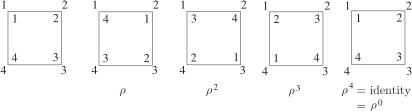
\includegraphics[width=0.95\linewidth]{images/RotationsOfSquare}
\caption{The four possible results of rotating a square and maintaining its position.\label{RotationsOfSquare}}
\end{figure}
\hypertarget{p-1449}{}%
In \hyperref[RotationsOfSquare]{Figure~\ref{RotationsOfSquare}} we show a square with its four vertices labelled 1, 2, 3, and 4. We have also labeled the spot in the plane where each of these vertices falls with the same label. Then we have shown the effect of rotating the square clockwise through 90, 180, 270, and 360 degrees (which is the same as rotating through 0 degrees). Underneath each of the rotated squares we have named the function that carries out the rotation. We use \(\rho\), the Greek letter pronounced ``row,'' to stand for a 90 degree clockwise rotation. We use \(\rho^2\) to stand for two 90 degree rotations, and so on. We can think of the function \(\rho\) as a function on the four element set\footnote{What we are doing is restricting the rotation \(\rho\) to the set \(\{1,2,3,4\}\).\label{fn-19}} \(\{1,2,3,4\}\). In particular, for any function \(\varphi\) (the Greek letter phi, usually pronounced ``fee,'' but sometimes ``fie'') from the plane back to itself that may move the square around but otherwise leaves it in the same place, we let \(\varphi(i)\) be the label of the place where vertex previously in position \(i\) is now. Thus \(\rho(1) =2\), \(\rho(2)=3\), \(\rho(3)=4\) and \(\rho(4) =1\). Notice that \(\rho\) is a permutation on the set \(\{1,2,3,4\}\).%
\begin{activity}[]\marginsymbol[-1em]{\pdftooltip{$\bullet$}{essential}} \label{composition1}
\hypertarget{p-1450}{}%
The composition\index{composition of functions}\index{functions!composition of} \(f\circ g\) of two functions \(f\) and \(g\) is defined by \(f\circ g(x) = f(g(x))\). Is \(\rho^3\) the composition of \(\rho\) and \(\rho^2\)? Does the answer depend on the order in which we write \(\rho\) and \(\rho^2\)? How is \(\rho^2\) related to \(\rho\)?%
\end{activity}
\begin{activity}[]\marginsymbol[-1em]{\pdftooltip{$\bullet$}{essential}} \label{activity-249}
\hypertarget{p-1452}{}%
Is the composition of two permutations always a permutation?%
\end{activity}
\hypertarget{p-1454}{}%
In \hyperref[composition1]{Problem~\ref{composition1}} you see that we can think of \(\rho^2\circ\rho\) as the result of first rotating by 90 degrees and then by another 180 degrees. In other words, the composition of two rotations is the same thing as first doing one and then doing the other. Of course there is nothing special about 90 degrees and 180 degrees.  As long as we first do one rotation through a multiple of 90 degrees and then another rotation through a multiple of 90 degrees, the composition of these rotations is a rotation through a multiple of 90 degrees.%
\par
\hypertarget{p-1455}{}%
If we first rotate by 90 degrees and then by 270 degrees then we have rotated by 360 degrees, which does nothing visible to the square. Thus we say that \(\rho^4\) is the ``identity function.'' In general the \terminology{identity function}\index{function!identity}\index{identity function} on a set \(S\), denoted by \(\iota\) (the Greek letter iota, pronounced eye-oh-ta) is the function that takes each element of the set to itself. In symbols, \(\iota(x) =x\) for every \(x\) in \(S\). Of course the identity function on a set is a permutation of that set.%
\typeout{************************************************}
\typeout{Subsection 6.1.2 Groups of Permutations}
\typeout{************************************************}
\subsection[{Groups of Permutations}]{Groups of Permutations}\label{subsection-59}
\begin{activity}[]\marginsymbol[-1em]{\pdftooltip{$\bullet$}{essential}} \label{activity-250}
\hypertarget{p-1456}{}%
For any function \(\varphi\) from a set \(S\) to itself, we define \(\varphi^n\) (for nonnegative integers \(n\)) inductively by \(\varphi^0 =
\iota\) and \(\varphi^n = \varphi^{n-1}\circ\varphi\) for every positive integer \(n\). If \(\varphi\) is a permutation, is \(\varphi^n\) a permutation? Based on your experience with previous inductive proofs, what do you expect \(\varphi^n\circ \varphi^m\) to be? What do you expect \((\varphi^m)^n\) to be? There is no need to prove these last two answers are correct, for you have, in effect, already done so in \hyperref[InductionRecursion]{Chapter~\ref{InductionRecursion}}.%
\end{activity}
\begin{activity}[]\marginsymbol[-1em]{\pdftooltip{$\bullet$}{essential}} \label{identityproperty}
\hypertarget{p-1458}{}%
If we perform the composition \(\iota\circ \varphi\) for any function \(\varphi\) from \(S\) to \(S\), what function do we get? What if we perform the composition \(\varphi\circ\iota\)?%
\end{activity}
\hypertarget{p-1460}{}%
What you have observed about iota in \hyperref[identityproperty]{Problem~\ref{identityproperty}} is called the \terminology{identity property}\index{identity property (for permutations)} of iota. In the context of permutations, people usually call the function \(\iota\) ``the identity'' rather than calling it ``iota.''%
\par
\hypertarget{p-1461}{}%
Since rotating first by 90 degrees and then by 270 degrees has the same effect as doing nothing, we can think of the 270 degree rotation as undoing what the 90 degree rotation does. For this reason we say that in the rotations of the square, \(\rho^3\) is the ``inverse'' of \(\rho\). In general, a function \(\varphi:T\rightarrow S\) is called an \terminology{inverse}\index{inverse function}\index{function!inverse} of a function \(\sigma:S
\rightarrow T\) (the lower case Greek letter sigma) if \(\varphi\circ \sigma= \sigma
\circ\varphi =
\iota\). For a slower introduction to inverses and practice with them, see \hyperref[digraphsoffunctions]{Section~\ref{digraphsoffunctions}} in \hyperref[Relations]{Appendix~\ref{Relations}}.  Since a permutation is a bijection, it has a unique inverse, as in \hyperref[digraphsoffunctions]{Section~\ref{digraphsoffunctions}}.  And since the inverse of a bijection is a bijection (again, as in the Appendix), the inverse of a permutation is a permutation.%
\par
\hypertarget{p-1462}{}%
We use \(\varphi^{-1}\) to denote the inverse of the permutation \(\varphi\). We've seen that the rotations of the square are functions that return the square to its original position but may move the vertices to different places. In this way we create permutations of the vertices of the square. We've observed three important properties of these permutations. \leavevmode%
\begin{itemize}[label=\textbullet]
\item{}\hypertarget{p-1463}{}%
(Identity Property)\index{identity property} These permutations include the identity permutation.%
\item{}\hypertarget{p-1464}{}%
(Inverse Property)\index{inverse property} Whenever these permutations include \(\varphi\), they also include \(\varphi^{-1}\).%
\item{}\hypertarget{p-1465}{}%
(Closure Property)\index{closure property}  Whenever these permutations include \(\varphi\) and \(\sigma\), they also include \(\varphi\circ\sigma\).%
\end{itemize}
%
\par
\hypertarget{p-1466}{}%
A set of permutations with these three properties is called a \terminology{permutation group}\footnote{The concept of a permutation group is a special case of the concept of a \terminology{group} that one studies in abstract algebra.  When we refer to a group in what follows, if you  know what groups are in the more abstract sense, you may use the word in this way. If you do not know about groups in this more abstract sense, then you may assume we mean permutation group when we say group.\label{fn-20}} or a group of permutations.\index{group of permutations}\index{permutation group} We call the group of permutations corresponding to rotations of the square the \terminology{rotation group}\index{rotation group} of the square. There is a similar rotation group with \(n\) elements for any regular \(n\)-gon.%
\begin{activity}[]\marginsymbol[-1em]{\pdftooltip{$\bullet$}{essential}} \label{activity-252}
\hypertarget{p-1467}{}%
If \(f:S\rightarrow T\), \(g:T\rightarrow X\), and \(h:X \rightarrow Y\), is \(h\circ(g\circ f) = (h\circ g)\circ f\)? What does this say about the status of the \emph{associative law}\index{associative law}%
\begin{equation*}
\rho\circ(\sigma\circ \varphi) = (\rho\circ \sigma)\circ\varphi
\end{equation*}
in a group of permutations?%
\end{activity}
\begin{activity}[]\marginsymbol[-1em]{\pdftooltip{$\bullet$}{essential}} \label{activity-253}
\leavevmode%
\begin{enumerate}[font=\bfseries,label=(\alph*),ref=\alph*]
\item\label{task-186} \marginsymbol[-2.5em]{} \hypertarget{p-1470}{}%
How should we define \(\varphi^{-n}\) for an element \(\varphi\) of a permutation group?%
~{\tiny (h)}\item\label{task-187} \marginsymbol[-2.5em]{} \hypertarget{p-1473}{}%
Will the two standard rules for exponents%
\begin{equation*}
a^ma^n=a^{m+n} \mbox{\ and\ }  (a^m)^n = a^{mn}
\end{equation*}
still hold if one or more of the exponents may be negative?%
\item\label{task-188} \marginsymbol[-2.5em]{} \hypertarget{p-1475}{}%
What would we have to prove to show that the rules still hold?%
\item\label{task-189} \marginsymbol[-2.5em]{} \hypertarget{p-1477}{}%
If the rules hold, give enough of the proof to show that you know how to do it; otherwise give a counterexample.%
\end{enumerate}
\end{activity}
\begin{activity}[]\marginsymbol[-1em]{\pdftooltip{$\bullet$}{essential}} \label{activity-254}
\hypertarget{p-1481}{}%
If a finite set of permutations satisfies the closure property is it a permutation group?%
~{\tiny (h)}\end{activity}
\begin{activity}[]\marginsymbol[-1em]{\pdftooltip{$\bullet$}{essential}} \label{dihedral1}
\hypertarget{p-1484}{}%
There are three dimensional geometric motions of the square that return it to its original position but move some of the vertices to other positions. For example, if we flip the square around a diagonal, most of it moves out of the plane during the flip, but the square ends up in the same place. Draw a figure like \hyperref[RotationsOfSquare]{Figure~\ref{RotationsOfSquare}} that shows all the possible results of such motions, including the ones shown in \hyperref[RotationsOfSquare]{Figure~\ref{RotationsOfSquare}}. Do the corresponding permutations form a group?%
\end{activity}
\begin{activity}[]\marginsymbol[-1em]{} \label{activity-256}
\hypertarget{p-1486}{}%
Let \(\sigma\) and \(\varphi\) be permutations.%
\begin{enumerate}[font=\bfseries,label=(\alph*),ref=\alph*]
\item\label{task-190} \marginsymbol[-2.5em]{} \hypertarget{p-1487}{}%
Why must \(\sigma\circ\varphi\) have an inverse?%
\item\label{task-191} \marginsymbol[-2.5em]{} \hypertarget{p-1489}{}%
Is \((\sigma\circ\varphi)^{-1}=\sigma^{-1}\varphi^{-1}\)? (Prove or give a counter-example.)%
~{\tiny (h)}\item\label{task-192} \marginsymbol[-2.5em]{} \hypertarget{p-1492}{}%
Is \((\sigma\circ\varphi)^{-1}= \varphi^{-1}\sigma^{-1}\)? (Prove or give a counter-example.)%
\end{enumerate}
\end{activity}
\begin{activity}[]\marginsymbol[-1em]{\pdftooltip{$\bullet$}{essential}} \label{activity-257}
\hypertarget{p-1494}{}%
Explain why the set of all permutations of four elements is a permutation group. How many elements does this group have? This group is called the \terminology{symmetric group on four letters}\index{symmetric group} and is denoted by \(S_4\).%
\end{activity}
\typeout{************************************************}
\typeout{Subsection 6.1.3 The symmetric group}
\typeout{************************************************}
\subsection[{The symmetric group}]{The symmetric group}\label{subsection-60}
\hypertarget{p-1496}{}%
In general, the set of all permutations of an \(n\)-element set is a group. It is called the \terminology{symmetric group on \(\mathbf n\) letters}\index{symmetric group}. We don't have nice geometric descriptions (like rotations) for all its elements, and it would be inconvenient to have to write down something like ``Let \(\sigma(1) =3\), \(\sigma(2) =1\), \(\sigma(3)=4\), and \(\sigma(4)=1\)'' each time we need to introduce a new permutation. We introduce a new notation for permutations that allows us to denote them \emph{reasonably} compactly and compose them reasonably quickly. If \(\sigma\) is the permutation of \(\{1,2,3,4\}\) given by \(\sigma(1)=3\), \(\sigma(2)=1\), \(\sigma(3) =4\) and \(\sigma(4) =2\), we write%
\begin{equation*}
\sigma =\left( \begin{matrix}1\amp 2\amp 3\amp 4\cr3\amp 1\amp 4\amp 2
\end{matrix} \right).
\end{equation*}
%
\par
\hypertarget{p-1497}{}%
We call this notation the \terminology{two row notation}\index{permutation!two row notation}\index{two row notation} for permutations. In the two row notation for a permutation of \(\{a_1,a_2,\ldots, a_n\}\), we write the numbers \(a_1\) through \(a_n\) in a one row and we write \(\sigma(a_1)\) through \(\sigma(a_n)\) in a row right below, enclosing both rows in parentheses. Notice that%
\begin{equation*}
\left( \begin{matrix}1\amp 2\amp 3\amp 4\cr3\amp 1\amp 4\amp 2
\end{matrix} \right) = \left(
\begin{matrix}2\amp 1\amp 4\amp 3\cr1\amp 3\amp 2\amp 4
\end{matrix} \right),
\end{equation*}
although the second ordering of the columns is rarely used.%
\par
\hypertarget{p-1498}{}%
If \(\varphi\) is given by%
\begin{equation*}
\varphi = \begin{pmatrix}1\amp 2\amp 3\amp 4\cr4\amp 1\amp 2\amp 3
\end{pmatrix} ,
\end{equation*}
then, by applying the definition of composition of functions, we may compute \(\sigma\circ
\varphi\) as shown in \hyperref[permutationproduct]{Figure~\ref{permutationproduct}}.%
\begin{figure}
\centering
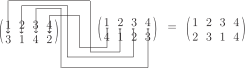
\includegraphics[width=0.73\linewidth]{images/productofpermutations}
\caption{How to multiply permutations in two-row notation.\label{permutationproduct}}
\end{figure}
\hypertarget{p-1499}{}%
We don't normally put the circle between two permutations in two row notation when we are composing them, and refer to the operation as multiplying the permutations, or as the product of the permutations. To see how \hyperref[permutationproduct]{Figure~\ref{permutationproduct}} illustrates composition, notice that the arrow starting at 1 in \(\varphi\) goes to 4. Then from the 4 in \(\varphi\) it goes to the 4 in \(\sigma\) and then to 2. This illustrates that \(\varphi(1)=4\) and \(\sigma(4) =2\), so that \(\sigma(\varphi(1))=2\).%
\begin{activity}[]\marginsymbol[-1em]{} \label{activity-258}
\hypertarget{p-1500}{}%
For practice, compute \(\begin{pmatrix}1\amp 2\amp 3\amp 4\amp 5\cr3\amp 4\amp 1\amp 5\amp 2
\end{pmatrix}
\begin{pmatrix}1\amp 2\amp 3\amp 4\amp 5\cr 4\amp 3\amp 5\amp 1\amp 2
\end{pmatrix}\).%
\end{activity}
\typeout{************************************************}
\typeout{Subsection 6.1.4 The dihedral group}
\typeout{************************************************}
\subsection[{The dihedral group}]{The dihedral group}\label{subsection-61}
\index{dihedral group}\hypertarget{p-1502}{}%
We found four permutations that correspond to rotations of the square. In \hyperref[dihedral1]{Problem~\ref{dihedral1}} you found four permutations that correspond to flips of the square in space. One flip fixes the vertices in the places labeled 1 and 3 and interchanges the vertices in the places labeled 2 and 4. Let us denote it by \(\varphi_{1|3}\). One flip fixes the vertices in the positions labeled 2 and 4 and interchanges those in the positions labeled 1 and 3. Let us denote it by \(\varphi{2|4}\). One flip interchanges the vertices in the places labeled 1 and 2 and also interchanges those in the places labeled 3 and 4. Let us denote it by \(\varphi_{12|34}\). The fourth flip interchanges the vertices in the places labeled 1 and 4 and interchanges those in the places labeled 2 and 3. Let us denote it by \(\varphi_{14|23}\). Notice that \(\varphi_{1|3}\) is a permutation that takes the vertex in place 1 to the vertex in place 1 and the vertex in place 3 to the vertex in place 3, while \(\varphi_{12|34}\) is a permutation that takes the edge between places 1 and 2 to the edge between places 2 and 1 (which is the same edge) and takes the edge between places 3 and 4 to the edge between places 4 and 3 (which is the same edge). This should help to explain the similarity in the notation for the two different kinds of flips.%
\begin{activity}[]\marginsymbol[-1em]{\pdftooltip{$\bullet$}{essential}} \label{dihedral2}
\hypertarget{p-1503}{}%
Write down the two-row notation for \(\rho^3\), \(\varphi_{2|4}\), \(\varphi_{12|34}\) and \(\varphi_{2|4}\circ \varphi_{12|34}\). Remember that \(\sigma(i)\) stands for the position where the vertex that originated in position \(i\) is after we apply \(\sigma\).%
\end{activity}
\begin{activity}[]\marginsymbol[-1em]{} \label{activity-260}
\hypertarget{p-1505}{}%
(You may have already done this problem in \hyperref[dihedral1]{Problem~\ref{dihedral1}}, in which case you need not do it again!) In \hyperref[dihedral1]{Problem~\ref{dihedral1}}, if a rigid motion of three-dimensional space returns the square to its original position, in how many places can vertex number one land? Once the location of vertex number one is decided, how many possible locations are there for vertex two? Once the locations of vertex one and vertex two are decided, how many locations are there for vertex three? Answer the same question for vertex four. What does this say about the relationship between the four rotations and four flips described above and the permutations you described in \hyperref[dihedral1]{Problem~\ref{dihedral1}}?%
\end{activity}
\hypertarget{p-1507}{}%
The four rotations and four flips of the square described before \hyperref[dihedral2]{Problem~\ref{dihedral2}} form a group called the dihedral group of the square. Sometimes the group is denoted \(D_8\) because it has eight elements, and sometimes the group is denoted by \(D_4\) because it deals with four vertices! Let us agree to use the notation \(D_4\) for the dihedral group of the square. There is a similar dihedral group, denoted by \(D_{n}\), of all the rigid motions of three-dimensional space that return a regular \(n\)-gon to its original position (but might put the vertices in different places.)%
\begin{activity}[]\marginsymbol[-1em]{} \label{activity-261}
\hypertarget{p-1508}{}%
Another view of the dihedral group of the square is that it is the group of all distance preserving functions, also called \terminology{isometries}, \index{isometry} from a square to itself.  Notice that an isometry must be a bijection.  Any rigid motion of the square preserves the distances between all points of the square.  However, it is conceivable that there might be some isometries that do not arise from rigid motions.  (We will see some later on in the case of a cube.)  Show that there are exactly eight isometires (distance preserving functions) from a square to itself.%
~{\tiny (h)}\end{activity}
\begin{activity}[]\marginsymbol[-1em]{} \label{activity-262}
\hypertarget{p-1511}{}%
How many elements does the group \(D_n\) have? Prove that you are correct.%
\end{activity}
\begin{activity}[]\marginsymbol[-1em]{} \label{cube1-prob}
\hypertarget{p-1513}{}%
In \hyperref[cube1]{Figure~\ref{cube1}} we show a cube with the positions of its vertices and faces labeled.  As with motions of the square, we let \(\varphi(x)\) be the label of the place where vertex previously in position \(x\) is now.%
\begin{figure}
\centering
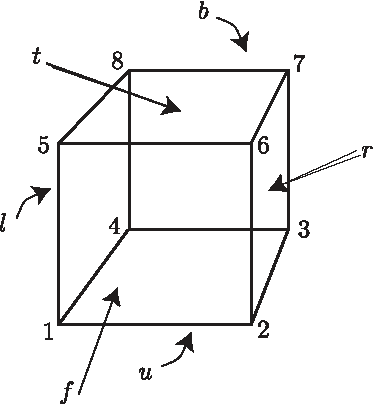
\includegraphics[width=0.5\linewidth]{images/cube1}
\caption{A cube with the positions of its vertices and faces labelled.  The curved arrows point to the positions that are blocked by the cube.\label{cube1}}
\end{figure}
\begin{enumerate}[font=\bfseries,label=(\alph*),ref=\alph*]
\item\label{task-193} \marginsymbol[-2.5em]{} \hypertarget{p-1514}{}%
Write in two row notation the permutation \(\rho\) of the vertices that corresponds to rotating the cube 90 degrees around a vertical axis through the faces \(t\) (for top) and \(u\) (for underneath). (Rotate in a right-handed fashion around this axis, meaning that vertex 6 goes to the back and vertex 8 comes to the front.)%
\item\label{task-194} \marginsymbol[-2.5em]{} \hypertarget{p-1516}{}%
Write in two row notation the permutation \(\varphi\) that rotates the cube 120 degrees around the diagonal from vertex 1 to vertex 7 and carries vertex 8 to vertex 6.%
\item\label{task-195} \marginsymbol[-2.5em]{} \hypertarget{p-1518}{}%
Compute the two row notation for \(\rho \circ \varphi\)%
\item\label{task-196} \marginsymbol[-2.5em]{} \hypertarget{p-1520}{}%
Is the permutation \(\rho\circ\varphi\) a rotation of the cube around some axis?  If so, say what the axis is and how many degrees we rotate around the axis.  If \(\rho\circ\varphi\) is not a rotation, give a geometic description of it.%
\end{enumerate}
\end{activity}
\begin{activity}[]\marginsymbol[-1em]{\pdftooltip{$\importantarrow$\ {\Large$\cdot$}}{especially interesting and essential for this or the next section}} \label{activity-264}
\hypertarget{p-1522}{}%
How many permutations are in the group \(R\)? \(R\) is sometimes called the ``rotation group'' of the cube. Can you justify this?%
~{\tiny (h)}\end{activity}
\begin{activity}[]\marginsymbol[-1em]{} \label{activity-265}
\hypertarget{p-1525}{}%
As with a two-dimensional figure, it is possible to talk about isometries of a three-dimensional figure. These are distance preserving functions from the figure to itself. The function that reflects the cube in \hyperref[cube1]{Figure~\ref{cube1}} through a plane halfway between the bottom face and top face exchanges the vertices 1 and 5, 2 and 6, 3 and 7, and 4 and 8 of the cube. This function preserves distances between points in the cube. However, it cannot be achieved by a rigid motion of the cube because a rigid motion that takes vertex 1 to vertex 5, vertex 2 to vertex 6, vertex 3 to vertex 7, and vertex 4 to vertex 8 would not return the cube to its original location; rather it would put the bottom of the cube where its top previously was and would put the rest of the cube above that square rather than below it.%
\begin{enumerate}[font=\bfseries,label=(\alph*),ref=\alph*]
\item\label{task-197} \marginsymbol[-2.5em]{} \hypertarget{p-1526}{}%
How many elements are there in the group of permutations of \([8]\)   that correspond to isometries of the cube?%
~{\tiny (h)}\item\label{task-198} \marginsymbol[-2.5em]{} \hypertarget{p-1529}{}%
Is every permutation of \([8]\) that corresponds to an isometry either a rotation or a reflection?%
~{\tiny (h)}\end{enumerate}
\end{activity}
\typeout{************************************************}
\typeout{Subsection 6.1.5 Group tables (Optional)}
\typeout{************************************************}
\subsection[{Group tables (Optional)}]{Group tables (Optional)}\label{subsection-62}
\hypertarget{p-1532}{}%
We can always figure out the composition of two permutations of the same set by using the definition of composition, but if we are going to work with a given permutation group again and again, it is worth making the computations once and recording them in a table. For example the group of rotations of the square may be represented as in \hyperref[rotationgrouptable]{Table~\ref{rotationgrouptable}}. We list the elements of our group, with the identity first, across the top of the table and down the left side of the table, using the same order both times. Then in the row labeled by the group element \(\sigma\) and the column labelled by the group element \(\varphi\), we write the composition \(\sigma\circ \varphi\), expressed in terms of the elements we have listed on the top and on the left side. Since a group of permutations is closed under composition, the result \(\sigma\circ \varphi\) will always be expressible as one of these elements.%
\begin{table}
\centering
\begin{tabular}{lAllll}
\(\circ\)&\(\iota\)&\(\rho\)&\(\rho^2\)&\(\rho^3\)\tabularnewline\hrulethin
\(\iota\)&\(\iota\)&\(\rho\)&\(\rho^2\)&\(\rho^3\)\tabularnewline[0pt]
\(\rho\)&\(\rho\)&\(\rho^2\)&\(\rho^3\)&\(\iota\)\tabularnewline[0pt]
\(\rho^2\)&\(\rho^2\)&\(\rho^3\)&\(\iota\)&\(\rho\)\tabularnewline[0pt]
\(\rho^3\)&\(\rho^3\)&\(\iota\)&\(\rho\)&\(\rho^2\)
\end{tabular}
\caption{The group table for the rotations of a square.\label{rotationgrouptable}}
\end{table}
\begin{activity}[]\marginsymbol[-1em]{} \label{activity-266}
\hypertarget{p-1533}{}%
In \hyperref[rotationgrouptable]{Table~\ref{rotationgrouptable}}, all the entries in a row (not including the first entry, the one to the left of the line) are different. Will this be true in any group table for a permutation group? Why or why not? Also in \hyperref[rotationgrouptable]{Table~\ref{rotationgrouptable}} all the entries in a column (not including the first entry, the one above the line) are different. Will this be true in any group table for a permutation group? Why or why not?%
\end{activity}
\begin{activity}[]\marginsymbol[-1em]{} \label{activity-267}
\hypertarget{p-1535}{}%
In \hyperref[rotationgrouptable]{Table~\ref{rotationgrouptable}}, every element of the group appears in every row (even if you don't include the first element, the one before the line). Will this be true in any group table for a permutation group? Why or why not? Also in \hyperref[rotationgrouptable]{Table~\ref{rotationgrouptable}} every element of the group appears in every column (even if you don't include the first entry, the one before the line). Will this be true in any group table for a permutation group? Why or why not?%
\end{activity}
\begin{activity}[]\marginsymbol[-1em]{\pdftooltip{$\bullet$}{essential}} \label{dihedral3}
\hypertarget{p-1537}{}%
Write down the group table for the dihedral group \(D_4\). Use the \(\varphi\) notation described above to denote the flips. (Hints: Part of the table has already been written down. Will you need to think hard to write down the last row? Will you need to think hard to write down the last column? When you multiply a product like \(\varphi_{1|3}
\circ \rho\) remember that we defined \(\varphi_{1|3}\) to be the flip that fixes the vertex in position 1 and the vertex in position 3, \emph{not} the one that fixes the vertex on the square labelled 1 and the vertex on the square labelled 3.)%
\end{activity}
\hypertarget{p-1538}{}%
You may notice that the associative law, the identity property, and the inverse property are three of the most important rules that we use in regrouping parentheses in algebraic expressions when solving equations. There is one property we have not yet mentioned, the \terminology{commutative law}\index{commutative law} which would say that \(\sigma\circ \varphi =
\varphi\circ\sigma\). It is easy to see from the group table of \(R_4\) that it satisfies the commutative law.%
\begin{activity}[]\marginsymbol[-1em]{} \label{activity-269}
\hypertarget{p-1539}{}%
Does the commutative law hold in all permutation groups?%
\end{activity}
\typeout{************************************************}
\typeout{Subsection 6.1.6 Subgroups}
\typeout{************************************************}
\subsection[{Subgroups}]{Subgroups}\label{subsection-63}
\hypertarget{p-1541}{}%
We have seen that the dihedral group \(D_4\) contains a copy of the group of rotations of the square. When one group \(G\) of permutations of a set \(S\) is a subset of another group \(G'\) of permutations of \(S\), we say that \(G\) is a \terminology{subgroup}\index{subgroup} of \(G'\). %
\begin{activity}[]\marginsymbol[-1em]{\pdftooltip{$\bullet$}{essential}} \label{S4}
\hypertarget{p-1542}{}%
Find all subgroups of the group \(D_4\).%
~{\tiny (h)}\end{activity}
\begin{activity}[]\marginsymbol[-1em]{} \label{activity-271}
\hypertarget{p-1545}{}%
Can you find subgroups of the symmetric group \(S_4\) with two elements? Three elements? Four elements? Six elements? (For each positive answer, describe a subgroup. For each negative answer, explain why not.)%
\end{activity}
\typeout{************************************************}
\typeout{Subsection 6.1.7 The cycle structure of a permutation}
\typeout{************************************************}
\subsection[{The cycle structure of a permutation}]{The cycle structure of a permutation}\label{subsection-64}
\hypertarget{p-1547}{}%
There is an even more efficient way to write down permutations. Notice that the product in \hyperref[permutationproduct]{Figure~\ref{permutationproduct}} is \(\begin{pmatrix}1\amp 2\amp 3\amp 4\cr2\amp 3\amp 1\amp 4
\end{pmatrix}\). We have drawn the directed graph of this permutation in \hyperref[permutationcycledigraph]{Figure~\ref{permutationcycledigraph}}.%
\begin{figure}
\centering
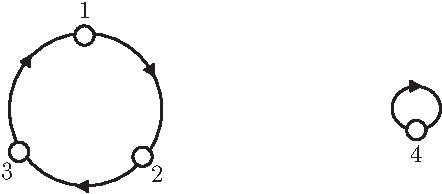
\includegraphics[width=0.73\linewidth]{images/permutationcycledigraph}
\caption{The directed graph of a permutation .\label{permutationcycledigraph}}
\end{figure}
\hypertarget{p-1548}{}%
You see that the graph has two directed cycles, the rather trivial one with vertex 4 pointing to itself, and the nontrivial one with vertex 1 pointing to vertex 2 pointing to vertex 3 which points back to vertex 1. A permutation is called a \terminology{cycle}\index{cycle (of a permutation)}\index{permutation!cycle of} if its digraph consists of exactly one cycle. Thus \(\begin{pmatrix}1\amp 2\amp 3\cr2\amp 3\amp 1
\end{pmatrix}\) is a cycle but \(\begin{pmatrix}1\amp 2\amp 3\amp 4\cr2\amp 3\amp 1\amp 4
\end{pmatrix}\) is not a cycle by our definition. We write \((1\ 2\ 3)\) or \((2\ 3\ 1)\) or \((3\ 1\ 2)\) to stand for the cycle \(\sigma =\begin{pmatrix}1\amp 2\amp 3\cr2\amp 3\amp 1
\end{pmatrix}\).%
\par
\hypertarget{p-1549}{}%
We can describe cycles in another way as well. A \terminology{cycle} of the permutation \(\sigma\) is a list \((i\
\sigma(i)\
\sigma^2(i)
\ \ldots\
\sigma^n(i))\) that does not have repeated elements while the list \((i\ \sigma(i)\
\sigma^2(i)\ \ldots\ \sigma^n(i))\ \sigma^{n+1}(i))\) does have repeated elements.%
\begin{activity}[]\marginsymbol[-1em]{} \label{activity-272}
\hypertarget{p-1550}{}%
If the list \((i\ \sigma(i)\ \sigma^2(i)\ \ldots\ \sigma^n(i))\) does not have repeated elements but the list \((i\ \sigma(i)\ \sigma^2(i)\ \ldots\ \sigma^n(i)\ \sigma^{n+1}(i))\) does have repeated elements, then what is \(\sigma^{n+1}(i)\)?%
~{\tiny (h)}\end{activity}
\hypertarget{p-1553}{}%
We say \(\sigma^j(i)\) is an \terminology{element} \index{cycle (of a permutation)!element of}of the cycle \((i\ \sigma(i)\ \sigma^2(i)\ \ldots\ \sigma^n(i))\).  Notice that the case \(j=0\) means \(i\) is an element of the cycle.  Notice also that if \(j\gt n\), \(\sigma^j(i) = \sigma^{j-n-1}(i)\), so the distinct elements of the cycle are \(i\), \(\sigma(i)\), \(\sigma^2(i)\), through \(\sigma^n(i)\). We think of the cycle \((i\ \sigma(i)\ \sigma^2(i)\ \ldots\ \sigma^n(i))\) as representing the permutation \(\sigma\) restricted to the set of elements of the cycle. We say that the cycles \((i\
\sigma(i)\
\sigma^2(i)\ \ldots\ \sigma^n(i))\) and \((j\
\sigma(j)\
\sigma^2(j)\ \ldots\ \sigma^n(j))\) are \terminology{equivalent} \index{cycle (of a permutation)!equivalent}\index{equivalent cycle}if there is an integer \(k\) such that \(j=
\sigma^k(i)\).%
\begin{activity}[]\marginsymbol[-1em]{\pdftooltip{$\bullet$}{essential}} \label{d4-cycles}
\hypertarget{p-1554}{}%
Find the cycles of the permutations \(\rho\), \(\varphi_{1|3}\) and \(\varphi_{12|34}\) in the group \(D_4\).%
\end{activity}
\begin{activity}[]\marginsymbol[-1em]{} \label{permutation-cycles}
\hypertarget{p-1556}{}%
Find the cycles of the permutation%
\begin{equation*}
\begin{pmatrix}1\amp 2\amp 3\amp 4\amp 5\amp 6\amp 7\amp 8\amp 9\cr
3\amp 4\amp 6\amp 2\amp 9\amp 7\amp 1\amp 5\amp 8
\end{pmatrix}\text{.}
\end{equation*}
%
\end{activity}
\begin{activity}[]\marginsymbol[-1em]{} \label{common-elements}
\hypertarget{p-1558}{}%
If two cycles of \(\sigma\) have an element in common, what can we say about them?%
\end{activity}
\hypertarget{p-1560}{}%
\hyperref[common-elements]{Problem~\ref{common-elements}} leads almost immediately to the following theorem.%
\begin{theorem}[{}]\label{unique-partition}
\hypertarget{p-1561}{}%
for each permutation \(\sigma\) of a set \(S\), there is a unique partition of \(S\) each of whose blocks is the set of elements of a cycle of \(\sigma\).%
\end{theorem}
\hypertarget{p-1562}{}%
More informally, we may say that every permutation partitions its domain into disjoint cycles. We call the set of cycles of a permutation the \terminology{cycle decomposition} of the permutation. Since the cycles of a permutation \(\sigma\) tell us \(\sigma(x)\) for every \(x\) in the domain of \(\sigma\), the cycle decomposition of a permutation completely determines the permutation. Using our informal language, we can express this idea in the following corollary to \hyperref[unique-partition]{Theorem~\ref{unique-partition}}.%
\begin{corollary}[{}]\label{corollary-2}
\hypertarget{p-1563}{}%
Every partition of a set \(S\) into cycles determins a unique permutation of \(S\).%
\end{corollary}
\begin{activity}[]\marginsymbol[-1em]{} \label{activity-276}
\hypertarget{p-1564}{}%
Prove \hyperref[unique-partition]{Theorem~\ref{unique-partition}}.%
\end{activity}
\hypertarget{p-1566}{}%
In \hyperref[d4-cycles]{Problems~\ref{d4-cycles}} and \hyperref[permutation-cycles]{Problem~\ref{permutation-cycles}} you found the cycle decomposition of typical elements of the group \(D_4\) and of the permutation%
\begin{equation*}
\begin{pmatrix}1\amp 2\amp 3\amp 4\amp 5\amp 6\amp 7\amp 8\amp 9\cr
3\amp 4\amp 6\amp 2\amp 9\amp 7\amp 1\amp 5\amp 8
\end{pmatrix}
\end{equation*}
%
\par
\hypertarget{p-1567}{}%
The group of all rotations of the square is simply the set of the four powers of the cycle \(\rho = (1\ 2\ 3\ 4)\).  for this reason it is called a \terminology{cyclic group}\footnote{The phrace cyclic group applies in a more general (but similar) situation.  Namely the set of all powers of any member of a group is called a cyclic group.\label{fn-21}}\index{cyclic group} and is often denoted by \(C_4\).  Similarly, the rotation group of an \(n\)-gon is usually denoted \(C_n\).%
\begin{activity}[]\marginsymbol[-1em]{\pdftooltip{$\importantarrow$}{especially interesting}} \label{activity-277}
\hypertarget{p-1568}{}%
Write a recurrence for the number \(c(k,n)\) for the number of permutations of \([k]\) that have exactly \(n\) cycles, including 1-cycles. Use it to write a table of \(c(k,n)\) for \(k\) between 1 and 7 inclusive. Can you find a relationship between \(c(k,n)\) and any of the other families of special numbers such as binomial coefficients, Stirling numbers, Lah numbers, etc. we have studied? If you find such a relationship, prove you are right.%
~{\tiny (h)}\end{activity}
\begin{activity}[]\marginsymbol[-1em]{\pdftooltip{$\importantarrow$\ {\Large$\cdot$}}{especially interesting and essential for this or the next section}} \label{activity-278}
\hypertarget{p-1573}{}%
(Relevant to \hyperref[expogenfun]{Appendix~\ref{expogenfun}}.) A permutation \(\sigma\) is called an \terminology{involution}\index{involution} if \(\sigma^2=\iota\). When you write an involution as a product of disjoint cycles, what is special about the cycles?%
\end{activity}
\typeout{************************************************}
\typeout{Section 6.2 Groups Acting on Sets}
\typeout{************************************************}
\section[{Groups Acting on Sets}]{Groups Acting on Sets}\label{sec_groups-groupsact}
\hypertarget{p-1575}{}%
We defined the rotation group \(R_4\) and the dihedral group \(D_4\) as groups of permutations of the vertices of a square. These permutations represent rigid motions of the square in the plane and in three dimensional space respectively. The square has geometric features of interest other than its vertices; for example its diagonals, or its edges. Any geometric motion of the square that returns it to its original position takes each diagonal to a possibly different diagonal, and takes each edge to a possibly different edge. In \hyperref[rotate-square]{Figure~\ref{rotate-square}} we show the results on the sides and diagonals of the rotations of a square. The rotation group permutes the sides of the square and permutes the diagonals of the square as it rotates the square. Thus, we say the rotation group ``acts'' on the sides and diagonals of the square.%
\begin{figure}
\centering
% group protects changes to lengths, releases boxes (?)
{% begin: group for a single side-by-side
% set panel max height to practical minimum, created in preamble
\setlength{\panelmax}{0pt}
\ifdefined\panelboxAimage\else\newsavebox{\panelboxAimage}\fi%
\begin{lrbox}{\panelboxAimage}
\resizebox{0.19\linewidth}{!}{{
\begin{tikzpicture}
\draw (0,0) --(0,2) -- (2,2) -- (2,0) -- (0,0);
\draw (0,0) -- (2,2);
\draw (2,0) -- (0,2);
\node [above left] at (0,2) {1};
\node [above right] at (2,2) {2};
\node [below right] at (2,0) {3};
\node [below left] at (0,0) {4};
\node [above] at (0.8,1.35) {$d_{13}$};
\node [above] at (0.8,0.15) {$d_{24}$};
\node [left] at (0,1) {$s_4$};
\node [below] at (1,0) {$s_3$};
\node [right] at (2,1) {$s_2$};
\node [above] at (1,2) {$s_1$};
\end{tikzpicture}
}
}\end{lrbox}
\ifdefined\phAimage\else\newlength{\phAimage}\fi%
\setlength{\phAimage}{\ht\panelboxAimage+\dp\panelboxAimage}
\settototalheight{\phAimage}{\usebox{\panelboxAimage}}
\setlength{\panelmax}{\maxof{\panelmax}{\phAimage}}
\ifdefined\panelboxBimage\else\newsavebox{\panelboxBimage}\fi%
\begin{lrbox}{\panelboxBimage}
\resizebox{0.19\linewidth}{!}{{
\begin{tikzpicture}
\draw (0,0) --(0,2) -- (2,2) -- (2,0) -- (0,0);
\draw (0,0) -- (2,2);
\draw (2,0) -- (0,2);
\node [above left] at (0,2) {1};
\node [above right] at (2,2) {2};
\node [below right] at (2,0) {3};
\node [below left] at (0,0) {4};
\node [above] at (0.8,1.35) {$d_{24}$};
\node [above] at (0.8,0.15) {$d_{13}$};
\node [left] at (0,1) {$s_3$};
\node [below] at (1,0) {$s_2$};
\node [right] at (2,1) {$s_1$};
\node [above] at (1,2) {$s_4$};
\node [below] at (1,-0.5) {$\rho$};
\end{tikzpicture}
}
}\end{lrbox}
\ifdefined\phBimage\else\newlength{\phBimage}\fi%
\setlength{\phBimage}{\ht\panelboxBimage+\dp\panelboxBimage}
\settototalheight{\phBimage}{\usebox{\panelboxBimage}}
\setlength{\panelmax}{\maxof{\panelmax}{\phBimage}}
\ifdefined\panelboxCimage\else\newsavebox{\panelboxCimage}\fi%
\begin{lrbox}{\panelboxCimage}
\resizebox{0.19\linewidth}{!}{{
\begin{tikzpicture}
\draw (0,0) --(0,2) -- (2,2) -- (2,0) -- (0,0);
\draw (0,0) -- (2,2);
\draw (2,0) -- (0,2);
\node [above left] at (0,2) {1};
\node [above right] at (2,2) {2};
\node [below right] at (2,0) {3};
\node [below left] at (0,0) {4};
\node [above] at (0.8,1.35) {$d_{13}$};
\node [above] at (0.8,0.15) {$d_{24}$};
\node [left] at (0,1) {$s_2$};
\node [below] at (1,0) {$s_1$};
\node [right] at (2,1) {$s_4$};
\node [above] at (1,2) {$s_3$};
\node [below] at (1,-0.5) {$\rho^2$};
\end{tikzpicture}
}
}\end{lrbox}
\ifdefined\phCimage\else\newlength{\phCimage}\fi%
\setlength{\phCimage}{\ht\panelboxCimage+\dp\panelboxCimage}
\settototalheight{\phCimage}{\usebox{\panelboxCimage}}
\setlength{\panelmax}{\maxof{\panelmax}{\phCimage}}
\ifdefined\panelboxDimage\else\newsavebox{\panelboxDimage}\fi%
\begin{lrbox}{\panelboxDimage}
\resizebox{0.19\linewidth}{!}{{
\begin{tikzpicture}
\draw (0,0) --(0,2) -- (2,2) -- (2,0) -- (0,0);
\draw (0,0) -- (2,2);
\draw (2,0) -- (0,2);
\node [above left] at (0,2) {1};
\node [above right] at (2,2) {2};
\node [below right] at (2,0) {3};
\node [below left] at (0,0) {4};
\node [above] at (0.8,1.35) {$d_{24}$};
\node [above] at (0.8,0.15) {$d_{13}$};
\node [left] at (0,1) {$s_1$};
\node [below] at (1,0) {$s_4$};
\node [right] at (2,1) {$s_3$};
\node [above] at (1,2) {$s_2$};
\node [below] at (1,-0.5) {$\rho^3$};
\end{tikzpicture}
}
}\end{lrbox}
\ifdefined\phDimage\else\newlength{\phDimage}\fi%
\setlength{\phDimage}{\ht\panelboxDimage+\dp\panelboxDimage}
\settototalheight{\phDimage}{\usebox{\panelboxDimage}}
\setlength{\panelmax}{\maxof{\panelmax}{\phDimage}}
\ifdefined\panelboxEimage\else\newsavebox{\panelboxEimage}\fi%
\begin{lrbox}{\panelboxEimage}
\resizebox{0.19\linewidth}{!}{{
\begin{tikzpicture}
\draw (0,0) --(0,2) -- (2,2) -- (2,0) -- (0,0);
\draw (0,0) -- (2,2);
\draw (2,0) -- (0,2);
\node [above left] at (0,2) {1};
\node [above right] at (2,2) {2};
\node [below right] at (2,0) {3};
\node [below left] at (0,0) {4};
\node [above] at (0.8,1.35) {$d_{13}$};
\node [above] at (0.8,0.15) {$d_{24}$};
\node [left] at (0,1) {$s_4$};
\node [below] at (1,0) {$s_3$};
\node [right] at (2,1) {$s_2$};
\node [above] at (1,2) {$s_1$};
\node [below] at (1,-0.5) {$\begin{aligned}\rho^4 &=\text{identity}\\&=\rho^0\end{aligned}$};
\end{tikzpicture}
}
}\end{lrbox}
\ifdefined\phEimage\else\newlength{\phEimage}\fi%
\setlength{\phEimage}{\ht\panelboxEimage+\dp\panelboxEimage}
\settototalheight{\phEimage}{\usebox{\panelboxEimage}}
\setlength{\panelmax}{\maxof{\panelmax}{\phEimage}}
\leavevmode%
% begin: side-by-side as tabular
% \tabcolsep change local to group
\setlength{\tabcolsep}{0.005\linewidth}
% @{} suppress \tabcolsep at extremes, so margins behave as intended
\par\medskip\noindent
\hspace*{0.005\linewidth}%
\begin{tabular}{@{}*{5}{c}@{}}
\begin{minipage}[c][\panelmax][t]{0.19\linewidth}\usebox{\panelboxAimage}\end{minipage}&
\begin{minipage}[c][\panelmax][t]{0.19\linewidth}\usebox{\panelboxBimage}\end{minipage}&
\begin{minipage}[c][\panelmax][t]{0.19\linewidth}\usebox{\panelboxCimage}\end{minipage}&
\begin{minipage}[c][\panelmax][t]{0.19\linewidth}\usebox{\panelboxDimage}\end{minipage}&
\begin{minipage}[c][\panelmax][t]{0.19\linewidth}\usebox{\panelboxEimage}\end{minipage}\end{tabular}\\
% end: side-by-side as tabular
}% end: group for a single side-by-side
\caption{The results on the sides and diagonals of rotating the square\label{rotate-square}}
\end{figure}
\begin{activity}[]\marginsymbol[-1em]{} \label{activity-279}
\leavevmode%
\begin{enumerate}[font=\bfseries,label=(\alph*),ref=\alph*]
\item\label{task-199} \marginsymbol[-2.5em]{} \hypertarget{p-1576}{}%
Write down the two-line notation for the permutation \(\overline{\rho}\) that a \(90\) degree rotation does to the sides of the square.%
\item\label{task-200} \marginsymbol[-2.5em]{} \hypertarget{p-1578}{}%
Write down the two-line notation for the permutation \(\overline{\rho^2}\) that  a 180 degree rotation does to the sides of the square.%
\item\label{task-201} \marginsymbol[-2.5em]{} \hypertarget{p-1580}{}%
Is \(\overline{\rho^2} = \overline\rho\circ\overline\rho\)? Why or why not?%
\item\label{task-202} \marginsymbol[-2.5em]{} \hypertarget{p-1582}{}%
Write down the two-line notation for the permutation \(\widehat{\rho}\) that a 90 degree rotation does to the diagonals \(d_{13}\) and \(d_{24}\) of the square.%
\item\label{task-203} \marginsymbol[-2.5em]{} \hypertarget{p-1584}{}%
Write down the two-line notation for the permutation \(\widehat{\rho^2}\) that a 180 degree rotation does to the diagonals \(d_{13}\) and \(d_{24}\) of the square.%
\item\label{task-204} \marginsymbol[-2.5em]{} \hypertarget{p-1586}{}%
Is \(\widehat{\rho^2} = \widehat{\rho}\circ\widehat{\rho}\)? Why or why not? What familiar permutation is \(\widehat{\rho^2}\) in this case?%
\end{enumerate}
\end{activity}
\hypertarget{p-1588}{}%
We have seen that the fact that we have defined a permutation group as the permutations of some specific set doesn't preclude us from thinking of the elements of that group as permuting the elements of some other set as well. In order to keep track of which permutations of which set we are using to define our group and which other set is being permuted as well, we introduce some new language and notation. We are going to say that the group \(D_4\) ``acts'' on the edges and diagonals of a square and the group \(R\) of permutations of the vertices of a cube that arise from rigid motions of the cube ``acts'' on the edges, faces, diagonals, etc. of the cube.%
\begin{activity}[]\marginsymbol[-1em]{\pdftooltip{$\bullet$}{essential}} \label{activity-280}
\hypertarget{p-1589}{}%
In \hyperref[cube1]{Figure~\ref{cube1}} we show a cube with the positions of its vertices and faces labeled. As with motions of the square, we let we let \(\varphi(x)\) be the label of the place where vertex previously in position \(x\) is now.%
\begin{enumerate}[font=\bfseries,label=(\alph*),ref=\alph*]
\item\label{actsonparta} \marginsymbol[-2.5em]{} \hypertarget{p-1590}{}%
In \hyperref[cube1-prob]{Problem~\ref{cube1-prob}} we wrote in two row notation the permutation \(\rho\) of the vertices that corresponds to rotating the cube 90 degrees around a vertical axis through the faces \(t\) (for top) and \(u\) (for underneath). (We rotated in a right-handed fashion around this axis, meaning that vertex 6 goes to the back and vertex 8 comes to the front.) Write in two row notation the permutation \(\overline{\rho}\) of the faces that corresponds to this member \(\rho\) of \(R\). %
\item\label{task-206} \marginsymbol[-2.5em]{} \hypertarget{p-1592}{}%
In \hyperref[cube1-prob]{Problem~\ref{cube1-prob}} we wrote in two row notation the permutation \(\varphi\) that rotates the cube 120 degrees around the diagonal from vertex 1 to vertex 7 and carries vertex 8 to vertex 6.  Write in two row notation the \(\overline{\varphi}\) of the faces that corresponds to this member of \(R\).%
\item\label{cube2} \marginsymbol[-2.5em]{} \hypertarget{p-1594}{}%
In \hyperref[cube1-prob]{Problem~\ref{cube1-prob}} we computed the two row notation for \(\rho\circ\varphi\). Now compute the two row notation for \(\overline{\rho}\circ\overline{\varphi}\) (\(\overline{\rho}\) was defined in \hyperref[actsonparta]{Part~\ref{activity-280}.\ref{actsonparta}}), and write in two row notation the permutation \(\overline{\rho\circ\varphi}\) of the faces that corresponds to the action of the permutation \(\rho\circ\varphi\) on the faces of the cube. (For this question it helps to think geometrically about what motion of the cube is carried out by \(\rho\circ\varphi\).)  What do you observe about \(\overline{\rho\circ\varphi}\) and \(\overline{\rho}\circ\overline{\varphi}\)?%
\end{enumerate}
\end{activity}
\hypertarget{p-1596}{}%
We say that a permutation group \(G\) \terminology{acts}\index{group acting on a set}\index{action of a group on a set} on a set \(S\) if, for each member \(\sigma\) of \(G\) there is a permutation \(\overline{\sigma}\) of \(S\) such that%
\begin{equation*}
\overline{\sigma\circ\varphi} = \overline{\sigma}\circ\overline{\varphi}
\end{equation*}
for every member \(\sigma\) and \(\varphi\) of \(G\). In \hyperref[cube2]{Problem~\ref{activity-280}.\ref{cube2}} you saw one example of this condition. If we think intuitively of \(\rho\) and \(\varphi\) as motions in space, then following the action of \(\varphi\) by the action of \(\rho\) does give us the action of \(\rho\circ \varphi\). We can also reason directly with the permutations in the group \(R\) of rigid motions (rotations) of the cube to show that \(R\) acts on the faces of the cube.%
\begin{activity}[]\marginsymbol[-1em]{} \label{activity-281}
\hypertarget{p-1597}{}%
Show that a group \(G\) of permutations of a set \(S\) acts on \(S\) with \(\overline{\varphi} = \varphi\) for all \(\varphi\) in \(G\).%
\end{activity}
\begin{activity}[]\marginsymbol[-1em]{\pdftooltip{$\bullet$}{essential}} \label{D_4on2-sets}
\hypertarget{p-1599}{}%
The group \(D_4\) is a group of permutations of \(\{1,2,3,4\}\) as in \hyperref[dihedral1]{Problem~\ref{dihedral1}}. We are going to show in this problem how this group acts on the two-element subsets of \(\{1,2,3,4\}\). In \hyperref[orbits1]{Problem~\ref{orbits1}} we will see a natural geometric interpretation of this action. In particular, for each two-element subset \(\{i,j\}\) of \(\{1,2,3,4\}\) and each member \(\sigma\) of \(D_4\) we define \(\overline{\sigma}(\{i,j\}) = \{\sigma(i),\sigma(j)\}\).  Show that with this definition of \(\overline{\sigma}\), the group \(D_4\) acts on the two-element subsets of \(\{1,2,3,4\}\).%
\end{activity}
\begin{activity}[]\marginsymbol[-1em]{\pdftooltip{$\bullet$}{essential}} \label{activity-283}
\hypertarget{p-1602}{}%
Suppose that \(\sigma\) and \(\varphi\) are permutations in the group \(R\) of rigid motions of the cube. We have argued already that each rigid motion sends a face to a face. Thus \(\sigma\) and \(\varphi\) both send the vertices on one face to the vertices on another face. Let \(\{h,i,j,k\}\) be the set of labels next to the vertices on a face \(F\).%
\begin{enumerate}[font=\bfseries,label=(\alph*),ref=\alph*]
\item\label{task-208} \marginsymbol[-2.5em]{} \hypertarget{p-1603}{}%
What are the vertices of the face \(F'\) that \(F\) is sent to by \(\varphi\)?%
\item\label{task-209} \marginsymbol[-2.5em]{} \hypertarget{p-1605}{}%
What are the vertices of the face \(F''\) that \(F'\) is sent to by \(\sigma\)?%
\item\label{task-210} \marginsymbol[-2.5em]{} \hypertarget{p-1607}{}%
What are the vertices of the face \(F'''\) that \(F\) is sent to by \(\sigma\circ\varphi\)?%
\item\label{task-211} \marginsymbol[-2.5em]{} \hypertarget{p-1609}{}%
How have you just shown that the group \(R\) acts on the faces?%
\end{enumerate}
\end{activity}
\typeout{************************************************}
\typeout{Subsection 6.2.1 Groups acting on colorings of sets}
\typeout{************************************************}
\subsection[{Groups acting on colorings of sets}]{Groups acting on colorings of sets}\label{subsection-65}
\index{set!colorings of action of a group on}\hypertarget{p-1611}{}%
Recall that when you were asked in \hyperref[twocolorsofbeads]{Problem~\ref{twocolorsofbeads}} to find the number of ways to place two red beads and two blue beads at the corners of a square free to move in three-dimensional space, you were not able to apply the quotient principle to answer the question. Instead you had to see that you could divide the set of six lists of two \(R\)s and two \(B\)s into two sets, one of size two in which the \(R\)s and \(B\)s alternated and one of size four in which the two reds (and therefore the two blues) would be side-by-side on the square. Saying that the square is free to move in space is equivalent to saying that two arrangements of beads on the square are equivalent if a member of the dihedral group carries one arrangement to the other. Thus an important ingredient in the analysis of such problems will be how a group can act on colorings of a set of vertices. We can describe the coloring of the square in \hyperref[colored-square]{Figure~\ref{colored-square}} as the function \(f\) with%
\begin{equation*}
f(1)=R,\; f(2)=R, \; f(3)=B,\;\text{ and }\;f(4)=B\text{,}
\end{equation*}
but it is more compact and turns out to be more suggestive to represent the coloring in \hyperref[colored-square]{Figure~\ref{colored-square}} as the set of ordered pairs%
\begin{equation}
(1,R), (2,R), (3,B), (4,B)\label{coloring-pairs}
\end{equation}
%
\begin{figure}
\centering
{
\begin{tikzpicture}
\draw (0,0) -- (0,2) -- (2,2) -- (2,0) -- (0,0);
\node [below left] at (0,0) {4};
\node [below right] at (2,0) {3};
\node [above left] at (0,2) {1};
\node [above right] at (2,2) {2};
\node [above right] at (0,0) {$B$};
\node [above left] at (2,0) {$B$};
\node [below right] at (0,2) {$R$};
\node [below left] at (2,2) {$R$};
\end{tikzpicture}
}
\caption{The colored square with coloring \(\left\{(1,R),(2,R),(3,B),(4,B)\right\}\)\label{colored-square}}
\end{figure}
\hypertarget{p-1612}{}%
This gives us an explicity list of which colors are assigned to which vertex.\footnote{The reader who has studied \hyperref[Relations]{Appendix~\ref{Relations}} will recognize that this set of ordered pairs is the relation of the function \(f\), but we won't need to make any specific references to the idea of a relation in what follows.\label{fn-22}} Then if we rotate the square through 90 degrees, we see that the set of ordered pairs becomes%
\begin{equation}
\left\{(\rho(1),R),(\rho(2),R),(\rho(3),B),(\rho(4),B)\right\}\label{coloring-pairs-rotate}
\end{equation}
which is the same as%
\begin{equation*}
\left\{(2,R),(3,R),(4,B),(1,B)\right\}\text{.}
\end{equation*}
Or, in a more natural order,%
\begin{equation}
\left\{(1,B),(2,R),(3,R),(4,B)\right\}\text{.}\label{coloring-pairs-rotate-natural}
\end{equation}
%
\par
\hypertarget{p-1613}{}%
The reordering we did in \hyperref[coloring-pairs-rotate-natural]{(\ref{coloring-pairs-rotate-natural})} suggests yet another simplification of notation. So long as we know we that the first elements of our pairs are labeled by the members of \([n]\) for some integer \(n\) and we are listing our pairs in increasing order by the first component, we can denote the coloring%
\begin{equation*}
\left\{(1,B),(2,R),(3,R),(4,B)\right\}
\end{equation*}
by \(BRRB\). In the case where we have numbered the elements of the set \(S\) we are coloring, we will call this list of colors of the elements of \(S\) in order the \terminology{standard notation} for the coloring. We will call the ordering used in \hyperref[coloring-pairs-rotate-natural]{(\ref{coloring-pairs-rotate-natural})}the \terminology{standard ordering} of the coloring.\index{coloring!standard notation}\index{coloring!standard ordering} \index{standard notation for a coloring}%
\par
\hypertarget{p-1614}{}%
Thus we have three natural ways to represent a coloring of a set: as a function, as a set of ordered pairs, and as a list. Different representations are useful for different things. For example, the representation by ordered pairs will provide a natural way to define the action of a group on colorings of a set. Given a coloring as a function \(f\), we denote the set of ordered pairs%
\begin{equation*}
\left\{(x,f(x))\mid x\in S\right\}\text{,}
\end{equation*}
suggestively as \((S,f)\) for short. We use \(f(1)f(2)\cdots f(n)\) to stand for a particular coloring \((S,f)\) in the standard notation.%
\begin{activity}[]\marginsymbol[-1em]{} \label{activity-284}
\hypertarget{p-1615}{}%
Suppose now that instead of coloring the vertices of a square, we color its edges. We will use the shorthand 12, 23, 34, and 41 to stand for the edges of the square between vertex 1 and vertex 2, vertex 2 and vertex 3, and so on. Then a coloring of the edges with 12 red, 23 blue, 34 red and 41 blue can be represented as%
\begin{equation}
\left\{(12,R),(23,B),(34,R),(41,B)\right\}\text{.}\label{square-edge-coloring}
\end{equation}
If \(\rho\) is the rotation through 90 degrees, then we have a permutation \(\overline{\rho}\) acting on its edges. This permutation acts on the colorings to give us a permutation \(\overline{\overline{\rho}}\) of the set of colorings.%
\begin{enumerate}[font=\bfseries,label=(\alph*),ref=\alph*]
\item\label{task-212} \marginsymbol[-2.5em]{} \hypertarget{p-1616}{}%
What is \(\overline{\overline{\rho}}\) of the coloring in \hyperref[square-edge-coloring]{(\ref{square-edge-coloring})}?%
\item\label{task-213} \marginsymbol[-2.5em]{} \hypertarget{p-1618}{}%
What is \(\overline{\overline{\rho^2}}\) of the coloring in \hyperref[square-edge-coloring]{(\ref{square-edge-coloring})}?%
\end{enumerate}
\end{activity}
\hypertarget{p-1620}{}%
If \(G\) is a group that acts on the set \(S\), we define the \terminology{action of \(G\) on the colorings} \((S,f)\) by\index{group action on colorings} by%
\begin{equation}
\overline{\overline{\sigma}}((S,f))=\overline{\overline{\sigma}}\left(\left\{(x,f(x))\mid x\in S\right\}\right) = \left\{\left(\overline{\sigma}(x),f(x)\right)\mid x\in S\right\}.\text{.}\label{action-on-colorings}
\end{equation}
We have two bars over \(\sigma\) because \(\sigma\) is a permutation of one set that gives us a permutation \(\overline{\sigma}\) of a second set, and then \(\overline{\sigma}\) acts to give a permutation \(\overline{\overline{\sigma}}\) of a thid set, the set of colorings. For example, suppose we want to analyze colorings of the faces of a cube under the action of the rotation group of the cube as we have defined it on the vertices. Each vertex-permutation \(\sigma\) in the group gives a permutation \(\overline{\sigma}\) of the faces of the cube. Then each permutation \(\overline{\sigma}\) of the faces gives us a permutation \(\overline{\overline{\sigma}}\) of the colorings of the faces.%
\par
\hypertarget{p-1621}{}%
In the special case that \(G\) is a group of permutations of \(S\) rather than a group acting on \(S\), \hyperref[action-on-colorings]{Equation~(\ref{action-on-colorings})} becomes%
\begin{equation*}
\overline{\sigma}((S,f)) = \overline{\sigma}(\{(x,f(x))\mid x\in S\}) = \{(\sigma(x),f(x))\mid x\in S\}\text{.}
\end{equation*}
In the case where \(G\) is the rotation group of the square acting on the vertices of the square, the example of acting on a coloring by \(\rho\) that we saw in \hyperref[coloring-pairs-rotate-natural]{(\ref{coloring-pairs-rotate-natural})} is an example of this kind of action. In the standard notation, when we act on a coloring by \(\sigma\), the color in position \(i\) moves to position \(\sigma(i)\).%
\begin{activity}[]\marginsymbol[-1em]{} \label{coloring-to-coloring}
\hypertarget{p-1622}{}%
Why does the action we have defined on colorings in \hyperref[action-on-colorings]{Equation~(\ref{action-on-colorings})} take a coloring to a coloring?%
\end{activity}
\begin{activity}[]\marginsymbol[-1em]{} \label{activity-286}
\hypertarget{p-1624}{}%
Show that if \(G\) is a group of permutations of a set \(S\), and \(f\) is a coloring function on \(S\), then the equation%
\begin{equation*}
\overline{\overline{\sigma}}(\{(x,f(x))\mid x\in S\}) = \{(\overline{\sigma}(x),f(x))\mid x\in S\}
\end{equation*}
defines an action of \(G\) on the colorings \((S,f)\) of \(S\).%
~{\tiny (h)}\end{activity}
\typeout{************************************************}
\typeout{Subsection 6.2.2 Orbits}
\typeout{************************************************}
\subsection[{Orbits}]{Orbits}\label{subsection-66}
\begin{activity}[]\marginsymbol[-1em]{\pdftooltip{$\bullet$}{essential}} \label{orbits1}
\hypertarget{p-1628}{}%
Refer back to \hyperref[D_4on2-sets]{Problem~\ref{D_4on2-sets}} in answering the following questions.%
\begin{enumerate}[font=\bfseries,label=(\alph*),ref=\alph*]
\item\label{task-214} \marginsymbol[-2.5em]{} \hypertarget{p-1629}{}%
What is the set of two element subsets that you get by computing \(\overline{\sigma}(\{1,2\})\) for all \(\sigma\) in \(D_4\)?%
\item\label{task-215} \marginsymbol[-2.5em]{} \hypertarget{p-1631}{}%
What is the multiset of two-element subsets that you get by computing \(\overline{\sigma}(\{1,2\})\) for all \(\sigma\)in \(D_4\)?%
\item\label{task-216} \marginsymbol[-2.5em]{} \hypertarget{p-1633}{}%
What is the set of two-element subsets you get by computing \(\overline{\sigma}(\{1,3\})\) for all \(\sigma\) in \(D_4\)?%
\item\label{task-217} \marginsymbol[-2.5em]{} \hypertarget{p-1635}{}%
What is the multiset of two-element subsets that you get by computing \(\overline{\sigma}(\{1,3\})\) for all \(\sigma\) in \(D_4\)?%
\item\label{task-218} \marginsymbol[-2.5em]{} \hypertarget{p-1637}{}%
Describe these two sets geometrically in terms of the square.%
\end{enumerate}
\end{activity}
\begin{activity}[]\marginsymbol[-1em]{\pdftooltip{$\bullet$}{essential}} \label{activity-288}
\hypertarget{p-1639}{}%
This problem uses the notation for permutations in the dihedral group of the square introduced before \hyperref[dihedral2]{Problem~\ref{dihedral2}}. What is the effect of a 180 degree rotation \(\rho^2\) on the diagonals of a square? What is the effect of the flip \(\varphi_{1|3}\) on the diagonals of a square? How many elements of \(D_4\) send each diagonal to itself? How many elements of \(D_4\) interchange the diagonals of a square?%
\end{activity}
\hypertarget{p-1641}{}%
In \hyperref[orbits1]{Problem~\ref{orbits1}} you saw that the action of the dihedral group \(D_4\) on two element subsets of \(\{1,2,3,4\}\) seems to split them into two sets, one with two elements and one with 4. We call these two sets the ``orbits'' of \(D_4\) acting on the two elements subsets of \(\{1,2,3,4\}\). More generally, the \terminology{orbit}\index{orbit} of a permutation group \(G\) determined by an element \(x\) of a set \(S\) on which \(G\) acts is%
\begin{equation*}
\{\overline{\sigma}(x)| \sigma \in G\}\text{,}
\end{equation*}
and is denoted by \(Gx\). In \hyperref[orbits1]{Problem~\ref{orbits1}} it was possible to have \(Gx = Gy\). In fact in that problem, \(Gx = Gy\) for every \(y\) in \(Gx\).%
\begin{activity}[]\marginsymbol[-1em]{} \label{disjoint-orbits}
\hypertarget{p-1642}{}%
Suppose a group acts on a set \(S\). Could an element of \(S\) be in two different orbits? (Say why or why not.)%
~{\tiny (h)}~{\tiny (h)}\end{activity}
\hypertarget{p-1646}{}%
\hyperref[disjoint-orbits]{Problem~\ref{disjoint-orbits}} almost completes the proof of the following theorem.%
\begin{theorem}[{}]\label{thm-orbits-partition}
\hypertarget{p-1647}{}%
Suppose a group acts on a set \(S\). The orbits of \(G\) form a partition of \(S\).%
\end{theorem}
\hypertarget{p-1648}{}%
It is probably worth pointing out that this theorem tells us that the orbit \(Gx\) is also the orbit \(Gy\) for any element \(y\) of \(Gx\).%
\begin{activity}[]\marginsymbol[-1em]{} \label{activity-290}
\hypertarget{p-1649}{}%
Complete the proof of \hyperref[thm-orbits-partition]{Theorem~\ref{thm-orbits-partition}}.%
\end{activity}
\hypertarget{p-1651}{}%
Notice that thinking in terms of orbits actually hides some information about the action of our group. When we computed the multiset of all results of acting on \(\{1, 2\}\) with the elements of \(D_4\), we got an eight-element multiset containing each side twice. When we computed the multiset of all results of acting on \(\{1,3\}\) with the elements of \(D_4\), we got an eight-element multiset containing each diagonal of the square four times. These multisets remind us that we are acting on our two-element sets with an eight-element group. The \terminology{multiorbit}\index{multiorbit} of \(G\) determined by an element \(x\) of \(S\) is the multiset%
\begin{equation*}
\{\overline{\sigma}(x)\mid \sigma \in G\}\text{,}
\end{equation*}
and is denoted by \(Gx_{\text{multi}}\).%
\par
\hypertarget{p-1652}{}%
When we used the quotient principle to count circular seating arrangements or necklaces, we partitioned up a set of lists of people or beads into blocks of equivalent lists. In the case of seating \(n\) people around a round table, what made two lists equivalent was, in retrospect, the action of the rotation group \(C_n\). In the case of stringing \(n\) beads on a string to make a necklace, what made two lists equivalent was the action of the dihedral group. Thus the blocks of our partitions were orbits of the rotation group or the dihedral group, and we were counting the number of orbits of the group action. In \hyperref[twocolorsofbeads]{Problem~\ref{twocolorsofbeads}}, we were not able to apply the quotient principle because we had blocks of different sizes. However, these blocks were still orbits of the action of the group \(D_4\). And, even though the orbits have different sizes, we expect that each orbit corresponds naturally to a multiorbit and that the multiorbits all have the same size. Thus if we had a version of the quotient rule for a union of multisets, we could hope to use it to count the number of multiorbits.%
\begin{activity}[]\marginsymbol[-1em]{} \label{activity-291}
\leavevmode%
\begin{enumerate}[font=\bfseries,label=(\alph*),ref=\alph*]
\item\label{task-219} \marginsymbol[-2.5em]{} \hypertarget{p-1653}{}%
Find the orbit and multiorbit of \(D_4\) acting on the coloring%
\begin{equation*}
\{(1,R),(2,R),(3,B),(4,B)\}\text{,}
\end{equation*}
or, in standard notation, \(RRBB\) of the vertices of a square.%
\item\label{task-220} \marginsymbol[-2.5em]{} \hypertarget{p-1655}{}%
How many group elements map the coloring \(RRBB\) to itself? What is the multiplicity of \(RRBB\) in its multiorbit?%
\item\label{task-221} \marginsymbol[-2.5em]{} \hypertarget{p-1657}{}%
Find the orbit and multiorbit of \(D_4\) acting on the coloring%
\begin{equation*}
\{(1,R),(2,B),(3,R),(4,B)\}\text{.}
\end{equation*}
%
\item\label{task-222} \marginsymbol[-2.5em]{} \hypertarget{p-1659}{}%
How many elements of the group send the coloring \(RBRB\) to itself? What is the multiplicity of \(RBRB\) in its orbit?%
\end{enumerate}
\end{activity}
\begin{activity}[]\marginsymbol[-1em]{} \label{activity-292}
\leavevmode%
\begin{enumerate}[font=\bfseries,label=(\alph*),ref=\alph*]
\item\label{compose-right} \marginsymbol[-2.5em]{} \hypertarget{p-1661}{}%
If \(G\) is a group, how is the set \(\{\tau\sigma\mid\tau\in G\}\) related to \(G\)?%
\item\label{disjoint-multiorbits} \marginsymbol[-2.5em]{} \hypertarget{p-1663}{}%
Use this to show that \(y\) is in the multiorbit \(Gx_{\text{multi}}\) if and only if \(Gx_{\text{multi}} = Gy_{\text{multi}}\).%
\end{enumerate}
\end{activity}
\hypertarget{p-1665}{}%
\hyperref[disjoint-multiorbits]{Problem~\ref{activity-292}.\ref{disjoint-multiorbits}} tells us that, when \(G\) acts on \(S\), each element \(x\) of \(S\) is in one and only one multiorbit. Since each orbit is a subset of a multiorbit and each element \(x\) in \(S\) is in one and only one orbit, this also tells us there is a bijection between the orbits of \(G\) and the multiorbits of \(G\), so that we have the same number of orbits as multiorbits.%
\par
\hypertarget{p-1666}{}%
When a group acts on a set, a group element is said to \terminology{fix}\index{fix} an element of \(x \in S\) if \(\overline{\sigma}(x) = x\). The set of all elements fixing an element \(x\) is denoted by \(\Fix(x)\).%
\begin{activity}[]\marginsymbol[-1em]{} \label{activity-293}
\hypertarget{p-1667}{}%
Suppose a group \(G\) acts on a set \(S\). What is special about the subset \(\Fix(x)\) for an element \(x\) of \(S\)?%
\end{activity}
\begin{activity}[]\marginsymbol[-1em]{\pdftooltip{$\bullet$}{essential}} \label{activity-294}
\hypertarget{p-1669}{}%
Suppose a group \(G\) acts on a set \(S\). What is the relationship of the multiplicity of \(x\in S\) in its multiorbit and the size of \(\Fix(x)\)?%
\end{activity}
\begin{activity}[]\marginsymbol[-1em]{} \label{activity-295}
\hypertarget{p-1671}{}%
What can you say about relationships between the multiplicity of an element \(y\) in the multiorbit \(Gx_{\text{multi}}\) and the multiplicites of other elements? Try to use this to get a relationship between the size of an orbit of \(G\) and the size of \(G\).%
~{\tiny (h)}\end{activity}
\hypertarget{p-1674}{}%
We suggested earlier that a quotient principle for multisets might prove useful. The quotient principle came from the sum principle, and we do not have a sum principle for multisets. Such a principle would say that the size of a union of disjoint multisets is the sum of their sizes. We have not yet defined the union of multisets or disjoint multisets, because we haven't needed the ideas until now. We define the \terminology{union}\index{union of multisets} \index{multisets!union}of two multisets \(S\) and \(T\) to be the multiset in which the multiplicity of an element \(x\) is the maximum\footnote{We choose the maximum rather than the sum so that the union of sets is a special case of the union of multisets.\label{fn-23}} of the multiplicity of \(x\) in \(S\) and its multiplicity in \(T\) . Similarly, the union of a family of multisets is defined by defining the multiplicity of an element \(x\) to be the maximum of its multiplicities in the members of the family. Two multisets are said to be \terminology{disjoint}\index{disjoint!multisets} if no element is a member of both, that is, if no element has multiplicity one or more in both. Since the size of a multiset is the sum of the multiplicities of its members, we immediately get the \terminology{sum principle for multisets}.\index{sum principle!for multisets}%
\begin{quote}\hypertarget{blockquote-16}{}
\hypertarget{p-1675}{}%
The size of a union of disjoint multisets is the sum of their sizes. \index{sum principle!for multisets}\index{multisets!sum principle}%
\end{quote}
\hypertarget{p-1676}{}%
Taking the multisets all to have the same size, we get the \terminology{product principle} for multisets.\index{product principle!for multisets} \index{multisets!product principle}%
\begin{quote}\hypertarget{blockquote-17}{}
\hypertarget{p-1677}{}%
The union of a set of \(m\) disjoint multisets, each of size \(n\) has size \(mn\).%
\end{quote}
\hypertarget{p-1678}{}%
The \terminology{quotient principle} for multisets then follows immediately.\index{quotient principle!for multisets}\index{multisets!quotient principle}%
\begin{quote}\hypertarget{blockquote-18}{}
\hypertarget{p-1679}{}%
If a \(p\)-element multiset is a union of \(q\) disjoint multisets, each of size \(r\), then \(q = p/r\).%
\end{quote}
\begin{activity}[]\marginsymbol[-1em]{\pdftooltip{$\bullet$}{essential}} \label{union-multiorbit-size}
\hypertarget{p-1680}{}%
How does the size of the union of the set of multiorbits of a group \(G\) acting on a set \(S\) relate to the number of multiorbits and the size of \(G\)?%
\end{activity}
\begin{activity}[]\marginsymbol[-1em]{\pdftooltip{$\bullet$}{essential}} \label{union-multiorbit-fix}
\hypertarget{p-1682}{}%
How does the size of the union of the set of multiorbits of a group \(G\) acting on a set \(S\) relate to the numbers \(|\Fix(x)|\)?%
\end{activity}
\begin{activity}[]\marginsymbol[-1em]{\pdftooltip{$\bullet$}{essential}} \label{numbermultiorbits3}
\hypertarget{p-1684}{}%
In \hyperref[union-multiorbit-size]{Problems~\ref{union-multiorbit-size}} and \hyperref[union-multiorbit-fix]{\ref{union-multiorbit-fix}} you computed the size of the union of the set of multiorbits of a group \(G\) acting on a set \(S\) in two different ways, getting two different expressions must be equal. Write the equation that says they are equal and solve for the number of multorbits, and therefore the number of orbits.%
\end{activity}
\typeout{************************************************}
\typeout{Subsection 6.2.3 The Cauchy-Frobenius-Burnside Theorem}
\typeout{************************************************}
\subsection[{The Cauchy-Frobenius-Burnside Theorem}]{The Cauchy-Frobenius-Burnside Theorem}\label{subsection-67}
\begin{activity}[]\marginsymbol[-1em]{\pdftooltip{$\bullet$}{essential}} \label{numbermultiorbits4}
\hypertarget{p-1686}{}%
In \hyperref[numbermultiorbits3]{Problem~\ref{numbermultiorbits3}} you stated and proved a theorem that expresses the number of orbits in terms of the number of group elements fixing each element of \(S\). It is often easier to find the number of elements fixed by a given group element than to find the number of group elements fixing an element of \(S\).%
\begin{enumerate}[font=\bfseries,label=(\alph*),ref=\alph*]
\item\label{task-225} \marginsymbol[-2.5em]{} \hypertarget{p-1687}{}%
For this purpose, how does the sum \(\sum_{x\colon x\in S}|\Fix(x)|\) relate to the number of ordered pairs \((\sigma,x)\) (with \(\sigma\in G\) and \(x \in S\)) such that \(\sigma\) fixes \(x\)?%
\item\label{task-226} \marginsymbol[-2.5em]{} \hypertarget{p-1689}{}%
Let \(\chi(\sigma)\) denote the number of elements of \(S\) fixed by \(\sigma\). How can the number of ordered pairs \((\sigma,x)\) (with \(\sigma\in G\) and \(x\in S\)) such that \(\sigma\) fixes \(x\) be computed from \(\chi(G)\)? (It is ok to have a summation in your answer.)%
\item\label{task-227} \marginsymbol[-2.5em]{} \hypertarget{p-1691}{}%
What does this tell you about the number of orbits?%
\end{enumerate}
\end{activity}
\begin{activity}[]\marginsymbol[-1em]{} \label{numbermultiorbits5}
\hypertarget{p-1693}{}%
A second computation of the result of \hyperref[numbermultiorbits4]{Problem~\ref{numbermultiorbits4}} can be done as follows.%
\begin{enumerate}[font=\bfseries,label=(\alph*),ref=\alph*]
\item\label{task-228} \marginsymbol[-2.5em]{} \hypertarget{p-1694}{}%
Let \(\widehat{\chi}(\sigma,x)=1\) if \(\sigma(x)=x\) and let \(\widehat{\chi}(\sigma,x) =0\) otherwise.  Notice that \(\widehat{\chi}\) is different from the \(\chi\) in the previous problem, because it is a function of two variables. Use \(\widehat{\chi}\) to convert the single summation in \hyperref[numbermultiorbits3]{Problem~\ref{numbermultiorbits3}} into a double summation over elements \(x\) of \(S\) and elements \(\sigma\) of \(G\).%
\item\label{task-229} \marginsymbol[-2.5em]{} \hypertarget{p-1696}{}%
Reverse the order of the previous summation in order to convert it into a single sum involving the function \(\chi\) given by%
\begin{equation*}
\chi(\sigma) =
\mbox{the number of elements of \(S\) left fixed by \(\sigma\)} .
\end{equation*}
%
\end{enumerate}
\end{activity}
\hypertarget{p-1698}{}%
In \hyperref[numbermultiorbits4]{Problem~\ref{numbermultiorbits4}} you gave a formula for the number of orbits of a group \(G\) acting on a set \(X\). This formula was first worked out by Cauchy in the case of the symmetric group, and then for more general groups by Frobenius. In his pioneering book on Group Theory, Burnside used this result as a lemma, and while he attributed the result to Cauchy and Frobenius in the first edition of his book, in later editions, he did not. Later on, other mathematicians who used his book named the result ``Burnside's Lemma,"\index{Burnside's Lemma} which is the name by which it is still most commonly known. Let us agree to call this result the Cauchy-Frobenius-Burnside Theorem,\index{Cauchy-Frobenius-Burnside Theorem} or CFB Theorem for short in a compromise between historical accuracy and common usage.%
\begin{activity}[]\marginsymbol[-1em]{\pdftooltip{$\importantarrow$}{especially interesting}} \label{activity-301}
\hypertarget{p-1699}{}%
In how many ways may we string four (identical) red, six (identical) blue, and seven (identical) green beads on a necklace?%
~{\tiny (h)}\end{activity}
\begin{activity}[]\marginsymbol[-1em]{\pdftooltip{$\importantarrow$}{especially interesting}} \label{activity-302}
\hypertarget{p-1702}{}%
If we have an unlimited supply of identical red beads and identical blue beads, in how many ways may we string 17 of them on a necklace?%
\end{activity}
\begin{activity}[]\marginsymbol[-1em]{\pdftooltip{$\importantarrow$}{especially interesting}} \label{activity-303}
\hypertarget{p-1704}{}%
If we have five (identical) red, five (identical) blue, and five (identical) green beads, in how many ways may we string them on a necklace?%
\end{activity}
\begin{activity}[]\marginsymbol[-1em]{\pdftooltip{$\importantarrow$}{especially interesting}} \label{activity-304}
\hypertarget{p-1706}{}%
In how many ways may we paint the faces of a cube with six different colors, using all six?%
\end{activity}
\begin{activity}[]\marginsymbol[-1em]{} \label{activity-305}
\hypertarget{p-1708}{}%
In how many ways may we paint the faces of a cube with two colors of paint? What if both colors must be used?%
~{\tiny (h)}\end{activity}
\begin{activity}[]\marginsymbol[-1em]{\pdftooltip{$\importantarrow$}{especially interesting}} \label{Catalancircle}
\hypertarget{p-1711}{}%
In how many ways may we color the edges of a (regular) \((2n+1)\)-gon free to move around in the \emph{plane} (so it cannot be flipped) if we use red \(n\) times and blue \(n+1\) times? If this is a number you have seen before, identify it. \index{Catalan Number}%
~{\tiny (h)}\end{activity}
\begin{activity}[]\marginsymbol[-1em]{\pdftooltip{$\importantarrow$\ $*$}{especially interesting and difficult}} \label{activity-307}
\hypertarget{p-1714}{}%
In how many ways may we color the edges of a (regular) \((2n+1)\)-gon free to move in \emph{three-dimensional space} so that \(n\) edges are colored red and \(n+1\) edges are colored blue. Your answer may depend on whether \(n\) is even or odd.%
\end{activity}
\begin{activity}[]\marginsymbol[-1em]{\pdftooltip{$\importantarrow$\ $*$}{especially interesting and difficult}} \label{activity-308}
\hypertarget{p-1719}{}%
(Not unusually hard for someone who has worked on chromatic polynomials.) How many different proper colorings with four colors are there of the vertices of a graph which is cycle on five vertices? (If we get one coloring by rotating or flipping another one, they aren't really different.)%
\end{activity}
\begin{activity}[]\marginsymbol[-1em]{\pdftooltip{$\importantarrow$\ $*$}{especially interesting and difficult}} \label{activity-309}
\hypertarget{p-1721}{}%
How many different proper colorings with four colors are there of the graph in \hyperref[starhexagon]{Figure~\ref{starhexagon}}? Two graphs are the same if we can redraw one of the graphs, not changing the vertex set or edge set, so that it is identical to the other one. This is equivalent to permuting the vertices in some way so that when we apply the permutation to the endpoints of the edges to get a new edge set, the new edge set is equal to the old one. Such a permutation is called an \terminology{automorphism}\index{automorphism (of a graph)} of the graph. Thus two colorings are different if there is no automorphism of the graph that carries one to the other one.%
\begin{figure}
\centering
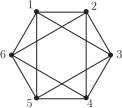
\includegraphics[width=0.33\linewidth]{images/NumberedHexagonalNetwork}
\caption{A graph on six vertices.\label{starhexagon}}
\end{figure}
~{\tiny (h)}~{\tiny (h)}\end{activity}
\typeout{************************************************}
\typeout{Section 6.3 Pólya-Redfield Enumeration Theory}
\typeout{************************************************}
\section[{Pólya-Redfield Enumeration Theory}]{Pólya-Redfield Enumeration Theory}\label{sec_groups-polya}
\hypertarget{p-1729}{}%
George Pólya and Robert Redfield independently developed a theory of generating functions that describe the action of a group \(G\) on functions from a set \(S\) to a set \(T\) when we know the action of \(G\) on \(S\). Pólya's work on the subject is very accessible in its exposition, and so the subject has become popularly known as Pólya theory, though Pólya-Redfield theory would be a better name. In this section we develop the elements of this theory.%
\par
\hypertarget{p-1730}{}%
The idea of coloring a set \(S\) has many applications. For example, the set \(S\) might be the positions in a hydrocarbon molecule which are occupied by hydrogen, and the group could be the group of spatial symmetries of the molecule (that is, the group of permutations of the atoms of the molecule that move the molecule around so that in its final position the molecule cannot be distinguished from the original molecule). The colors could then be radicals (including hydrogen itself) that we could substitute for each hydrogen position in the molecule. Then the number of orbits of colorings is the number of chemically different compounds we could create by using these substitutions.\footnote{There is a fascinating subtle issue of what makes two molecules different.  For example, suppose we have a molecule in the form of a cube, with one atom at each vertex.  If we interchange the top and bottom faces of the cube, each atom is still connected to exactly the same atoms as before.   However we cannot achieve this permutation of the vertices by a member of the rotation group of the cube.  It could well be that the two versions of the molecule interact with other molecules in different ways, in which case we would consider them chemically different.  On the other hand if the two versions interact with other molecules in the same way, we would have no reason to consider them chemically different.  This kind of symmetry is an example of what is called \terminology{chirality} in chemistry.\label{fn-24}}%
\par
\hypertarget{p-1731}{}%
In \hyperref[butyl-alcohol-isomers]{Figure~\ref{butyl-alcohol-isomers}} we show two different ways to substitute the OH radical for a hydrogen atom in the chemical diagram we gave for butane in \hyperref[InductionRecursion]{Chapter~\ref{InductionRecursion}}. We have colored one vertex of degree 1 with the radical OH and the rest with the atom H. There are only two distinct ways to do this, as the OH must either connect to an ``end'' C or a ``middle'' C. This shows that there are two different forms, called isomers of the compound shown. This compound is known as butyl alcohol.%
\begin{figure}
\centering
% group protects changes to lengths, releases boxes (?)
{% begin: group for a single side-by-side
% set panel max height to practical minimum, created in preamble
\setlength{\panelmax}{0pt}
\ifdefined\panelboxAimage\else\newsavebox{\panelboxAimage}\fi%
\begin{lrbox}{\panelboxAimage}
\resizebox{0.47\linewidth}{!}{{
\chemfig{H-[:0]C(-[:90]H)(-[:270]H)-[:0]C(-[:90]H)(-[:270]H)-[:0]C(-[:90]H)(-[:270]OH)-[:0]C(-[:90]H)(-[:270]H)-[:0]H}
}
}\end{lrbox}
\ifdefined\phAimage\else\newlength{\phAimage}\fi%
\setlength{\phAimage}{\ht\panelboxAimage+\dp\panelboxAimage}
\settototalheight{\phAimage}{\usebox{\panelboxAimage}}
\setlength{\panelmax}{\maxof{\panelmax}{\phAimage}}
\ifdefined\panelboxBimage\else\newsavebox{\panelboxBimage}\fi%
\begin{lrbox}{\panelboxBimage}
\resizebox{0.47\linewidth}{!}{{
\chemfig{H-[:0]C(-[:90]H)(-[:270]H)-[:0]C(-[:90]H)(-[:270]H)-[:0]C(-[:90]H)(-[:270]H)-[:0]C(-[:90]H)(-[:270]H)-[:0]OH}
}
}\end{lrbox}
\ifdefined\phBimage\else\newlength{\phBimage}\fi%
\setlength{\phBimage}{\ht\panelboxBimage+\dp\panelboxBimage}
\settototalheight{\phBimage}{\usebox{\panelboxBimage}}
\setlength{\panelmax}{\maxof{\panelmax}{\phBimage}}
\leavevmode%
% begin: side-by-side as tabular
% \tabcolsep change local to group
\setlength{\tabcolsep}{0.015\linewidth}
% @{} suppress \tabcolsep at extremes, so margins behave as intended
\par\medskip\noindent
\hspace*{0.015\linewidth}%
\begin{tabular}{@{}*{2}{c}@{}}
\begin{minipage}[c][\panelmax][t]{0.47\linewidth}\usebox{\panelboxAimage}\end{minipage}&
\begin{minipage}[c][\panelmax][t]{0.47\linewidth}\usebox{\panelboxBimage}\end{minipage}\end{tabular}\\
% end: side-by-side as tabular
}% end: group for a single side-by-side
\caption{The two different isomers of butyl alcohol.\label{butyl-alcohol-isomers}}
\end{figure}
\hypertarget{p-1732}{}%
So think intuitively about some ``figure'' that has places to be colored. (Think of the faces of a cube, the beads on a necklace, circles at the vertices of an \(n\)-gon, etc.) How can we picture the coloring? If we number the places to be colored, say 1 to \(n\), then a function from \([n]\) to the colors is exactly our coloring; if our colors are blue, green and red, then \(BBGRRGBG\) describes a typical coloring of 8 such places. Unless the places are somehow ``naturally'' numbered, this idea of a coloring imposes structure that is not really there. Even if the structure is there, visualizing our colorings in this way doesn't ``pull together'' any common features of different colorings; we are simply visualizing all possible functions. We have a group (think of it as symmetries of the figure you are imagining) that acts on the places. That group then acts in a natural way on the colorings of the places and we are interested in orbits of the colorings. Thus we want a picture that pulls together the common features of the colorings in an orbit. One way to pull together similarities of colorings would be to let the letters we are using as pictures of colors commute as we did with our pictures in \hyperref[ch_genfns]{Chapter~\ref{ch_genfns}}; then our picture \(BBGRRGBG\) becomes \(B^3G^3R^2\), so our picture now records simply how many times we use each color. If you think about how we defined the action of a group on a set of functions, you will see that a group element won't change how many times each color is used; it simply moves colors to different places. Thus the picture we now have of a given coloring is an equally appropriate picture for each coloring in an orbit. One natural question for us to ask is ``How many orbits have a given picture?''%
\begin{activity}[]\marginsymbol[-1em]{} \label{coloredhex}
\hypertarget{p-1733}{}%
Suppose we draw identical circles at the vertices of a regular hexagon. Suppose we color these circles with two colors, red and blue.%
\begin{enumerate}[font=\bfseries,label=(\alph*),ref=\alph*]
\item\label{task-230} \marginsymbol[-2.5em]{} \hypertarget{p-1734}{}%
In how many ways may we color the set \(\{1, 2, 3, 4, 5, 6\}\) using the colors red and blue?%
\item\label{task-231} \marginsymbol[-2.5em]{} \hypertarget{p-1736}{}%
These colorings are partitioned into orbits by the action of the rotation group on the hexagon. Using our standard notation, write down all these orbits and observe how many orbits have each picture, assuming the picture of a coloring is the product of commuting variables representing the colors.%
\item\label{picture-enumerator-hexagon} \marginsymbol[-2.5em]{} \hypertarget{p-1739}{}%
Using the picture function of the previous part, write down the picture enumerator for the orbits of colorings of the vertices of a hexagon under the action of the rotation group.%
\end{enumerate}
\end{activity}
\hypertarget{p-1741}{}%
In \hyperref[picture-enumerator-hexagon]{Problem~c} we saw a picture enumerator for pictures of orbits of the action of a group on colorings. As above, we can ask how many orbits of the colorings have any given picture. We can think of a multivariable generating function in which the letters we use to picture individual colors are the variables, and the coefficient of a picture is the number of orbits with that picture. Such a generating function is an answer to our natural question, and so it is this sort of generating function we will seek. Since the CFB theorem was our primary tool for saying how many orbits we have, it makes sense to think about whether the CFB theorem has an analog in terms of pictures of orbits.%
\typeout{************************************************}
\typeout{Subsection 6.3.1 The Orbit-Fixed Point Theorem}
\typeout{************************************************}
\subsection[{The Orbit-Fixed Point Theorem}]{The Orbit-Fixed Point Theorem}\label{subsection-68}
\begin{activity}[]\marginsymbol[-1em]{\pdftooltip{$\bullet$}{essential}} \label{orbit-fixed-point-thm}
\hypertarget{p-1742}{}%
Suppose now we have a group \(G\) acting on a set and we have a picture function on that set with the additional feature that for each orbit of the group, all its elements have the same picture. In this circumstance we define the picture of an orbit or multiorbit to be the picture of any one of its members. The \terminology{orbit enumerator}\index{orbit enumerator}\index{enumerator!orbit} \(\Orb(G,S)\) is the sum of the pictures of the orbits. (Note that this is the same as the sum of the pictures of the \terminology{multiorbits}\index{multiorbits}.) The \terminology{fixed point enumerator}\index{fixed point enumerator}\index{enumerator!fixed point} \(\Fix(G, S)\) is the sum of the pictures of each of the fixed points of each of the elements of \(G\). We are going to construct a generating function analog of the CFB theorem. The main idea of the proof of the CFB theorem was to try to compute in two different ways the number of elements (i.e. the sum of all the multiplicities of the elements) in the union of all the multiorbits of a group acting on a set. Suppose instead we try to compute the sum of all the pictures of all the elements in the union of the multiorbits of a group acting on a set. By thinking about how this sum relates to \(\Orb(G,S)\) and \(\Fix(G,S)\), find an analog of the CFB theorem that relates these two enumerators. State and prove this theorem. \index{Orbit-Fixed Point Theorem}%
\end{activity}
\hypertarget{p-1744}{}%
We call the theorem of \hyperref[orbit-fixed-point-thm]{Problem~\ref{orbit-fixed-point-thm}} the \terminology{Orbit-Fixed Point Theorem}. In order to apply the Orbit-Fixed Point Theorem, we need some facts about picture enumerators.\index{Orbit-Fixed Point Theorem}%
\begin{activity}[]\marginsymbol[-1em]{\pdftooltip{$\bullet$}{essential}} \label{ProdPrincPictureEnumerators}
\hypertarget{p-1745}{}%
Suppose that \(P_1\) and \(P_2\) are picture functions on sets \(S_1\) and \(S_2\) in the sense of \hyperref[picturefunction]{Section~\ref{picturefunction}}. Define \(P\) on \(S_1 \times
S_2\) by \(P(x_1,x_2) = P_1(x_1)P_2(x_2)\). How are \(E_{P_1}\), \(E_{P_1}\), and \(E_{P}\) related? (You may have already done this problem in another context!)%
\end{activity}
\begin{activity}[]\marginsymbol[-1em]{\pdftooltip{$\bullet$}{essential}} \label{PictureEnumeratorforFunctions}
\hypertarget{p-1747}{}%
Suppose \(P_i\) is a picture function on a set \(S_i\) for \(i=1,\dots,k\). We define the picture of a \(k\)-tuple \((x_1,x_2,\dots,x_k)\) to be the product of the pictures of its elements, i.e.\@%
\begin{equation*}
\widehat P((x_1,x_2,\dots,x_k)) = \prod_{i=1}^k P_i(x_i).
\end{equation*}
%
\par
\hypertarget{p-1748}{}%
How does the picture enumerator \(E_{\widehat P}\) of the set \(S_1\times S_2\times\cdots\times S_k\) of all \(k\)-tuples with \(x_i\in S\) relate to the picture enumerators of the sets \(S_i\)? In the special case that \(S_i = S\) for all \(i\) and \(P_i = P\) for all \(i\), what is \(E_{\widehat{P}}(S^k)\)?%
\end{activity}
\begin{activity}[]\marginsymbol[-1em]{\pdftooltip{$\bullet$}{essential}} \label{polya1}
\hypertarget{p-1750}{}%
Use the Orbit-Fixed Point Theorem to determine the Orbit Enumerator for the colorings, with two colors (red and blue), of six circles placed at the vertices of a hexagon which is free to move in the plane. Compare the coefficients of the resulting polynomial with the various orbits you found in \hyperref[coloredhex]{Problem~\ref{coloredhex}}.%
\end{activity}
\begin{activity}[]\marginsymbol[-1em]{} \label{polya2}
\hypertarget{p-1755}{}%
Find the generating function (in variables \(R\), \(B\)) for colorings of the faces of a cube with two colors (red and blue). What does the generating function tell you about the number of ways to color the cube (up to spatial movement) with various combinations of the two colors.%
\end{activity}
\typeout{************************************************}
\typeout{Subsection 6.3.2 The Pólya-Redfield Theorem}
\typeout{************************************************}
\subsection[{The Pólya-Redfield Theorem}]{The Pólya-Redfield Theorem}\label{subsection-69}
\hypertarget{p-1758}{}%
Pólya's (and Redfield's) famed enumeration theorem deals with situations such as those in \hyperref[polya1]{Problems~\ref{polya1}} and \hyperref[polya2]{Problem~\ref{polya2}} in which we want a generating function for the set of all functions from a set \(S\) to a set \(T\) on which a picture function is defined, and the picture of a function is the product of the pictures of its multiset of values. The point of the next series of problems is to analyze the solution to \hyperref[polya1]{Problems~\ref{polya1}} and \hyperref[polya2]{Problem~\ref{polya2}} in order to see what Pólya and Redfield saw (though they didn't see it in this notation or using this terminology).%
\begin{activity}[]\marginsymbol[-1em]{\pdftooltip{$\bullet$}{essential}} \label{polya3}
\hypertarget{p-1759}{}%
In \hyperref[polya1]{Problem~\ref{polya1}} we have four kinds of group elements: the identity (which fixes every coloring), the rotations through 60 or 300 degrees, the rotations through 120 and 240 degrees, and the rotation through 180 degrees. The fixed point enumerator for the rotation group acting on the functions is by definition the sum of the fixed point enumerators of colorings fixed by the identity, of colorings fixed by 60 or 300 degree rotations, of colorings fixed by 120 or 240 degree rotations, and of colorings fixed by the 180 degree rotation. Write down each of these enumerators (one for each kind of permutation) individually and factor each one (over the integers) as completely as you can.%
\end{activity}
\begin{activity}[]\marginsymbol[-1em]{\pdftooltip{$\bullet$}{essential}} \label{polya4}
\hypertarget{p-1761}{}%
In \hyperref[polya2]{Problem~\ref{polya2}} we have five different kinds of group elements, and the fixed point enumerator is the sum of the fixed point enumerators of each of these kinds of group elements. For each kind of element, write down the fixed point enumerator for the elements of that kind. Factor the enumerators as completely as you can.%
\end{activity}
\begin{activity}[]\marginsymbol[-1em]{\pdftooltip{$\bullet$}{essential}} \label{polya3_5}
\hypertarget{p-1763}{}%
In \hyperref[polya3]{Problem~\ref{polya3}}, each ``kind'' of group element has a ``kind'' of cycle structure. For example, a rotation through 180 degrees has three cycles of size two. What kind of cycle structure does a rotation through 60 or 300 degrees have? What kind of cycle structure does a rotation through 120 or 240 degrees have? Discuss the relationship between the cycle structures and the factored enumerators of fixed points of the permutations in \hyperref[polya3]{Problem~\ref{polya3}}.%
\end{activity}
\hypertarget{p-1765}{}%
Recall that we said that a group of permutations acts on a set if, for each member \(\sigma\) of \(G\) there is a bijection \(\overline{\sigma}\) of \(S\) such that%
\begin{equation*}
\overline{\sigma\circ\varphi} = \overline{\sigma}\circ\overline{\varphi}
\end{equation*}
for every member \(\sigma\) and \(\varphi\) of \(G\). Since \(\overline{\sigma}\) is a bijection of \(S\) to itself, it is in fact a permutation of \(S\). Thus \(\overline{\sigma}\) has a cycle structure (that is, it is a product of disjoint cycles) as a permutation of \(S\) (in addition to whatever its cycle structure is in the original permutation group \(G\)).%
\begin{activity}[]\marginsymbol[-1em]{\pdftooltip{$\bullet$}{essential}} \label{activity-319}
\hypertarget{p-1766}{}%
In \hyperref[polya4]{Problem~\ref{polya4}}, each ``kind'' of group element has a ``kind'' of cycle structure in the action of the rotation group of the cube on the faces of the cube. For example, a rotation of the cube through 180 degrees around a vertical axis through the centers of the top and bottom faces has two cycles of size two and two cycles of size one. How many such rotations does the group have? What are the other ``kinds'' of group elements, and what are their cycle structures? Discuss the relationship between the cycle structure and the factored enumerator in \hyperref[polya4]{Problem~\ref{polya4}}.%
\end{activity}
\begin{activity}[]\marginsymbol[-1em]{\pdftooltip{$\bullet$}{essential}} \label{activity-320}
\hypertarget{p-1772}{}%
The usual way of describing the Pólya-Redfield enumeration theorem involves the ``cycle indicator'' or ``cycle index'' of a group acting on a set. Suppose we have a group \(G\) acting on a finite set \(S\). Since each group element \(\sigma\) gives us a permutation \(\overline{\sigma}\) of \(S\), as such it has a decomposition into disjoint cycles as a permutation of \(S\). Suppose \(\sigma\) has \(c_1\) cycles of size 1, \(c_2\) cycles of size 2, ..., \(c_n\) cycles of size \(n\). Then the \terminology{cycle monomial}\index{cycle monomial} of \(\sigma\) is%
\begin{equation*}
z(\sigma) = z_1^{c_1}z_2^{c_2}\cdots z_n^{c_n}.
\end{equation*}
%
\par
\hypertarget{p-1773}{}%
The \terminology{cycle indicator} or \terminology{cycle index}\index{cycle index} of \(G\) acting on \(S\) is%
\begin{equation*}
Z(G,S) = \frac{1}{|G|}\sum_{\sigma: \sigma \in G} z(\sigma).
\end{equation*}
%
\begin{enumerate}[font=\bfseries,label=(\alph*),ref=\alph*]
\item\label{task-233} \marginsymbol[-2.5em]{} \hypertarget{p-1774}{}%
What is the cycle index for the group \(D_6\) acting on the vertices of a hexagon?%
\item\label{task-234} \marginsymbol[-2.5em]{} \hypertarget{p-1776}{}%
What is the cycle index for the group of rotations of the cube acting on the faces of the cube?%
\end{enumerate}
\end{activity}
\begin{activity}[]\marginsymbol[-1em]{} \label{activity-321}
\hypertarget{p-1778}{}%
How can you compute the Orbit Enumerator of \(G\) acting on functions from \(S\) to a finite set \(T\) from the cycle index of \(G\) acting on \(S\)? (Use \(t\), thought of as a variable, as the picture of an element \(t\) of \(T\).) State and prove the relevant theorem! This is Pólya's and Redfield's famous enumeration theorem.\index{Pólya-Redfield Theorem}%
\end{activity}
\begin{activity}[]\marginsymbol[-1em]{\pdftooltip{$\importantarrow$}{especially interesting}} \label{activity-322}
\hypertarget{p-1780}{}%
Suppose we make a necklace by stringing 12 pieces of brightly colored plastic tubing onto a string and fastening the ends of the string together. We have ample supplies blue, green, red, and yellow tubing available. Give a generating function in which the coefficient of \(B^iG^jR^kY^h\) is the number of necklaces we can make with \(i\) blues, \(j\) greens, \(k\) reds, and \(h\) yellows. How many terms would this generating function have if you expanded it in terms of powers of \(B\), \(G\), \(R\), and \(Y\)? Does it make sense to do this expansion? How many of these necklaces have 3 blues, 3 greens, 2 reds, and 4 yellows?%
\end{activity}
\begin{activity}[]\marginsymbol[-1em]{} \label{activity-323}
\hypertarget{p-1785}{}%
What should we substitute for the variables representing colorings in the orbit enumerator of \(G\) acting on the set of colorings of \(S\) by a set \(T\) of colors in order to compute the total number of orbits of \(G\) acting on the set of colorings? What should we substitute into the variables in the cycle index of a group \(G\) acting on a set \(S\) in order to compute the total number of orbits of \(G\) acting on the colorings of \(S\) by a set \(T\)? Find the number of ways to color the faces of a cube with four colors.%
\end{activity}
\begin{activity}[]\marginsymbol[-1em]{\pdftooltip{$\importantarrow$}{especially interesting}} \label{coloredsticks}
\hypertarget{p-1788}{}%
We have red, green, and blue sticks all of the same length, with a dozen sticks of each color. We are going to make the skeleton of a cube by taking eight identical lumps of modeling clay and pushing three sticks into each lump so that the lumps become the vertices of the cube. (Clearly we won't need all the sticks!) In how many different ways could we make our cube? How many cubes have four edges of each color? How many have two red, four green, and six blue edges?%
\end{activity}
\begin{activity}[]\marginsymbol[-1em]{\pdftooltip{$\importantarrow$}{especially interesting}} \label{activity-325}
\hypertarget{p-1794}{}%
How many cubes can we make in \hyperref[coloredsticks]{Problem~\ref{coloredsticks}} if the lumps of modelling clay can be any of four colors?%
\end{activity}
\begin{figure}
\centering
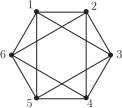
\includegraphics[width=0.33\linewidth]{images/NumberedHexagonalNetwork}
\caption{A possible computer network.\label{HexNet}}
\end{figure}
\begin{activity}[]\marginsymbol[-1em]{\pdftooltip{$\importantarrow$}{especially interesting}} \label{activity-326}
\hypertarget{p-1798}{}%
In \hyperref[HexNet]{Figure~\ref{HexNet}} we see a graph with six vertices. Suppose we have three different kinds of computers that can be placed at the six vertices of the graph to form a network. In how many different ways may the computers be placed? (Two graphs are not different if we can redraw one of the graphs so that it is identical to the other one.) This is equivalent to permuting the vertices in some way so that when we apply the permutation to the endpoints of the edges to get a new edge set, the new edge set is equal to the old one. Such a permutation is called an \terminology{automorphism}\index{automorphism (of a graph)} of the graph. Then two computer placements are the same if there is an automorphism of the graph that carries one to the other.%
~{\tiny (h)}~{\tiny (h)}\end{activity}
\begin{activity}[]\marginsymbol[-1em]{\pdftooltip{$\importantarrow$}{especially interesting}} \label{activity-327}
\hypertarget{p-1805}{}%
Two simple graphs on the set \([n]= \{1,2,\ldots, n\}\) with edge sets \(E\) and \(E'\) (which we think of a sets of two-element sets for this problem) are said to be \terminology{isomorphic}\index{graphs!isomorphic}\index{isomorphic!graphs} if there is a permutation \(\sigma\) of \([n]\) which, in its action of two-element sets, carries \(E\) to \(E'\). We say two graphs are different if they are not isomorphic. Thus the number of different graphs is the number of orbits of the set of all two-element subsets of \([n]\) under the action of the group \(S_n\). We can represent an edge set by its characteristic function (as in \hyperref[charfunction]{problem~\ref{charfunction}}). That is we define%
\begin{equation*}
\chi_E(\{u,v\}) = \left\{
\begin{array}{ll}
1 \amp  \mbox{if \(\{u,v\}\in E\)} \\
0 \amp  \mbox{otherwise.}
\end{array} \right.
\end{equation*}
%
\par
\hypertarget{p-1806}{}%
Thus we can think of the set of graphs as a set of colorings with colors 0 and 1 of the set of all two-element subsets of \([n]\). The number of different graphs with vertex set \([n]\) is thus the number of orbits of this set of colorings under the action of the symmetric group \(S_n\) on the set of two-element subsets of \([n]\). Use this to find the number of different graphs on five vertices.%
~{\tiny (h)}\end{activity}
\typeout{************************************************}
\typeout{Supplementary Problems 6.4 Supplementary Problems}
\typeout{************************************************}
\section[{Supplementary Problems}]{Supplementary Problems}\label{sec_groups-suppprobs}
\begin{exerciselist}
\item[1.]\marginsymbol[-1em]{} \hypertarget{exercise-54}{}\hypertarget{p-1817}{}%
Show that a function from \(S\) to \(T\) has an inverse (defined on \(T\)) if and only if it is a bijection.%
\par\smallskip
\item[2.]\marginsymbol[-1em]{} \hypertarget{exercise-55}{}\hypertarget{p-1818}{}%
How many elements are in the dihedral group \(D_3\)?  The symmetric group \(S_3\)?  What can you conclude about \(D_3\) and \(S_3\)?%
\par\smallskip
\item[3.]\marginsymbol[-1em]{} \hypertarget{exercise-56}{}\hypertarget{p-1820}{}%
A tetrahedron is a thee dimensional geometric figure with four vertices, six edges, and four triangular faces.  Suppose we start with a tetrahedron in space and consider the set of all permutations of the vertices of the tetrahedron that correspond to moving the tetrahedron in space and returning it to its original location, perhaps with the vertices in different places. \leavevmode%
\begin{enumerate}[label=(\alph*)]
\item\hypertarget{li-117}{}Explain why these permutations form a group.%
\item\hypertarget{li-118}{}What is the size of this group?%
\item\hypertarget{li-119}{}Write down in two-row notation a permutation that is \emph{not} in this group.%
\end{enumerate}
%
\par\smallskip
\item[4.]\marginsymbol[-1em]{} \hypertarget{exercise-57}{}\hypertarget{p-1821}{}%
Find a three-element subgroup of the group \(S_3\).  Can you find a different three-element subgroup of \(S_3\)?%
\par\smallskip
\item[5.]\marginsymbol[-1em]{} \hypertarget{exercise-58}{}\hypertarget{p-1823}{}%
Prove true or demonstrate false with a counterexample: ``In a permutation group, \((\sigma\varphi)^n = \sigma^n\varphi^n\).''%
\par\smallskip
\item[6.]\marginsymbol[-1em]{} \hypertarget{exercise-59}{}\hypertarget{p-1824}{}%
If a group \(G\) acts on a set \(S\), and if \(\sigma(x) =y\), is there anything interesting we can say about the subgroups \(\Fix(x)\) and \(\Fix(y)\)?%
\par\smallskip
\item[7.]\marginsymbol[-1em]{} \hypertarget{exercise-60}{}\hypertarget{p-1826}{}%
\leavevmode%
\begin{enumerate}[label=(\alph*)]
\item\hypertarget{li-120}{}\hypertarget{p-1827}{}%
If a group \(G\) acts on a set \(S\), does \(\overline{\sigma}(f) = f\circ\sigma\) define a group action on the functions from \(S\) to a set \(T\)? Why or why not?%
\item\hypertarget{li-121}{}\hypertarget{p-1828}{}%
If a group \(G\) acts on a set \(S\), does \(\sigma(f)=f\circ\sigma^{-1}\) define a group action on the functions from \(S\) to a set \(T\) ? Why or why not?%
\item\hypertarget{li-122}{}\hypertarget{p-1829}{}%
Is either of the possible group actions essentially the same as the action we described on colorings of a set, or is that an entirely different action?%
\end{enumerate}
%
\par\smallskip
\item[8.]\marginsymbol[-1em]{} \hypertarget{exercise-61}{}\hypertarget{p-1834}{}%
Find the number of ways to color the faces of a tetrahedron with two colors.%
\par\smallskip
\item[9.]\marginsymbol[-1em]{} \hypertarget{exercise-62}{}\hypertarget{p-1835}{}%
Find the number of ways to color the faces of a tetrahedron with four colors so that each color is used.%
\par\smallskip
\item[10.]\marginsymbol[-1em]{} \hypertarget{exercise-63}{}\hypertarget{p-1836}{}%
Find the cycle index of the group of spatial symmetries of the tetrahedron acting on the vertices.  Find the cycle index for the same group acting on the faces.%
\par\smallskip
\item[11.]\marginsymbol[-1em]{} \hypertarget{exercise-64}{}\hypertarget{p-1837}{}%
Find the generating function for the number of ways to color the faces of the tetrahedron with red, blue, green and yellow.%
\par\smallskip
\item[12.]\marginsymbol[-1em]{\pdftooltip{$\importantarrow$}{especially interesting}} \hypertarget{exercise-65}{}\hypertarget{p-1838}{}%
Find the generating function for the number of ways to color the faces of a cube with four colors so that all four colors are used.%
\par\smallskip
\item[13.]\marginsymbol[-1em]{\pdftooltip{$\importantarrow$}{especially interesting}} \hypertarget{exercise-66}{}\hypertarget{p-1839}{}%
How many different graphs are there on six vertices with seven edges?%
\par\smallskip
\item[14.]\marginsymbol[-1em]{\pdftooltip{$\importantarrow$}{especially interesting}} \hypertarget{exercise-67}{}\hypertarget{p-1840}{}%
Show that if \(H\) is a subgroup of the group \(G\), then \(H\) acts on \(G\) by \(\sigma(\tau) = \sigma\circ\tau\) for all \(\sigma\) in \(H\) and \(\tau\) in \(G\). What is the size of an orbit of this action? How does the size of a subgroup of a group relate to the size of the group?%
\par\smallskip
\end{exerciselist}
%
%% A lineskip in table of contents as transition to appendices, backmatter
\addtocontents{toc}{\vspace{\normalbaselineskip}}
%
%
\appendix
%
\typeout{************************************************}
\typeout{Appendix A Relations}
\typeout{************************************************}
\chapter[{Relations}]{Relations}\label{Relations}
\typeout{************************************************}
\typeout{Section A.1 Relations as sets of Ordered Pairs}
\typeout{************************************************}
\section[{Relations as sets of Ordered Pairs}]{Relations as sets of Ordered Pairs}\label{relationsandfunctions}
\typeout{************************************************}
\typeout{Subsection A.1.1 The relation of a function}
\typeout{************************************************}
\subsection[{The relation of a function}]{The relation of a function}\label{functionrelation}
\begin{activity}[]\marginsymbol[-1em]{} \label{functionsasorderedpairs}
\hypertarget{p-1842}{}%
Consider the functions from \(S=\{-2,-1,0,1,2\}\) to \(T=\{1,2,3,4,5\}\) defined by \(f(x) = x+3\), and \(g(x) = x^5-5x^3+5x +3\). Write down the set of ordered pairs \((x,f(x))\) for \(x \in S\) and the set of ordered pairs \((x,g(x))\) for \(x \in S\). Are the two functions the same or different?%
\end{activity}
\hypertarget{p-1844}{}%
\hyperref[functionsasorderedpairs]{Problem~\ref{functionsasorderedpairs}} points out how two functions which appear to be different are actually the same on some domain of interest to us. Most of the time when we are thinking about functions it is fine to think of a function casually as a relationship between two sets. In \hyperref[functionsasorderedpairs]{Problem~\ref{functionsasorderedpairs}} the set of ordered pairs you wrote down for each function is called the \index{relation!of a function}\index{function!relation of}\terminology{relation} of the function. When we want to distinguish between the casual and the careful in talking about relationships, our casual term will be ``relationship'' and our careful term will be ``relation.'' So \emph{relation} is a technical word in mathematics, and as such it has a technical definition. A \index{relation}\terminology{relation} from a set \(S\) to a set \(T\) is a set of ordered pairs whose first elements are in \(S\) and whose second elements are in \(T\). Another way to say this is that a \terminology{relation} from \(S\) to \(T\) is a subset of \(S\times T\).%
\par
\hypertarget{p-1845}{}%
A typical way to define a \terminology{function}\index{function} \(f\) from a set \(S\), called the \terminology{domain} of the function, \index{domain (of a function)} to a set \(T\), called the \terminology{range}, \index{range (of a function)} is that \(f\) is a relationship between \(S\) to \(T\) that relates one and only one member of \(T\) to each element of \(X\). We use \(f(x)\) to stand for the element of \(T\) that is related to the element \(x\) of \(S\). If we wanted to make our definition more precise, we could substitute the word ``relation'' for the word ``relationship'' and we would have a more precise definition. For our purposes, you can choose whichever definition you prefer. However, in any case, there is a relation associated with each function. As we said above, the relation of a function \(f:
S\rightarrow T\) (which is the standard shorthand for ``\(f\) is a function from \(S\) to \(T\)'' and is usually read as \(f\) \terminology{maps} \(S\) to \(T\)) is the set of all ordered pairs \((x,f(x))\) such that \(x\) is in \(S\).%
\begin{activity}[]\marginsymbol[-1em]{} \label{formalrelations}
\hypertarget{p-1846}{}%
Here are some questions that will help you get used to the formal idea of a relation and the related formal idea of a function. \(S\) will stand for a set of size \(s\) and \(T\) will stand for a set of size \(t\).%
\begin{enumerate}[font=\bfseries,label=(\alph*),ref=\alph*]
\item\label{task-235} \marginsymbol[-2.5em]{} \hypertarget{p-1847}{}%
What is the size of the largest relation from \(S\) to \(T\)?%
\item\label{task-236} \marginsymbol[-2.5em]{} \hypertarget{p-1849}{}%
What is the size of the smallest relation from \(S\) to \(T\)?%
\item\label{task-237} \marginsymbol[-2.5em]{} \hypertarget{p-1851}{}%
The relation of a function \(f:S\rightarrow T\) is the set of all ordered pairs \((x,f(x))\) with \(x\in S\).  What is the size of the relation of a function from \(S\) to \(T\)?  That is, how many ordered pairs are in the relation of a function from \(S\) to \(T\)?%
~{\tiny (h)}\item\label{task-238} \marginsymbol[-2.5em]{} \hypertarget{p-1854}{}%
We say \(f\) is a \terminology{one-to-one}\index{function!one-to-one}\index{one-to-one function}\index{injection} function or \terminology{injection} from \(S\) to \(T\) if each member of \(S\) is related to a \emph{different} element of \(T\). How many different elements must appear as second elements of the ordered pairs in the relation of a one-to-one function (injection) from \(S\) to \(T\)?%
\item\label{onto} \marginsymbol[-2.5em]{} \hypertarget{p-1856}{}%
A function \(f:S\rightarrow T\) is called an \index{onto function}\index{function!onto}\terminology{onto function} or \index{surjection}\index{function!surjection}\terminology{surjection} if each element of \(T\) is \(f(x)\) for some \(x\in S\) What is the minimum size that \(S\) can have if there is a  surjection from \(S\) to \(T\)?%
\end{enumerate}
\end{activity}
\begin{activity}[]\marginsymbol[-1em]{} \label{activity-330}
\hypertarget{p-1858}{}%
When \(f\) is a function from \(S\) to \(T\), the sets \(S\) and \(T\) play a big role in determining whether a function is one-to-one or onto (as defined in \hyperref[formalrelations]{Problem~\ref{formalrelations}}). For the remainder of this problem, let \(S\) and \(T\) stand for  the set of nonnegative real numbers.%
\begin{enumerate}[font=\bfseries,label=(\alph*),ref=\alph*]
\item\label{task-240} \marginsymbol[-2.5em]{} \hypertarget{p-1859}{}%
If \(f:S\rightarrow T\) is given by \(f(x) =x^2\), is \(f\) one-to-one? Is \(f\) onto?%
\item\label{task-241} \marginsymbol[-2.5em]{} \hypertarget{p-1861}{}%
Now assume \(S'\) is the set of all real numbers and \(g:S'\rightarrow T\) is given by \(g(x) = x^2\). Is \(g\) one-to-one? Is \(g\) onto?%
\item\label{task-242} \marginsymbol[-2.5em]{} \hypertarget{p-1863}{}%
Assume that \(T'\) is the set of all real numbers and \(h:S\rightarrow T'\) is given by \(h(x) = x^2\). Is \(h\) one-to-one? Is \(h\) onto?%
\item\label{task-243} \marginsymbol[-2.5em]{} \hypertarget{p-1865}{}%
And if the function \(j:S'\rightarrow T'\) is given by \(j(x)=x^2\), is \(j\) one-to-one? Is \(j\) onto?%
\end{enumerate}
\end{activity}
\begin{activity}[]\marginsymbol[-1em]{} \label{activity-331}
\hypertarget{p-1867}{}%
If \(f:S\rightarrow T\) is a function, we say that \(f\) \terminology{maps} \(x\) to \(y\) as another way to say that \(f(x)=y\). Suppose \(S=T=\{1,2,3\}\). Give a function from \(S\) to \(T\) that is not onto. Notice that two different members of \(S\) have mapped to the same element of \(T\). Thus when we say that \(f\) associates one and only one element of \(T\) to each element of \(S\), it is quite possible that the one and only one element \(f(1)\) that \(f\) maps 1 to is exactly the same as the one and only one element \(f(2)\) that \(f\) maps 2 to.%
\end{activity}
\typeout{************************************************}
\typeout{Subsection A.1.2 Directed graphs}
\typeout{************************************************}
\subsection[{Directed graphs}]{Directed graphs}\label{relationdigraph}
\hypertarget{p-1869}{}%
We visualize numerical functions like \(f(x)=x^2\) with their graphs in Cartesian coordinate systems. We will call these kinds of graphs \index{graph!coordinate}\emph{coordinate graphs} to distinguish them from other kinds of graphs used to visualize relations that are non-numerical.%
\begin{figure}
\centering
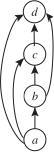
\includegraphics[width=0.1\linewidth]{images/alphabetdigraph}
\caption{The alphabet digraph.\label{alphabetdigraph}}
\end{figure}
\hypertarget{p-1870}{}%
In \hyperref[alphabetdigraph]{Figure~\ref{alphabetdigraph}} we illustrate another kind of graph, a ``directed graph'' or ``digraph'' of the ``comes before in alphabetical order" relation on the letters \(a\), \(b\), \(c\), and \(d\). To draw a \index{graph!directed}\index{directed graph}\index{digraph}\terminology{directed graph} of a relation on a set \(S\), we draw a circle (or dot, if we prefer), which we call a \index{vertex}\terminology{vertex}\index{vertex!of a complete graph}, for each element of the set, we usually label the vertex with the set element it corresponds to, and we draw an arrow from the vertex for \(a\) to that for \(b\) if \(a\) is related to \(b\), that is, if the ordered pair \((a,b)\) is in our relation. We call such an arrow an \index{edge}\terminology{edge}\index{edge!in a digraph} or a \terminology{directed edge}. We draw the arrow from \(a\) to \(b\), for example, because \(a\) comes before \(b\) in alphabetical order. We try to choose the locations where we draw our vertices so that the arrows capture what we are trying to illustrate as well as possible. Sometimes this entails redrawing our directed graph several times until we think the arrows capture the relationship well.%
\par
\hypertarget{p-1871}{}%
We also draw digraphs for relations from a set \(S\) to a set \(T\); we simply draw vertices for the elements of \(S\) (usually in a row) and vertices for the elements of \(T\) (usually in a parallel row) draw an arrow from \(x\) in \(S\) to \(y\) in \(T\) if \(x\) is related to \(y\). Notice that instead of referring to the vertex representing \(x\), we simply referred to \(x\). This is a common shorthand. Here are some exercises just to practice drawing digraphs.%
\begin{activity}[]\marginsymbol[-1em]{} \label{activity-332}
\hypertarget{p-1872}{}%
Draw the digraph of the ``is a proper subset of'' relation on the set of subsets of a two element set. How many arrows would you have had to draw if this problem asked you to draw the digraph for the subsets of a three-element set?%
~{\tiny (h)}\end{activity}
\hypertarget{p-1875}{}%
We also draw digraphs for relations from finite set \(S\) to a finite set \(T\); we simply draw vertices for the elements of \(S\) (usually in a row) and vertices for the elements of \(T\) (usually in a parallel row) and draw an arrow from \(x\) in \(S\) to \(y\) in \(T\) if \(x\) is related to \(y\). Notice that instead of referring to the vertex representing \(x\), we simply referred to \(x\). This is a common shorthand.%
\begin{activity}[]\marginsymbol[-1em]{} \label{initialdigraph}
\hypertarget{p-1876}{}%
Draw the digraph of the relation from the set \{A, M, P, S\} to the set \{Sam, Mary, Pat, Ann, Polly, Sarah\} given by ``is the first letter of.''%
\end{activity}
\begin{activity}[]\marginsymbol[-1em]{} \label{initialdigraph2}
\hypertarget{p-1877}{}%
Draw the digraph of the relation from the set \{Sam, Mary, Pat, Ann, Polly, Sarah\} to the set \{A, M, P, S\} given by ``has as its first letter.''%
\end{activity}
\begin{activity}[]\marginsymbol[-1em]{} \label{activity-335}
\hypertarget{p-1878}{}%
Draw the digraph of the relation on the set \{Sam, Mary, Pat, Ann, Polly, Sarah\} given by ``has the same first letter as.''%
\end{activity}
\typeout{************************************************}
\typeout{Subsection A.1.3 Digraphs of Functions}
\typeout{************************************************}
\subsection[{Digraphs of Functions}]{Digraphs of Functions}\label{digraphsoffunctions}
\begin{activity}[]\marginsymbol[-1em]{} \label{activity-336}
\hypertarget{p-1879}{}%
When we draw the digraph of a function \(f\), we draw an arrow \emph{from} the vertex representing \(x\) \emph{to} the vertex representing \(f(x)\).  One of the relations you considered in \hyperref[initialdigraph]{Problems~\ref{initialdigraph}} and \hyperref[initialdigraph2]{Problem~\ref{initialdigraph2}} is the relation of a function.%
\begin{enumerate}[font=\bfseries,label=(\alph*),ref=\alph*]
\item\label{task-244} \marginsymbol[-2.5em]{} \hypertarget{p-1880}{}%
Which relation is the relation of a function?%
\item\label{task-245} \marginsymbol[-2.5em]{} \hypertarget{p-1882}{}%
How does the digraph help you visualize that one relation is a function and the other is not?%
\end{enumerate}
\end{activity}
\begin{activity}[]\marginsymbol[-1em]{} \label{functiondigraphs-prob}
\hypertarget{p-1884}{}%
Digraphs of functions help us to visualize whether or not they are onto or one-to-one. For example, let both \(S\) and \(T\) be the set \(\{-2, -1, 0 ,1, 2\}\) and let \(S'\) and \(T'\) be the set \(\{0,1,2\}\).  Let \(f(x) = 2-|x|\).%
\begin{enumerate}[font=\bfseries,label=(\alph*),ref=\alph*]
\item\label{task-246} \marginsymbol[-2.5em]{} \hypertarget{p-1885}{}%
Draw the digraph of the function \(f\) assuming its domain is \(S\) and its range is \(T\).  Use the digraph to explain why or why not this function maps \(S\) onto \(T\).%
\item\label{task-247} \marginsymbol[-2.5em]{} \hypertarget{p-1887}{}%
Use the digraph of the previous part to explain whether or not the function is one-to one.%
\item\label{task-248} \marginsymbol[-2.5em]{} \hypertarget{p-1889}{}%
Draw the digraph of the function \(f\) assuming its domain is \(S\) and its range is \(T'\). Use the digraph to explain whether or not the function is onto.%
\item\label{task-249} \marginsymbol[-2.5em]{} \hypertarget{p-1891}{}%
Use the digraph of the previous part to explain whether or not the function is one-to-one.%
\item\label{task-250} \marginsymbol[-2.5em]{} \hypertarget{p-1893}{}%
Draw the digraph of the function \(f\) assuming its domain is \(S'\) and its range is \(T'\). Use the digraph to explain whether the function is onto.%
\item\label{task-251} \marginsymbol[-2.5em]{} \hypertarget{p-1895}{}%
Use the digraph of the previous part to explain whether the function is one-to-one.%
\item\label{task-252} \marginsymbol[-2.5em]{} \hypertarget{p-1897}{}%
Suppose the function \(f\) has domain \(S'\) and range \(T\).  Draw the digraph of \(f\) and use it to explain whether \(f\) is onto.%
\item\label{task-253} \marginsymbol[-2.5em]{} \hypertarget{p-1899}{}%
Use the digraph of the previous part to explain whether \(f\) is one-to-one.%
\end{enumerate}
\end{activity}
\hypertarget{p-1901}{}%
A one-to-one function from a set \(X\) onto a set \(Y\) is frequently called a \terminology{bijection}\index{bijection}, especially in combinatorics.  Your work in \hyperref[functiondigraphs-prob]{Problem~\ref{functiondigraphs-prob}} should show you that a digraph is the digraph of a bijection from \(X\) to \(Y\) \leavevmode%
\begin{itemize}[label=\textbullet]
\item{}\hypertarget{p-1902}{}%
if the vertices of the digraph represent the elements of \(X\) and \(Y\),%
\item{}\hypertarget{p-1903}{}%
if each vertex representing an element of \(X\) has one and only one arrow leaving it, and%
\item{}\hypertarget{p-1904}{}%
each vertex representing an element of \(Y\) has one and only one arrow entering it.%
\end{itemize}
%
\begin{activity}[]\marginsymbol[-1em]{} \label{activity-338}
\hypertarget{p-1905}{}%
If we reverse all the arrows in the digraph of a bijection \(f\), we get the digraph of another function \(g\). Is \(g\) a bijection? What is \(f(g(x))\)? What is \(g(f(x))\)?%
\end{activity}
\hypertarget{p-1907}{}%
If \(f\) is a function from \(S\) to \(T\), if \(g\) is a function from \(T\) to \(S\), and if \(f(g(x))= x\) for each \(x\) in \(T\) and \(g(f(x)) = x\) for each \(x\) in \(S\), then we say that \(g\) is an inverse of \(f\) (and \(f\) is an inverse of \(g\)).%
\par
\hypertarget{p-1908}{}%
More generally, if \(f\) is a function from a set \(R\) to a set \(S\), and \(g\) is a function from \(S\) to \(T\), then we define a new function \(f \circ g\), called the \terminology{composition} of \(f\) and \(g\) \index{composition}\index{function!composition}, by \(f\circ g(x) = f(g(x))\).  Composition of functions is a particularly important operatio in subjects such as calculus, where we represent a function like \(h(x) = \sqrt{x^2 + 1}\) as the composition of the square root function and the square and add one function in order to use the chain rule to take the derivative of \(h\).%
\par
\hypertarget{p-1909}{}%
The function \(\iota\) (the Greek letter iota is pronounced eye-oh-ta) from a set \(S\) to itself, given by the rule \(\iota(x) = x\) for every \(x\) in \(S\), is called the \terminology{identity function} on S. \index{identity function} If \(f\) is a function from \(S\) to \(T\) and \(g\) is a function from \(T\) to \(S\) such that \(g(f(x)) = x\) for every \(x\) in \(S\), we can express this by saying that \(g\circ f = \iota\), where \(\iota\) is the identity function of \(S\). Saying that \(f(g(x)) = x\) is the same as saying that \(f\circ g = \iota\), where \(\iota\) stands for the identity function on \(T\).  We use the same letter for the identity function on two different sets when we can use context to tell us on which set the identity function is being defined.%
\begin{activity}[]\marginsymbol[-1em]{} \label{activity-339}
\hypertarget{p-1910}{}%
If \(f\) is a function from \(S\) to \(T\) and \(g\) is a function from \(T\) to \(S\) such that \(g(f(x)) = x\), how can we tell from context that \(g\circ f\) is the identity function on \(S\) and not the identity function on \(T\)?%
~{\tiny (h)}\end{activity}
\begin{activity}[]\marginsymbol[-1em]{} \label{inversetobijection}
\hypertarget{p-1913}{}%
Explain why a function that has an inverse must be a bijection.%
\end{activity}
\begin{activity}[]\marginsymbol[-1em]{} \label{activity-341}
\hypertarget{p-1915}{}%
Is it true that the inverse of a bijection is a bijection?%
\end{activity}
\begin{activity}[]\marginsymbol[-1em]{} \label{activity-342}
\hypertarget{p-1917}{}%
If \(g\) and \(h\) are inverse of \(f\), then what can we say about \(g\) and \(h\)?%
\end{activity}
\begin{activity}[]\marginsymbol[-1em]{} \label{activity-343}
\hypertarget{p-1919}{}%
Explain why a bijection must have an inverse.%
\end{activity}
\hypertarget{p-1921}{}%
Since a function with an inverse has exactly one inverse \(g\), we call \(g\) \emph{the} inverse of \(f\).  From now on, when \(f\) has an inverse, we shall denote its inverse by \(f^{-1}\).  Thus \(f(f^{-1}(x)) = x\) and \(f^{-1}(f(x)) = x\).  Equivalenetly \(f\circ f^{-1} = \iota\) and \(f^{-1} \circ f = \iota\).%
\typeout{************************************************}
\typeout{Section A.2 Equivalence relations}
\typeout{************************************************}
\section[{Equivalence relations}]{Equivalence relations}\label{equivalencerelations}
\hypertarget{p-1922}{}%
So far we've used relations primarily to talk about functions. There is another kind of relation, called an equivalence relation, that comes up in the counting problems with which we began. In \hyperref[icecreaminpints]{Problem~\ref{icecreaminpints}} with three distinct flavors, it was probably tempting to say there are 12 flavors for the first pint, 11 for the second, and 10 for the third, so there are \(12\cdot 11\cdot 10\) ways to choose the pints of ice cream. However, once the pints have been chosen, bought, and put into a bag, there is no way to tell which is first, which is second and which is third. What we just counted is lists of three distinct flavors\textemdash{}one to one functions from the set \(\{1,2,3\}\) in to the set of ice cream flavors. Two of those lists become equivalent once the ice cream purchase is made if they list the same ice cream. In other words, two of those lists become equivalent (are related) if they list same subset of the set of ice cream flavors. To visualize this relation with a digraph, we would need one vertex for each of the \(12\cdot 11\cdot 10\) lists. Even with five flavors of ice cream, we would need one vertex for each of \(5\cdot4\cdot3=60\) lists. So for now we will work with the easier to draw question of choosing three pints of ice cream of different flavors from four flavors of ice cream.%
\begin{activity}[]\marginsymbol[-1em]{} \label{fourchoosethree}
\hypertarget{p-1923}{}%
Suppose we have four flavors of ice cream, V(anilla), C(hocolate), S(trawberry) and P(each). Draw the directed graph whose vertices consist of all lists of three distinct flavors of the ice cream, and whose edges connect two lists if they list the same three flavors. This graph makes it pretty clear in how many ways we may choose 3 flavors out of four. How many is it?%
\end{activity}
\begin{activity}[]\marginsymbol[-1em]{\pdftooltip{$\importantarrow$}{especially interesting}} \label{icecreaminadish}
\hypertarget{p-1925}{}%
Now suppose again we are choosing three distinct flavors of ice cream out of four, but instead of putting scoops in a cone or choosing pints, we are going to have the three scoops arranged symmetrically in a circular dish. Similarly to choosing three pints, we can describe a selection of ice cream in terms of which one goes in the dish first, which one goes in second (say to the right of the first), and which one goes in third (say to the right of the second scoop, which makes it to the left of the first scoop). But again, two of these lists will sometimes be equivalent. Once they are in the dish, we can't tell which one went in first. However, there is a subtle difference between putting each flavor in its own small dish and putting all three flavors in a circle in a larger dish. Think about what makes the lists of flavors equivalent, and draw the directed graph whose vertices consist of all lists of three of the flavors of ice cream and whose edges connect two lists that we cannot tell the difference between as dishes of ice cream. How many dishes of ice cream can we distinguish from one another?%
~{\tiny (h)}\end{activity}
\begin{activity}[]\marginsymbol[-1em]{} \label{roundtablefour}
\hypertarget{p-1928}{}%
Draw the digraph for \hyperref[roundtable]{Problem~\ref{roundtable}} in the special case where we have four people sitting around the table.%
\end{activity}
\hypertarget{p-1929}{}%
In \hyperref[fourchoosethree]{Problems~\ref{fourchoosethree}}, \hyperref[icecreaminadish]{\ref{icecreaminadish}}, and \hyperref[roundtablefour]{\ref{roundtablefour}} (as well as \hyperref[twelvechoosethree]{Problems~\ref{twelvechoosethree}}, \hyperref[roundtable]{\ref{roundtable}}, and \hyperref[formulanchoosek]{\ref{formulanchoosek}}) we can begin with a set of lists, and say when two lists are equivalent as representations of the objects we are trying to count. In particular, in \hyperref[fourchoosethree]{Problems~\ref{fourchoosethree}}, \hyperref[icecreaminadish]{\ref{icecreaminadish}}, and \hyperref[roundtablefour]{\ref{roundtablefour}} you drew the directed graph for this relation of equivalence. Technically, you should have had an arrow from each vertex (list) to itself. This is what we mean when we say a relation is \terminology{reflexive}. Whenever you had an arrow from one vertex to a second, you had an arrow back to the first. This is what we mean when we say a relation is \terminology{symmetric}.%
\par
\hypertarget{p-1930}{}%
When people sit around a round table, each list is equivalent to itself: if List1 and List 2 are identical, then everyone has the same person to the right in both lists (including the first person in the list being to the right of the last person). To see the symmetric property of the equivalence of seating arrangements, if List1 and List2 are different, but everyone has the same person to the right when they sit according to List2 as when they sit according to List1, then everybody better have the same person to the right when they sit according to List1 as when they sit according to List2.%
\par
\hypertarget{p-1931}{}%
In \hyperref[fourchoosethree]{Problems~\ref{fourchoosethree}}, \hyperref[icecreaminadish]{\ref{icecreaminadish}} and \hyperref[roundtablefour]{\ref{roundtablefour}} there is another property of those relations you may have noticed from the directed graph. Whenever you had an arrow from \(L_1\) to \(L_2\) and an arrow from \(L_2\) to \(L_3\), then there was an arrow from \(L_1\) to \(L_3\). This is what we mean when we say a relation is \terminology{transitive}. You also undoubtedly noticed how the directed graph divides up into clumps of mutually connected vertices. This is what equivalence relations are all about. Let's be a bit more precise in our description of what it means for a relation to be reflexive, symmetric or transitive. \leavevmode%
\begin{itemize}[label=\textbullet]
\item{}\hypertarget{p-1932}{}%
If \(R\) is a relation on a set \(X\), we say \(R\) is \index{reflexive}\index{relation!reflexive}\terminology{reflexive}  if \((x,x)\in
R\) for every \(x\in X\).%
\item{}\hypertarget{p-1933}{}%
If \(R\) is a relation on a set \(X\), we say \(R\) is \index{symmetric}\index{relation!reflexive}\terminology{symmetric} if \((x,y)\) is in \(R\) whenever \((y,x)\) is in \(R\).%
\item{}\hypertarget{p-1934}{}%
If \(R\) is a relation on a set \(X\), we say \(R\) is \index{transitive}\index{relation!transitive}\terminology{transitive} if whenever \((x,y)\) is in \(R\) and \((y,z)\) is in \(R\), then \((x,z)\) is in \(R\) as well.%
\end{itemize}
%
\par
\hypertarget{p-1935}{}%
Each of the relations of equivalence you worked with in \hyperref[fourchoosethree]{Problems~\ref{fourchoosethree}}, \hyperref[icecreaminadish]{\ref{icecreaminadish}} and \hyperref[roundtablefour]{\ref{roundtablefour}} had these three properties. Can you visualize the same three properties in the relations of equivalence that you would use in \hyperref[twelvechoosethree]{Problems~\ref{twelvechoosethree}}, \hyperref[roundtable]{\ref{roundtable}}, and \hyperref[formulanchoosek]{\ref{formulanchoosek}}? We call a relation an \terminology{equivalence relation}\index{equivalence relation}\index{relation!equivalence} if it is reflexive, symmetric and transitive.%
\par
\hypertarget{p-1936}{}%
After some more examples, we will see how to show that equivalence relations have the kind of clumping property you saw in the directed graphs. In our first example, using the notation \((a,b) \in R\) to say that \(a\) is related to \(B\) is going to get in the way. It is really more common to write \(a
R b\) to mean that \(a\) is related to \(b\). For example, if our relation is the less than relation on \(\{1,2,3\}\), you are much more likely to use \(x\lt y\) than you are \((x,y)\in \ \lt\), aren't you? The reflexive law then says \(xRx\) for every \(x\) in \(X\), the symmetric law says that if \(xRy\), then \(yRx\), and the transitive law says that if \(xRy\) and \(yRz\), then \(xRz\).%
\begin{activity}[]\marginsymbol[-1em]{} \label{nchoosekanotherway}
\hypertarget{p-1937}{}%
For the necklace problem, \hyperref[necklace]{Problem~\ref{necklace}}, our lists are lists of beads. What makes two lists equivalent for the purpose of describing a necklace? Verify explicitly that this relationship of equivalence is reflexive, symmetric, and transitive.%
\end{activity}
\begin{activity}[]\marginsymbol[-1em]{} \label{activity-348}
\hypertarget{p-1939}{}%
Which of the reflexive, symmetric and transitive properties does the \(\lt\) relation on the integers have?%
\end{activity}
\begin{activity}[]\marginsymbol[-1em]{} \label{activity-349}
\hypertarget{p-1941}{}%
A relation \(R\) on the set of ordered pairs of positive integers that you learned about in grade school in another notation is the relation that says \((m,n)\) is related to \((h,k)\) if \(mk =hn\). Show that this relation is an equivalence relation. In what context did you learn about this relation in grade school?%
~{\tiny (h)}\end{activity}
\begin{activity}[]\marginsymbol[-1em]{} \label{activity-350}
\hypertarget{p-1944}{}%
Another relation that you may have learned about in school, perhaps in the guise of ``clock arithmetic,'' is the relation of equivalence modulo \(n\). For integers (positive, negative, or zero) \(a\) and \(b\), we write \(a
\equiv b \pmod{n}\) to mean that \(a-b\) is an integer multiple of \(n\), and in this case, we say that \(a\) is \index{congruence modulo \(n\)}\terminology{congruent to \(b\) modulo \(n\)} and write \(a\equiv b \pmod{n}\).. Show that the relation of congruence modulo \(n\) is an equivalence relation.%
\end{activity}
\begin{activity}[]\marginsymbol[-1em]{} \label{activity-351}
\hypertarget{p-1946}{}%
Define a relation on the set of all lists of \(n\) distinct integers chosen from \(\{1,2,\ldots, n\}\), by saying two lists are related if they have the same elements (though perhaps in a different order) in the first \(k\) places, and the same elements (though perhaps in a different order) in the last \(n-k\) places. Show this relation is an equivalence relation.%
\end{activity}
\begin{activity}[]\marginsymbol[-1em]{} \label{equivalenceclasses}
\hypertarget{p-1948}{}%
Suppose that \(R\) is an equivalence relation on a set \(X\) and for each \(x\in X\), let \(C_x = \{y| y\in X \text{ and }
yRx\}\). If \(C_x\) and \(C_z\) have an element \(y\) in common, what can you conclude about \(C_x\) and \(C_z\) (besides the fact that they have an element in common!)? Be explicit about what property(ies) of equivalence relations justify your answer. Why is every element of \(X\) in some set \(C_x\)? Be explicit about what property(ies) of equivalence relations you are using to answer this question. Notice that we might simultaneously denote a set by \(C_x\) and \(C_y\). Explain why the union of the sets \(C_x\) is \(X\). Explain why two distinct sets \(C_x\) and \(C_z\) are disjoint. What do these sets have to do with the ``clumping'' you saw in the digraph of \hyperref[fourchoosethree]{Problem~\ref{fourchoosethree}} and \hyperref[icecreaminadish]{Problem~\ref{icecreaminadish}}?%
\end{activity}
\hypertarget{p-1950}{}%
In \hyperref[equivalenceclasses]{Problem~\ref{equivalenceclasses}} the sets \(C_x\) are called \index{equivalence class}\terminology{equivalence classes} of the equivalence relation \(R\). You have just proved that if \(R\) is an equivalence relation of the set \(X\), then each element of \(X\) is in exactly one equivalence class of \(R\). Recall that a \index{partition (of a set)}\terminology{partition} of a set \(X\) is a set of disjoint sets whose union is \(X\). For example, \(\{1,3\}\), \(\{2,4,6\}\), \(\{5\}\) is a partition of the set \(\{1,2,3,4,5,6\}\). Thus another way to describe what you proved in \hyperref[equivalenceclasses]{Problem~\ref{equivalenceclasses}} is the following:%
\begin{theorem}[{}]\label{theorem-10}
\hypertarget{p-1951}{}%
If \(R\) is an equivalence relation on \(X\), then the set of equivalence classes of \(R\) is a partition of \(X\).%
\end{theorem}
\hypertarget{p-1952}{}%
Since a partition of \(S\) is a set of subsets of \(S\), it is common to call the subsets into which we partition \(S\) the \index{block of a partition}\terminology{blocks} of the partition so that we don't find ourselves in the uncomfortable position of referring to a set and not being sure whether it is the set being partitioned or one of the blocks of the partition.%
\begin{activity}[]\marginsymbol[-1em]{} \label{partitiontoequivalence}
\hypertarget{p-1953}{}%
In each of \hyperref[roundtable]{Problems~\ref{roundtable}}, \hyperref[formulanchoosek]{Problem~\ref{formulanchoosek}}, \hyperref[necklace]{Problem~\ref{necklace}}, \hyperref[fourchoosethree]{Problem~\ref{fourchoosethree}}, and \hyperref[icecreaminadish]{Problem~\ref{icecreaminadish}}, what does an equivalence class correspond to? (Five answers are expected here.)%
~{\tiny (h)}\end{activity}
\begin{activity}[]\marginsymbol[-1em]{} \label{activity-354}
\hypertarget{p-1956}{}%
Given the partition \(\{1,3\}\), \(\{2,4,6\}\), \(\{5\}\) of the set \(\{1,2,3,4,5,6\}\), define two elements of \(\{1,2,3,4,5,6\}\) to be related if they are in the same part of the partition. That is, define 1 to be related to 3 (and 1 and 3 each related to itself), define 2 and 4, 2 and 6, and 4 and 6 to be related (and each of 2, 4, and 6 to be related to itself), and define 5 to be related to itself. Show that this relation is an equivalence relation.%
\end{activity}
\begin{activity}[]\marginsymbol[-1em]{} \label{activity-355}
\hypertarget{p-1958}{}%
Suppose \(P = \{S_1, S_2, S_3, \ldots, S_k\}\) is a partition of \(S\). Define two elements of \(S\) to be related if they are in the same set \(S_i\), and otherwise not to be related. Show that this relation is an equivalence relation. Show that the equivalence classes of the equivalence relation are the sets \(S_i\).%
\end{activity}
\hypertarget{p-1960}{}%
In \hyperref[partitiontoequivalence]{Problem~\ref{partitiontoequivalence}} you just proved that each partition of a set gives rise to an equivalence relation whose classes are just the parts of the partition. Thus in \hyperref[equivalenceclasses]{Problem~\ref{equivalenceclasses}} and \hyperref[partitiontoequivalence]{Problem~\ref{partitiontoequivalence}} you proved the following Theorem.%
\begin{theorem}[{}]\label{theorem-11}
\hypertarget{p-1961}{}%
A relation \(R\) is an equivalence relation on a set \(S\) if and only if \(S\) may be partitioned into sets \(S_1\), \(S_2\), \textellipsis{}, \(S_n\) in such a way that \(x\) and \(y\) are related by \(R\) if and only if they are in the same block \(S_i\) of the partition. \index{equivalence relation}\index{relation!equivalence}%
\end{theorem}
\hypertarget{p-1962}{}%
In \hyperref[fourchoosethree]{Problems~\ref{fourchoosethree}}, \hyperref[icecreaminadish]{Problem~\ref{icecreaminadish}}, \hyperref[roundtable]{Problem~\ref{roundtable}} and \hyperref[necklace]{Problem~\ref{necklace}} what we were doing in each case was counting equivalence classes of an equivalence relation. There was a special structure to the problems that made this somewhat easier to do. For example, in \hyperref[fourchoosethree]{Problem~\ref{fourchoosethree}}, we had \(4\cdot3\cdot2 =24\) lists of three distinct flavors chosen from V, C, S, and P. Each list was equivalent to \(3\cdot2\cdot1=3!=6\) lists, including itself, from the point of view of serving 3 small dishes of ice cream. The order in which we selected the three flavors was unimportant. Thus the set of all \(4\cdot3\cdot2\) lists was a union of some number \(n\) of equivalence classes, each of size 6. By the product principle, if we have a union of \(n\) disjoint sets, each of size 6, the union has \(6n\) elements. But we already knew that the union was the set of all 24 lists of three distinct letters chosen from our four letters. Thus we have \(6n=24\), or \(n=4\) equivalence classes.%
\par
\hypertarget{p-1963}{}%
In \hyperref[icecreaminadish]{Problem~\ref{icecreaminadish}} there is a subtle change. In the language we adopted for seating people around a round table, if we choose the flavors V, C, and S, and arrange them in the dish with C to the right of V and S to the right of C, then the scoops are in different relative positions than if we arrange them instead with S to the right of V and C to the right of S. Thus the order in which the scoops go into the dish is somewhat important\textemdash{}somewhat, because putting in V first, then C to its right and S to its right is the same as putting in S first, then V to its right and C to its right. In this case, each list of three flavors is equivalent to only three lists, including itself, and so if there are \(n\) equivalence classes, we have \(3n=24\), so there are \(24/3=8\) equivalence classes.%
\begin{activity}[]\marginsymbol[-1em]{} \label{EquivPrincipleProblem}
\hypertarget{p-1964}{}%
If we have an equivalence relation that divides a set with \(k\) elements up into equivalence classes each of size \(m\), what is the number \(n\) of equivalence classes? Explain why.%
\end{activity}
\begin{activity}[]\marginsymbol[-1em]{} \label{activity-357}
\hypertarget{p-1966}{}%
In \hyperref[nchoosekanotherway]{Problem~\ref{nchoosekanotherway}}, what is the number of equivalence classes? Explain in words the relationship between this problem and the \hyperref[formulanchoosek]{Problem~\ref{formulanchoosek}}.%
\end{activity}
\begin{activity}[]\marginsymbol[-1em]{} \label{activity-358}
\hypertarget{p-1968}{}%
Describe explicitly what makes two lists of beads equivalent in \hyperref[necklace]{Problem~\ref{necklace}} and how \hyperref[EquivPrincipleProblem]{Problem~\ref{EquivPrincipleProblem}} can be used to compute the number of different necklaces.%
\end{activity}
\begin{activity}[]\marginsymbol[-1em]{} \label{activity-359}
\hypertarget{p-1970}{}%
What are the equivalence classes (write them out as sets of lists) in \hyperref[twocolorsofbeads]{Problem~\ref{twocolorsofbeads}}, and why can't we use \hyperref[EquivPrincipleProblem]{Problem~\ref{EquivPrincipleProblem}} to compute the number of equivalence classes?%
\end{activity}
\hypertarget{p-1973}{}%
In \hyperref[EquivPrincipleProblem]{Problem~\ref{EquivPrincipleProblem}} you proved our next theorem. In \hyperref[what-is]{Chapter~\ref{what-is}} (\hyperref[quotientprinciple]{Problem~\ref{quotientprinciple}}) we discovered and stated this theorem in the context of partitions and called it the \index{quotient principle}\index{principle!quotient}\terminology{Quotient Principle}%
\begin{theorem}[{}]\label{theorem-12}
\hypertarget{p-1974}{}%
If an equivalence relation on a set \(S\) size \(k\) has \(n\) equivalence classes each of size \(m\), then the number of equivalence classes is \(k/m\).%
\end{theorem}
\typeout{************************************************}
\typeout{Appendix B Mathematical Induction}
\typeout{************************************************}
\chapter[{Mathematical Induction}]{Mathematical Induction}\label{Induction}
\typeout{************************************************}
\typeout{Section B.1 The Principle of Mathematical Induction}
\typeout{************************************************}
\section[{The Principle of Mathematical Induction}]{The Principle of Mathematical Induction}\label{app2-1-induction}
\typeout{************************************************}
\typeout{Subsection B.1.1 The ideas behind mathematical induction}
\typeout{************************************************}
\subsection[{The ideas behind mathematical induction}]{The ideas behind mathematical induction}\label{subsection-73}
\hypertarget{p-1975}{}%
There is a variant of one of the bijections we used to prove the Pascal Equation that comes up in counting the subsets of a set. In the next problem it will help us compute the total number of subsets of a set, regardless of their size. Our main goal in this problem, however, is to introduce some ideas that will lead us to one of the most powerful proof techniques in combinatorics (and many other branches of mathematics), the principle of mathematical induction.%
\begin{activity}[]\marginsymbol[-1em]{} \label{subsetsbysmallestcounterexample}
\leavevmode%
\begin{enumerate}[font=\bfseries,label=(\alph*),ref=\alph*]
\item\label{subsetsbysmallestcounterexample1} \marginsymbol[-2.5em]{} \hypertarget{p-1976}{}%
Write down a list of the subsets of \(\{1, 2 \}\). Don't forget the empty set! Group the sets containing containing 2 separately from the others.%
\item\label{subsetsbysmallestcounterexample2} \marginsymbol[-2.5em]{} \hypertarget{p-1978}{}%
Write down a list of the subsets of \(\{1, 2, 3 \}\). Group the sets containing 3 separately from the others.%
\item\label{task-256} \marginsymbol[-2.5em]{} \hypertarget{p-1980}{}%
Look for a natural way to match up the subsets containing 2 in \hyperref[subsetsbysmallestcounterexample1]{Part~a} with those not containing 2. Look for a way to match up the subsets containing 3 in \hyperref[subsetsbysmallestcounterexample2]{Part~b} containing 3 with those not containing 3.%
\item\label{task-257} \marginsymbol[-2.5em]{} \hypertarget{p-1982}{}%
On the basis of the previous part, you should be able to find a bijection between the collection of subsets of \(\{1, 2, \ldots , n \}\) containing \(n\) and those not containing \(n\). (If you are having difficulty figuring out the bijection, try rethinking \hyperref[subsetsbysmallestcounterexample1]{Parts~a} and \hyperref[subsetsbysmallestcounterexample2]{b}, perhaps by doing a similar exercise with the set \(\{1,2,3,4\}\).) Describe the bijection (unless you are very familiar with the notation of sets, it is probably easier to describe to describe the function in words rather than symbols) and explain why it is a bijection. Explain why the number of subsets of \(\{1, 2, \ldots , n \}\) containing \(n\) equals the number of subsets of \(\{1, 2, \ldots, n-1 \}\).%
\item\label{task-258} \marginsymbol[-2.5em]{} \hypertarget{p-1984}{}%
\hyperref[subsetsbysmallestcounterexample1]{Parts~a} and \hyperref[subsetsbysmallestcounterexample2]{b} suggest strongly that the number of subsets of a \(n\)-element set is \(2^n\). In particular, the empty set has \(2^0\) subsets, a one-element set has \(2^1\) subsets, itself and the empty set, and in \hyperref[subsetsbysmallestcounterexample1]{Parts~a} and \hyperref[subsetsbysmallestcounterexample2]{b} we saw that two-element and three-element sets have \(2^2\) and \(2^3\) subsets respectively. So there are certainly some values of \(n\) for which an \(n\)-element set has \(2^n\) subsets. One way to prove that an \(n\)-element set has \(2^n\) subsets for all values of \(n\) is to argue by contradiction. For this purpose, suppose there is a nonnegative integer \(n\) such that an \(n\)-element set doesn't have exactly \(2^n\) subsets. In that case there may be more than one such \(n\). Choose \(k\) to be the smallest such \(n\). Notice that \(k -1\) is still a positive integer, because \(k\) can't be 0, 1, 2, or 3. Since \(k\) was the smallest value of \(n\) we could choose to make the statement ``An \(n\)-element set has \(2^n\) subsets'' false, what do you know about the number of subsets of a \((k - 1)\)-element set? What do you know about the number of subsets of the \(k\)-element set \(\{1, 2, \ldots, k \}\) that don't contain \(k\)? What do you know about the number of subsets of \(\{1,
2, \ldots,  k \}\) that do contain \(k\)? What does the sum principle tell you about the number of subsets of \(\{1, 2, \ldots, k \}\)? Notice that this contradicts the way in which we chose \(k\), and the only assumption that went into our choice of \(k\) was that ``there is a nonnegative integer \(n\) such that an \(n\)-element set doesn't have exactly \(2^n\) subsets." Since this assumption has led us to a contradiction, it must be false. What can you now conclude about the statement ``for every nonnegative integer \(n\), an n-element set has exactly \(2^n\) subsets?"%
\end{enumerate}
\end{activity}
\begin{activity}[]\marginsymbol[-1em]{} \label{sumodd}
\hypertarget{p-1986}{}%
The expression%
\begin{equation*}
1+3+5+\cdots+2n-1
\end{equation*}
is the sum of the first \(n\) odd integers. Experiment a bit with the sum for the first few positive integers and guess its value in terms of \(n\). Now apply the technique of \hyperref[subsetsbysmallestcounterexample]{Problem~\ref{subsetsbysmallestcounterexample}} to prove that you are right.%
~{\tiny (h)}\end{activity}
\hypertarget{p-1990}{}%
In \hyperref[subsetsbysmallestcounterexample]{Problems~\ref{subsetsbysmallestcounterexample}} and \hyperref[sumodd]{\ref{sumodd}} our proofs had several distinct elements. We had a statement involving an integer \(n\). We knew the statement was true for the first few nonnegative integers in \hyperref[subsetsbysmallestcounterexample]{Problem~\ref{subsetsbysmallestcounterexample}} and for the first few positive integers in \hyperref[sumodd]{Problem~\ref{sumodd}}. We wanted to prove that the statement was true for all nonnegative integers in \hyperref[subsetsbysmallestcounterexample]{Problem~\ref{subsetsbysmallestcounterexample}} and for all positive integers in \hyperref[sumodd]{Problem~\ref{sumodd}}. In both cases we used the method of proof by contradiction; for that purpose we assumed that there was a value of \(n\) for which our formula wasn't true. We then chose \(k\) to be the smallest value of \(n\) for which our formula wasn't true. This meant that when \(n\) was \(k-1\), our formula was true, (or else that \(k-1\) wasn't a nonnegative integer in \hyperref[subsetsbysmallestcounterexample]{Problem~\ref{subsetsbysmallestcounterexample}} or that \(k-1\) wasn't a positive integer in \hyperref[sumodd]{Problem~\ref{sumodd}}). What we did next was the crux of the proof. We showed that the truth of our statement for \(n=k-1\) implied the truth of our statement for \(n=k\). This gave us a contradiction to the assumption that there was an \(n\) that made the statement false. In fact, we will see that we can bypass entirely the use of proof by contradiction. We used it to help you discover the central ideas of the technique of proof by mathematical induction.%
\par
\hypertarget{p-1991}{}%
The central core of mathematical induction is the proof that the truth of a statement about the integer \(n\) for \(n=k-1\) implies the truth of the statement for \(n=k\). For example, once we know that a set of size 0 has \(2^0\) subsets, if we have proved our implication, we can then conclude that a set of size 1 has \(2^1\) subsets, from which we can conclude that a set of size 2 has \(2^2\) subsets, from which we can conclude that a set of size 3 has \(2^3\) subsets, and so on up to a set of size \(n\) having \(2^n\) subsets for any nonnegative integer \(n\) we choose. In other words, although it was the idea of proof by contradiction that led us to think about such an implication, we can now do without the contradiction at all. What we need to prove a statement about \(n\) by this method is a place to start, that is a value \(b\) of \(n\) for which we know the statement to be true, and then a proof that the truth of our statement for \(n=k-1\) implies the truth of the statement for \(n=k\) whenever \(k>b\).%
\typeout{************************************************}
\typeout{Subsection B.1.2 Mathematical induction}
\typeout{************************************************}
\subsection[{Mathematical induction}]{Mathematical induction}\label{subsection-74}
\hypertarget{p-1992}{}%
The \terminology{principle of mathematical induction}\index{mathematical induction!principle of}\index{principle of mathematical induction}\index{induction!mathematical, the principle of} states that%
\begin{quote}\hypertarget{blockquote-19}{}
\hypertarget{p-1993}{}%
In order to prove a statement about an integer \(n\), if we can \leavevmode%
\begin{enumerate}
\item\hypertarget{li-132}{}\hypertarget{p-1994}{}%
Prove the statement when \(n=b\), for some fixed integer \(b\)%
\item\hypertarget{li-133}{}\hypertarget{p-1995}{}%
Show that the truth of the statement for \(n=k-1\) implies the truth of the statement for \(n=k\) whenever \(k>b\),%
\end{enumerate}
 then we can conclude the statement is true for all integers \(n\ge
b\).%
\end{quote}
\hypertarget{p-1996}{}%
As an example, let us return to \hyperref[subsetsbysmallestcounterexample]{Problem~\ref{subsetsbysmallestcounterexample}}. The statement we wish to prove is the statement that ``A set of size \(n\) has \(2^n\) subsets.''%
\begin{quote}\hypertarget{blockquote-20}{}
\hypertarget{p-1997}{}%
Our statement is true when \(n=0\), because a set of size 0 is the empty set and the empty set has \(1=2^0\) subsets. (This step of our proof is called a \terminology{base step}.) Now suppose that \(k>0\) and every set with \(k-1\) elements has \(2^{k-1}\) subsets.  Suppose \(S=\{a_1,a_2,\ldots a_k\}\) is a set with \(k\) elements. We partition the subsets of \(S\) into two blocks.  Block \(B_1\) consists of the subsets that do not contain \(a_n\) and block \(B_2\) consists of the subsets that do contain \(a_n\).  Each set in \(B_1\) is a subset of \(\{a_1,a_2,\ldots a_{k-1}\}\), and each subset of \(\{a_1,a_2, \ldots
a_{k-1}\}\) is in \(B_1\).  Thus \(B_1\) is the set of all subsets of \(\{a_1,a_2,\ldots a_{k-1}\}\).  Therefore by our assumption in the first sentence of this paragraph, the size of \(B_1\) is \(2^{k-1}\).  Consider the function from \(B_2\) to \(B_1\) which takes a subset of \(S\) including \(a_n\) and removes \(a_n\) from it.  This function is defined on \(B_2\), because every set in \(B_2\) contains \(a_n\).  This function is onto, because if \(T\) is a set in \(B_1\), then \(T\cup \{a_k\}\) is a set in \(B_2\) which the function sends to \(T\).  This function is one-to-one because if \(V\) and \(W\) are two different sets in \(B_2\), then removing \(a_k\) from them gives two different sets in \(B_1\).  Thus we have a bijection between \(B_1\) and \(B_2\), so \(B_1\) and \(B_2\) have the same size.  Therefore by the sum principle the size of \(B_1\cup B_2\) is \(2^{k-1} +2^{k-1}=2^k\).  Therefore \(S\) has \(2^k\) subsets.  This shows that if a set of size \(k-1\) has \(2^{k-1}\) subsets, then a set of size \(k\) has \(2^k\) subsets.  Therefore by the principle of mathematical induction, a set of size \(n\) has \(2^n\) subsets for every nonnegative integer \(n\).%
\end{quote}
\hypertarget{p-1998}{}%
The first sentence of the last paragraph is called the \terminology{inductive hypothesis}. In an inductive proof we always make an inductive hypothesis as part of proving that the truth of our statement when \(n=k-1\) implies the truth of our statement when \(n=k\). The last paragraph itself is called the \terminology{inductive step} of our proof. In an inductive step we derive the statement for \(n=k\) from the statement for \(n=k-1\), thus proving that the truth of our statement when \(n=k-1\) implies the truth of our statement when \(n=k\). The last sentence in the last paragraph is called the \terminology{inductive conclusion}. All inductive proofs should have a base step, an inductive hypothesis, an inductive step, and an inductive conclusion.%
\par
\hypertarget{p-1999}{}%
There are a couple details worth noticing. First, in this problem, our base step was the case \(n=0\), or in other words, we had \(b=0\). However, in other proofs, \(b\) could be any integer, positive, negative, or 0. Second, our proof that the truth of our statement for \(n=k-1\) implies the truth of our statement for \(n=k\) required that \(k\) be at least 1, so that there would be an element \(a_k\) we could take away in order to describe our bijection. However, condition (2) of the principle of mathematical induction only requires that we be able to prove the implication for \(k>0\), so we were allowed to assume \(k>0\).%
\begin{activity}[]\marginsymbol[-1em]{} \label{activity-362}
\hypertarget{p-2000}{}%
Use mathematical induction to prove your formula from \hyperref[sumodd]{Problem~\ref{sumodd}}.%
\end{activity}
\typeout{************************************************}
\typeout{Subsection B.1.3 Proving algebraic statements by induction}
\typeout{************************************************}
\subsection[{Proving algebraic statements by induction}]{Proving algebraic statements by induction}\label{subsection-75}
\begin{activity}[]\marginsymbol[-1em]{} \label{activity-363}
\hypertarget{p-2001}{}%
Use mathematical induction to prove the well-known formula that for all positive integers \(n\),%
\begin{equation*}
1+2 + \cdots +n = \frac{n(n+1)}{2}.
\end{equation*}
%
\end{activity}
\begin{activity}[]\marginsymbol[-1em]{} \label{activity-364}
\hypertarget{p-2004}{}%
Experiment with various values of \(n\) in the sum%
\begin{equation*}
\frac{1}{1\cdot2}+\frac{1}{2\cdot3} + \frac{1}{3\cdot
4}+\cdots+\frac{1}{n\cdot (n+1)} = \sum_{i=1}^n \frac{1}{i\cdot(i+1)}.
\end{equation*}
%
\par
\hypertarget{p-2005}{}%
Guess a formula for this sum and prove your guess is correct by induction.%
\end{activity}
\begin{activity}[]\marginsymbol[-1em]{} \label{activity-365}
\hypertarget{p-2010}{}%
For large values of \(n\), which is larger, \(n^2\) or \(2^n\)? Use mathematical induction to prove that you are correct.%
~{\tiny (h)}~{\tiny (h)}\end{activity}
\begin{activity}[]\marginsymbol[-1em]{} \label{activity-366}
\hypertarget{p-2014}{}%
What is wrong with the following attempt at an inductive proof that all integers in any consecutive set of \(n\) integers are equal for every positive integer \(n\)? For an arbitrary integer \(i\), all integers from \(i\) to \(i\) are equal, so our statement is true when \(n=1\). Now suppose \(k>1\) and all integers in any consecutive set of \(k-1\) integers are equal. Let \(S\) be a set of \(k\) consecutive integers. By the inductive hypothesis, the first \(k-1\) elements of \(S\) are equal and the last \(k-1\) elements of \(S\) are equal. Therefore all the elements in the set \(S\) are equal. Thus by the principle of mathematical induction, for every positive \(n\), every \(n\) consecutive integers are equal.%
~{\tiny (h)}\end{activity}
\typeout{************************************************}
\typeout{Subsection B.1.4 Strong Induction}
\typeout{************************************************}
\subsection[{Strong Induction}]{Strong Induction}\label{subsection-76}
\hypertarget{p-2017}{}%
One way of looking at the principle of mathematical induction is that it tells us that if we know the ``first'' case of a theorem and we can derive each other case of the theorem from a smaller case, then the theorem is true in all cases. However the particular way in which we stated the theorem is rather restrictive in that it requires us to derive each case from the immediately preceding case. This restriction is not necessary, and removing it leads us to a more general statement of the principal of mathematical induction which people often call the \terminology{strong principle of mathematical induction}. It states:%
\begin{quote}\hypertarget{blockquote-21}{}
\hypertarget{p-2018}{}%
In order to prove a statement about an integer \(n\) if we can \leavevmode%
\begin{enumerate}
\item\hypertarget{li-134}{}\hypertarget{p-2019}{}%
prove our statement when \(n=b\) and%
\item\hypertarget{li-135}{}\hypertarget{p-2020}{}%
prove that the statements we get with \(n=b\), \(n=b+1\), \textellipsis{} \(n=k-1\) imply the statement with \(n=k\),%
\end{enumerate}
 then our statement is true for all integers \(n\ge b\).%
\end{quote}
\begin{activity}[]\marginsymbol[-1em]{} \label{activity-367}
\hypertarget{p-2021}{}%
What postage do you think we can make with five and six cent stamps? Is there a number \(N\) such that if \(n\ge N\), then we can make \(n\) cents worth of postage?%
\end{activity}
\hypertarget{p-2023}{}%
You probably see that we can make \(n\) cents worth of postage as long as \(n\) is at least 20. However you didn't try to make 26 cents in postage by working with 25 cents; rather you saw that you could get 20 cents and then add six cents to that to get 26 cents. Thus if we want to prove by induction that we are right that if \(n\ge 20\), then we can make \(n\) cents worth of postage, we are going to have to use the strong version of the principle of mathematical induction.%
\par
\hypertarget{p-2024}{}%
We know that we can make 20 cents with four five-cent stamps. Now we let \(k\) be a number greater than 20, and assume that it is possible to make any amount between 20 and \(k-1\) cents in postage with five and six cent stamps. Now if \(k\) is less than 25, it is 21, 22, 23, or 24. We can make 21 with three fives and one six. We can make 22 with two fives and two sixes, 23 with one five and three sixes, and 24 with four sixes. Otherwise \(k-5\) is between 20 and \(k-1\) (inclusive) and so by our inductive hypothesis, we know that \(k-5\) cents can be made with five and six cent stamps, so with one more five cent stamp, so can \(k\) cents. Thus by the (strong) principle of mathematical induction, we can make \(n\) cents in stamps with five and six cent stamps for each \(n\ge 20\).%
\par
\hypertarget{p-2025}{}%
Some people might say that we really had five base cases, \(n=20\), 21, 22, 23, and 24, in the proof above and once we had proved those five consecutive base cases, then we could reduce any other case to one of these base cases by successively subtracting 5. That is an appropriate way to look at the proof. A logician would say that it is also the case that, for example, by proving we could make 22 cents, we also proved that if we can make 20 cents and 21 cents in stamps, then we could also make 22 cents. We just didn't bother to use the assumption that we could make 20 cents and 21 cents! So long as one point of view or the other satisfies you, you are ready to use this kind of argument in proofs.%
\begin{activity}[]\marginsymbol[-1em]{} \label{activity-368}
\hypertarget{p-2026}{}%
A number greater than one is called prime if it has no factors other than itself and one. Show that each positive number is either a prime or a power of a prime or a product of powers of prime numbers.%
\end{activity}
\begin{activity}[]\marginsymbol[-1em]{} \label{activity-369}
\hypertarget{p-2028}{}%
Show that the number of prime factors of a positive number \(n\ge 2\) is less than or equal to \(\log_2 n\).  (If a prime occurs to the \(k\)th power in a factorization of \(n\), you can consider that power as \(k\) prime factors.)  (There is a way to do this by induction and a way to do it without induction.  It would be ideal to find both ways.)%
\end{activity}
\begin{activity}[]\marginsymbol[-1em]{} \label{euclidsdivthm}
\hypertarget{p-2031}{}%
One of the most powerful statements in elementary number theory is Euclid's Division Theorem.\footnote{In a curious twist of language, mathematicians have long called The Division Algorithm or Euclid's Division Algorithm. However as computer science has grown in importance, the word algorithm has gotten a more precise definition: an algorithm is now a method to do something. There is a method (in fact there are more than one) to get the \(q\) and \(r\) that Euclid's Division Theorem gives us, and computer scientists would call these methods algorithms. Your author has chosen to break with mathematical tradition and restrict his use of the word algorithm to the more precise interpretation as a computer scientist probably would. We aren't giving a method here, so this is why the name used here is ``Euclid's Division Theorem.''\label{fn-25}} This states that if \(m\) and \(n\) are positive integers, then there are unique nonnegative intergers \(q\) and \(r\) with \(0 \le r \lt n\), such that \(m = nq + r\). The number \(q\) is called the quotient and the number \(r\) is called the remainder. In computer science it is common to denote \(r\) by \(m \mod n\). In elementary school you learned how to use long division to find \(q\) and \(r\). However, it is unlikely that anyone ever proved for you that for any pair of positive intgers, \(m\) and \(n\), there is such a pair of nonnegative numbers \(q\) and \(r\). You now have the tools needed to prove this. Do so.%
~{\tiny (h)}\end{activity}
\typeout{************************************************}
\typeout{Appendix C Exponential Generating Functions}
\typeout{************************************************}
\chapter[{Exponential Generating Functions}]{Exponential Generating Functions}\label{expogenfun}
\typeout{************************************************}
\typeout{Section C.1 Indicator Functions}
\typeout{************************************************}
\section[{Indicator Functions}]{Indicator Functions}\label{app3-1-indicator}
\hypertarget{p-2035}{}%
When we introduced the idea of a generating function, we said that the formal sum%
\begin{equation*}
\sum_{i=0}^n a_ix^i
\end{equation*}
may be thought of as a convenient way to keep track of the sequence \(a_i\). We then did quite a few examples that showed how combinatorial properties of arrangements counted by the coefficients in a generating function could be mirrored by algebraic properties of the generating functions themselves. The monomials \(x^i\) are called \terminology{indicator polynomials}\index{indicator polynomials}. (They indicate the position of the coefficient \(a_i\).) One example of a generating function is given by%
\begin{equation*}
(1+x)^n = \sum_{i=0}^\infty \binom{n}{i}x^i.
\end{equation*}
%
\par
\hypertarget{p-2036}{}%
Thus we say that \((1+x)^n\) is the generating function for the binomial coefficients \(\binom{n}{i}\). The notation tells us that we are assuming that only \(i\) varies in the sum on the right, but that the equation holds for each fixed integer \(n\). This is implicit when we say that \((1+x)^n\) is the generating function for \(\binom{n}{i}\), because we haven't written \(i\) anywhere in \((1+x)^n\), so it is free to vary.%
\par
\hypertarget{p-2037}{}%
Another example of a generating function is given by%
\begin{equation*}
x^{\underline{n}} = \sum_{i=0}^\infty s(n,i)x^i.
\end{equation*}
%
\par
\hypertarget{p-2038}{}%
Thus we say that \(x^{\underline{n}}\) is the generating function for the Stirling numbers of the first kind, \(s(n,i)\). There is a similar equation for Stirling numbers of the second kind, namely%
\begin{equation*}
x^n = \sum_{i=0}^\infty S(n,i)x^{\underline{i}}.
\end{equation*}
%
\par
\hypertarget{p-2039}{}%
However with our previous definition of generating functions, this equation would not give a generating function for the Stirling numbers of the second kind, because \(S(n,i)\) is not the coefficient of \(x^i\). If we were willing to consider the falling factorial powers \(x^{\underline{i}}\) as indicator polynomials, then we could say that \(x^n\) is the generating function for the numbers \(S(n,i)\) relative to these indicator polynomials. This suggests that perhaps different sorts of indicator polynomials go naturally with different sequences of numbers.%
\par
\hypertarget{p-2040}{}%
The binomial theorem gives us yet another example.%
\begin{activity}[]\marginsymbol[-1em]{\pdftooltip{$\circ$}{motivational material}} \label{activity-371}
\hypertarget{p-2041}{}%
Write \((1+x)^n\) as a sum of multiples of \(\frac{x^i}{i!}\) rather than as a sum of multiples of \(x^i\).%
\end{activity}
\hypertarget{p-2043}{}%
This example suggests that we could say that \((1+x)^n\) is the generating function for the falling factorial powers \(n^{\underline{i}}\) relative to the indicator polynomials \(\frac{x^i}{i!}\). In general, a sequence of polynomials is called a family of \terminology{indicator polynomials} if there is one polynomial of each nonnegative integer degree in the sequence. Those familiar with linear algebra will recognize that this says that a family of indicator polynomials form a basis for the vector space of polynomials. This means that each polynomial way can be expressed as a sum of numerical multiples of indicator polynomials in one and only one way. One could use the language of linear algebra to define indicator polynomials in an even more general way, but a definition in such generality would not be useful to us at this point.%
\typeout{************************************************}
\typeout{Section C.2 Exponential Generating Functions}
\typeout{************************************************}
\section[{Exponential Generating Functions}]{Exponential Generating Functions}\label{app3-2-expogenfns}
\hypertarget{p-2044}{}%
We say that the expression \(\sum_{i=0}^\infty a_i\frac{x^i}{i!}\) is the \terminology{exponential generating function}\index{exponential generating function}\index{generating function!exponential} for the sequence \(a_i\). It is standard to use \terminology{EGF}\index{EGF} as a shorthand for exponential generating function. In this context we call the generating function \(\sum_{i=0}^n a_ix^i\) that we originally studied the \terminology{ordinary generating function}\index{generating function!ordinary}\index{ordinary generating function} for the sequence \(a_i\). You can see why we use the term exponential generating function by thinking about the exponential generating function (EGF) for the all ones sequence,%
\begin{equation*}
\sum_{i=0}^\infty 1\frac{x^i}{i!} = \sum_{i=0}^\infty \frac{x^i}{i!}
=e^x,
\end{equation*}
which we also denote by \(\exp (x)\). Recall from calculus that the usual definition of \(e^x\) or \(\exp(x)\) involves limits at least implicitly. We work our way around that by defining \(e^x\) to be the power series \(\sum_{i=0}^\infty
\frac{x^i}{i!}\).%
\begin{activity}[]\marginsymbol[-1em]{\pdftooltip{$\circ$}{motivational material}} \label{egf2n}
\hypertarget{p-2045}{}%
Find the EGF (exponential generating function) for the sequence \(a_n=2^n\). What does this say about the EGF for the number of subsets of an \(n\)-element set?%
\end{activity}
\begin{activity}[]\marginsymbol[-1em]{\pdftooltip{$\circ$}{motivational material}} \label{paintinglightpoles}
\hypertarget{p-2047}{}%
Find the EGF (exponential generating function) for the number of ways to paint the \(n\) streetlight poles that run along the north side of Main Street in Anytown, USA using four colors.%
\end{activity}
\begin{activity}[]\marginsymbol[-1em]{} \label{activity-374}
\hypertarget{p-2049}{}%
For what sequence is \(\frac{e^x-e^{-x}}{2} =\cosh x\) the EGF (exponential generating function)?%
\end{activity}
\begin{activity}[]\marginsymbol[-1em]{\pdftooltip{\Large$\cdot$}{essential for this section or the next}} \label{ln1over1-x}
\hypertarget{p-2051}{}%
For what sequence is \(\ln(\frac{1}{1-x})\) the EGF? (\(\ln (y)\) stands for the natural logarithm of \(y\). People often write \(\log(y)\) instead.) Hint: Think of the definition of the logarithm as an integral, and don't worry at this stage whether or not the usual laws of calculus apply, just use them as if they do! We will then define \(\ln({ 1-x})\) to be the power series you get. \footnote{  It is possible to define the derivatives and integrals of power series by the formulas%
\begin{equation*}
\frac{d}{dx}
\sum_{i=0}^\infty b_ix^i = \sum_{i=1}^\infty ib_ix^{i-1}
\end{equation*}
and%
\begin{equation*}
\int_0^x
\sum_{i=0}^\infty b_ix^i = \sum_{i=0}^\infty \frac{b_i}{i+1}x^{i+1}
\end{equation*}
rather than by using the limit definitions from calculus.  It is then possible to prove that the sum rule, product rule, etc. apply.  (There is a little technicality involving the meaning of composition for power series that turns into a technicality involving the chain rule, but it needn't concern us at this time.) \label{fn-26}}%
\end{activity}
\begin{activity}[]\marginsymbol[-1em]{\pdftooltip{\Large$\cdot$}{essential for this section or the next}} \label{exponentialpermutations}
\hypertarget{p-2053}{}%
What is the EGF for the number of permutations of an \(n\)-element set?%
\end{activity}
\begin{activity}[]\marginsymbol[-1em]{\pdftooltip{$\importantarrow$\ {\Large$\cdot$}}{especially interesting and essential for this or the next section}} \label{exponentialroundtable}
\hypertarget{p-2055}{}%
What is the EGF for the number of ways to arrange \(n\) people around a round table? Try to find a recognizable function represented by the EGF. Notice that we may think of this as the EGF for the number of permutations on \(n\) elements that are cycles.%
~{\tiny (h)}\end{activity}
\begin{activity}[]\marginsymbol[-1em]{\pdftooltip{$\importantarrow$\ {\Large$\cdot$}}{especially interesting and essential for this or the next section}} \label{exponentialtennisparings}
\hypertarget{p-2058}{}%
What is the EGF \(\sum_{n=0}^\infty
p_{2n}\frac{x^{2n}}{(2n)!}\) for the number of ways \(p_{2n}\) to pair up \(2n\) people to play a total of \(n\) tennis matches (as in \hyperref[tennispairings1]{Problems~\ref{tennispairings1}} and \hyperref[tennispairings2]{\ref{tennispairings2}})?%
~{\tiny (h)}\end{activity}
\begin{activity}[]\marginsymbol[-1em]{\pdftooltip{$\circ$}{motivational material}} \label{activity-379}
\hypertarget{p-2061}{}%
What is the EGF for the sequence \(0,1,2,3,\ldots\)? You may think of this as the EFG for the number of ways to select one element from an \(n\) element set. What is the EGF for the number of ways to select two elements from an \(n\)-element set?%
\end{activity}
\begin{activity}[]\marginsymbol[-1em]{\pdftooltip{\Large$\cdot$}{essential for this section or the next}} \label{allonessequence}
\hypertarget{p-2064}{}%
What is the EGF for the sequence \(1,1,\ldots,1,\ldots\)? Notice that we may think of this as the EGF for the number of identity permutations on an \(n\)-element set, which is the same as the number of permutations of \(n\) elements that are products of 1-cycles, or as the EGF for the number of ways to select an \(n\)-element set (or, if you prefer, an empty set) from an \(n\)-element set. As you may have guessed, there are many other combinatorial interpretations we could give to this EGF.%
\end{activity}
\begin{activity}[]\marginsymbol[-1em]{\pdftooltip{$\circ$}{motivational material}} \label{activity-381}
\hypertarget{p-2066}{}%
What is the EGF for the number of ways to select \(n\) distinct elements from a one-element set? What is the EGF for the number of ways to select a positive number \(n\) of elements from a one element set?  Hint: When you get the answer you will either say ``of course,'' or ``this is a silly problem.''%
~{\tiny (h)}\end{activity}
\begin{activity}[]\marginsymbol[-1em]{\pdftooltip{\Large$\cdot$}{essential for this section or the next}} \label{oneblockpartitions}
\hypertarget{p-2069}{}%
What is the EGF for the number of partitions of a \(k\)-element set into exactly one block? (Hint: is there a partition of the empty set into exactly one block?)%
\end{activity}
\begin{activity}[]\marginsymbol[-1em]{\pdftooltip{\Large$\cdot$}{essential for this section or the next}} \label{exponentialbookshelf}
\hypertarget{p-2071}{}%
What is the EGF for the number of ways to arrange \(k\) books on one shelf (assuming they all fit)? What is the EGF for the number of ways to arrange \(k\) books on a fixed number \(n\) of shelves, assuming that all the books can fit on any one shelf? (Remember \hyperref[bookcase]{Problem~\ref{bookcase}}.)%
\end{activity}
\typeout{************************************************}
\typeout{Section C.3 Applications to recurrences.}
\typeout{************************************************}
\section[{Applications to recurrences.}]{Applications to recurrences.}\label{app3-3-recurrences}
\hypertarget{p-2073}{}%
We saw that ordinary generating functions often play a role in solving recurrence relations. We found them most useful in the constant coefficient case. Exponential generating functions are useful in solving recurrence relations where the coefficients involve simple functions of \(n\), because the \(n!\) in the denominator can cancel out factors of \(n\) in the numerator.%
\begin{activity}[]\marginsymbol[-1em]{\pdftooltip{$\circ$}{motivational material}} \label{activity-384}
\hypertarget{p-2074}{}%
Consider the recurrence \(a_n=na_{n-1} +n(n-1)\). Multiply both sides by \(\frac{x^n}{n!}\), and sum from \(n=2\) to \(\infty\). (Why do we sum from \(n=2\) to infinity instead of \(n=1\) or \(n=0\)?) Letting \(y =
\sum_{i=0}^\infty a_ix^i\), show that the left-hand side of the equation is \(y-a_0 -a_1x\). Express the right hand side in terms of \(y\), \(x\), and \(e^x\). Solve the resulting equation for \(y\) and use the result to get an equation for \(a_n\). (A finite summation is acceptable in your answer for \(a_n\).)%
\end{activity}
\begin{activity}[]\marginsymbol[-1em]{\pdftooltip{$\importantarrow$\ {\Large$\cdot$}}{especially interesting and essential for this or the next section}} \label{telephonenetwork}
\hypertarget{p-2077}{}%
The telephone company in a city has \(n\) subscribers. Assume a telephone call involves exactly two subscribers (that is, there are no calls to outside the network and no conference calls), and that the configuration of the telephone network is determined by which pairs of subscribers are talking. Notice that we may think of a configuration of the telephone network as a permutation whose cycle decomposition consists entirely of one-cycles and two-cycles, that is, we may think of a configuration as an involution in the symmetric group \(S_n\).%
\begin{enumerate}[font=\bfseries,label=(\alph*),ref=\alph*]
\item\label{task-259} \marginsymbol[-2.5em]{} \hypertarget{p-2078}{}%
Give a recurrence for the number \(c_n\) of configurations of the network. (Hint: Person \(n\) is either on  the phone or not.)%
\item\label{task-260} \marginsymbol[-2.5em]{} \hypertarget{p-2080}{}%
What are \(c_0\) and \(c_1\)?%
\item\label{task-261} \marginsymbol[-2.5em]{} \hypertarget{p-2082}{}%
What are \(c_2\) through \(c_6\)?%
\end{enumerate}
\end{activity}
\begin{activity}[]\marginsymbol[-1em]{\pdftooltip{$\importantarrow$\ {\Large$\cdot$}}{especially interesting and essential for this or the next section}} \label{derangementrecurrence}
\hypertarget{p-2084}{}%
Recall that a \terminology{derangement} of \([n]\) is a permutation of \([n]\) that has no fixed points, or equivalently is a way to pass out \(n\) hats to their \(n\) different owners so that nobody gets the correct hat. Use \(d_n\) to stand for the number of derangements of \([n]\). We can think of derangement of \([n]\) as a list of \(1\) through \(n\) so that \(i\) is not in the \(i\)th place for any \(n\). Thus in a derangement, some number \(k\) different from \(n\) is in position \(n\). Consider two cases: either \(n\) is in position \(k\) or it is not. Notice that in the second case, if we erase position \(n\) and replace \(n\) by \(k\), we get a derangement of \([n-1]\). Based on these two cases, find a recurrence for \(d_n\). What is \(d_1\)? What is \(d_2\)? What is \(d_0\)? What are \(d_3\) through \(d_6\)?%
\end{activity}
\typeout{************************************************}
\typeout{Subsection C.3.1 Using calculus  with exponential generating functions}
\typeout{************************************************}
\subsection[{Using calculus  with exponential generating functions}]{Using calculus  with exponential generating functions}\label{subsection-77}
\begin{activity}[]\marginsymbol[-1em]{\pdftooltip{$\importantarrow$\ {\Large$\cdot$}}{especially interesting and essential for this or the next section}} \label{telephonenetworkEGF}
\hypertarget{p-2086}{}%
Your recurrence in \hyperref[telephonenetwork]{Problem~\ref{telephonenetwork}} should be a second order recurrence.%
\begin{enumerate}[font=\bfseries,label=(\alph*),ref=\alph*]
\item\label{task-262} \marginsymbol[-2.5em]{} \hypertarget{p-2087}{}%
Assuming that the left hand side is \(c_n\) and the right hand side involves \(c_{n-1}\) and \(c_{n-2}\), decide on an appropriate power of \(x\) divided by an appropriate factorial by which to multiply both sides of the recurrence.  Using the fact that the derivative of \(\frac{x^n}{n!}\) is \(\frac{x^{n-1}}{(n-1)!}\), write down a differential equation for the EGF \(T(x) =
\sum_{i=0}^\infty c_i\frac{x^i}{i!}\).  Note that it makes sense to substitute 0 for \(x\) in \(T(x)\).  What is \(T(0)\)?  Solve your differential equation to find an equation for \(T(x)\).%
\item\label{task-263} \marginsymbol[-2.5em]{} \hypertarget{p-2089}{}%
Use your EGF to compute a formula for \(c_n\).%
~{\tiny (h)}\end{enumerate}
\end{activity}
\begin{activity}[]\marginsymbol[-1em]{\pdftooltip{$\importantarrow$\ {\Large$\cdot$}}{especially interesting and essential for this or the next section}} \label{exponentialderangements}
\hypertarget{p-2092}{}%
Your recurrence in \hyperref[derangementrecurrence]{Problem~\ref{derangementrecurrence}} should be a second order recurrence.%
\begin{enumerate}[font=\bfseries,label=(\alph*),ref=\alph*]
\item\label{task-264} \marginsymbol[-2.5em]{} \hypertarget{p-2093}{}%
Assuming that the left-hand side is \(d_n\) and the right hand side involves \(d_{n-1}\) and \(d_{n-2}\), decide on an appropriate power of \(x\) divided by an appropriate factorial by which to multiply both sides of the recurrence.  Using the fact that the derivative of \(\frac{x^n}{n!}\) is \(\frac{x^{n-1}}{(n-1)!}\), write down a differential equation for the EGF \(D(x) =
\sum_{i=0}^\infty d_i\frac{x^i}{i!}\). What is \(D(0)\)?  Solve your differential equation to find an equation for \(D(x)\).%
\item\label{task-265} \marginsymbol[-2.5em]{} \hypertarget{p-2094}{}%
Use the equation you found for \(D(x)\) to find an equation for \(d_n\).  Compare this result with the one you computed by inclusion and exclusion.%
\end{enumerate}
\end{activity}
\typeout{************************************************}
\typeout{Section C.4 The Product Principle for EGFs}
\typeout{************************************************}
\section[{The Product Principle for EGFs}]{The Product Principle for EGFs}\label{app3-4-prodprinc}
\hypertarget{p-2097}{}%
One of our major tools for ordinary generating functions was the product principle. It is thus natural to ask if there is a product principle for exponential generating functions. In \hyperref[exponentialbookshelf]{Problem~\ref{exponentialbookshelf}} you likely found that the EGF for the number of ways of arranging \(n\) books on one shelf was exactly the same as the EGF for the number of permutations of \([n]\), namely \(\frac{1}{1-x}\) or \((1-x)^{-1}\). Then using our formula from \hyperref[bookcase]{Problem~\ref{bookcase}} and the generating function for multisets, you probably found that the EGF for number of ways of arranging \(n\) books on some fixed number \(m\) of bookshelves was \((1-x)^{-m}\). Thus the EGF for \(m\) shelves is a product of \(m\) copies of the EGF for one shelf.%
\begin{activity}[]\marginsymbol[-1em]{\pdftooltip{$\circ$}{motivational material}} \label{paintinglightpoles2}
\hypertarget{p-2098}{}%
In \hyperref[paintinglightpoles]{Problem~\ref{paintinglightpoles}} what would the exponential generating function have been if we had asked for the number of ways to paint the poles with just one color of paint? With two colors of paint? What is the relationship between the EGF for painting the \(n\) poles with one color of paint and the EGF for painting the \(n\) poles with four colors of paint? What is the relationship between the EGF for painting the \(n\) poles with two colors of paint and the EGF for painting the poles with four colors of paint?%
\end{activity}
\hypertarget{p-2100}{}%
In \hyperref[telephonenetwork]{Problem~\ref{telephonenetwork}} you likely found that the EGF for the number of network configurations with \(n\) customers was \(e^{x+x^2/2}= e^x \cdot
e^{x^2/2}\). In \hyperref[allonessequence]{Problem~\ref{allonessequence}} you saw that the generating function for the number of permutations on \(n\) elements that are products of one cycles was \(e^x\), and in \hyperref[exponentialtennisparings]{Problem~\ref{exponentialtennisparings}} you likely found that the EGF for the number of tennis pairings of \(2n\) people, or equivalently, the number of permutations of \(2n\) objects that are products of \(n\) two-cycles is \(e^{x^2/2}\).%
\begin{activity}[]\marginsymbol[-1em]{\pdftooltip{\Large$\cdot$}{essential for this section or the next}} \label{x2cyclesand1cycles}
\hypertarget{p-2101}{}%
What can you say about the relationship among the EGF for the number of permutations that are products of disjoint two-cycles and one-cycles, i.e., are involutions, the exponential generating function for the number of permutations that are the product of disjoint two-cycles only and the generating function for the number of permutations that are the product of disjoint one cycles only (these are identity permutations on their domain)?%
\end{activity}
\hypertarget{p-2103}{}%
In \hyperref[exponentialderangements]{Problem~\ref{exponentialderangements}} you likely found that the EGF for the number of permutations of \([n]\) that are derangements is \(\frac{e^{-x}}{1-x}\). But every permutation is a product of derangements and one cycles, because the permutation that sends \(i\) to \(i\) is a one-cycle, so that when you factor a permutation as a product of disjoint cycles, the cycles of size greater than one multiply together to give a derangement, and the elements not moved by the permutation are one-cycles.%
\begin{activity}[]\marginsymbol[-1em]{\pdftooltip{\Large$\cdot$}{essential for this section or the next}} \label{derangementsand1cycles}
\hypertarget{p-2104}{}%
If we multiply the EGF for derangements times the EGF for the number of permutations whose cycle decompositions consist of one-cycles only, what EGF do we get? for what set of objects have we found the EGF?%
~{\tiny (h)}\end{activity}
\hypertarget{p-2107}{}%
We now have four examples in which the EGF for a sequence or a pair of objects is the product of the EGFs for the individual objects making up the sequence or pair.%
\begin{activity}[]\marginsymbol[-1em]{\pdftooltip{\Large$\cdot$}{essential for this section or the next}} \label{exponentialpp1}
\hypertarget{p-2108}{}%
What is the coefficient of \(\frac{x^n}{n!}\) in the product of two EGFs \(\sum_{i=0}^\infty a_i\frac{x^i}{i!}\) and \(\sum_{j=0}^\infty
b_j\frac{x^j}{j!}\)? (A summation sign is appropriate in your answer.)%
~{\tiny (h)}\end{activity}
\hypertarget{p-2111}{}%
 In the case of painting streetlight poles in \hyperref[paintinglightpoles2]{Problem~\ref{paintinglightpoles2}}, let us examine the relationship between the EGF for painting poles with two colors, the EGF for painting the poles with three colors, and the EGF for painting poles with five colors, \(e^{5x}\). To be specific, the EGF for painting poles red and white is \(e^{2x}\) and the EGF for painting poles blue, green, and yellow is \(e^{3x}\). To decide how to paint poles with red, white, blue, green, and yellow, we can decide  which set of poles is to be painted with red and white, and which set of poles is to be painted with blue, green, and yellow. Notice that the number of ways to paint a set of poles with red and white depends only on the size of that set, and the number of ways to paint a set of poles with blue, green, and yellow depends only on the size of that set.%
\begin{activity}[]\marginsymbol[-1em]{\pdftooltip{\Large$\cdot$}{essential for this section or the next}} \label{exponentialpp2}
\hypertarget{p-2112}{}%
Suppose that \(a_i\) is the number of ways to paint a set of \(i\) poles with red and white, and \(b_j\) is the number of ways to paint a set of \(j\) poles with blue, green, and yellow. In how many ways may we take a set \(N\) of \(n\) poles, divide it up into two sets \(I\) and \(J\) (using \(i\) to stand for the size of \(I\) and \(j\) to stand for the size of the set \(J\), and allowing \(i\) and \(j\) to vary) and paint the poles in \(I\) red and white and the poles in \(J\) blue, green, and yellow? (Give your answer in terms of \(a_i\) and \(b_j\).  Don't figure out formulas for  \(a_i\) and \(b_j\) to use in your answer; that will make it harder to get the point of the problem!) How does this relate to \hyperref[exponentialpp1]{Problem~\ref{exponentialpp1}}?%
\end{activity}
\hypertarget{p-2114}{}%
\hyperref[exponentialpp2]{Problem~\ref{exponentialpp2}} shows that the formula you got for the coefficient of \(\frac{x^n}{n!}\) in the product of two EGFs is the formula we get by splitting a set \(N\) of poles into two parts and painting the poles in the first part with red and white and the poles in the second part with blue, green, and yellow.  More generally, you could interpret your result in \hyperref[exponentialpp1]{Problem~\ref{exponentialpp1}} to say that the coefficient of \(\frac{x^n}{n!}\) in the product \(\sum_{i=0}^\infty a_i \frac{x^i}{i!}
\sum_{j=0}^\infty b_j\frac{x^j}{j!}\) of two EGFs is the sum, over all ways of splitting a set \(N\) of size \(n\) into an ordered pair of disjoint sets \(I\) and \(J\), of the product \(a_{|I|}b_{|J|}\).%
\par
\hypertarget{p-2115}{}%
There seem to be two essential features that relate to the product of exponential generating functions. First, we are considering \terminology{structures}\index{structure} that consist of a set and some additional mathematical construction on or relationship among the elements of that set. For example, our set might be a set of light poles and the additional construction might be a coloring function defined on that set. Other examples of additional mathematical constructions or relationships on a set could include a permutation of that set; in particular an involution or a derangement, a partition of that set, a graph on that set, a connected graph on that set, an arrangement of the elements of that set around a circle, or an arrangement of the elements of that set on the shelves of a bookcase. In fact a set with no additional construction or arrangement on it is also an example of a structure. Its additional construction is the empty set!  When a structure consists of the set \(S\) plus the additional construction, we say the structure \emph{uses} \(S\).\index{uses!a structure using a set}\index{structure!using a set} What all the examples we have mentioned in our earlier discussion of exponential generating functions have in common is that the number of structures that use a given set is determined by the size of that set. We will call a family \(\F\) of structures a \terminology{species}\index{species} of structures on subsets of a set \(X\) if structures are defined on finite subsets of \(X\) and if the number of structures in the family using a finite set \(S\) is finite and is determined by the size of \(S\) (that is, if there is a bijection between subsets \(S\) and \(T\) of \(X\), the number of structures in the family that use \(S\) equals the number of structures in the family that use \(T\)). We say a structure is an \terminology{\(\F\)-structure}\index{F-structures} if it is a member of the family \(\F\).%
\begin{activity}[]\marginsymbol[-1em]{\pdftooltip{\Large$\cdot$}{essential for this section or the next}} \label{activity-394}
\hypertarget{p-2116}{}%
In \hyperref[exponentialbookshelf]{Problem~\ref{exponentialbookshelf}}, why is the family of arrangements of set of books on a single shelf (assuming they all fit) a species?%
\end{activity}
\begin{activity}[]\marginsymbol[-1em]{\pdftooltip{\Large$\cdot$}{essential for this section or the next}} \label{activity-395}
\hypertarget{p-2118}{}%
In \hyperref[telephonenetwork]{Problem~\ref{telephonenetwork}}, why is the family of people actually making phone calls (assuming nobody is calling outside the telephone network) at any given time, with the added relationship of who is calling whome, a species? Why is the family of sets of people who are not using their phones a species (with no additional construction needed)?%
\end{activity}
\hypertarget{p-2120}{}%
The second essential feature of our examples of products of EGFs is that products of EGFs seem to count structures on ordered pairs of two disjoint sets (or more generally on \(k\)-tuples of mutually disjoint sets). For example, we can determine a five coloring of a set \(S\) by partitioning it in all possible ways into two sets and coloring the first set in the pair with our first two colors and our second pair with the last three colors. Or we can partition our set in all possible ways into five parts and color part i with our ith color. We don't have to do the same thing to each part of our partition; for example, we could define a derangement on one part and an identity permutation on the other; this defines a permutation on the set we are partitioning, and we have already noted that every permutation arises in this way.%
\par
\hypertarget{p-2121}{}%
Our combinatorial interpretation of EGFs will involve assuming that the coefficient of \(\frac{x^i}{i!}\) counts the number of structures on a particular set of of size \(i\) in a species of structures on subsets of a set \(X\). \index{species!exponential generating function for} Thus in order to give an interpretation of the product of two EGFs we need to be able to think of ordered pairs of structures on disjoint sets or \(k\)-tuples of structures on disjoint sets as structures themselves. Thus given a structure on a set \(S\) and another structure on a disjoint set \(T\), we define the ordered pair of structures (which is a mathematical construction!) to be a structure on the set \(S\cup T\). We call this a \terminology{pair structure} \index{structure!pair} \index{pair structure} on \(S\cup T\). We can get many structures on a set \(S\cup T\) in this way, because \(S\cup T\) can be divided into many other pairs of disjoint sets. In particular, the set of pair structures whose first structure comes from \(\F\) and whose second element comes from \(\mathcal{G}\) is denoted by \(\F\cdot \mathcal{G}\).%
\begin{activity}[]\marginsymbol[-1em]{} \label{activity-396}
\hypertarget{p-2122}{}%
Show that if \(\F\) and \(\mathcal{G}\) are species of structures on subsets of a set \(X\), then the pair of structures of \(\F\cdot\mathcal{G}\) for a species of structures%
\end{activity}
\hypertarget{p-2124}{}%
Given a species \(\F\) of structures, the number of structures using any particular set of size \(i\) is the same as the number of structures in the family using any other set of size \(i\).  We can thus define the exponential generating function (EGF) for the family as the power series \(\sum_{i=1}^\infty a_i \frac{x^i}{i!}\), where \(a_i\) is the number of structures of \(\F\) that use one particular set of size \(i\).  In \hyperref[egf2n]{Problems~\ref{egf2n}}, \hyperref[paintinglightpoles]{\ref{paintinglightpoles}}, \hyperref[exponentialpermutations]{\ref{exponentialpermutations}}, \hyperref[exponentialroundtable]{\ref{exponentialroundtable}}, \hyperref[exponentialtennisparings]{\ref{exponentialtennisparings}}, \hyperref[allonessequence]{\ref{allonessequence}}, \hyperref[oneblockpartitions]{\ref{oneblockpartitions}}, \hyperref[exponentialbookshelf]{\ref{exponentialbookshelf}}, \hyperref[telephonenetworkEGF]{\ref{telephonenetworkEGF}}, and \hyperref[exponentialderangements]{\ref{exponentialderangements}}, we were computaing EGFs for species of subsets of some set.%
\begin{activity}[]\marginsymbol[-1em]{} \label{activity-397}
\hypertarget{p-2125}{}%
If \(\F\) and \(\mathcal{G}\) are species of subsets of \(X\), how is the EGF for \(\F\cdot \mathcal{G}\) related to the EGFs for \(F\) and \(G\)?  Prove you are right.%
~{\tiny (h)}\end{activity}
\begin{activity}[]\marginsymbol[-1em]{} \label{genspeciesproduct}
\hypertarget{p-2128}{}%
Without giving the proof, how can you compute the EGF \(f(x)\) for the number of structures using a set of size \(n\) in the species \(\F_1\cdot\F_2\cdot \cdots\cdot \F_k\) of structures on \(k\)-tuples of subsets of \(X\) from the EGFs \(f_i(x)\) for \(\F_i\) for each \(i\) from \(1\) to \(k\)?  (Here we are using the natural extension of the idea of the pair of structures to the idea of a \(k\)-tuple structure.)%
\end{activity}
\begin{theorem}[{}]\label{genprodprincipleEGF}
\hypertarget{p-2130}{}%
If \(\F_1, \F_2, \ldots, \F_n\) are species of subsets of the set \(X\) and \(\F_i\) has EGF \(f_i(x)\), then the family of \(k\)-tuple structures \(\F_1\cdot \F_2\cdot \cdots\cdot \F_n\) has EGF \(\prod_{i=1}^n f_i(x)\).%
\end{theorem}
\hypertarget{p-2131}{}%
We call \hyperref[genprodprincipleEGF]{Theorem~\ref{genprodprincipleEGF}} the \terminology{product principle for exponential generating functions}.\index{product principle for exponential generating functions}\index{exponential generating functions!product principle for}\index{generating function!exponential!product principle for} We give two corollaries; the proof of the second is not immediate though not particular difficult.%
\begin{corollary}[{}]\label{fspeciescorollary1}
\hypertarget{p-2132}{}%
If \(\F\) is a species of structures on subsets of \(X\) and \(f(x0)\) is the EGF for \(\F\), then \(f(x)^k\) is the EGF for the \(k\)-tuple structure on \(k\)-tuples of \(\F\)-structures using disjoint subsets of \(X\).%
\end{corollary}
\hypertarget{p-2133}{}%
Our next corollary uses the idea of a \(k\)-set structure. Suppose we have a species \(\F\) of structures on nonempty subsets of \(X\), that is, a species of structures which assigns no structures to the empty set. Then we can define a new species \(\F^{(k)}\) of structures, called ``\(k\)-set structures,'' using nonempty subsets of \(X\). Given a fixed positive integer \(k\), a \terminology{\(k\)-set structure}\index{k-set structures} on a subset \(Y\) of \(X\) consists of a \(k\)-element set of nonempty disjoint subsets of \(X\) whose union is \(Y\) and an assignment of an \(\F\)-structure to each of the disjoint subsets. This is a species on the set of subsets of \(X\); the subset used by a \(k\)-set structure is the union of the sets of the structure. To recapitulate, the set of \(k\)-set structures on a subset \(Y\) of \(X\) is the set of all possible assignments of \(\F\)-structures to \(k\) nonempty disjoint sets whose union is \(Y\). (You can also think of the \(k\)-set structures as a family of structures defined on blocks of partitions of subsets of \(X\) into \(k\) blocks.)%
\begin{corollary}[{}]\label{fspeciescorollary2}
\hypertarget{p-2134}{}%
If \(\F\) is a species of structures on nonempty subsets of \(X\) and \(f(x)\) is the EGF for \(\F\), then for each positive integer \(k\), \(\frac{f(x)^k}{k!}\) is the EGF for the family \(\F^{(k)}\) of \(k\)-set structures on subsets of \(X\)%
\end{corollary}
\begin{activity}[]\marginsymbol[-1em]{} \label{activity-399}
\hypertarget{p-2135}{}%
Prove \hyperref[fspeciescorollary2]{Corollary~\ref{fspeciescorollary2}}.%
~{\tiny (h)}\end{activity}
\begin{activity}[]\marginsymbol[-1em]{\pdftooltip{\Large$\cdot$}{essential for this section or the next}} \label{activity-400}
\hypertarget{p-2138}{}%
Use the product principle for EGFs to explain the results of \hyperref[x2cyclesand1cycles]{Problems~\ref{x2cyclesand1cycles}} and \hyperref[derangementsand1cycles]{Problem~\ref{derangementsand1cycles}}.%
\end{activity}
\begin{activity}[]\marginsymbol[-1em]{\pdftooltip{\Large$\cdot$}{essential for this section or the next}} \label{activity-401}
\hypertarget{p-2141}{}%
Use the general product principle for EGFs or one of its corollaries to explain the relationship between the EGF for painting streetlight poles in only one color and the EGF for painting streetlight poles in \(4\) colors in \hyperref[paintinglightpoles]{Problems~\ref{paintinglightpoles}} and \hyperref[paintinglightpoles2]{Problem~\ref{paintinglightpoles2}}. What is the EGF for the number \(p_n\) of ways to paint \(n\) streetlight poles with some fixed number \(k\) of colors of paint.%
\end{activity}
\begin{activity}[]\marginsymbol[-1em]{\pdftooltip{\Large$\cdot$}{essential for this section or the next}} \label{activity-402}
\hypertarget{p-2143}{}%
Use the general product principle for EGFs or one of its corollaries to explain the relationship between the EGF for arranging books on one shelf and the EGF for arranging books on \(n\) shelves in \hyperref[exponentialbookshelf]{Problem~\ref{exponentialbookshelf}}.%
\end{activity}
\begin{activity}[]\marginsymbol[-1em]{\pdftooltip{$\importantarrow$}{especially interesting}} \label{activity-403}
\hypertarget{p-2145}{}%
(Optional) Our very first example of exponential generating functions used the binomial theorem to show that the EGF for \(k\)-element permutations of an \(n\) element set is \((1+x)^n\). Use the EGF for \(k\)-element permutations of a one-element set and the product principle to prove the same thing. Hint: Review the alternate definition of a function in \hyperref[orderedfunctionsection]{Section~\ref{orderedfunctionsection}}.%
~{\tiny (h)}\end{activity}
\begin{activity}[]\marginsymbol[-1em]{} \label{activity-404}
\hypertarget{p-2148}{}%
What is the EGF for the number of ways to paint \(n\) streetlight poles red, white blue, green and yellow, assuming an even number of poles must be painted green and an even number of poles must be  painted yellow? Give a formula for the number of ways to paint \(n\) poles.  (Don't forget the factorial!)%
~{\tiny (h)}\end{activity}
\begin{activity}[]\marginsymbol[-1em]{\pdftooltip{$\importantarrow$\ {\Large$\cdot$}}{especially interesting and essential for this or the next section}} \label{activity-405}
\hypertarget{p-2151}{}%
What is the EGF for the number of functions from an \(n\)-element set onto a one-element set? (Can there be any functions from the empty set onto a one-element set?) What is the EGF for the number \(c_n\) of functions from an \(n\)-element set onto a \(k\) element set (where \(k\) is fixed)? Use this EGF to find an explicit expression for the number of functions from a \(k\)-element set onto an \(n\)-element set and compare the result with what you got by inclusion and exclusion.%
\end{activity}
\begin{activity}[]\marginsymbol[-1em]{\pdftooltip{$\importantarrow$\ {\Large$\cdot$}}{especially interesting and essential for this or the next section}} \label{BellNumbersEGF}
\hypertarget{p-2154}{}%
In \hyperref[BellNumberIntro]{Problem~\ref{BellNumberIntro}} You showed that the Bell Numbers \(B_n\) satisfy the equation \(B_{n+1} =
\sum_{k=0}^{n} \binom{n}{k}B_{n-k}\) (or a similar equation for \(B_n\).) Multiply both sides of this equation by \(\frac{x^n}{n!}\) and sum from \(n=0\) to infinity. On the left hand side you have a derivative of a certain EGF we might call \(B(x)\). On the right hand side, you have a product of two EGFs, one of which is \(B(x)\). What is the other one? What differential equation involving \(B(x)\) does this give you. Solve the differential equation for \(B(x)\). This is the EGF for the Bell numbers!.%
\end{activity}
\begin{activity}[]\marginsymbol[-1em]{\pdftooltip{$\importantarrow$}{especially interesting}} \label{activity-407}
\hypertarget{p-2156}{}%
Prove that \(n2^{n-1} = \sum_{k=1}^n \binom{n}{k}k\) by using EGFs.%
~{\tiny (h)}\end{activity}
\begin{activity}[]\marginsymbol[-1em]{\pdftooltip{\Large$\cdot$}{essential for this section or the next}} \label{activity-408}
\hypertarget{p-2160}{}%
In light of \hyperref[oneblockpartitions]{Problem~\ref{oneblockpartitions}}, why is the EGF for the Stirling numbers \(S(n,k)\) of the second kind not \((e^x -1)^n\)? What is it equal to instead?%
\end{activity}
\typeout{************************************************}
\typeout{Section C.5 The Exponential Formula}
\typeout{************************************************}
\section[{The Exponential Formula}]{The Exponential Formula}\label{app3-5-expformula}
\hypertarget{p-2162}{}%
Exponential generating functions turn out to be quite useful in advanced work in combinatorics. One reason why is that it is often possible to give a combinatorial interpretation to the composition of two exponential generating functions. In particular, if \(f(x) =
\sum_{i=0}^n a_i\frac{x^i}{i!}\) and \(g(x) = \sum_{j=1}^\infty b_j \frac{x^j}{j!}\), it makes sense to form the composition \(f(g(x))\) because in so doing we need add together only finitely many terms in order to find the coefficient of \(\frac{x^n}{n!}\) in \(f(g(x))\) since in the EGF \(g(x)\) the dummy variable \(j\) starts at 1. Since our study of combinatorial structures has not been advanced enough to give us applications of a general formula for the composition of the EGF, we will not give here the combinatorial interpretation of this composition. However we have seen some examples where one particular composition can be applied. Namely, if \(f(x) = e^x = \exp(x)\), then \(f(g(x)) =\ exp(g(x))\) is well defined when \(b_0=0\). We have seen three examples in which an EGF is \(e^{f(x)}\) where \(f(x)\) is another EGF. There is a fourth example in which the exponential function is slightly hidden.%
\begin{activity}[]\marginsymbol[-1em]{\pdftooltip{\Large$\cdot$}{essential for this section or the next}} \label{exp_oneblock_}
\hypertarget{p-2163}{}%
If \(f(x)\) is the EGF for the number of partitions of an \(n\)-set into one block, and \(g(x)\) is the EGF for the total number of partitions of an \(n\)-element set, that is, for the Bell numbers \(B_n\), how are the two generating functions related?%
\end{activity}
\begin{activity}[]\marginsymbol[-1em]{\pdftooltip{\Large$\cdot$}{essential for this section or the next}} \label{exp_oneortwo-cycle_}
\hypertarget{p-2165}{}%
Let \(f(x)\) be the EGF for the number of permutations of an \(n\)-element set with one cycle of size one or two. What is \(f(x)\)? What is the EGF \(g(x)\) for the number of permutations of an \(n\)-element set all of whose cycles have size one or two, that is, the number of involutions in \(S_n\)? How are these two exponential generating functions related?%
\end{activity}
\begin{activity}[]\marginsymbol[-1em]{\pdftooltip{$\importantarrow$\ {\Large$\cdot$}}{especially interesting and essential for this or the next section}} \label{exp_two-cycle_}
\hypertarget{p-2167}{}%
Let \(f(x)\) be the EGF for the number of permutations of an \(n\)-element set that have exactly one two-cycle and no other cycles. Let \(g(x)\) be the EGF for the number of permutations which are products of two-cycles only, that is, for tennis pairings. (That is, they are not a product of two-cycles and a nonzero number of one-cycles). What is \(f(x)\)? What is \(g(x)\)? How are these to exponential generating functions related?%
\end{activity}
\begin{activity}[]\marginsymbol[-1em]{\pdftooltip{\Large$\cdot$}{essential for this section or the next}} \label{exp_onecycle_}
\hypertarget{p-2169}{}%
Let \(f(x)\) be the EGF for the number of permutations of an \(n\)-element set that have exactly one cycle. (This is the same as the EGF for the number of ways to arrange \(n\) people around a round table.) Let \(g(x)\) be the EGF for the total number of permutations of an \(n\)-element set. What is \(f(x)\)? What is \(g(x)\)? How are \(f(x)\) and \(g(x)\) related?%
\end{activity}
\hypertarget{p-2171}{}%
There was one element that our last four problems had in common. In each case our EGF \(f(x)\) involved the number of structures of a certain type (partitions, telephone networks, tennis pairings, permutations) that used only one set of an appropriate kind. (That is, we had a partition with one part, a telephone network consisting either of one person or two people connected to each other, a tennis pairing of one set of two people, or a permutation with one cycle.) Our EGF \(g(x)\) was the number of structures of the same ``type'' (we put type in quotation marks here because we don't plan to define it formally) that could consist of any number of sets of the appropriate kind. Notice that the order of these sets was irrelevant. For example we don't order the blocks of a partition and a product of disjoint cycles is the same no matter what order we use to write down the product. Thus we were relating the EGF for structures which were somehow ``building blocks'' to the EGF for structures which were sets of building blocks. For a reason that you will see later, it is common to call the building blocks \terminology{connected}\index{connected structures and EGFs}\index{exponential generating functions for connected structures} structures. Notice that our connected structures were all based on nonempty sets, so we had no connected structures whose value was the empty set. Thus in each case, if \(f(x) = \sum_{i=0}^\infty a_i\frac{x^i}{i!}\), we would have \(a_0=0\). The relationship between the EGFs was always \(g(x) = e^{f(x)}\). We now give a combinatorial explanation for this relationship.%
\begin{activity}[]\marginsymbol[-1em]{\pdftooltip{\Large$\cdot$}{essential for this section or the next}} \label{exponentialformula}
\hypertarget{p-2172}{}%
Suppose that \(\F\) is a species of structures of a set \(X\) with no structures on the empty set.  Let \(f(x)\) be the EGF for \(\F\).%
\begin{enumerate}[font=\bfseries,label=(\alph*),ref=\alph*]
\item\label{task-266} \marginsymbol[-2.5em]{} \hypertarget{p-2173}{}%
In the power series%
\begin{equation*}
e^{f(x)} = 1 + f(x) + \frac{f(x)^2}{2!} +
\cdots + \frac{f(x)^k}{k!} + \cdots= \sum_{k=0}^\infty \frac{f(x)^k}{k!},
\end{equation*}
what does \hyperref[fspeciescorollary2]{Corollary~\ref{fspeciescorollary2}} tell us about the coefficient of \(\frac{x^n}{n!}\) in \(\frac{f(x)^k}{k!}\)?%
\item\label{task-267} \marginsymbol[-2.5em]{} \hypertarget{p-2175}{}%
What does the coefficient of \(\frac{x^n}{n!}\) in \(e^{f(x)}\) count?%
\end{enumerate}
\end{activity}
\hypertarget{p-2177}{}%
In \hyperref[exponentialformula]{Problem~\ref{exponentialformula}} we proved the following theorem, which is called the \terminology{exponential formula}.\index{exponential formula}%
\begin{theorem}[{}]\label{exponentialformulathm}
\hypertarget{p-2178}{}%
Suppose that \(\F\) is a species of structures on subsets of a set \(X\) with no structures on the empty set. Let \(f(x)\) be the EGF for \(\F\). Then the coefficient of \(\frac{x^n}{n!}\) in \(e^{f(x)}\) is the number of sets of structures on disjoint sets whose union is a particular set of size \(n\).%
\end{theorem}
\hypertarget{p-2179}{}%
Let us see how the exponential formula applies to the examples in \hyperref[exp_oneblock_]{Problems~\ref{exp_oneblock_}}, \hyperref[exp_oneortwo-cycle_]{\ref{exp_oneortwo-cycle_}}, \hyperref[exp_two-cycle_]{\ref{exp_two-cycle_}} and \hyperref[exp_onecycle_]{\ref{exp_onecycle_}}. In \hyperref[oneblockpartitions]{Problem~\ref{oneblockpartitions}} our family \(\F\) should consist of one-block partitions of finite subsets of a set, say the set of natural numbers.  Since a partition of a set is a set of blocks whose union is \(S\), a one-block partition whose block is \(B\) is the set \(\{B\}\). Then any nonempty finite subset of of the positive integers is the value of exactly one structure in \(\F\).  (There is no one-block partition of the empty set, so we have no structures using the empty set.) As you showed in \hyperref[oneblockpartitions]{Problem~\ref{oneblockpartitions}} the generating function for partitions with just one block is \(e^x-1\). Thus by the exponential formula, \(\exp(e^x-1)\) is the EGF for sets of subsets of the positive integers whose values are disjoint sets whose union is any particular set \(N\) of size \(n\). This set of disjoint sets partitions the set \(N\). Thus \(\exp(e^x-1)\) is the EGF for partitions of sets of size \(n\). (As we wrote our description, it is the EGF for partitions of \(n\)-element subsets of the positive integers, but any two \(n\)-element sets have the same number of partitions.) In other words, \(\exp(e^x-1)\) is the exponential generating function for the Bell numbers \(B_n\).%
\begin{activity}[]\marginsymbol[-1em]{\pdftooltip{\Large$\cdot$}{essential for this section or the next}} \label{activity-414}
\hypertarget{p-2180}{}%
Explain how the \hyperref[exponentialformulathm]{exponential formula} proves the relationship we saw in \hyperref[exp_onecycle_]{Problem~\ref{exp_onecycle_}}.%
\end{activity}
\begin{activity}[]\marginsymbol[-1em]{\pdftooltip{\Large$\cdot$}{essential for this section or the next}} \label{activity-415}
\hypertarget{p-2182}{}%
Explain how the \hyperref[exponentialformulathm]{exponential formula} proves the relationship we saw in \hyperref[exp_two-cycle_]{Problem~\ref{exp_two-cycle_}}.%
\end{activity}
\begin{activity}[]\marginsymbol[-1em]{\pdftooltip{\Large$\cdot$}{essential for this section or the next}} \label{activity-416}
\hypertarget{p-2184}{}%
Explain how the \hyperref[exponentialformulathm]{exponential formula} proves the relationship we saw in \hyperref[exp_oneortwo-cycle_]{Problem~\ref{exp_oneortwo-cycle_}}.%
\end{activity}
\begin{activity}[]\marginsymbol[-1em]{\pdftooltip{\Large$\cdot$}{essential for this section or the next}} \label{activity-417}
\hypertarget{p-2186}{}%
In \hyperref[paintinglightpoles]{Problem~\ref{paintinglightpoles}} we saw that the generating function for the number of ways to use five colors of paint to paint \(n\) light poles along the north side of Main Street in Anytown was \(e^{4x}\). We should expect an explanation of this EGF using the exponential formula. Let \(\F\) be the family of all one-element sets of light poles with the additional construction of an ordered pair consisting of a light pole and a color. Thus a given light pole occurs in five ordered pairs. Put no structures on any other finite set. Show that this is a species of structures on the finite subsets of the positive integers. What is the exponential generating function \(f(x)\) for \(\F\)? Assuming that there is no upper limit on the number of light poles, what subsets of \(S\) does the exponential formula tell us are counted by the coefficient of \(x^n\) in \(e^{f(x)}\)? How do the sets being counted relate to ways to paint light poles?%
\end{activity}
\hypertarget{p-2188}{}%
One of the most spectacular applications of the exponential formula is also the reason why, when we regard a combinatorial structure as a set of building block structures, we call the building block structures \terminology{connected}. In \hyperref[InductionRecursion]{Chapter~\ref{InductionRecursion}} we introduced the idea of a connected graph and in \hyperref[connectedanddisconnected]{Problem~\ref{connectedanddisconnected}} we saw examples of graphs which were connected and were not connected. A subset \(C\) of the vertex set of a graph is called a \terminology{connected component}\index{connected component of a graph}\index{graph!connected component of} of the graph if \leavevmode%
\begin{itemize}[label=\textbullet]
\item{}\hypertarget{p-2189}{}%
every vertex in \(C\) is connected to every other vertex in that set by a walk whose vertices lie in \(C\), and%
\item{}\hypertarget{p-2190}{}%
no other vertex in the graph is connected by a walk to any vertex in \(C\).%
\end{itemize}
%
\par
\hypertarget{p-2191}{}%
In \hyperref[conncomp]{Problem~\ref{conncomp}} we showed that each connected component of a graph consists of a vertex and all vertices connected to it by walks in the graph.%
\begin{activity}[]\marginsymbol[-1em]{\pdftooltip{\Large$\cdot$}{essential for this section or the next}} \label{activity-418}
\hypertarget{p-2192}{}%
Show that every vertex of a graph lies in one and only one connected component of a graph. (Notice that this shows that the connected components of a graph form a partition of the vertex set of the graph.)%
\end{activity}
\begin{activity}[]\marginsymbol[-1em]{\pdftooltip{\Large$\cdot$}{essential for this section or the next}} \label{activity-419}
\hypertarget{p-2197}{}%
Explain why no edge of the graph connects two vertices in different connected components.%
\end{activity}
\begin{activity}[]\marginsymbol[-1em]{\pdftooltip{\Large$\cdot$}{essential for this section or the next}} \label{activity-420}
\hypertarget{p-2199}{}%
Explain why it is that if \(C\) is a connected component of a graph and \(E'\) is the set of all edges of the graph that connect vertices in \(C\), then the graph with vertex set \(C\) and edge set \(E'\) is a connected graph. We call this graph a \terminology{connected component graph}\index{connected component graph} of the original graph.%
\end{activity}
\hypertarget{p-2201}{}%
The last sequence of problems shows that we may think of any graph as the set of its connected component graphs. (Once we know them, we know all the vertices and all the edges of the graph). Notice that a graph is connected if and only if it has exactly one connected component. Since the connected components form a partition of the vertex set of a graph, the exponential formula will relate the EGF for the number of connected graphs on \(n\) vertices with the EGF for the number of graphs (connected or not) on \(n\) vertices. However because we can draw as many edges as we want between two vertices of a graph, there are infinitely many graphs on \(n\) vertices, and so the problem of counting them is uninteresting. We can make it interesting by considering \terminology{simple graphs},\index{graph!simple}\index{simple graph} namely graphs in which each edge has two distinct endpoints and no two edges connect the same two vertices. It is because connected graphs form the building blocks for viewing all graphs as sets of connected components that we refer to the building blocks for structures counted by the EGF in the exponential formula as connected structures.\index{exponential formula!connected structures for}%
\begin{activity}[]\marginsymbol[-1em]{\pdftooltip{$\importantarrow$\ {\Large$\cdot$}}{especially interesting and essential for this or the next section}} \label{activity-421}
\hypertarget{p-2202}{}%
Suppose that \(f(x) = \sum_{n=0}^\infty c_n \frac{x^n}{n!}\) is the exponential generating function for the number of simple connected graphs on \(n\) vertices and \(g(x) = \sum_{i=0}^\infty a_i \frac{x^i}{i!}\) is the exponential generating function for the number of simple graphs on \(i\) vertices. From this point onward, any use of the word graph means simple graph.%
\begin{enumerate}[font=\bfseries,label=(\alph*),ref=\alph*]
\item\label{task-268} \marginsymbol[-2.5em]{} \hypertarget{p-2203}{}%
Is \(f(x) = e^{g(x)}\), is \(f(x) = e^{g(x)-1}\), is \(g(x) = e^{f(x)-1}\) or is \(g(x) = e^{f(x)}\)?%
~{\tiny (h)}\item\label{task-269} \marginsymbol[-2.5em]{} \hypertarget{p-2206}{}%
One of \(a_i\) and \(c_n\) can be computed by recognizing that a simple graph on a vertex set \(V\) is completely determined by its edge set and its edge set is a subset of the set of two element subsets of \(V\). Figure out which it is and compute it.%
~{\tiny (h)}\item\label{task-270} \marginsymbol[-2.5em]{} \hypertarget{p-2209}{}%
Write \(g(x)\) in terms of the natural logarithm of \(f(x)\) or \(f(x)\) in terms of the natural logarithm of  \(g(x)\).%
\item\label{task-271} \marginsymbol[-2.5em]{} \hypertarget{p-2211}{}%
Write \(\log(1+y)\) as a power series in \(y\).%
~{\tiny (h)}\item\label{task-272} \marginsymbol[-2.5em]{} \hypertarget{p-2214}{}%
Why is the coefficient of \(\frac{x^0}{0!}\) in \(g(x)\) equal to one?  Write \(f(x)\) as a power series in \(g(x) -1\).%
\item\label{task-273} \marginsymbol[-2.5em]{} \hypertarget{p-2216}{}%
You can now use the previous parts of the problem to find a formula for \(c_n\) that involves summing over all partitions of the integer \(n\). (It isn't the simplest formula in the world, and it isn't the easiest formula in the world to figure out, but it is nonetheless a formula with which one could actually make computations!)  Find such a  formula.%
~{\tiny (h)}\end{enumerate}
\end{activity}
\hypertarget{p-2220}{}%
The point to the last problem is that we can use the exponential formula in reverse to say that if \(g(x)\) is the generating function for the number of (nonempty) connected structures of size \(n\) in a given family of combinatorial structures and \(f(x)\) is the generating function for all the structures of size \(n\) in that family, then not only is \(f(x) = e^{g(x)}\), but \(g(x) = \ln(f(x))\) as well. Further, if we happen to have a formula for either the coefficients of \(f(x)\) or the coefficients of \(g(x)\), we can get a formula for the coefficients of the other one!%
\typeout{************************************************}
\typeout{Supplementary Problems C.6 Supplementary Problems}
\typeout{************************************************}
\section[{Supplementary Problems}]{Supplementary Problems}\label{app3-suppprobs}
\begin{exerciselist}
\item[1.]\marginsymbol[-1em]{} \hypertarget{exercise-68}{}\hypertarget{p-2221}{}%
Use product principle for EGFs and the idea of coloring a set in two colors to prove the formula \(e^x\cdot e^x = e^{2x}.\)%
\par\smallskip
\item[2.]\marginsymbol[-1em]{} \hypertarget{exercise-69}{}\hypertarget{p-2222}{}%
Find the EGF for the number of ordered functions from a \(k\)-element set to an \(n\)-element set.%
\par\smallskip
\item[3.]\marginsymbol[-1em]{} \hypertarget{exercise-70}{}\hypertarget{p-2223}{}%
Find the EGF for the number of ways to string \(n\) distinct beads onto a necklace.%
\par\smallskip
\item[4.]\marginsymbol[-1em]{} \hypertarget{exercise-71}{}\hypertarget{p-2224}{}%
Find the exponential generating function for the number of broken permutations of a \(k\)-element set into \(n\) parts.%
\par\smallskip
\item[5.]\marginsymbol[-1em]{} \hypertarget{exercise-72}{}\hypertarget{p-2225}{}%
Find the EGF for the total number of broken permutations of a \(k\)-element set.%
\par\smallskip
\item[6.]\marginsymbol[-1em]{} \hypertarget{exercise-73}{}\hypertarget{p-2226}{}%
Find the EGF for the number of graphs on \(n\) vertices in which every vertex has degree 2.%
\par\smallskip
\item[7.]\marginsymbol[-1em]{} \hypertarget{exercise-74}{}\hypertarget{p-2227}{}%
Recall that a cycle of a permutation cannot be empty. \leavevmode%
\begin{enumerate}[label=(\alph*)]
\item\hypertarget{li-140}{}\hypertarget{p-2228}{}%
What is the generating function for the number of cycles on an even number of elements (i.e. permutations of an even number \(n\) of elements that form an \(n\)-cycle)?  Your answer should not have a summation sign in it.  Hint: If \(y=
\sum_{i=0}^\infty \frac{x^{2i}}{2i}\), what is the derivative of \(y\)?%
\item\hypertarget{EGF-perm-even-cycles}{}\hypertarget{p-2229}{}%
What is the generating function for the number of permutations on \(n\) elements that are a product of even cycles?%
\item\hypertarget{li-142}{}\hypertarget{p-2230}{}%
What is the generating function for the number of cycles on an odd number of elements?%
\item\hypertarget{EGF-perm-odd-cycles}{}\hypertarget{p-2231}{}%
What is the generating function for the number of permutations on \(n\) elements that are a product of odd cycles?%
\item\hypertarget{li-144}{}\hypertarget{p-2232}{}%
How do the generating functions in \hyperlink{EGF-perm-even-cycles}{parts~b} and \hyperlink{EGF-perm-odd-cycles}{d} of this problem related to the generating function for all permutations on \(n\) elements?%
\end{enumerate}
%
\par\smallskip
\end{exerciselist}
\typeout{************************************************}
\typeout{Appendix D Hints to Selected Problems}
\typeout{************************************************}
\chapter[{Hints to Selected Problems}]{Hints to Selected Problems}\label{app-hints}
\begin{itemize}[itemsep=1em]
\item[\textbf{1}.]\hypertarget{p-29}{}%
Answer the questions in \hyperref[baseball2]{Problem~\ref{baseball2}} for the case of five schools.%

\item[\textbf{3}.]\hypertarget{p-41}{}%
For each kind of bread, how many sandwiches are possible?%

\item[\textbf{6}.]\hypertarget{p-48}{}%
Try to solve the problem first with a two-scoop cone. (Look for an earlier problem that is analogous.) Then, for each two scoop cone, in how many ways can you put on a top scoop?%

\item[\textbf{7.a}.]\hypertarget{p-52}{}%
Ask yourself ``how many choices do we have for \(f(1)\)?'' Then ask how many choices we have for \(f(2)\).%

\item[\textbf{7.b}.]\hypertarget{p-55}{}%
It may not be practical to write down rules for all the functions for this problem. But you could ask yourself how many choices we have for \(f(1)\), how many we have for \(f(2)\) and how many we have for \(f(3)\).%

\item[\textbf{7.c}.]\hypertarget{p-58}{}%
If you are choosing a function \(f\), how many choices do you have for \(f(a)\)? Then how many choices do you have for \(f(b)\)?%

\item[\textbf{8.a}.]\hypertarget{p-68}{}%
You know how to figure out in how many ways they could make a list of three flavors out of the twelve. But each set of three flavors can be listed in a number of different ways. Try to figure out in how many ways a set of three flavors can be listed, and then try to see how this helps you.%

\item[\textbf{8.b}.]\hypertarget{p-71}{}%
Try to break the problem up into cases you can solve by previous methods; then figure out how to get the answer to the problem by using these answers for the cases.%

\item[\textbf{12.a}.]\hypertarget{p-88}{}%
Suppose you have a list in alphabetical order of names of the members of the club. In how many ways can you pair up the first person on the list? In how many ways can you pair up the next person who isn't already paired up?%

\item[\textbf{15}.]\hypertarget{p-104}{}%
In how many ways may you assign the men to their rows? The women? Once a woman and a man have a row to share, in how many ways may they choose their seats?%

\item[\textbf{18}.]\hypertarget{p-111}{}%
Try applying the product principle in the case \(n = 2\) and \(n = 3\). How might you apply it in general?%

\item[\textbf{19}.]\hypertarget{p-114}{}%
Ask yourself if either the sum principle or product principle applies.%

\par\smallskip
\noindent\textbf{Additional Hint}: \hypertarget{p-115}{}%
Remember that zero is a number.%

\item[\textbf{20}.]\hypertarget{p-118}{}%
Do you see an analogy between this problem and any of the previous problems?%

\item[\textbf{26.a}.]\hypertarget{p-137}{}%
For each part of this problem, think about how many arrows are allowed to enter a vertex representing a member of \(Y\).%

\item[\textbf{28}.]\hypertarget{p-150}{}%
The problem is asking you to describe a one-to-one function from the set of binary representations of numbers between \(0\) and \(2^n-1\) onto the set of subsets of the set \([n]\). Write down these two sets for \(n = 2\). They should both have four elements. The set of binary representations should contain the string \(00\). You could think of this as the instruction ``take no ones and take no twos.'' In that context, what could you think of the string \(11\) as standing for? This should help you describe a function. Of course now you have to figure out how to show it is one-to-one and onto.%

\item[\textbf{31}.]\hypertarget{p-169}{}%
Starting with the row 1 8 28 56 70 56 28 8 1, put dots below it where the elements of row 9 should be. Then put dots below that where the elements of row 10 should be. Do the same for rows 11 and 12. Mark the dot where row 12 should appear. Now mark the dots you need in row 11 to compute the entry in column 3 of row 12. Now mark the dots you need in row 10 to compute the marked entries in row 11. Do the same for rows 9 and 8. Now you should be able to see what you need to do.%

\item[\textbf{32.a}.]\hypertarget{p-175}{}%
Begin by trying to figure out what the entries just above the diagonal of the rectangle are. After that, what other entries can you figure out?%

\item[\textbf{32.b}.]\hypertarget{p-178}{}%
See if you can figure out what the entries in column \(-1\) have to be.%

\item[\textbf{32.c}.]\hypertarget{p-181}{}%
What does the sum of two consecutive values in row \(-1\) have to be? Could this sum depend on which two consecutive values we take? Is there some value of row \(-1\) that we could choose arbitrarily? Now what about row \(-2\)? Can we make arbitrary choices there? If so, how many can we make, and is their position arbitrary?%

\item[\textbf{36}.]\hypertarget{p-211}{}%
The first thing you need to decide is ``What are the two sets whose elements we are counting?'' Then it will be easier to think of a bijection between these two sets. It turns out that these two sets are sets of sets!%

\item[\textbf{37}.]\hypertarget{p-214}{}%
Ask yourself ``What is a problem like this doing in the middle of a bunch of problems about counting subsets of a set? Is it related, or is it supposed to gives us a break from sets?''%

\item[\textbf{38}.]\hypertarget{p-217}{}%
The problem suggests that you think about how to get a list from a seating arrangement. Could every list of n distinct people come from a seating chart? How many lists of n distinct people are there? How many lists could we get from a given seating chart by taking different starting places?%

\par\smallskip
\noindent\textbf{Additional Hint}: \hypertarget{p-218}{}%
For a different way of doing the problem, suppose that you have chosen one person, say the first one in a list of the people in alphabetical order by name. Now seat that person. Does it matter where they sit? In ways can you seat the remaining people? Does it matter where the second person in alphabetical order sits?%

\item[\textbf{39.a}.]\hypertarget{p-224}{}%
A block consists of all permutations of some subset \(\{a_1 , a_2, \ldots, a_k \}\) of \(S\). How many permutations are there of the set \(\{a_1 , a_2, \ldots, a_k \}\)?%

\item[\textbf{39.c}.]\hypertarget{p-229}{}%
What sets are listed, and how many times is each one listed if you take one list from each row of \hyperref[tab_permsof3]{Table~\ref{tab_permsof3}}? How does this choice of lists give you the bijection in this special case?%

\item[\textbf{39.d}.]\hypertarget{p-232}{}%
You can make good use of the product principle here.%

\item[\textbf{40.b}.]\hypertarget{p-238}{}%
The coach is making a sequence of decisions. Can you figure out how many choices the coach has for each decision in the sequence?%

\item[\textbf{40.c}.]\hypertarget{p-241}{}%
As with any counting problem whose context does not suggest an approach, it is useful to ask yourself if you could decompose the problem into simpler parts by using either the sum or product principle.%

\item[\textbf{43}.]\hypertarget{p-252}{}%
How could we get a list of beads from a necklace?%

\par\smallskip
\noindent\textbf{Additional Hint}: \hypertarget{p-253}{}%
When we cut the necklace and string it out on a table, there are 2n lists of beads we could get. Why is it \(2n\) rather than \(n\)?%

\item[\textbf{44.a}.]\hypertarget{p-257}{}%
You might first choose the pairs of people. You might also choose to make a list of all the people and then take them by twos from the list.%

\item[\textbf{44.b}.]\hypertarget{p-261}{}%
You might first choose ordered pairs of people, and have the first person in each pair serve first. You might also choose to make a list of all the people and then take them by twos from the list in order.%

\item[\textbf{45}.]\hypertarget{p-265}{}%
It might be helpful to just draw some pictures of the possible configurations. There aren't that many.%

\item[\textbf{47}.]\hypertarget{p-270}{}%
Note that we must walk at least ten blocks, so ten is the smallest number of blocks possible. In how many of those ten blocks must we walk north?%

\item[\textbf{48.b}.]\hypertarget{p-276}{}%
In \hyperref[blockwalking]{Problem~\ref{blockwalking}} you saw that we had to make ten choices of north or east, choosing north four times.%

\item[\textbf{48.c}.]\hypertarget{p-279}{}%
This problem is actually a bit tricky. What happens to the answer if \(i \gt m\) or \(j \gt n\)? Remember that paths go up or to the right.%

\item[\textbf{49.a}.]\hypertarget{p-283}{}%
Where can you go from (0,0) in one step? In two steps? In any of these cases, what can you say about the sum of the coordinates of a point you can get to? Can you find any other relationship between the x- and y-coordinates of a point you can get to? For example, can you get to the point (1, 3)?%

\item[\textbf{49.c}.]\hypertarget{p-288}{}%
How many choices do you have to make in order to choose a path?%

\item[\textbf{50.c}.]\hypertarget{p-296}{}%
In each part, each such sequence corresponds to a path that can't cross over (but may touch) a certain line.%

\item[\textbf{51.b}.]\hypertarget{p-302}{}%
Given a path from \((0, 0)\) to \((n, n)\) which touches or crosses the line \(y = x + 1\), how can you modify the part of the path from \((0, 0)\) to the first touch of \(y = x + 1\) so that the modified path starts instead at \((-1, 1)\)? The trick is to do this in a systematic way that will give you your bijection.%

\item[\textbf{51.c}.]\hypertarget{p-305}{}%
A path either touches the line \(y = x + 1\) or it doesn't. This partitions the set of paths into two blocks.%

\item[\textbf{52.b}.]\hypertarget{p-311}{}%
Look back at the definition of a Dyck Path and a Catalan Path.%

\item[\textbf{52.c}.]\hypertarget{p-314}{}%
What makes this part difficult is understanding how we are partitioning the paths. As an example, \(B_0\) is the set of all paths that have no upsteps following the last absolute minimum. Can such a path have downsteps after the last absolute minimum? (The description we gave of \(B_0\) is not succinct enough to be the answer to the second question of this part.) As another example \(B_1\) is the set of all paths that have exactly one upstep and perhaps some downsteps after the last absolute minimum. Is it possible, though, for a path in \(B_1\) to have any downsteps after the last absolute minimum? A path in \(B_2\) has exactly two upsteps after its last absolute minimum. If is possible to have one downstep after the last absolute minimum, but it has to be in a special place. What place is that? Now to figure out how many parts our partition has, we need to know the maximum number of upsteps a path can have following its last absolute minimum. What is this maximum? It might help to draw some pictures with \(n = 5\) or \(6\). In particular, is it possible that all upsteps occur after the last absolute minimum?%

\item[\textbf{52.e}.]\hypertarget{p-319}{}%
Using \(d\) for down and \(u\) for up, we could have \(uudduuddudud\) as our Catalan path. Suppose that \(i = 5\). The fifth upstep is the \(u\) in position 9. Thus \(F = uudduudd\), \(U = u\), and \(B = dud\). Now \(BU F\) is \(duduuudduudd\). This is a Dyck path that begins by going below the \(x\)-axis. The \(d\)'s in positions 1 and 3 take the path to the \(y\)-coordinate \(-1\). Then the \(y\) coordinate climbs to 2, goes back to 0, up to 2 again, and finally down to 0. So the absolute minimum is \(-1\), and it occurs in the first and third position. There are five \(u\)'s after the third positon. So this Dyck path is in the block \(B_5\) of our partition. Now comes the crucial question. Why were there five u's after that last absolute minimum in position 3? Try with the same path and \(i = 3\). Figure out why there are three u's after the last absolute minimum in the resulting path. All this discussion should explain why when \(i = 5\), the set of all Catalan paths is mapped into the set \(B_5\). Keeping \(i = 5\) for a while, try to see why this correspondence between Catalan paths and \(B_5\) is a bijection. Then, if you need to, do the same thing with \(i = 3\). This should give you enough insight to do the general case.%

\item[\textbf{55}.]\hypertarget{p-349}{}%
What would the lower limit of the sum have to be for this problem to be a routine application of the binomial theorem?%

\item[\textbf{56}.]\hypertarget{p-352}{}%
What does the binomial theorem give you for \((x - y)^n\)?%

\item[\textbf{57}.]\hypertarget{p-355}{}%
Consider \((x + y)^m (x + y)^n\).%

\par\smallskip
\noindent\textbf{Additional Hint}: \hypertarget{p-356}{}%
What does \(\binom{m+n}{k}\) count? What does \(\binom{m}{i}\binom{m}{k-1}\) count?%

\item[\textbf{58}.]\hypertarget{p-360}{}%
For example when \(n = 3\), we have \(\binom{3}{0} = \binom{3}{3}\) and \(\binom{3}{1} = \binom{3}{2}\).  The number of subsets of even size is \(\binom{3}{0}+\binom{3}{2}\) and the number of subsets of odd size is \(\binom{3}{1} + \binom{3}{3}\), and the two sums can be paired off into equal terms.  When we subtract the number of subsets of odd size from the number of subsets of even size, the pairing also gives us \(\binom{3}{0} - \binom{3}{1} + \binom{3}{2} - \binom{3}{3} =
0\).%

\item[\textbf{59}.]\hypertarget{p-363}{}%
Take the derivative of something interesting.%

\item[\textbf{61}.]\hypertarget{p-372}{}%
To prove that each function from a set S of size n to a set of size less than n is not one-to-one, we must prove that regardless of the function \(f\) that we choose, there are always two elements, say \(x\) and \(y\), such that \(f(x) = f(y)\).%

\item[\textbf{62}.]\hypertarget{p-375}{}%
The previous exercise could help you prove that if \(f\) is one-to-one, then it is onto.%

\par\smallskip
\noindent\textbf{Additional Hint}: \hypertarget{p-376}{}%
The sum principle can help you show that if \(f\) is an onto function, then \(f\) is one-to-one.%

\item[\textbf{63}.]\hypertarget{p-379}{}%
The statement of the generalized pigeonhole principle involves the number of elements in a block, so a counting principle is likely to help you.%

\item[\textbf{64}.]\hypertarget{p-382}{}%
You may choose a specific number for \(n\) if you want to. Notice that the last two digits of the powers of a prime other than two cannot represent an even number.%

\item[\textbf{65}.]\hypertarget{p-385}{}%
While this sounds like a pigeonhole principle problem, the ordinary pigeonhole principle doesn't guarantee three of something.%

\item[\textbf{67}.]\hypertarget{p-393}{}%
What usually makes it hard for students to start this problem is the fact that we just defined what \(R(4, 4)\) is, and not what it means for a number \emph{not} to be \(R(4, 4)\). So to get started, try to write down what it means to say \(R(4, 4)\) is not 8. You will see that there are two things that can keep \(R(4, 4)\) from being 8. You need to figure out which one happens and explain why. One such explanation could involve the graph \(K_8\) .%

\item[\textbf{68}.]\hypertarget{p-396}{}%
Review \hyperref[R_3_3_]{Problem~\ref{R_3_3_}} and your solution of it.%

\item[\textbf{69}.]\hypertarget{p-399}{}%
Let \(a_i\) be the number of acquaintances of person \(i\). Can you explain why the sum of the numbers \(a_i\) is even?%

\item[\textbf{70}.]\hypertarget{p-402}{}%
Often when there is a counter-example, there is one with a good deal of symmetry. (Caution: there is a difference between often and always!) One way to help yourself get a symmetric example, if there is one, is to put 8 vertices into a circle. Then, perhaps, you might draw green edges in some sort of regular fashion until it is impossible to draw another green edge between any two of the vertices without creating a green triangle.%

\item[\textbf{71}.]\hypertarget{p-405}{}%
In \hyperref[not_R_4_3]{Problem~\ref{not_R_4_3}} you showed that \(R(4, 3) \le 10\). In \hyperref[R_4_3_not8]{Problem~\ref{R_4_3_not8}} you showed that \(R(4, 3) \gt 8\). Thus \(R(4, 3)\) is either 9 or 10. Deciding which is the case is just plain hard. But there is a relevant problem we have done that we haven't used yet.%

\item[\textbf{72}.]\hypertarget{p-449}{}%
We wish to prove that \(\binom{n}{i} =\frac{n!}{i!(n-i)!}\). Mathematical induction allows us to assume that \(\binom{n-1}{j}=\frac{(n-1)!}{j! (n-1-j)!}\) for every \(j\)between 0 and \(n-1\). How does this put us into a position to use the Pascal relation? What special cases will be left over?%

\item[\textbf{73}.]\hypertarget{p-453}{}%
What sort of relationship do you know between values of the form \(\binom{n}{i}\) and values of the form \(\binom{n-1}{j}\)?%

\item[\textbf{75}.]\hypertarget{p-460}{}%
We did something rather similar in our example of the inductive proof that a set with \(n\) elements has \(2^n\) subsets. The work you did in a previous problem may be similar to part of what you need to do here.%

\item[\textbf{76.a}.]\hypertarget{p-464}{}%
This may look difficult because one can't decide in advance on whether to try to induct on \(m\), on \(n\), or on their sum. In some sense, it doesn't matter which you choose to induct on, though inducting on the sum would look more complicated. For most people inducting on \(n\) fits their way of working with exponents best.%

\item[\textbf{76.b}.]\hypertarget{p-468}{}%
Here it matters whether you choose to induct on \(m\) or \(n\). However, it matters only in the sense that you need to use more tools in one case. In one case, you are likely to need the rule \((cd)^n=c^n d^n\)(, which we haven't proved. (However, you might be able to prove that by induction!) In either case, you may find part (a) handy.%

\item[\textbf{79}.]\hypertarget{p-479}{}%
We didn't explicitly say to use induction here, but, especially in this context, induction is a natural tool to try here. But we don't have a variable n to induct on. That means you have to choose one. So what do you think is most useful. The number of blocks in the partition? The size of the first block of the partition? The size of the set we are partitioning? Or something else?%

\item[\textbf{80}.]\hypertarget{p-489}{}%
Think about how you might have gone from the number of double decker cones to the number of triple decker cones in \hyperref[tripledeckercone]{Problem~\ref{tripledeckercone}}.%

\item[\textbf{81}.]\hypertarget{p-499}{}%
Perhaps the first thing one needs to ask is why proving that if there are \(\binom{m+n-2}{m-1}\)people in a room, then there are either at least \(m\) mutual acquaintances or at least \(n\) mutual strangers proves that \(R(m, n)\) exists. Can you see why this tells us that there is some number \(R\) of people such that if \(R\) people are in a room, then there are \(m\) mutual acquaintances or \(n\) mutual strangers? And why does that mean the Ramsey Number exists?%

\par\smallskip
\noindent\textbf{Additional Hint}: \hypertarget{p-500}{}%
Naturally it should come as no surprise that you will use double induction, and you can use either form. As you think about how to use induction, the Pascal relation will come to mind. This suggests that you want to make assumptions involving \(\binom{m+n-3}{m-1}\) people in a room, or \(\binom{m+n-3}{m-2}\) people in a room. Now you have to figure out what these assumptions are and how they help you prove the result! Recall that we have made progress before by choosing one person and asking whether this person is acquainted with at least some number of people or unacquainted with at least some other number of people.%

\item[\textbf{82}.]\hypertarget{p-503}{}%
One expects to need double induction again here. But only because of the location of the problem and because the sum looks like double induction. And those reasons aren't enough to mean you have to use double induction. If you had this result in hand already, then you could us it with double induction to give a second proof that Ramsey Numbers exist.%

\par\smallskip
\noindent\textbf{Additional Hint}: \hypertarget{p-504}{}%
What you do need to show is that if there are \(R(m - 1, n) + R(m, n - 1)\) people in a room, then there are either m mutual acquaintances or n mutual strangers. As with earlier problems, it helps to start with a person and think about the number of people with whom this person is acquainted or nonacquainted. The generalized pigeonhole principle tells you something about these numbers.%

\item[\textbf{83.b}.]\hypertarget{p-509}{}%
If you could find four mutual acquaintances, you could assume person 1 is among them. And by the generalized pigeonhole principle and symmetry, so are two of the people to the first, second, fourth and eighth to the right. Now there are lots of possibilities for that fourth person. You now have the hard work of using symmetry and the definition of who is acquainted with whom to eliminate all possible combinations of four people. Then you have to think about nonacquaintances.%

\item[\textbf{86.a}.]\hypertarget{p-520}{}%
What is the definition of \(R(n, n)\)?%

\item[\textbf{86.b}.]\hypertarget{p-523}{}%
If you average a bunch of numbers and each one is bigger than one, what can you say about the average?%

\item[\textbf{86.c}.]\hypertarget{p-526}{}%
Note that there are \(2^{\binom{n}{2}}\) graphs on a set of \(n\) vertices.%

\item[\textbf{86.d}.]\hypertarget{p-529}{}%
A notation for the sum over all colorings \(c\) of \(K_m\) is%
\begin{equation*}
\sum_{c:c\mbox{~is a coloring of~} K_m},
\end{equation*}
and a notation for the sum over all subsets \(N\) of \(M\) that have size \(n\) is%
\begin{equation*}
\sum_{N:N\subseteq M,~|N|=n}
\end{equation*}
%

\item[\textbf{86.e}.]\hypertarget{p-532}{}%
If you interchange the order of summation so that you sum over subsets first and colorings second, you can take advantage of the fact that for a fixed subset \(N\) , you can count count the number of colorings in which it is monochromatic.%

\item[\textbf{86.f}.]\hypertarget{p-535}{}%
You have an inequality involving m and n that tells you that \(R(n, n) > m\). Suppose you could work with that inequality in order to show that if the inequality holds, then \(m\) is bigger than something. What could you conclude about \(R(n, n)\)?%

\item[\textbf{87}.]\hypertarget{p-540}{}%
Remember, a subset of \([n]\) either does or doesn't contain \(n\).%

\item[\textbf{90.b}.]\hypertarget{p-554}{}%
A first order recurrence for \(a_n\) gives us \(a_n\) as a function of \(a_{n-1}\).%

\item[\textbf{91}.]\hypertarget{p-557}{}%
Suppose you already knew the number of moves needed to solve the puzzle with \(n-1\)rings.%

\item[\textbf{92}.]\hypertarget{p-560}{}%
If we have \(n - 1\)circles drawn in such a way that they define \(r_{n-1}\) regions, and we draw a new circle, each time it crosses another circle, except for the last time, it finishes dividing one region into two parts and starts dividing a new region into two parts.%

\par\smallskip
\noindent\textbf{Additional Hint}: \hypertarget{p-561}{}%
Compare \(r_n\) with the number of subsets of an \(n\)-element set.%

\item[\textbf{98}.]\hypertarget{p-576}{}%
You might try working out the cases \(n=2,3,4\) and then look for a pattern. Alternately, you could write \(a_{n-1}=b a_{n-2} + d\), substitute the right hand side of this expression into \(a_{n}=b a_{n-1} + d\) to get a recurrence involving only \(a_{n-2}\) , and then repeat a similar process with \(a_{n-2}\) and perhaps \(a_{n-3}\) and see a pattern that is developing.%

\item[\textbf{102.a}.]\hypertarget{p-600}{}%
There are several ways to see how to do this problem. One is to draw pictures of graphs with one edge, two edges, three edges, perhaps four edges and figure out the sum of the degrees. Another is to ask what deleting an edge does to the sum of the degrees. Another is to ask what a given edge ``contributes'' to the sum of the degrees.%

\item[\textbf{102.b}.]\hypertarget{p-603}{}%
To make your inductive step, think about what happens to a graph if you delete an edge.%

\item[\textbf{102.d}.]\hypertarget{p-608}{}%
Suppose that instead of summing the degree of \(v\) over all vertices \(v\), you sum some quantity defined for each edge \(e\) over all the edges.%

\item[\textbf{103}.]\hypertarget{p-611}{}%
Whatever you say should be consistent with what you already know about degrees of vertices.%

\item[\textbf{108}.]\hypertarget{p-623}{}%
What happens if you choose an edge and delete it, but not its endpoints?%

\item[\textbf{109}.]\hypertarget{p-626}{}%
One approach to the problem is to use facts that we already know about degrees, vertices and edges. Another approach is to try deleting an edge from a tree with more than one vertex and analyze the possible numbers of vertices of degree one in what is left over.%

\item[\textbf{111}.]\hypertarget{p-632}{}%
When you get to four and especially five vertices, draw all the unlabeled trees you can think of, and then figure out in how many different ways you can put labels on the vertices.%

\item[\textbf{112.b}.]\hypertarget{p-637}{}%
Do some examples.%

\item[\textbf{112.c}.]\hypertarget{p-639}{}%
Is it possible for \(a_1\) to be equal to one of the \(b_j\)s?%

\item[\textbf{112.d}.]\hypertarget{p-641}{}%
You have seen that the sequence \(b\) determines \(a_1\). Does it determine any other \(a_j\)s? If you knew all the \(a_j\)s and all the \(b_j\)s, could you reconstruct the tree? What are the possible values of \(b_1\)? \(b_j\)?%

\item[\textbf{113}.]\hypertarget{p-644}{}%
What vertex or vertices in the sequence \(b_1,b_2,\ldots,b_{n-1}\) can have degree 1?%

\item[\textbf{115}.]\hypertarget{p-648}{}%
If a vertex has degree 1, how many times does it appear in the Prüfer code of the tree? What about a vertex of degree 2?%

\item[\textbf{116}.]\hypertarget{p-651}{}%
How many vertices appear exactly once in the Prüfer code of the tree and how many appear exactly twice?%

\item[\textbf{118}.]\hypertarget{p-661}{}%
Think of selecting one edge of the tree at a time. Given that you have chosen some edges and have a graph whose connected components are trees, what is a good way to choose the next edge? To prove your method correct, use contradiction by assuming there is a spanning tree tree with lower total cost.%

\par\smallskip
\noindent\textbf{Additional Hint}: \hypertarget{p-662}{}%
Think of selecting one edge of the tree at a time. But now do it in such a way that one connected component is a tree and the other connected components have just one vertex. What is a good way to make the component that is a tree into a tree with one more vertex? To prove your method works, use contradiction by assuming there is a spanning tree with lower total cost.%

\item[\textbf{119.a}.]\hypertarget{p-675}{}%
If you have a spanning tree of \(G\) that contains \(e\), is the graph that results from that tree by contracting \(e\) still a tree?%

\item[\textbf{122.c}.]\hypertarget{p-741}{}%
If you decide to put it on a shelf that already has a book, you have two choices of where to put it on that shelf.%

\item[\textbf{122.e}.]\hypertarget{p-746}{}%
Among all the places you could put books, on all the shelves, how many are to the immediate left of some book? How many other places are there?%

\item[\textbf{123}.]\hypertarget{p-751}{}%
How can you make sure that each shelf gets at least one book before you start the process described in \hyperref[bookcase]{Problem~\ref{bookcase}}?%

\item[\textbf{124}.]\hypertarget{p-758}{}%
What is the relationship between the number of ways to distribute identical books and the number of ways to distribute distinct books?%

\item[\textbf{125}.]\hypertarget{p-761}{}%
Look for a relationship between a multiset of shelves and a way of distributing identical books to shelves%

\item[\textbf{126}.]\hypertarget{p-764}{}%
Note that \(\binom{n+k-1}{k} = \binom{n+k-1}{n-1}\). So we have to figure out how choosing either \(k\) elements or \(n - 1\) elements out of \(n + k - 1\) elements constitutes the choice of a multiset. We really have no idea what set of \(n + k - 1\) objects to use, so why not use \([n + k - 1]\)? If we choose \(n - 1\) of these objects, there are \(k\) left over, the same number as the number of elements of our multiset. Since our multiset is supposed to be chosen from an \(n\)-element set, perhaps we should let the \(n\)-element set be \([n]\). From our choice of \(n - 1\) numbers, we have to decide on the multiplicity of 1 through \(n\). For example with \(n = 4\) and \(k = 6\), we have \(n+k-1=9\). Here, shown with underlines, is a selection of \(3=n-1\) elements from \([9]\): \(1, 2, \underline{3}, 4 \underline{5}, 6, 7, \underline{8}, 9\). How do the underlined elements give us a multiset of size 6 chosen from an [4]-element set? In this case, 1 has multiplicity 2, 2 has multiplicity 1, 3 has multiplicity 2, and 4 has multiplicity 1.%

\item[\textbf{127}.]\hypertarget{p-767}{}%
A solution to the equations assigns a nonnegative number to each of \(1,2,\ldots, m\) so that the nonnegative numbers add to \(r\). Does such an assignment have a combinatorial meaning?%

\item[\textbf{128}.]\hypertarget{p-770}{}%
Can you think of some way of guaranteeing that each recipient gets \(m\) objects (assuming \(k \ge mn\)) right at the beginning of the process of passing the objects out?%

\item[\textbf{129}.]\hypertarget{p-774}{}%
We already know how to place k distinct books onto n distinct shelves so that each shelf gets at least one. Suppose we replace the distinct books with identical ones. If we permute the distinct books before replacement, does that affect the final outcome? There are other ways to solve this problem.%

\item[\textbf{130}.]\hypertarget{p-777}{}%
Do you see a relationship between compositions and something else we have counted already?%

\item[\textbf{131}.]\hypertarget{p-780}{}%
If we line up \(k\) identical books, how many adjacencies are there in between books?%

\item[\textbf{133}.]\hypertarget{p-786}{}%
Imagine taking a stack of \(k\) books, and breaking it up into stacks to put into the boxes in the same order they were originally stacked. If you are going to use \(n\) boxes, in how many places will you have to break the stack up into smaller stacks, and how many ways can you do this?%

\par\smallskip
\noindent\textbf{Additional Hint}: \hypertarget{p-787}{}%
How many different bookcase arrangements correspond to the same way of stacking \(k\) books into \(n\) boxes so that each box has at least one book?%

\item[\textbf{134}.]\hypertarget{p-797}{}%
The number of partitions of \([k]\) into \(n\) parts in which \(k\) is not in a block relates to the number of partitions of \(k-1\) into some number of blocks in a way that involves \(n\). With this in mind, review how you proved Pascal's (recurrence) equation.%

\item[\textbf{137}.]\hypertarget{p-805}{}%
What if the question asked about six sandwiches and two distinct bags? How does having identical bags change the answer?%

\item[\textbf{138}.]\hypertarget{p-808}{}%
What are the possible sizes of parts?%

\item[\textbf{139}.]\hypertarget{p-811}{}%
Suppose we make a list of the \(k\) items. We take the first \(k_1\) elements to be the blocks of size 1. How many elements do we need to take to get \(k_2\) blocks of size two? Which elements does it make sense to choose for this purpose?%

\item[\textbf{141}.]\hypertarget{p-816}{}%
To see how many broken permutations of a \(k\) element set into \(n\) parts do not have \(k\) is a part by itself, ask yourself how many broken permutations of \([7]\) result from adding 7 to the one of the two permutations in the broken permutation \(\{14, 2356\}\).%

\item[\textbf{142.b}.]\hypertarget{p-822}{}%
Here it is helpful to think about what happens if you delete the entire block containing \(k\) rather than thinking about whether \(k\) is in a block by itself or not.%

\item[\textbf{143}.]\hypertarget{p-828}{}%
You can think of a function as assigning values to the blocks of its partition. If you permute the values assigned to the blocks, do you always change the function?%

\item[\textbf{144}.]\hypertarget{p-831}{}%
The Prüfer code of a labeled tree is a sequence of \(n-2\) entries that must be chose from the vertices that do not have degree 1. The sequence can be though of as a function from the set \([n-2]\) to the set of vertices that do not have degree 1. What is special about this function?%

\item[\textbf{145}.]\hypertarget{p-834}{}%
When you add the number of functions mapping onto \(J\) over all possible subsets \(J\) of \(N\), what is the set of functions whose size you are computing?%

\item[\textbf{148}.]\hypertarget{p-842}{}%
What if the \(j_i\)'s don't add to \(k\)?%

\par\smallskip
\noindent\textbf{Additional Hint}: \hypertarget{p-843}{}%
Think about listing the elements of the \(k\)-element set and labeling the first \(j_1\) elements with label number 1.%

\item[\textbf{149}.]\hypertarget{p-846}{}%
The sum principle will help here.%

\item[\textbf{150}.]\hypertarget{p-849}{}%
How are the relevant \(j_i\)'s in the multinomial coefficients you use here different from the \(j_i\)'s in the previous problem.%

\item[\textbf{151}.]\hypertarget{p-852}{}%
Think about how binomial coefficients relate to expanding a power of a binomial and note that the binomial coefficient \(\binom{n}{k}\) and the multinomial coefficient \(\binom{n}{k,n-k}\) are the same.%

\item[\textbf{152.a}.]\hypertarget{p-855}{}%
We have related Stirling numbers to powers \(n^k\). How are binomial coefficients related to falling factorial powers?%

\item[\textbf{152.b}.]\hypertarget{p-858}{}%
In the equation \(\sum_{j=0}^n n^{\underline{j}}S(k,j) = n^k\), we might try substituting \(x\) for \(n\). However we don't know what \(\sum_{j=0}^x\) means when \(x\) is a variable. Is there anything other than \(n\) that makes a suitable upper limit for the sum? (Think about what you know about \(S(k,j)\).%

\item[\textbf{153}.]\hypertarget{p-863}{}%
For the last question, you might try taking advantage of the fact that \(x = x + 1 - 1\).%

\item[\textbf{154}.]\hypertarget{p-868}{}%
What does induction have to do with \hyperref[stirling1]{Equation~(\ref{stirling1})}?%

\par\smallskip
\noindent\textbf{Additional Hint}: \hypertarget{p-869}{}%
What could you assume inductively about \(x^{\underline{k-1}}\) if you were trying to prove \(x^{\underline{k}} = \sum_{n=0}^k s(k,n)x^n\)?%

\item[\textbf{156.a}.]\hypertarget{p-876}{}%
There is a solution for this problem similar to the solution to \hyperref[Stirlingfirst]{Problem~\ref{Stirlingfirst}}.%

\item[\textbf{156.b}.]\hypertarget{p-880}{}%
Is the recurrence you got familiar?%

\item[\textbf{156.d}.]\hypertarget{p-886}{}%
Show that \((-x)^{\underline{k}} = (-1)^k x^{\overline{k}}\) and \((-x)^{\overline{k}} = (-1)^k x^{\underline{k}}\).%

\par\smallskip
\noindent\textbf{Additional Hint}: \hypertarget{p-887}{}%
The first hint lets you write an equation for \((-1)^k x^{\underline{k}}\) as a rising factorial of something else and then use what you know about expressing rising factorials in terms of falling factorials, after which you have to convert back to factorial powers of \(x\).%

\item[\textbf{162}.]\hypertarget{p-903}{}%
How can you start with a partition of \(k\) and make it into a new partition of \(k+1\) that is guaranteed to have a part of size one, even if the original partition didn't?%

\item[\textbf{163}.]\hypertarget{p-908}{}%
Draw a line through the top-left corner and bottom-right corner of the topleft box.%

\item[\textbf{164}.]\hypertarget{p-912}{}%
The largest part of a partition is the maximum number of boxes in a row of its Young diagram. What does the maximum number of boxes in a column tell us?%

\item[\textbf{165}.]\hypertarget{p-915}{}%
Draw all self conjugate partitions of integers less than or equal to 8.  Draw all partitions of integers less than or equal to 8 into distinct odd parts (many of these will have just one part). Now try to see how to get from one set of drawings to the other in a consistent way.%

\item[\textbf{166}.]\hypertarget{p-919}{}%
Draw the partitions of six into even parts. Draw the partitions of six into parts used an even number of times. Look for a relationship between one set of diagrams and the other set of diagrams. If you have trouble, repeat the process using 8 or even 10 in place of 6.%

\item[\textbf{167}.]\hypertarget{p-922}{}%
Draw a partition of ten into four parts. Assume each square has area one. Then draw a rectangle of area 40 enclosing your diagram that touches the top of your diagram, the left side of your diagram and the bottom of your diagram. How does this rectangle give you a partition of 30 into four parts?%

\item[\textbf{168.c}.]\hypertarget{p-930}{}%
Consider two cases, \(m' \gt m\) and \(m' = m\).%

\item[\textbf{168.d}.]\hypertarget{p-933}{}%
Consider two cases, \(n' \gt n\) and \(n' = n\).%

\item[\textbf{169}.]\hypertarget{p-940}{}%
Suppose we take two repetitions of this complementation process. What rows and columns do we remove from the diagram?%

\par\smallskip
\noindent\textbf{Additional Hint}: \hypertarget{p-941}{}%
To deal with an odd number of repetitions of the complementation process, think of it as an even number plus 1. Thus ask what kind of partition gives us the partition of one into one part after this complementation process.%

\item[\textbf{170}.]\hypertarget{p-947}{}%
How many compositions are there of \(k\) into n parts? What is the maximum number of compositions that could correspond to a given partition of \(k\) into \(n\) parts?%

\item[\textbf{171.a}.]\hypertarget{p-952}{}%
These two operations do rather different things to the number of parts, and you can describe exactly what only one of the operations does. Think about the Young diagram.%

\item[\textbf{171.b}.]\hypertarget{p-955}{}%
Think about the Young diagram. In only one of the two cases can you give an exact answer to the question.%

\item[\textbf{171.c}.]\hypertarget{p-958}{}%
Here the harder part requires that, after removal, you consider a range of possible numbers being partitioned and that you give an upper bound on the part size. However it lets you describe the number of parts exactly.%

\item[\textbf{171.d}.]\hypertarget{p-962}{}%
One of the two sets of partitions of smaller numbers from the previous part is more amenable to finding a recurrence than the other. The resulting recurrence does not have just two terms though.%

\item[\textbf{171.h}.]\hypertarget{p-970}{}%
If there is a sum equal to zero, there may very well be a partition of zero.%

\item[\textbf{172}.]\hypertarget{p-976}{}%
How does the number of compositions of \(k\) into \(n\) distinct parts compare to the number of compositions of \(k\) into \(n\) parts (not necessarily distinct)? What do compositions have to do with partitions?%

\item[\textbf{173}.]\hypertarget{p-979}{}%
While you could simply display partitions of 7 into three parts and partitions of 10 into three parts, we hope you won't. Perhaps you could write down the partitions of 4 into two parts and the partitions of 5 into two distinct parts and look for a natural bijection between them. So the hope is that you will discover a bijection from the set of partitions of 7 into three parts and the partitions of 10 into three distinct parts. It could help to draw the Young diagrams of partitions of 4 into two parts and the partitions of 5 into two distinct parts.%

\item[\textbf{174}.]\hypertarget{p-982}{}%
In the case \(k=4\) and \(n=2\), we have \(m=5\). In the case \(k = 7\) and \(n = 3\), we have \(m = 10\).%

\item[\textbf{175}.]\hypertarget{p-985}{}%
What can you do to a Young diagram for a partition of \(k\) into \(n\) distinct parts to get a Young diagram of a partition of \(k-n\) into some number of distinct parts?%

\item[\textbf{176}.]\hypertarget{p-988}{}%
For any partition of \(k\) into parts \(\lambda_1\), \(\lambda_2\), etc. we can get a partition of \(k\) into odd parts by factoring the highest power of two that we can from each \(\lambda_i\), writing \(\lambda_i = \gamma_i\cdot 2^k_i\).  Why is \(\gamma_i\) odd? Now partition \(k\) into \(2^{k_1}\) parts of size \(\gamma_1\), \(2^{k_2}\) parts of size \(\gamma_2\), etc. and you have a partition of \(k\) into odd parts.%

\item[\textbf{177}.]\hypertarget{p-992}{}%
Suppose we have a partition of \(k\) into distinct parts. If the smallest part, say \(m\), is smaller than the number of parts, we may add one to each of the \(m\) largest parts and delete the smallest part, and we have changed the parity of the number of parts, but we still have distinct parts. On the other hand, suppose the smallest part, again say \(m\), is larger than or equal to the number of parts. Then we can subtract 1 from each part larger than \(m\), and add a part equal to the number of parts larger than \(m\). This changes the parity of the number of parts, but if the second smallest part is \(m+1\), the resulting partition does not have distinct parts. Thus this method does not work. Further, if it did always work, the case \(k \ne \frac{3j^2+j}{2}\) would be covered also. However you can modify this method by comparing \(m\) not to the total number of parts, but to the number of rows at the top of the Young diagram that differ by exactly one from the row above. Even in this situation, there are certain slight additional assumptions you need to make, so this hint leaves you a lot of work to do. (It is reasonable to expect problems because of that exceptional case.) However, it should lead you in a useful direction.%

\item[\textbf{183}.]\hypertarget{p-1063}{}%
Substitute something for \(A\), \(P\) and \(B\) in your formula from \hyperref[zerotothreefruits]{Problem~\ref{zerotothreefruits}}.%

\item[\textbf{184}.]\hypertarget{p-1066}{}%
For example, to get the cost of the fruit selection \(AP B\) you would want to get \(x^{20} x^{25} x^{30} = x^{75}\).%

\item[\textbf{186}.]\hypertarget{p-1071}{}%
Consider the example with \(n = 2\). Then we have two variables, \(x_1\) and \(x_2\) .  Forgetting about \(x_2\) , what sum says we either take \(x_1\) or we don't? Forgetting about \(x_1\) , what sum says we either take \(x_2\) or we don't? Now what product says we either take \(x_1\) or we don't \emph{and} we either take \(x_2\) or we don't?%

\item[\textbf{188}.]\hypertarget{p-1080}{}%
For the last two questions, try multiplying out something simpler first, say \((a_0 + a_1 x + a_2 x^2 )(b_0 + b_1 x + b_2 x^2 )\) . If this problem seems difficult the part that seems to cause students the most problems is converting the expression they get for a product like this into summation notation. If you are having this kind of problem, expand the product \((a_0 + a_1 x + a_2 x^2 )(b_0 + b_1 x + b_2 x^2 )\) and then figure out what the coefficient of \(x^2\) is. Try to write that in summation notation.%

\item[\textbf{189}.]\hypertarget{p-1084}{}%
Write down the formulas for the coefficients of \(x^0\), \(x^1\), \(x^2\) and \(x^3\) in%
\begin{equation*}
\left(\sum_{i=0}^n a_ix^i\right)\left(\sum_{j=0}^m b_jx^j\right)\text{.}
\end{equation*}
%

\item[\textbf{190}.]\hypertarget{p-1087}{}%
How is this problem different from \hyperref[coeffinproduct2]{Problem~\ref{coeffinproduct2}}? Is this an important difference from the point of view of the coefficient of \(x^k\)?%

\item[\textbf{191}.]\hypertarget{p-1092}{}%
If this problem appears difficult, the most likely reason is because the definitions are all new and symbolic. Focus on what it means for \(\sum_{k=0}^\infty c_kx^k\) to be the generating function for ordered pairs of total value \(k\). In particular, how do we get an ordered pair with total value \(k\)? What do we need to know about the values of the components of the ordered pair?%

\item[\textbf{192.b}.]\hypertarget{p-1101}{}%
You might try applying the product principle for generating functions to an appropriate power of the generating function you got in the first part of this problem.%

\par\smallskip
\noindent\textbf{Additional Hint}: \hypertarget{p-1102}{}%
In \hyperref[multiset]{Problem~\ref{multiset}} you found a formula for the number of \(k\)-element multisets chosen from an \(n\)-element set. Suppose you use this formula for \(a_k\) in \(\sum_{k=0}^\infty a_kx^k\). What do you get the generating function for?%

\item[\textbf{195}.]\hypertarget{p-1110}{}%
While you could use calculus techniques, there is a much simpler approach. Note that \(1 + x = 1 - (-x)\).%

\par\smallskip
\noindent\textbf{Additional Hint}: \hypertarget{p-1111}{}%
Can you see a way to use \hyperref[multisetgenfn]{Problem~\ref{multisetgenfn}}?%

\item[\textbf{197}.]\hypertarget{p-1116}{}%
Look for a power of a polynomial to get started.%

\par\smallskip
\noindent\textbf{Additional Hint}: \hypertarget{p-1117}{}%
The polynomial referred to in the first hint is a quotient of two polynomials.  The power of the denominator can be written as a power series.%

\item[\textbf{198}.]\hypertarget{p-1121}{}%
Intepret \hyperref[candygenfn]{Problem~\ref{candygenfn}} in terms of multisets.%

\item[\textbf{199.e}.]\hypertarget{p-1133}{}%
When you factor out \(x_1 x_2\cdots x_n\) from the enumerator of trees, the result is a sum of terms of degree \(n - 2\). (The degree of \(x_1^{i_1} x_2^{i_2} \cdots x_n^{i_n}\) is \(i_1 + i_2 + \cdots + i_n\).)%

\par\smallskip
\noindent\textbf{Additional Hint}: \hypertarget{p-1134}{}%
Write down the picture (using \(x\)s) of a tree on five vertices with two vertices of degree one, of one with three vertices of degree one, and with four vertices of degree 1. Factor \(x_1 x_2 x_3 x_4 x_5\) out of the picture and look at what is left.  How is it related to your vertices of degree one? Now remove the vertices of degree 1 from the tree and write down the picture of the tree that remains.  What is special about the vertices of degree 1 of that tree. (You can just barely learn something from this with five vertex trees, so you might want to experiment a bit with six or seven vertex trees.)%

\item[\textbf{200}.]\hypertarget{p-1139}{}%
This is a good place to apply the product principle for picture enumerators.%

\item[\textbf{201.a}.]\hypertarget{p-1145}{}%
The product principle for generating functions helps you break the generating function into a product of ten simpler ones.%

\item[\textbf{201.b}.]\hypertarget{p-1148}{}%
\(m\) was 10 in the previous part of this problem.%

\item[\textbf{202}.]\hypertarget{p-1151}{}%
Think about conjugate partitions.%

\item[\textbf{203.a}.]\hypertarget{p-1155}{}%
Don't be afraid of writing down a product of infinitely many power series.%

\item[\textbf{203.b}.]\hypertarget{p-1158}{}%
From the fifth factor on, there is no way to choose a \(q^i\) that has \(i\) nonzero and less than five from the factor.%

\item[\textbf{203.d}.]\hypertarget{p-1163}{}%
Describe to yourself how to get the coefficient of a given power of \(q\).%

\item[\textbf{204}.]\hypertarget{p-1169}{}%
If infinitely many of the polynomials had a nonzero coefficient for \(q\), would the product make any sense?%

\item[\textbf{205}.]\hypertarget{p-1172}{}%
\((1 + q^2 + q^4 )(1 + q^3 + q^9 )\) is the generating function for partitions of an integer into at most two twos and at most two threes.%

\item[\textbf{206}.]\hypertarget{p-1175}{}%
\((1 + q^2 + q^4 )(1 + q^3 + q^9 )\) is the generating function for partitions of an integer into at most two twos and at most two threes. (This is intentionally the same hint as in the previous problem, but it has a different point in this problem.)%

\item[\textbf{207}.]\hypertarget{p-1178}{}%
In the power series \(\sum_{j=0}^\infty q^{2ij}\), the \(2ij\) has a different interpretation if you think of it as \((2i) \cdot j\) or if you think of it as \(i \cdot (2j)\).%

\item[\textbf{208}.]\hypertarget{p-1181}{}%
Note that%
\begin{equation*}
\frac{1-q^2}{1-q}\cdot \frac{1-q^4}{1-q^2}\cdot \frac{1-q^6}{1-q^3}\cdot \frac{1-q^8}{1-q^4} = \frac{(1-q^6)(1-q^8)}{(1-q)(1-q^3)} \text{.}
\end{equation*}
%

\item[\textbf{209}.]\hypertarget{p-1184}{}%
Note that \(q^i + q^{3i} + q^{5i} + \cdots = q^i (1 + q^2 + q^4 + \cdots)\).%

\item[\textbf{210.a}.]\hypertarget{p-1188}{}%
We want to calculate the number of partitions whose Young diagrams fit into a two by two square. These partitions have at most two parts and the parts have size at most two. Thus they are partitions of 1, 2, 3, or 4. However not all partitions of 3 or 4 have diagrams that fit into a two by two square. Try writing down the relevant diagrams.%

\item[\textbf{210.b}.]\hypertarget{p-1191}{}%
They are the generating function for the number of partitions whose Young diagram fits into a rectangle \(n - 1\) units wide and 1 unit deep or into a rectangle 1 unit wide and \(n - 1\) units deep respectively.%

\item[\textbf{210.c}.]\hypertarget{p-1194}{}%
How can you get a diagram of a partition counted by partition is counted by \(\qchoose{m+n}{n}\) from one whose partition is counted by \(\qchoose{m+n}{m}\)?%

\item[\textbf{210.e.iii}.]\hypertarget{p-1206}{}%
Think about geometric operations on Young Diagrams%

\item[\textbf{210.f}.]\hypertarget{p-1209}{}%
How would you use the Pascal recurrence to prove the corresponding result for binomial coefficients?%

\item[\textbf{210.g}.]\hypertarget{p-1213}{}%
For finding a bijection, think about lattice paths.%

\item[\textbf{210.h}.]\hypertarget{p-1216}{}%
If you could prove \(\qchoose{m+n}{n}\) is a polynomial function of \(q\), what would that tell you about how to compute the limit as \(q\) approaches \(-1\)?%

\par\smallskip
\noindent\textbf{Additional Hint}: \hypertarget{p-1217}{}%
Try computing a table of values of \(\qchoose{m+n}{n}\) with \(q=-1\) by using the recurrence relation. Make a pretty big table so you can see what is happening.%

\item[\textbf{211.c}.]\hypertarget{p-1231}{}%
You may run into a product of the form \(\sum_{i=0}^\infty a^ix^i\sum_{j=0}^\infty b^jx^j\). Note that in the product, the coefficient of \(x^k\) is \(\sum_{i=0}^k a^ib^{k-i} = \sum_{i=0}^k \frac{a^i}{b^i}\).%

\item[\textbf{214}.]\hypertarget{p-1239}{}%
Our recurrence becomes \(a_n = a_{n-1} + a_{n-2}\).%

\item[\textbf{217}.]\hypertarget{p-1248}{}%
%
\begin{equation*}
\frac{5x+1}{(x-3)(x-5)} = \frac{cx+5c+dx-3d}{(x-3)(x-5)}
\end{equation*}
gives us%
\begin{align*}
5x \amp = cx+dx\\
1 \amp= 5c-3d\text{.}
\end{align*}
%

\item[\textbf{218}.]\hypertarget{p-1251}{}%
To have%
\begin{equation*}
\frac{ax+b}{(x-r_1)(x-r_2)} = \frac{c}{x-r_1} + \frac{d}{x-r_2}
\end{equation*}
we must have%
\begin{equation*}
cx-r_2c+dx-r_1d =ax+b\text{.}
\end{equation*}
%

\item[\textbf{221}.]\hypertarget{p-1259}{}%
You can save yourself a tremendous amount of frustrating algebra if you arbitrarily choose one of the solutions and call it \(r_1\) and call the other solution \(r_2\) and solve the problem using these algebraic symbols in place of the actual roots.\footnote{We use the words roots and solutions interchangeably.\label{fn-15}} Not only will you save yourself some work, but you will get a formula you could use in other problems. When you are done, substitute in the actual values of the solutions and simplify.%

\item[\textbf{222.a}.]\hypertarget{p-1262}{}%
Once again it will save a lot of tedious algebra if you use the symbols \(r_1\) and \(r_2\) for the solutions as in \hyperref[fractionFibonacci]{Problem~\ref{fractionFibonacci}} and substitute the actual values of the solutions once you have a formula for \(a_n\) in terms of \(r_1\) and \(r_2\).%

\item[\textbf{222.d}.]\hypertarget{p-1269}{}%
Think about how the binomial theorem might help you.%

\item[\textbf{224.a}.]\hypertarget{p-1276}{}%
A Catalan path could touch the \(x\)-axis several times before it reaches \((2n, 0)\).  Its first touch can be any point \((2i, 0)\) between \((2, 0)\) and \((2n, 0)\). For the path to touch first at \((2i, 0)\), the path must start with an upstep and then proceed as a Dyck path from \((1, 1)\) to \((2i - 1, 1)\). From there it must take a downstep. Can you see a bijection between such Dyck paths and Catalan paths of a certain kind?%

\item[\textbf{224.b}.]\hypertarget{p-1279}{}%
Does the right-hand side of the recurrence remind you of some products you have worked with?%

\item[\textbf{224.c}.]\hypertarget{p-1282}{}%
%
\begin{equation*}
\frac{1\cdot 3\cdot 5\cdots (2i-3)}{i!} = \frac{(2i-2)!}{(i-1)!2^i i!}\text{.}
\end{equation*}
%

\item[\textbf{226}.]\hypertarget{p-1321}{}%
Try drawing a Venn Diagram.%

\item[\textbf{228}.]\hypertarget{p-1327}{}%
Try drawing a Venn Diagram.%

\item[\textbf{231.b}.]\hypertarget{p-1339}{}%
For each student, how big is the set of backpack distributions in which that student gets the correct backpack?  It might be a good idea to first consider cases with \(n=3\), \(4\), and \(5\).%

\par\smallskip
\noindent\textbf{Additional Hint}: \hypertarget{p-1340}{}%
For each pair of students (say Mary and Jim, for example) how big is the set of backpack distributions in which the students in this pair get the correct backpack. What does the question have to do with unions or intersections of sets. Keep on increasing the number of students for which you ask this kind of question.%

\item[\textbf{232}.]\hypertarget{p-1351}{}%
Try induction.%

\par\smallskip
\noindent\textbf{Additional Hint}: \hypertarget{p-1352}{}%
We can apply the formula of \hyperref[twosetintersection]{Problem~\ref{twosetintersection}} to get%
\begin{align*}
\left|\bigcup_{i=1}^n A_i \right| \amp = \left|\left(\bigcup_{i=1}^{n-1} A_i\right) \cup A_n \right| \\
\amp = \left| \bigcup_{i=1}^{n-1} A_i\right| + |A_n| - \left|\left( \bigcup_{i=1}^{n-1} A_i\right) \cap A_n\right|\\
\amp = \left| \bigcup_{i=1}^{n-1} A_i\right| + |A_n| - \left|\bigcup_{i=1}^{n-1} A_i \cap A_n\right|
\end{align*}
%

\item[\textbf{233.b}.]\hypertarget{p-1358}{}%
Let \(T\) be the set of all \(i\) such that \(x \in A_i\). In terms of \(x\), what is different about the \(i\) in \(T\) and those not in \(T\)?%

\par\smallskip
\noindent\textbf{Additional Hint}: \hypertarget{p-1359}{}%
You may come to a point where the binomial theorem would be helpful.%

\item[\textbf{235}.]\hypertarget{p-1371}{}%
Notice that it is straightforward to figure out how many ways we may pass out the apples so that child \(i\) gets five or more apples: give five apples to child \(i\) and then pass out the remaining apples however you choose. And if  we want to figure out how many ways we may pass out the apples so that a given set \(C\) of children each get five or more apples, we give five to each child in \(C\) and then pass out the remaining \(k-5|C|\) apples however we choose.%

\item[\textbf{236}.]\hypertarget{p-1374}{}%
Start with two questions that can apply to any inclusion-exclusion problem. Do you think you would be better off trying to compute the size of a union of sets or the size of a complement of a union of sets? What kinds of sets (that are conceivably of use to you) is it easy to compute the size of? (The second question can be interpreted in different ways, and for each way of interpreting it, the answer may help you see something you can use in solving the problem.)%

\par\smallskip
\noindent\textbf{Additional Hint}: \hypertarget{p-1375}{}%
Suppose we have a set \(S\) of couples whom we want to seat side by side. We can think of lining up \(|S|\) couples and \(2n - 2|S|\) individual people in a circle.  In how many ways can we arrange this many items in a circle?%

\item[\textbf{237}.]\hypertarget{p-1378}{}%
Reason somewhat as you did in \hyperref[relaxedmenage]{Problem~\ref{relaxedmenage}}, noting that if the set of couples who do sit side-by-side is nonempty, then the sex of the person at each place at the table is determined once we seat one couple in that set.%

\par\smallskip
\noindent\textbf{Additional Hint}: \hypertarget{p-1379}{}%
Think in terms of the sets \(A_i\) of arrangements of people in which couple \(i\) sits side-by-side. What does the union of the sets \(A_i\) have to do with the problem?%

\item[\textbf{239}.]\hypertarget{p-1387}{}%
What does \hyperref[numontofun]{Problem~\ref{numontofun}} have to do with this question?%

\item[\textbf{242.a}.]\hypertarget{p-1402}{}%
For each edge in \(F\) to connect two vertices of the same color, we must have all the vertices in a connected component of the graph  with vertex set \(V\) and edge set \(F\) colored the same color.%

\item[\textbf{242.c}.]\hypertarget{p-1407}{}%
How does the number you are trying to compute relate to the union of the sets \(A_i\)?%

\item[\textbf{243}.]\hypertarget{p-1411}{}%
One way to get a proper coloring of \(G-e\) is to start with a proper coloring of \(G\) and remove \(e\). But there are other colorings of \(G\) that become proper when you remove \(e\).%

\item[\textbf{246}.]\hypertarget{p-1422}{}%
One approach would be to try to guess the result by doing a bunch of examples and use induction to prove you are right. If you try this, what will you be able to use to make the induction step work? There are other approaches as well.%

\item[\textbf{253.a}.]\hypertarget{p-1471}{}%
What do you want \(\varphi^n\circ\varphi^{-1}\) to be?%

\item[\textbf{254}.]\hypertarget{p-1482}{}%
If \(\sigma^i = \sigma^j\) and \(i \ne j\), what can you conclude about \(\iota\)?%

\item[\textbf{256.b}.]\hypertarget{p-1490}{}%
What does it mean for one function to be the inverse of another one?%

\item[\textbf{261}.]\hypertarget{p-1509}{}%
Once you know where the corners of the square go under the action of an isometry, how much do you know about the isometry?%

\item[\textbf{264}.]\hypertarget{p-1523}{}%
In how many ways can you choose a place to which you can move vertex 1? Having done that, in how many ways can you place the three vertices adjacent to vertex 1?%

\item[\textbf{265.a}.]\hypertarget{p-1527}{}%
In how many ways can you choose a place to which you can move vertex 1? Having done that, in how many ways can you place the three vertices adjacent to vertex 1?%

\item[\textbf{265.b}.]\hypertarget{p-1530}{}%
Why is it sufficient to focus on permutations that take vertex 1 to itself?%

\item[\textbf{270}.]\hypertarget{p-1543}{}%
If a subgroup contains, say, \(\rho^3\) and some flip, how many elements of \(D_4\) must it contain?%

\item[\textbf{272}.]\hypertarget{p-1551}{}%
If the list \((i\ \sigma(i)\ \sigma^2(i)\ \ldots\ \sigma^n(i))\) does not have repeated elements but the list \((i\ \sigma(i)\ \sigma^2(i)\ \ldots\ \sigma^n(i)\ \sigma^{n+1}(i))\) does have repeated elements, then which element or elements are repeats?%

\item[\textbf{277}.]\hypertarget{p-1569}{}%
The element \(k\) is either in a cycle by itself or it isn't.%

\item[\textbf{286}.]\hypertarget{p-1625}{}%
Before you try to show that \(\overline{\overline{\sigma}}\) actually is a permutation of the colorings, it would be useful to verify the second part of the definition of a group action, namely that \(\overline{\overline{\sigma}}\circ\overline{\overline{\varphi}} = \overline{\overline{\sigma\circ\varphi}}\).%

\item[\textbf{289}.]\hypertarget{p-1643}{}%
If \(z \in Gx\) and \(z \in Gy\) , how can you use elements of \(G\) to explain the relationship between \(x\) and \(y\)?%

\par\smallskip
\noindent\textbf{Additional Hint}: \hypertarget{p-1644}{}%
Suppose \(\sigma\) is a fixed member of \(G\). As \(\tau\) ranges over \(G\), which elements of \(G\) occur as \(\tau\sigma\)?%

\item[\textbf{295}.]\hypertarget{p-1672}{}%
How does the size of a multiorbit compare to the size of \(G\)?%

\item[\textbf{301}.]\hypertarget{p-1700}{}%
We are asking for the number of orbits of some group on lists of four \(R\)s, six \(B\)s, and seven \(G\)s.%

\item[\textbf{305}.]\hypertarget{p-1709}{}%
There are five kinds of elements in the rotation group of the cube. For example, there are six rotations by 90 degrees or 270 degrees around an axis connecting the centers of two opposite faces and there are 8 rotations (of 120 degrees and 240 degrees, respectively) around an axis connecting two diagonally opposite vertices.%

\item[\textbf{306}.]\hypertarget{p-1712}{}%
Is it possible for a nontrivial rotation to fix any coloring?%

\item[\textbf{309}.]\hypertarget{p-1722}{}%
There are 48 elements in the group of automorphisms of the graph.%

\par\smallskip
\noindent\textbf{Additional Hint}: \hypertarget{p-1723}{}%
For this problem, it may be easier to ask which group elements fix a coloring rather than which colorings are fixed by a group element.%

\item[\textbf{326}.]\hypertarget{p-1799}{}%
The group of automorphisms of the graph has 48 elements and contains \(D_6\) as a subgraph.%

\par\smallskip
\noindent\textbf{Additional Hint}: \hypertarget{p-1800}{}%
The permutations with four one-cycles and the two-cycle \((1\ 4)\), \((2\ 5)\), or \((3\ 6)\) are in the group of automorphisms. Once you know the cycle structure of \(D_6\) and \((1\ 4)D_6 = \{(1\ 4)\sigma | \sigma \in D_6\}\), you know the cycle structure of every element of the group.%

\item[\textbf{327}.]\hypertarget{p-1807}{}%
What does the symmetric group on five vertices have to do with this problem?%

\item[\textbf{329.c}.]\hypertarget{p-1852}{}%
In the relation of a function, how many pairs \((x, f (x))\) have the same \(x\)-value?%

\item[\textbf{332}.]\hypertarget{p-1873}{}%
For the second question, how many arrows have to leave the empty set? How many arrows have to leave a set of size one?%

\item[\textbf{339}.]\hypertarget{p-1911}{}%
What is the domain of \(g \circ f\)?%

\item[\textbf{345}.]\hypertarget{p-1926}{}%
If we have scoops of vanilla, chocolate, and strawberry sitting in a circle in a dish, can we distinguish between VCS and VSC?%

\item[\textbf{349}.]\hypertarget{p-1942}{}%
To show a relation is an equivalence relation, you need to show it satisfies the definition of an equivalence relation.%

\item[\textbf{353}.]\hypertarget{p-1954}{}%
To get you started, in \hyperref[roundtable]{Problem~\ref{roundtable}} the equivalence classes correspond to seating arrangements.%

\item[\textbf{361}.]\hypertarget{p-1987}{}%
You've probably guessed that the sum is \(n^2\). To prove this by contradiction, you have to assume it is false, that is, that there is an \(n\) such that \(1 + 3 + 5 + \cdots + 2n - 1 \ne n^2\). Then the method of \hyperref[subsetsbysmallestcounterexample]{Problem~\ref{subsetsbysmallestcounterexample}} says there must be a smallest such \(n\) and suggests we call it \(k\). Why do you know that \(1 + 3 + 5 + \cdots + 2k - 3 = (k-1)2\)? What happens if you add \(2n-1\) to both  sides of the equation?%

\item[\textbf{365}.]\hypertarget{p-2011}{}%
You've probably already seen that, with small values of \(n\), sometimes \(n^2\) and sometimes \(2^n\) is bigger. But if you keep experimenting one of the functions  seems to get bigger and stay bigger than the other. The number \(n=b\) where this change occurs is a good choice for a base case. So as not to spoil the problem for you, we won't say here what this value of \(b\) is. However you    shouldn't be surprised later in the proof if you need to use the assumption that \(n /gt b\).%

\par\smallskip
\noindent\textbf{Additional Hint}: \hypertarget{p-2012}{}%
You may have reached the point of assuming that \(2^{k-1} \gt (k-1)^2\) and found yourself wondering how to prove that \(2^k \gt k^2\). A natural thing to try is multiplying both sides of \(2^{k-1} \gt (k-1)^2\) by \(2\). This ends up giving you \(2^k \gt 2k^2 - 4k +2\). Based on previous experience it is natural for you to expect to see how to turn this new right hand side into \(k^2\) but not see how to do it. Here is the hint. You only need to show that the right hand side is greater than or equal to \(k^2\). For this purpose you need to show that one of the two \(k^2\)s in \(2k^2\) somehow balances out the \(-4k\). See if you can figure out how the fact that you are only considering \(k\)s with \(k \gt b\) can help you out.%

\item[\textbf{366}.]\hypertarget{p-2015}{}%
When you suspect an argument is not valid, it may be helpful to explicitly try several values of \(n\) to see if it makes sense for them. Often small values of \(n\) are adequate to find the flaw. If you find one flaw, it invalidates everything that comes afterwards (unless, of course, you can fix the flaw).%

\item[\textbf{370}.]\hypertarget{p-2032}{}%
You might start out by ignoring the word unique and give a proof of the simpler theorem that results. Then look at your proof to see how you can include uniqueness in it.%

\item[\textbf{377}.]\hypertarget{p-2056}{}%
An earlier problem may help you put your answer into a simpler form.%

\item[\textbf{378}.]\hypertarget{p-2059}{}%
What is the power series representation of \(e^{x^2}\)?%

\item[\textbf{381}.]\hypertarget{p-2067}{}%
There is only one element that you may choose. In the first case you either choose it or you don't.%

\item[\textbf{387.b}.]\hypertarget{p-2090}{}%
At some point, you may find the binomial theorem to be useful.%

\item[\textbf{391}.]\hypertarget{p-2105}{}%
Notice that any permutation is a product of a derangement of the elements not fixed by the permutation times a permutation whose cycle decomposition consists of one-cycles.%

\item[\textbf{392}.]\hypertarget{p-2109}{}%
A binomial coefficient is likely to appear in your answer.%

\item[\textbf{397}.]\hypertarget{p-2126}{}%
If \(f(x) = \sum_{i=0}^\infty a_i \frac{x^i}{i!}\) and \(g(x) = \sum_{j=0}^\infty b_j\frac{x^j}{j!}\), what is the coefficient of \(\frac{x^n}{n!}\) in \(f(x)g(x)\)?  don't be surprised if your answer has a binomial coefficient in it.  In fact, the binomial coefficient should help you finish the problem.%

\item[\textbf{399}.]\hypertarget{p-2136}{}%
Since the sets of a \(k\)-set structure are nonempty and disjoint, the \(k\)-element set of sets can be arranged as a \(k\)-tuple in \(k!\) ways.%

\item[\textbf{403}.]\hypertarget{p-2146}{}%
The alternate definition of a funciton in \hyperref[orderedfunctionsection]{Section~\ref{orderedfunctionsection}} can be restated to say that a function from a \(k\)-element set \(K\) to an \(n\)-element set \(N\) can be thought of as an \(n\)-tuple of sets, perhaps with some empty, whose union is \(K\). In order to think of the function as an \(n\)-tuple, we number the elements of \(N\) as number 1 through number \(n\). Then the \(i\)th set in the \(n\)-tuple is the set of elements mapped to the \(i\)th element of \(N\) in our numbering?%

\item[\textbf{404}.]\hypertarget{p-2149}{}%
Don't be surprised if you see a hyperbolic sine or hyperbolic cosine in your answer. If you aren't familiar with these functions, look them up in a calculus book.%

\item[\textbf{407}.]\hypertarget{p-2157}{}%
The EGF for \(\sum_{i=1}^n\binom{n}{k}k\) is \(\sum_{n=1}^\infty \sum_{i=1}^n \frac{n!}{k!(n-k)!}k\frac{x^n}{n!}\).  You can cancel out the \(n!\) terms and the \(k\) terms.  Now try to see if what is left can be regarded as the product of two EGFs.%

\item[\textbf{421.a}.]\hypertarget{p-2204}{}%
To apply the exponential formula, we must take the exponential function of an EGF whose constant term is zero, or in other words, for a species of structures that has no structures that use the empty set.%

\item[\textbf{421.b}.]\hypertarget{p-2207}{}%
Once you know the vertex set of a graph, all you have to do to specify the graph is to specify its set of edges.%

\item[\textbf{421.d}.]\hypertarget{p-2212}{}%
What is the calculus definition of \(\log(1+y)\)?%

\item[\textbf{421.f}.]\hypertarget{p-2217}{}%
Look for a formula that involves summing over all partitions of the integer \(n\).%

\end{itemize}
\typeout{************************************************}
\typeout{Appendix E GNU Free Documentation License}
\typeout{************************************************}
\chapter[{GNU Free Documentation License}]{GNU Free Documentation License}\label{appendix-gfdl}
\typeout{************************************************}
\typeout{Paragraphs  }
\typeout{************************************************}
\paragraph[{}]{}\hypertarget{paragraphs-1}{}
\hypertarget{p-2233}{}%
Version 1.3, 3 November 2008%
\par
\hypertarget{p-2234}{}%
Copyright \textcopyright{} 2000, 2001, 2002, 2007, 2008 Free Software Foundation, Inc. \textless{}\url{http://www.fsf.org/}\textgreater{}%
\par
\hypertarget{p-2235}{}%
Everyone is permitted to copy and distribute verbatim copies of this license document, but changing it is not allowed.%
\typeout{************************************************}
\typeout{Paragraphs  0. PREAMBLE}
\typeout{************************************************}
\paragraph[{0. PREAMBLE}]{0. PREAMBLE}\hypertarget{gfdl-section0}{}
\hypertarget{p-2236}{}%
The purpose of this License is to make a manual, textbook, or other functional and useful document ``free'' in the sense of freedom: to assure everyone the effective freedom to copy and redistribute it, with or without modifying it, either commercially or noncommercially. Secondarily, this License preserves for the author and publisher a way to get credit for their work, while not being considered responsible for modifications made by others.%
\par
\hypertarget{p-2237}{}%
This License is a kind of ``copyleft'', which means that derivative works of the document must themselves be free in the same sense. It complements the GNU General Public License, which is a copyleft license designed for free software.%
\par
\hypertarget{p-2238}{}%
We have designed this License in order to use it for manuals for free software, because free software needs free documentation: a free program should come with manuals providing the same freedoms that the software does. But this License is not limited to software manuals; it can be used for any textual work, regardless of subject matter or whether it is published as a printed book. We recommend this License principally for works whose purpose is instruction or reference.%
\typeout{************************************************}
\typeout{Paragraphs  1. APPLICABILITY AND DEFINITIONS}
\typeout{************************************************}
\paragraph[{1. APPLICABILITY AND DEFINITIONS}]{1. APPLICABILITY AND DEFINITIONS}\hypertarget{gfdl-section1}{}
\hypertarget{p-2239}{}%
This License applies to any manual or other work, in any medium, that contains a notice placed by the copyright holder saying it can be distributed under the terms of this License. Such a notice grants a world-wide, royalty-free license, unlimited in duration, to use that work under the conditions stated herein. The ``Document'', below, refers to any such manual or work. Any member of the public is a licensee, and is addressed as ``you''. You accept the license if you copy, modify or distribute the work in a way requiring permission under copyright law.%
\par
\hypertarget{p-2240}{}%
A ``Modified Version'' of the Document means any work containing the Document or a portion of it, either copied verbatim, or with modifications and/or translated into another language.%
\par
\hypertarget{p-2241}{}%
A ``Secondary Section'' is a named appendix or a front-matter section of the Document that deals exclusively with the relationship of the publishers or authors of the Document to the Document's overall subject (or to related matters) and contains nothing that could fall directly within that overall subject. (Thus, if the Document is in part a textbook of mathematics, a Secondary Section may not explain any mathematics.) The relationship could be a matter of historical connection with the subject or with related matters, or of legal, commercial, philosophical, ethical or political position regarding them.%
\par
\hypertarget{p-2242}{}%
The ``Invariant Sections'' are certain Secondary Sections whose titles are designated, as being those of Invariant Sections, in the notice that says that the Document is released under this License. If a section does not fit the above definition of Secondary then it is not allowed to be designated as Invariant. The Document may contain zero Invariant Sections. If the Document does not identify any Invariant Sections then there are none.%
\par
\hypertarget{p-2243}{}%
The ``Cover Texts'' are certain short passages of text that are listed, as Front-Cover Texts or Back-Cover Texts, in the notice that says that the Document is released under this License. A Front-Cover Text may be at most 5 words, and a Back-Cover Text may be at most 25 words.%
\par
\hypertarget{p-2244}{}%
A ``Transparent'' copy of the Document means a machine-readable copy, represented in a format whose specification is available to the general public, that is suitable for revising the document straightforwardly with generic text editors or (for images composed of pixels) generic paint programs or (for drawings) some widely available drawing editor, and that is suitable for input to text formatters or for automatic translation to a variety of formats suitable for input to text formatters. A copy made in an otherwise Transparent file format whose markup, or absence of markup, has been arranged to thwart or discourage subsequent modification by readers is not Transparent. An image format is not Transparent if used for any substantial amount of text. A copy that is not ``Transparent'' is called ``Opaque''.%
\par
\hypertarget{p-2245}{}%
Examples of suitable formats for Transparent copies include plain ASCII without markup, Texinfo input format, LaTeX input format, SGML or XML using a publicly available DTD, and standard-conforming simple HTML, PostScript or PDF designed for human modification. Examples of transparent image formats include PNG, XCF and JPG. Opaque formats include proprietary formats that can be read and edited only by proprietary word processors, SGML or XML for which the DTD and/or processing tools are not generally available, and the machine-generated HTML, PostScript or PDF produced by some word processors for output purposes only.%
\par
\hypertarget{p-2246}{}%
The ``Title Page'' means, for a printed book, the title page itself, plus such following pages as are needed to hold, legibly, the material this License requires to appear in the title page. For works in formats which do not have any title page as such, ``Title Page'' means the text near the most prominent appearance of the work's title, preceding the beginning of the body of the text.%
\par
\hypertarget{p-2247}{}%
The ``publisher'' means any person or entity that distributes copies of the Document to the public.%
\par
\hypertarget{p-2248}{}%
A section ``Entitled XYZ'' means a named subunit of the Document whose title either is precisely XYZ or contains XYZ in parentheses following text that translates XYZ in another language. (Here XYZ stands for a specific section name mentioned below, such as ``Acknowledgements'', ``Dedications'', ``Endorsements'', or ``History''.) To ``Preserve the Title'' of such a section when you modify the Document means that it remains a section ``Entitled XYZ'' according to this definition.%
\par
\hypertarget{p-2249}{}%
The Document may include Warranty Disclaimers next to the notice which states that this License applies to the Document. These Warranty Disclaimers are considered to be included by reference in this License, but only as regards disclaiming warranties: any other implication that these Warranty Disclaimers may have is void and has no effect on the meaning of this License.%
\typeout{************************************************}
\typeout{Paragraphs  2. VERBATIM COPYING}
\typeout{************************************************}
\paragraph[{2. VERBATIM COPYING}]{2. VERBATIM COPYING}\hypertarget{gfdl-section2}{}
\hypertarget{p-2250}{}%
You may copy and distribute the Document in any medium, either commercially or noncommercially, provided that this License, the copyright notices, and the license notice saying this License applies to the Document are reproduced in all copies, and that you add no other conditions whatsoever to those of this License. You may not use technical measures to obstruct or control the reading or further copying of the copies you make or distribute. However, you may accept compensation in exchange for copies. If you distribute a large enough number of copies you must also follow the conditions in section 3.%
\par
\hypertarget{p-2251}{}%
You may also lend copies, under the same conditions stated above, and you may publicly display copies.%
\typeout{************************************************}
\typeout{Paragraphs  3. COPYING IN QUANTITY}
\typeout{************************************************}
\paragraph[{3. COPYING IN QUANTITY}]{3. COPYING IN QUANTITY}\hypertarget{gfdl-section3}{}
\hypertarget{p-2252}{}%
If you publish printed copies (or copies in media that commonly have printed covers) of the Document, numbering more than 100, and the Document's license notice requires Cover Texts, you must enclose the copies in covers that carry, clearly and legibly, all these Cover Texts: Front-Cover Texts on the front cover, and Back-Cover Texts on the back cover. Both covers must also clearly and legibly identify you as the publisher of these copies. The front cover must present the full title with all words of the title equally prominent and visible. You may add other material on the covers in addition. Copying with changes limited to the covers, as long as they preserve the title of the Document and satisfy these conditions, can be treated as verbatim copying in other respects.%
\par
\hypertarget{p-2253}{}%
If the required texts for either cover are too voluminous to fit legibly, you should put the first ones listed (as many as fit reasonably) on the actual cover, and continue the rest onto adjacent pages.%
\par
\hypertarget{p-2254}{}%
If you publish or distribute Opaque copies of the Document numbering more than 100, you must either include a machine-readable Transparent copy along with each Opaque copy, or state in or with each Opaque copy a computer-network location from which the general network-using public has access to download using public-standard network protocols a complete Transparent copy of the Document, free of added material. If you use the latter option, you must take reasonably prudent steps, when you begin distribution of Opaque copies in quantity, to ensure that this Transparent copy will remain thus accessible at the stated location until at least one year after the last time you distribute an Opaque copy (directly or through your agents or retailers) of that edition to the public.%
\par
\hypertarget{p-2255}{}%
It is requested, but not required, that you contact the authors of the Document well before redistributing any large number of copies, to give them a chance to provide you with an updated version of the Document.%
\typeout{************************************************}
\typeout{Paragraphs  4. MODIFICATIONS}
\typeout{************************************************}
\paragraph[{4. MODIFICATIONS}]{4. MODIFICATIONS}\hypertarget{gfdl-section4}{}
\hypertarget{p-2256}{}%
You may copy and distribute a Modified Version of the Document under the conditions of sections 2 and 3 above, provided that you release the Modified Version under precisely this License, with the Modified Version filling the role of the Document, thus licensing distribution and modification of the Modified Version to whoever possesses a copy of it. In addition, you must do these things in the Modified Version:\leavevmode%
\begin{enumerate}[label=\Alph*.]
\item\hypertarget{li-145}{}\hypertarget{p-2257}{}%
Use in the Title Page (and on the covers, if any) a title distinct from that of the Document, and from those of previous versions (which should, if there were any, be listed in the History section of the Document). You may use the same title as a previous version if the original publisher of that version gives permission.%
\item\hypertarget{li-146}{}\hypertarget{p-2258}{}%
List on the Title Page, as authors, one or more persons or entities responsible for authorship of the modifications in the Modified Version, together with at least five of the principal authors of the Document (all of its principal authors, if it has fewer than five), unless they release you from this requirement.%
\item\hypertarget{li-147}{}\hypertarget{p-2259}{}%
State on the Title page the name of the publisher of the Modified Version, as the publisher.%
\item\hypertarget{li-148}{}\hypertarget{p-2260}{}%
Preserve all the copyright notices of the Document.%
\item\hypertarget{li-149}{}\hypertarget{p-2261}{}%
Add an appropriate copyright notice for your modifications adjacent to the other copyright notices.%
\item\hypertarget{li-150}{}\hypertarget{p-2262}{}%
Include, immediately after the copyright notices, a license notice giving the public permission to use the Modified Version under the terms of this License, in the form shown in the Addendum below.%
\item\hypertarget{li-151}{}\hypertarget{p-2263}{}%
Preserve in that license notice the full lists of Invariant Sections and required Cover Texts given in the Document's license notice.%
\item\hypertarget{li-152}{}\hypertarget{p-2264}{}%
Include an unaltered copy of this License.%
\item\hypertarget{li-153}{}\hypertarget{p-2265}{}%
Preserve the section Entitled ``History'', Preserve its Title, and add to it an item stating at least the title, year, new authors, and publisher of the Modified Version as given on the Title Page. If there is no section Entitled ``History'' in the Document, create one stating the title, year, authors, and publisher of the Document as given on its Title Page, then add an item describing the Modified Version as stated in the previous sentence.%
\item\hypertarget{li-154}{}\hypertarget{p-2266}{}%
Preserve the network location, if any, given in the Document for public access to a Transparent copy of the Document, and likewise the network locations given in the Document for previous versions it was based on.  These may be placed in the ``History'' section. You may omit a network location for a work that was published at least four years before the Document itself, or if the original publisher of the version it refers to gives permission.%
\item\hypertarget{li-155}{}\hypertarget{p-2267}{}%
For any section Entitled ``Acknowledgements'' or ``Dedications'', Preserve the Title of the section, and preserve in the section all the substance and tone of each of the contributor acknowledgements and/or dedications given therein.%
\item\hypertarget{li-156}{}\hypertarget{p-2268}{}%
Preserve all the Invariant Sections of the Document, unaltered in their text and in their titles. Section numbers or the equivalent are not considered part of the section titles.%
\item\hypertarget{li-157}{}\hypertarget{p-2269}{}%
Delete any section Entitled ``Endorsements''. Such a section may not be included in the Modified Version.%
\item\hypertarget{li-158}{}\hypertarget{p-2270}{}%
Do not retitle any existing section to be Entitled ``Endorsements'' or to conflict in title with any Invariant Section.%
\item\hypertarget{li-159}{}\hypertarget{p-2271}{}%
Preserve any Warranty Disclaimers.%
\end{enumerate}
%
\par
\hypertarget{p-2272}{}%
If the Modified Version includes new front-matter sections or appendices that qualify as Secondary Sections and contain no material copied from the Document, you may at your option designate some or all of these sections as invariant. To do this, add their titles to the list of Invariant Sections in the Modified Version's license notice. These titles must be distinct from any other section titles.%
\par
\hypertarget{p-2273}{}%
You may add a section Entitled ``Endorsements'', provided it contains nothing but endorsements of your Modified Version by various parties \textemdash{} for example, statements of peer review or that the text has been approved by an organization as the authoritative definition of a standard.%
\par
\hypertarget{p-2274}{}%
You may add a passage of up to five words as a Front-Cover Text, and a passage of up to 25 words as a Back-Cover Text, to the end of the list of Cover Texts in the Modified Version. Only one passage of Front-Cover Text and one of Back-Cover Text may be added by (or through arrangements made by) any one entity. If the Document already includes a cover text for the same cover, previously added by you or by arrangement made by the same entity you are acting on behalf of, you may not add another; but you may replace the old one, on explicit permission from the previous publisher that added the old one.%
\par
\hypertarget{p-2275}{}%
The author(s) and publisher(s) of the Document do not by this License give permission to use their names for publicity for or to assert or imply endorsement of any Modified Version.%
\typeout{************************************************}
\typeout{Paragraphs  5. COMBINING DOCUMENTS}
\typeout{************************************************}
\paragraph[{5. COMBINING DOCUMENTS}]{5. COMBINING DOCUMENTS}\hypertarget{gfdl-section5}{}
\hypertarget{p-2276}{}%
You may combine the Document with other documents released under this License, under the terms defined in section 4 above for modified versions, provided that you include in the combination all of the Invariant Sections of all of the original documents, unmodified, and list them all as Invariant Sections of your combined work in its license notice, and that you preserve all their Warranty Disclaimers.%
\par
\hypertarget{p-2277}{}%
The combined work need only contain one copy of this License, and multiple identical Invariant Sections may be replaced with a single copy. If there are multiple Invariant Sections with the same name but different contents, make the title of each such section unique by adding at the end of it, in parentheses, the name of the original author or publisher of that section if known, or else a unique number. Make the same adjustment to the section titles in the list of Invariant Sections in the license notice of the combined work.%
\par
\hypertarget{p-2278}{}%
In the combination, you must combine any sections Entitled ``History'' in the various original documents, forming one section Entitled ``History''; likewise combine any sections Entitled ``Acknowledgements'', and any sections Entitled ``Dedications''. You must delete all sections Entitled ``Endorsements''.%
\typeout{************************************************}
\typeout{Paragraphs  6. COLLECTIONS OF DOCUMENTS}
\typeout{************************************************}
\paragraph[{6. COLLECTIONS OF DOCUMENTS}]{6. COLLECTIONS OF DOCUMENTS}\hypertarget{gfdl-section6}{}
\hypertarget{p-2279}{}%
You may make a collection consisting of the Document and other documents released under this License, and replace the individual copies of this License in the various documents with a single copy that is included in the collection, provided that you follow the rules of this License for verbatim copying of each of the documents in all other respects.%
\par
\hypertarget{p-2280}{}%
You may extract a single document from such a collection, and distribute it individually under this License, provided you insert a copy of this License into the extracted document, and follow this License in all other respects regarding verbatim copying of that document.%
\typeout{************************************************}
\typeout{Paragraphs  7. AGGREGATION WITH INDEPENDENT WORKS}
\typeout{************************************************}
\paragraph[{7. AGGREGATION WITH INDEPENDENT WORKS}]{7. AGGREGATION WITH INDEPENDENT WORKS}\hypertarget{gfdl-section7}{}
\hypertarget{p-2281}{}%
A compilation of the Document or its derivatives with other separate and independent documents or works, in or on a volume of a storage or distribution medium, is called an ``aggregate'' if the copyright resulting from the compilation is not used to limit the legal rights of the compilation's users beyond what the individual works permit. When the Document is included in an aggregate, this License does not apply to the other works in the aggregate which are not themselves derivative works of the Document.%
\par
\hypertarget{p-2282}{}%
If the Cover Text requirement of section 3 is applicable to these copies of the Document, then if the Document is less than one half of the entire aggregate, the Document's Cover Texts may be placed on covers that bracket the Document within the aggregate, or the electronic equivalent of covers if the Document is in electronic form. Otherwise they must appear on printed covers that bracket the whole aggregate.%
\typeout{************************************************}
\typeout{Paragraphs  8. TRANSLATION}
\typeout{************************************************}
\paragraph[{8. TRANSLATION}]{8. TRANSLATION}\hypertarget{gfdl-section8}{}
\hypertarget{p-2283}{}%
Translation is considered a kind of modification, so you may distribute translations of the Document under the terms of section 4. Replacing Invariant Sections with translations requires special permission from their copyright holders, but you may include translations of some or all Invariant Sections in addition to the original versions of these Invariant Sections. You may include a translation of this License, and all the license notices in the Document, and any Warranty Disclaimers, provided that you also include the original English version of this License and the original versions of those notices and disclaimers. In case of a disagreement between the translation and the original version of this License or a notice or disclaimer, the original version will prevail.%
\par
\hypertarget{p-2284}{}%
If a section in the Document is Entitled ``Acknowledgements'', ``Dedications'', or ``History'', the requirement (section 4) to Preserve its Title (section 1) will typically require changing the actual title.%
\typeout{************************************************}
\typeout{Paragraphs  9. TERMINATION}
\typeout{************************************************}
\paragraph[{9. TERMINATION}]{9. TERMINATION}\hypertarget{gfdl-section9}{}
\hypertarget{p-2285}{}%
You may not copy, modify, sublicense, or distribute the Document except as expressly provided under this License. Any attempt otherwise to copy, modify, sublicense, or distribute it is void, and will automatically terminate your rights under this License.%
\par
\hypertarget{p-2286}{}%
However, if you cease all violation of this License, then your license from a particular copyright holder is reinstated (a) provisionally, unless and until the copyright holder explicitly and finally terminates your license, and (b) permanently, if the copyright holder fails to notify you of the violation by some reasonable means prior to 60 days after the cessation.%
\par
\hypertarget{p-2287}{}%
Moreover, your license from a particular copyright holder is reinstated permanently if the copyright holder notifies you of the violation by some reasonable means, this is the first time you have received notice of violation of this License (for any work) from that copyright holder, and you cure the violation prior to 30 days after your receipt of the notice.%
\par
\hypertarget{p-2288}{}%
Termination of your rights under this section does not terminate the licenses of parties who have received copies or rights from you under this License. If your rights have been terminated and not permanently reinstated, receipt of a copy of some or all of the same material does not give you any rights to use it.%
\typeout{************************************************}
\typeout{Paragraphs  10. FUTURE REVISIONS OF THIS LICENSE}
\typeout{************************************************}
\paragraph[{10. FUTURE REVISIONS OF THIS LICENSE}]{10. FUTURE REVISIONS OF THIS LICENSE}\hypertarget{gfdl-section10}{}
\hypertarget{p-2289}{}%
The Free Software Foundation may publish new, revised versions of the GNU Free Documentation License from time to time. Such new versions will be similar in spirit to the present version, but may differ in detail to address new problems or concerns. See \url{http://www.gnu.org/copyleft/}.%
\par
\hypertarget{p-2290}{}%
Each version of the License is given a distinguishing version number. If the Document specifies that a particular numbered version of this License ``or any later version'' applies to it, you have the option of following the terms and conditions either of that specified version or of any later version that has been published (not as a draft) by the Free Software Foundation. If the Document does not specify a version number of this License, you may choose any version ever published (not as a draft) by the Free Software Foundation. If the Document specifies that a proxy can decide which future versions of this License can be used, that proxy's public statement of acceptance of a version permanently authorizes you to choose that version for the Document.%
\typeout{************************************************}
\typeout{Paragraphs  11. RELICENSING}
\typeout{************************************************}
\paragraph[{11. RELICENSING}]{11. RELICENSING}\hypertarget{gfdl-section11}{}
\hypertarget{p-2291}{}%
``Massive Multiauthor Collaboration Site'' (or ``MMC Site'') means any World Wide Web server that publishes copyrightable works and also provides prominent facilities for anybody to edit those works. A public wiki that anybody can edit is an example of such a server. A ``Massive Multiauthor Collaboration'' (or ``MMC'') contained in the site means any set of copyrightable works thus published on the MMC site.%
\par
\hypertarget{p-2292}{}%
``CC-BY-SA'' means the Creative Commons Attribution-Share Alike 3.0 license published by Creative Commons Corporation, a not-for-profit corporation with a principal place of business in San Francisco, California, as well as future copyleft versions of that license published by that same organization.%
\par
\hypertarget{p-2293}{}%
``Incorporate'' means to publish or republish a Document, in whole or in part, as part of another Document.%
\par
\hypertarget{p-2294}{}%
An MMC is ``eligible for relicensing'' if it is licensed under this License, and if all works that were first published under this License somewhere other than this MMC, and subsequently incorporated in whole or in part into the MMC, (1) had no cover texts or invariant sections, and (2) were thus incorporated prior to November 1, 2008.%
\par
\hypertarget{p-2295}{}%
The operator of an MMC Site may republish an MMC contained in the site under CC-BY-SA on the same site at any time before August 1, 2009, provided the MMC is eligible for relicensing.%
\typeout{************************************************}
\typeout{Paragraphs  ADDENDUM: How to use this License for your documents}
\typeout{************************************************}
\paragraph[{ADDENDUM: How to use this License for your documents}]{ADDENDUM: How to use this License for your documents}\hypertarget{gfdl-addendum}{}
\hypertarget{p-2296}{}%
To use this License in a document you have written, include a copy of the License in the document and put the following copyright and license notices just after the title page:%
\begin{verbatim}
Copyright (C)  YEAR  YOUR NAME.
Permission is granted to copy, distribute and/or modify this document
under the terms of the GNU Free Documentation License, Version 1.3
or any later version published by the Free Software Foundation;
with no Invariant Sections, no Front-Cover Texts, and no Back-Cover Texts.
A copy of the license is included in the section entitled "GNU
Free Documentation License".
\end{verbatim}
\hypertarget{p-2297}{}%
If you have Invariant Sections, Front-Cover Texts and Back-Cover Texts, replace the ``with\textellipsis{} Texts.'' line with this:%
\begin{verbatim}
with the Invariant Sections being LIST THEIR TITLES, with the
Front-Cover Texts being LIST, and with the Back-Cover Texts being LIST.
\end{verbatim}
\hypertarget{p-2298}{}%
If you have Invariant Sections without Cover Texts, or some other combination of the three, merge those two alternatives to suit the situation.%
\par
\hypertarget{p-2299}{}%
If your document contains nontrivial examples of program code, we recommend releasing these examples in parallel under your choice of free software license, such as the GNU General Public License, to permit their use in free software.%
%
\backmatter
%
%
%% The index is here, setup is all in preamble
\printindex
%
\end{document}